%% fig_support.tex   (generated by make_support.py; do not edit by hand)
%% The support theorem for the semiregularity criterion: a component of low codimension, a component Z, the slice S at p, the bivector, the torus, and the cosets of B.
\documentclass[tikz,border=8pt]{standalone}
\usepackage{amsmath,amssymb}
\usetikzlibrary{arrows.meta,calc}
%% palette.tex -- shared colour definitions for the figures
\definecolor{PInk}{RGB}{26,32,44}
\definecolor{PBlue}{RGB}{37,82,139}
\definecolor{PTeal}{RGB}{23,127,125}
\definecolor{POchre}{RGB}{193,138,44}
\definecolor{PClay}{RGB}{178,74,58}
\definecolor{PSlate}{RGB}{108,122,137}
\definecolor{PViolet}{RGB}{110,86,150}
\definecolor{WBlue}{RGB}{223,234,246}
\definecolor{WTeal}{RGB}{220,238,236}
\definecolor{WOchre}{RGB}{250,240,218}
\definecolor{WClay}{RGB}{247,229,224}
\definecolor{WSlate}{RGB}{238,241,244}
\definecolor{PMag}{RGB}{158,58,110}
\definecolor{PGrass}{RGB}{62,124,66}
\definecolor{PAmber}{RGB}{214,112,38}
\definecolor{PIndigo}{RGB}{58,64,140}
\definecolor{PRule}{RGB}{176,186,197}

%% shared macros so the standalone figures match the paper
\providecommand{\QQ}{\mathbb{Q}}
\providecommand{\ZZ}{\mathbb{Z}}
\providecommand{\RR}{\mathbb{R}}
\providecommand{\CC}{\mathbb{C}}
\providecommand{\PP}{\mathbb{P}}
\providecommand{\Kx}{K^{\times}}
\providecommand{\HW}{W}
\providecommand{\Nm}{\mathrm{N}}
\providecommand{\Hdg}{\mathrm{Hdg}}
\providecommand{\NS}{\mathrm{NS}}
\providecommand{\cA}{\mathcal{A}}
\providecommand{\cD}{\mathcal{D}}
\providecommand{\cF}{\mathcal{F}}
\providecommand{\cP}{\mathcal{P}}
\providecommand{\cO}{\mathcal{O}}
\providecommand{\cQ}{\mathcal{Q}}
\providecommand{\bbar}[1]{\overline{#1}}
\providecommand{\ch}{\operatorname{ch}}
\providecommand{\End}{\mathrm{End}}

\begin{document}
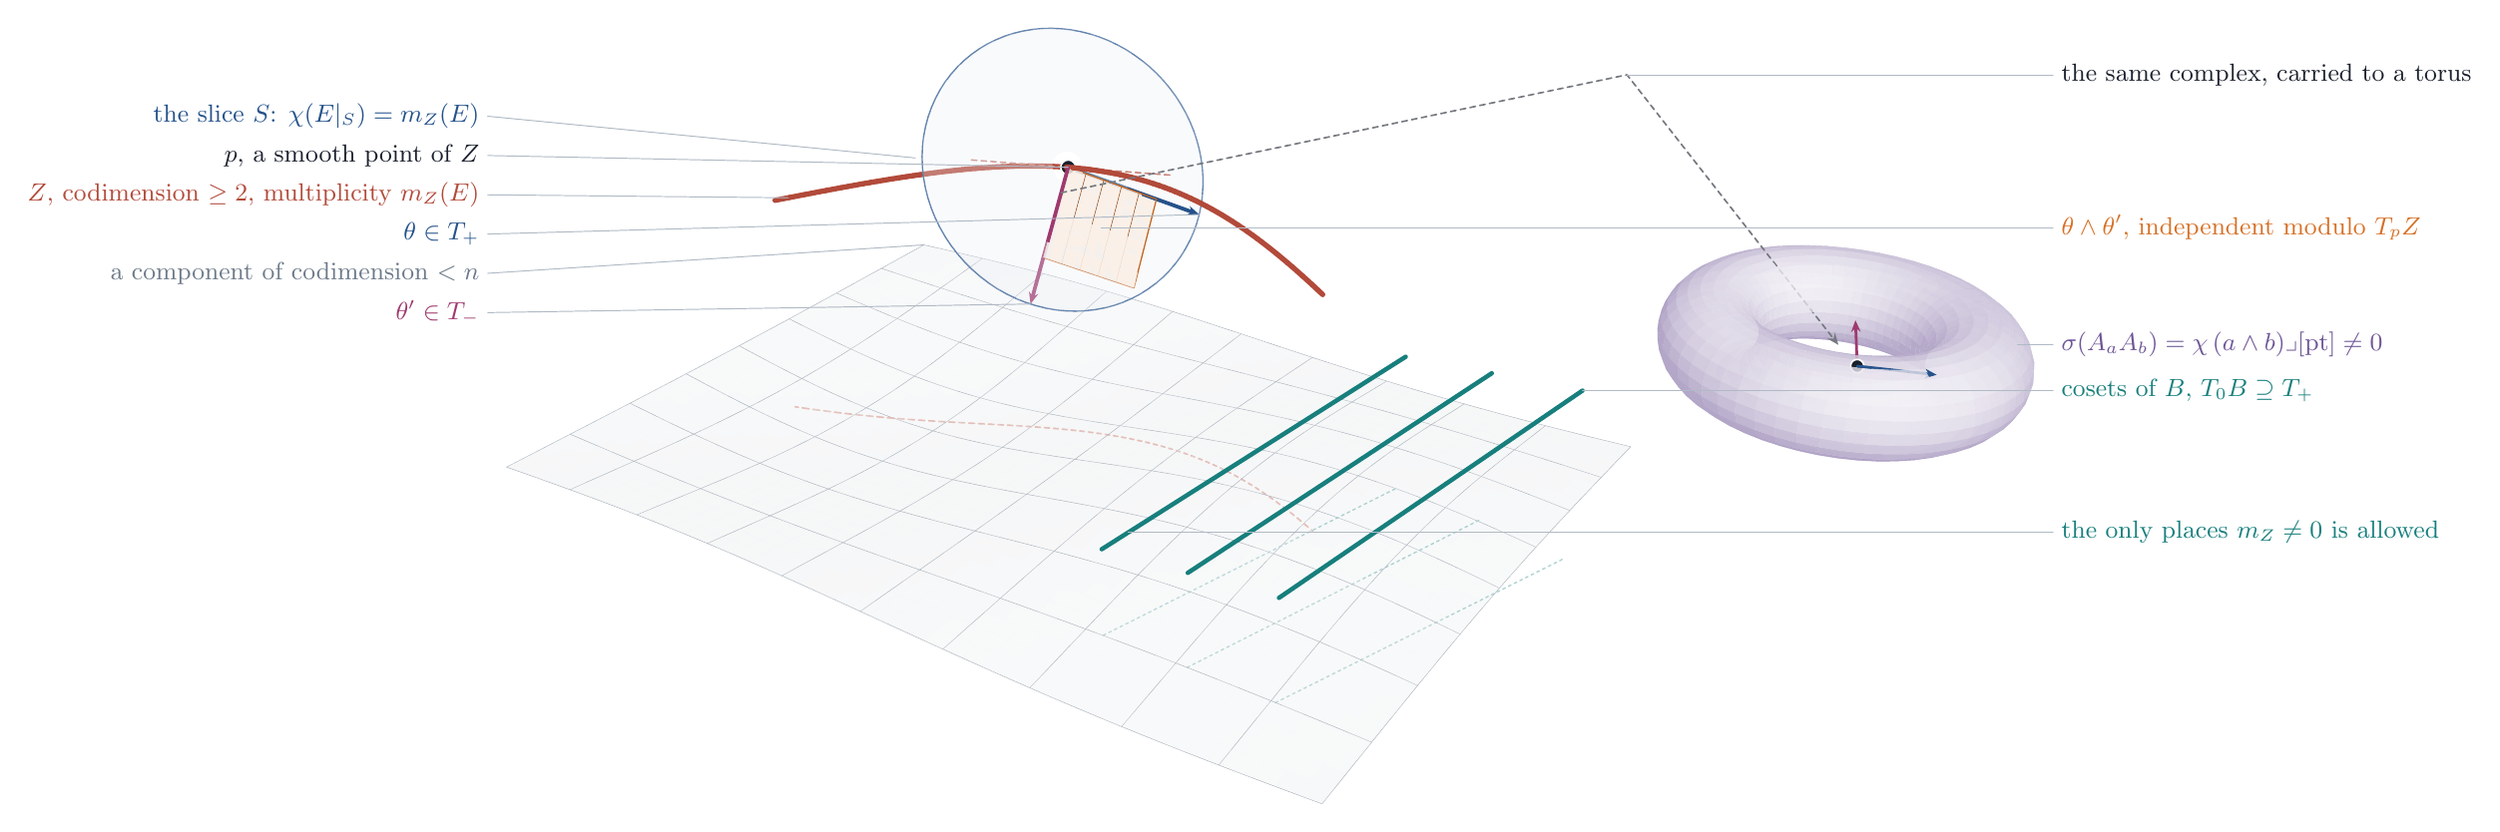
\begin{tikzpicture}[x=1cm,y=1cm,line join=round,line cap=round,
  font=\small,text=PInk]
  \draw[PSlate!55,line width=0.18pt] (-3.1177,1.1405) -- (-3.0234,1.1925);
  \path[draw=none,fill opacity=0.30,fill=PSlate!18!white] (-3.1522,1.1215) -- (-2.9887,1.0803) -- (-2.8606,1.1556) -- (-3.0234,1.1925) -- cycle;
  \draw[PSlate!55,line width=0.18pt] (-3.0234,1.1925) -- (-2.9014,1.1649) -- (-2.7786,1.1370) -- (-2.6550,1.1086) -- (-2.5306,1.0799);
  \path[draw=none,fill opacity=0.30,fill=PSlate!18!white] (-2.9887,1.0803) -- (-2.8238,1.0386) -- (-2.6963,1.1181) -- (-2.8606,1.1556) -- cycle;
  \path[draw=none,fill opacity=0.30,fill=PSlate!18!white] (-3.2826,1.0495) -- (-3.1184,1.0039) -- (-2.9887,1.0803) -- (-3.1522,1.1215) -- cycle;
  \draw[PSlate!55,line width=0.18pt] (-3.5036,0.9275) -- (-3.4058,0.9815) -- (-3.3089,1.0350) -- (-3.2129,1.0880) -- (-3.1177,1.1405);
  \path[draw=none,fill opacity=0.30,fill=PSlate!17!white] (-2.8238,1.0386) -- (-2.6574,0.9963) -- (-2.5306,1.0799) -- (-2.6963,1.1181) -- cycle;
  \path[draw=none,fill opacity=0.30,fill=PSlate!17!white] (-3.1184,1.0039) -- (-2.9528,0.9579) -- (-2.8238,1.0386) -- (-2.9887,1.0803) -- cycle;
  \path[draw=none,fill opacity=0.30,fill=PSlate!17!white] (-3.4146,0.9766) -- (-3.2497,0.9266) -- (-3.1184,1.0039) -- (-3.2826,1.0495) -- cycle;
  \path[draw=none,fill opacity=0.30,fill=PSlate!17!white] (-2.6574,0.9963) -- (-2.4896,0.9533) -- (-2.3634,1.0408) -- (-2.5306,1.0799) -- cycle;
  \draw[PSlate!55,line width=0.18pt] (-2.5306,1.0799) -- (-2.4053,1.0507) -- (-2.2792,1.0209) -- (-2.1523,0.9904) -- (-2.0245,0.9593);
  \path[draw=none,fill opacity=0.30,fill=PSlate!17!white] (-2.9528,0.9579) -- (-2.7858,0.9114) -- (-2.6574,0.9963) -- (-2.8238,1.0386) -- cycle;
  \path[draw=none,fill opacity=0.30,fill=PSlate!17!white] (-3.2497,0.9266) -- (-3.0834,0.8762) -- (-2.9528,0.9579) -- (-3.1184,1.0039) -- cycle;
  \draw[PSlate!55,line width=0.18pt] (-2.3714,0.9555) -- (-2.2792,1.0209);
  \path[draw=none,fill opacity=0.30,fill=PSlate!16!white] (-2.4896,0.9533) -- (-2.3203,0.9095) -- (-2.1947,1.0006) -- (-2.3634,1.0408) -- cycle;
  \path[draw=none,fill opacity=0.30,fill=PSlate!17!white] (-3.5483,0.9029) -- (-3.3827,0.8483) -- (-3.2497,0.9266) -- (-3.4146,0.9766) -- cycle;
  \path[draw=none,fill opacity=0.30,fill=PSlate!16!white] (-2.7858,0.9114) -- (-2.6174,0.8644) -- (-2.4896,0.9533) -- (-2.6574,0.9963) -- cycle;
  \path[draw=none,fill opacity=0.30,fill=PSlate!17!white] (-3.0834,0.8762) -- (-2.9158,0.8255) -- (-2.7858,0.9114) -- (-2.9528,0.9579) -- cycle;
  \path[draw=none,fill opacity=0.30,fill=PSlate!16!white] (-2.3203,0.9095) -- (-2.1495,0.8649) -- (-2.0245,0.9593) -- (-2.1947,1.0006) -- cycle;
  \path[draw=none,fill opacity=0.30,fill=PSlate!17!white] (-3.3827,0.8483) -- (-3.2157,0.7935) -- (-3.0834,0.8762) -- (-3.2497,0.9266) -- cycle;
  \path[draw=none,fill opacity=0.30,fill=PSlate!16!white] (-2.6174,0.8644) -- (-2.4475,0.8169) -- (-2.3203,0.9095) -- (-2.4896,0.9533) -- cycle;
  \path[draw=none,fill opacity=0.30,fill=PSlate!17!white] (-3.6837,0.8282) -- (-3.5173,0.7692) -- (-3.3827,0.8483) -- (-3.5483,0.9029) -- cycle;
  \path[draw=none,fill opacity=0.30,fill=PSlate!16!white] (-2.9158,0.8255) -- (-2.7466,0.7744) -- (-2.6174,0.8644) -- (-2.7858,0.9114) -- cycle;
  \path[draw=none,fill opacity=0.30,fill=PSlate!16!white] (-2.1495,0.8649) -- (-1.9772,0.8193) -- (-1.8527,0.9167) -- (-2.0245,0.9593) -- cycle;
  \draw[PSlate!55,line width=0.18pt] (-3.5652,0.8936) -- (-3.4410,0.8523) -- (-3.3160,0.8108) -- (-3.1903,0.7693) -- (-3.0638,0.7276);
  \draw[PSlate!55,line width=0.18pt] (-3.9039,0.7069) -- (-3.8024,0.7628) -- (-3.7019,0.8182) -- (-3.6023,0.8731) -- (-3.5036,0.9275);
  \path[draw=none,fill opacity=0.30,fill=PSlate!16!white] (-3.2157,0.7935) -- (-3.0473,0.7385) -- (-2.9158,0.8255) -- (-3.0834,0.8762) -- cycle;
  \draw[PSlate!55,line width=0.18pt] (-2.0245,0.9593) -- (-1.8958,0.9275) -- (-1.7663,0.8949) -- (-1.6359,0.8615) -- (-1.5046,0.8273);
  \draw[PSlate!55,line width=0.18pt] (-2.7484,0.6870) -- (-2.6529,0.7550) -- (-2.5583,0.8225) -- (-2.4644,0.8893) -- (-2.3714,0.9555);
  \path[draw=none,fill opacity=0.30,fill=PSlate!16!white] (-2.4475,0.8169) -- (-2.2761,0.7689) -- (-2.1495,0.8649) -- (-2.3203,0.9095) -- cycle;
  \path[draw=none,fill opacity=0.30,fill=PSlate!16!white] (-3.5173,0.7692) -- (-3.3496,0.7100) -- (-3.2157,0.7935) -- (-3.3827,0.8483) -- cycle;
  \path[draw=none,fill opacity=0.30,fill=PSlate!16!white] (-2.7466,0.7744) -- (-2.5761,0.7231) -- (-2.4475,0.8169) -- (-2.6174,0.8644) -- cycle;
  \path[draw=none,fill opacity=0.30,fill=PSlate!16!white] (-1.9772,0.8193) -- (-1.8034,0.7727) -- (-1.6794,0.8728) -- (-1.8527,0.9167) -- cycle;
  \path[draw=none,fill opacity=0.30,fill=PSlate!17!white] (-3.8208,0.7527) -- (-3.6536,0.6893) -- (-3.5173,0.7692) -- (-3.6837,0.8282) -- cycle;
  \path[draw=none,fill opacity=0.30,fill=PSlate!16!white] (-3.0473,0.7385) -- (-2.8775,0.6834) -- (-2.7466,0.7744) -- (-2.9158,0.8255) -- cycle;
  \path[draw=none,fill opacity=0.30,fill=PSlate!16!white] (-2.2761,0.7689) -- (-2.1032,0.7202) -- (-1.9772,0.8193) -- (-2.1495,0.8649) -- cycle;
  \path[draw=none,fill opacity=0.30,fill=PSlate!16!white] (-3.3496,0.7100) -- (-3.1805,0.6508) -- (-3.0473,0.7385) -- (-3.2157,0.7935) -- cycle;
  \path[draw=none,fill opacity=0.30,fill=PSlate!16!white] (-2.5761,0.7231) -- (-2.4041,0.6716) -- (-2.2761,0.7689) -- (-2.4475,0.8169) -- cycle;
  \path[draw=none,fill opacity=0.30,fill=PSlate!15!white] (-1.8034,0.7727) -- (-1.6280,0.7251) -- (-1.5046,0.8273) -- (-1.6794,0.8728) -- cycle;
  \path[draw=none,fill opacity=0.30,fill=PSlate!16!white] (-3.6536,0.6893) -- (-3.4851,0.6258) -- (-3.3496,0.7100) -- (-3.5173,0.7692) -- cycle;
  \path[draw=none,fill opacity=0.30,fill=PSlate!16!white] (-2.8775,0.6834) -- (-2.7063,0.6284) -- (-2.5761,0.7231) -- (-2.7466,0.7744) -- cycle;
  \draw[PSlate!55,line width=0.18pt] (-1.5949,0.7525) -- (-1.5046,0.8273);
  \path[draw=none,fill opacity=0.30,fill=PSlate!15!white] (-2.1032,0.7202) -- (-1.9288,0.6710) -- (-1.8034,0.7727) -- (-1.9772,0.8193) -- cycle;
  \path[draw=none,fill opacity=0.30,fill=PSlate!16!white] (-3.1805,0.6508) -- (-3.0100,0.5917) -- (-2.8775,0.6834) -- (-3.0473,0.7385) -- cycle;
  \path[draw=none,fill opacity=0.30,fill=PSlate!16!white] (-3.9597,0.6763) -- (-3.7917,0.6087) -- (-3.6536,0.6893) -- (-3.8208,0.7527) -- cycle;
  \path[draw=none,fill opacity=0.30,fill=PSlate!15!white] (-2.4041,0.6716) -- (-2.2306,0.6199) -- (-2.1032,0.7202) -- (-2.2761,0.7689) -- cycle;
  \draw[PSlate!55,line width=0.18pt] (-3.0638,0.7276) -- (-2.9366,0.6859) -- (-2.8085,0.6442) -- (-2.6797,0.6026) -- (-2.5500,0.5610);
  \path[draw=none,fill opacity=0.30,fill=PSlate!15!white] (-1.6280,0.7251) -- (-1.4510,0.6763) -- (-1.3282,0.7802) -- (-1.5046,0.8273) -- cycle;
  \path[draw=none,fill opacity=0.30,fill=PSlate!16!white] (-3.4851,0.6258) -- (-3.3153,0.5624) -- (-3.1805,0.6508) -- (-3.3496,0.7100) -- cycle;
  \path[draw=none,fill opacity=0.30,fill=PSlate!15!white] (-2.7063,0.6284) -- (-2.5337,0.5733) -- (-2.4041,0.6716) -- (-2.5761,0.7231) -- cycle;
  \draw[PSlate!55,line width=0.18pt] (-1.5046,0.8273) -- (-1.3724,0.7921) -- (-1.2394,0.7561) -- (-1.1054,0.7191) -- (-0.9706,0.6812);
  \path[draw=none,fill opacity=0.30,fill=PSlate!15!white] (-1.9288,0.6710) -- (-1.7528,0.6211) -- (-1.6280,0.7251) -- (-1.8034,0.7727) -- cycle;
  \path[draw=none,fill opacity=0.30,fill=PSlate!15!white] (-3.0100,0.5917) -- (-2.8381,0.5328) -- (-2.7063,0.6284) -- (-2.8775,0.6834) -- cycle;
  \path[draw=none,fill opacity=0.30,fill=PSlate!16!white] (-3.7917,0.6087) -- (-3.6225,0.5410) -- (-3.4851,0.6258) -- (-3.6536,0.6893) -- cycle;
  \path[draw=none,fill opacity=0.30,fill=PSlate!15!white] (-2.2306,0.6199) -- (-2.0557,0.5679) -- (-1.9288,0.6710) -- (-2.1032,0.7202) -- cycle;
  \path[draw=none,fill opacity=0.30,fill=PSlate!16!white] (-3.3153,0.5624) -- (-3.1441,0.4994) -- (-3.0100,0.5917) -- (-3.1805,0.6508) -- cycle;
  \path[draw=none,fill opacity=0.30,fill=PSlate!15!white] (-1.4510,0.6763) -- (-1.2725,0.6264) -- (-1.1502,0.7315) -- (-1.3282,0.7802) -- cycle;
  \path[draw=none,fill opacity=0.30,fill=PSlate!16!white] (-4.1004,0.5990) -- (-3.9316,0.5273) -- (-3.7917,0.6087) -- (-3.9597,0.6763) -- cycle;
  \path[draw=none,fill opacity=0.30,fill=PSlate!15!white] (-2.5337,0.5733) -- (-2.3596,0.5185) -- (-2.2306,0.6199) -- (-2.4041,0.6716) -- cycle;
  \path[draw=none,fill opacity=0.30,fill=PSlate!15!white] (-1.7528,0.6211) -- (-1.5754,0.5706) -- (-1.4510,0.6763) -- (-1.6280,0.7251) -- cycle;
  \draw[PSlate!55,line width=0.18pt] (-3.1391,0.4113) -- (-3.0401,0.4806) -- (-2.9420,0.5497) -- (-2.8447,0.6185) -- (-2.7484,0.6870);
  \draw[PSlate!55,line width=0.18pt] (-4.3196,0.4789) -- (-4.2142,0.5366) -- (-4.1098,0.5938) -- (-4.0064,0.6506) -- (-3.9039,0.7069);
  \path[draw=none,fill opacity=0.30,fill=PSlate!16!white] (-3.6225,0.5410) -- (-3.4519,0.4736) -- (-3.3153,0.5624) -- (-3.4851,0.6258) -- cycle;
  \path[draw=none,fill opacity=0.30,fill=PSlate!15!white] (-2.8381,0.5328) -- (-2.6649,0.4743) -- (-2.5337,0.5733) -- (-2.7063,0.6284) -- cycle;
  \path[draw=none,fill opacity=0.30,fill=PSlate!15!white] (-2.0557,0.5679) -- (-1.8792,0.5158) -- (-1.7528,0.6211) -- (-1.9288,0.6710) -- cycle;
  \draw[PSlate!55,line width=0.18pt] (-1.9642,0.4450) -- (-1.8707,0.5229) -- (-1.7780,0.6002) -- (-1.6861,0.6768) -- (-1.5949,0.7525);
  \path[draw=none,fill opacity=0.30,fill=PSlate!15!white] (-3.1441,0.4994) -- (-2.9716,0.4368) -- (-2.8381,0.5328) -- (-3.0100,0.5917) -- cycle;
  \path[draw=none,fill opacity=0.30,fill=PSlate!16!white] (-3.9316,0.5273) -- (-3.7616,0.4557) -- (-3.6225,0.5410) -- (-3.7917,0.6087) -- cycle;
  \path[draw=none,fill opacity=0.30,fill=PSlate!15!white] (-1.2725,0.6264) -- (-1.0924,0.5753) -- (-0.9706,0.6812) -- (-1.1502,0.7315) -- cycle;
  \path[draw=none,fill opacity=0.30,fill=PSlate!15!white] (-2.3596,0.5185) -- (-2.1841,0.4638) -- (-2.0557,0.5679) -- (-2.2306,0.6199) -- cycle;
  \path[draw=none,fill opacity=0.30,fill=PSlate!15!white] (-1.5754,0.5706) -- (-1.3963,0.5195) -- (-1.2725,0.6264) -- (-1.4510,0.6763) -- cycle;
  \path[draw=none,fill opacity=0.30,fill=PSlate!15!white] (-3.4519,0.4736) -- (-3.2800,0.4066) -- (-3.1441,0.4994) -- (-3.3153,0.5624) -- cycle;
  \path[draw=none,fill opacity=0.30,fill=PSlate!15!white] (-2.6649,0.4743) -- (-2.4902,0.4164) -- (-2.3596,0.5185) -- (-2.5337,0.5733) -- cycle;
  \path[draw=none,fill opacity=0.30,fill=PSlate!16!white] (-4.2429,0.5209) -- (-4.0734,0.4454) -- (-3.9316,0.5273) -- (-4.1004,0.5990) -- cycle;
  \path[draw=none,fill opacity=0.30,fill=PSlate!15!white] (-1.8792,0.5158) -- (-1.7012,0.4635) -- (-1.5754,0.5706) -- (-1.7528,0.6211) -- cycle;
  \path[draw=none,fill opacity=0.30,fill=PSlate!15!white] (-2.9716,0.4368) -- (-2.7977,0.3749) -- (-2.6649,0.4743) -- (-2.8381,0.5328) -- cycle;
  \path[draw=none,fill opacity=0.30,fill=PSlate!16!white] (-3.7616,0.4557) -- (-3.5903,0.3843) -- (-3.4519,0.4736) -- (-3.6225,0.5410) -- cycle;
  \draw[PSlate!55,line width=0.18pt] (-2.5500,0.5610) -- (-2.4195,0.5195) -- (-2.2882,0.4782) -- (-2.1561,0.4371) -- (-2.0231,0.3961);
  \path[draw=none,fill opacity=0.30,fill=PSlate!15!white] (-1.0924,0.5753) -- (-0.9107,0.5230) -- (-0.7894,0.6292) -- (-0.9706,0.6812) -- cycle;
  \path[draw=none,fill opacity=0.30,fill=PSlate!15!white] (-2.1841,0.4638) -- (-2.0070,0.4094) -- (-1.8792,0.5158) -- (-2.0557,0.5679) -- cycle;
  \draw[PSlate!55,line width=0.18pt] (-4.1358,0.5796) -- (-4.0092,0.5251) -- (-3.8819,0.4706) -- (-3.7539,0.4162) -- (-3.6252,0.3620);
  \draw[PSlate!55,line width=0.18pt] (-0.9706,0.6812) -- (-0.8348,0.6423) -- (-0.6982,0.6025) -- (-0.5607,0.5618) -- (-0.4222,0.5201);
  \path[draw=none,fill opacity=0.30,fill=PSlate!15!white] (-3.2800,0.4066) -- (-3.1068,0.3404) -- (-2.9716,0.4368) -- (-3.1441,0.4994) -- cycle;
  \path[draw=none,fill opacity=0.30,fill=PSlate!15!white] (-1.3963,0.5195) -- (-1.2157,0.4676) -- (-1.0924,0.5753) -- (-1.2725,0.6264) -- cycle;
  \path[draw=none,fill opacity=0.30,fill=PSlate!16!white] (-4.0734,0.4454) -- (-3.9026,0.3699) -- (-3.7616,0.4557) -- (-3.9316,0.5273) -- cycle;
  \path[draw=none,fill opacity=0.30,fill=PSlate!15!white] (-2.4902,0.4164) -- (-2.3141,0.3590) -- (-2.1841,0.4638) -- (-2.3596,0.5185) -- cycle;
  \path[draw=none,fill opacity=0.30,fill=PSlate!15!white] (-1.7012,0.4635) -- (-1.5216,0.4111) -- (-1.3963,0.5195) -- (-1.5754,0.5706) -- cycle;
  \draw[PSlate!55,line width=0.18pt] (-0.7868,0.5249) -- (-0.6982,0.6025);
  \path[draw=none,fill opacity=0.30,fill=PSlate!15!white] (-3.5903,0.3843) -- (-3.4177,0.3137) -- (-3.2800,0.4066) -- (-3.4519,0.4736) -- cycle;
  \path[draw=none,fill opacity=0.30,fill=PSlate!15!white] (-2.7977,0.3749) -- (-2.6224,0.3138) -- (-2.4902,0.4164) -- (-2.6649,0.4743) -- cycle;
  \path[draw=none,fill opacity=0.30,fill=PSlate!15!white] (-0.9107,0.5230) -- (-0.7273,0.4696) -- (-0.6066,0.5755) -- (-0.7894,0.6292) -- cycle;
  \path[draw=none,fill opacity=0.30,fill=PSlate!16!white] (-4.3873,0.4420) -- (-4.2170,0.3629) -- (-4.0734,0.4454) -- (-4.2429,0.5209) -- cycle;
  \path[draw=none,fill opacity=0.30,fill=PSlate!15!white] (-2.0070,0.4094) -- (-1.8285,0.3554) -- (-1.7012,0.4635) -- (-1.8792,0.5158) -- cycle;
  \path[draw=none,fill opacity=0.30,fill=PSlate!15!white] (-3.1068,0.3404) -- (-2.9322,0.2752) -- (-2.7977,0.3749) -- (-2.9716,0.4368) -- cycle;
  \path[draw=none,fill opacity=0.30,fill=PSlate!15!white] (-3.9026,0.3699) -- (-3.7305,0.2949) -- (-3.5903,0.3843) -- (-3.7616,0.4557) -- cycle;
  \path[draw=none,fill opacity=0.30,fill=PSlate!15!white] (-1.2157,0.4676) -- (-1.0334,0.4151) -- (-0.9107,0.5230) -- (-1.0924,0.5753) -- cycle;
  \path[draw=none,fill opacity=0.30,fill=PSlate!15!white] (-2.3141,0.3590) -- (-2.1364,0.3024) -- (-2.0070,0.4094) -- (-2.1841,0.4638) -- cycle;
  \path[draw=none,fill opacity=0.30,fill=PSlate!15!white] (-1.5216,0.4111) -- (-1.3404,0.3585) -- (-1.2157,0.4676) -- (-1.3963,0.5195) -- cycle;
  \path[draw=none,fill opacity=0.30,fill=PSlate!15!white] (-3.4177,0.3137) -- (-3.2437,0.2440) -- (-3.1068,0.3404) -- (-3.2800,0.4066) -- cycle;
  \path[draw=none,fill opacity=0.30,fill=PSlate!15!white] (-2.6224,0.3138) -- (-2.4457,0.2538) -- (-2.3141,0.3590) -- (-2.4902,0.4164) -- cycle;
  \path[draw=none,fill opacity=0.30,fill=PSlate!16!white] (-4.2170,0.3629) -- (-4.0454,0.2838) -- (-3.9026,0.3699) -- (-4.0734,0.4454) -- cycle;
  \path[draw=none,fill opacity=0.30,fill=PSlate!15!white] (-0.7273,0.4696) -- (-0.5424,0.4150) -- (-0.4222,0.5201) -- (-0.6066,0.5755) -- cycle;
  \path[draw=none,fill opacity=0.30,fill=PSlate!15!white] (-1.8285,0.3554) -- (-1.6484,0.3016) -- (-1.5216,0.4111) -- (-1.7012,0.4635) -- cycle;
  \path[draw=none,fill opacity=0.30,fill=PSlate!15!white] (-2.9322,0.2752) -- (-2.7563,0.2112) -- (-2.6224,0.3138) -- (-2.7977,0.3749) -- cycle;
  \path[draw=none,fill opacity=0.30,fill=PSlate!15!white] (-3.7305,0.2949) -- (-3.5571,0.2207) -- (-3.4177,0.3137) -- (-3.5903,0.3843) -- cycle;
  \path[draw=none,fill opacity=0.30,fill=PSlate!15!white] (-1.0334,0.4151) -- (-0.8495,0.3619) -- (-0.7273,0.4696) -- (-0.9107,0.5230) -- cycle;
  \path[draw=none,fill opacity=0.30,fill=PSlate!15!white] (-2.1364,0.3024) -- (-1.9573,0.2465) -- (-1.8285,0.3554) -- (-2.0070,0.4094) -- cycle;
  \path[draw=none,fill opacity=0.30,fill=PSlate!16!white] (-4.5336,0.3623) -- (-4.3625,0.2798) -- (-4.2170,0.3629) -- (-4.3873,0.4420) -- cycle;
  \draw[PSlate!55,line width=0.18pt] (-3.5449,0.1337) -- (-3.4420,0.2030) -- (-3.3401,0.2724) -- (-3.2391,0.3418) -- (-3.1391,0.4113);
  \path[draw=none,fill opacity=0.30,fill=PSlate!15!white] (-3.2437,0.2440) -- (-3.0685,0.1756) -- (-2.9322,0.2752) -- (-3.1068,0.3404) -- cycle;
  \path[draw=none,fill opacity=0.30,fill=PSlate!15!white] (-1.3404,0.3585) -- (-1.1576,0.3057) -- (-1.0334,0.4151) -- (-1.2157,0.4676) -- cycle;
  \draw[PSlate!55,line width=0.18pt] (-2.3469,0.1305) -- (-2.2499,0.2093) -- (-2.1538,0.2881) -- (-2.0586,0.3667) -- (-1.9642,0.4450);
  \path[draw=none,fill opacity=0.30,fill=PSlate!15!white] (-2.4457,0.2538) -- (-2.2675,0.1949) -- (-2.1364,0.3024) -- (-2.3141,0.3590) -- cycle;
  \path[draw=none,fill opacity=0.30,fill=PSlate!15!white] (-4.0454,0.2838) -- (-3.8726,0.2054) -- (-3.7305,0.2949) -- (-3.9026,0.3699) -- cycle;
  \draw[PSlate!55,line width=0.18pt] (-4.7517,0.2438) -- (-4.6421,0.3033) -- (-4.5336,0.3623) -- (-4.4261,0.4208) -- (-4.3196,0.4789);
  \draw[PSlate!55,line width=0.18pt] (-3.6252,0.3620) -- (-3.4957,0.3082) -- (-3.3655,0.2550) -- (-3.2345,0.2025) -- (-3.1028,0.1507);
  \draw[PSlate!55,line width=0.18pt] (-2.0231,0.3961) -- (-1.8893,0.3553) -- (-1.7546,0.3148) -- (-1.6190,0.2745) -- (-1.4826,0.2344);
  \path[draw=none,fill opacity=0.30,fill=PSlate!15!white] (-0.5424,0.4150) -- (-0.3558,0.3592) -- (-0.2362,0.4632) -- (-0.4222,0.5201) -- cycle;
  \path[draw=none,fill opacity=0.30,fill=PSlate!15!white] (-1.6484,0.3016) -- (-1.4667,0.2482) -- (-1.3404,0.3585) -- (-1.5216,0.4111) -- cycle;
  \path[draw=none,fill opacity=0.30,fill=PSlate!15!white] (-3.5571,0.2207) -- (-3.3825,0.1477) -- (-3.2437,0.2440) -- (-3.4177,0.3137) -- cycle;
  \path[draw=none,fill opacity=0.30,fill=PSlate!15!white] (-2.7563,0.2112) -- (-2.5789,0.1486) -- (-2.4457,0.2538) -- (-2.6224,0.3138) -- cycle;
  \draw[PSlate!55,line width=0.18pt] (-0.4222,0.5201) -- (-0.2829,0.4775) -- (-0.1426,0.4341) -- (-0.0014,0.3898) -- (0.1407,0.3447);
  \draw[PSlate!55,line width=0.18pt] (-1.1491,0.2057) -- (-1.0573,0.2866) -- (-0.9664,0.3668) -- (-0.8762,0.4463) -- (-0.7868,0.5249);
  \path[draw=none,fill opacity=0.30,fill=PSlate!15!white] (-0.8495,0.3619) -- (-0.6640,0.3080) -- (-0.5424,0.4150) -- (-0.7273,0.4696) -- cycle;
  \path[draw=none,fill opacity=0.30,fill=PSlate!15!white] (-4.3625,0.2798) -- (-4.1902,0.1975) -- (-4.0454,0.2838) -- (-4.2170,0.3629) -- cycle;
  \path[draw=none,fill opacity=0.30,fill=PSlate!15!white] (-1.9573,0.2465) -- (-1.7767,0.1915) -- (-1.6484,0.3016) -- (-1.8285,0.3554) -- cycle;
  \path[draw=none,fill opacity=0.30,fill=PSlate!15!white] (-3.0685,0.1756) -- (-2.8919,0.1087) -- (-2.7563,0.2112) -- (-2.9322,0.2752) -- cycle;
  \path[draw=none,fill opacity=0.30,fill=PSlate!15!white] (-3.8726,0.2054) -- (-3.6985,0.1279) -- (-3.5571,0.2207) -- (-3.7305,0.2949) -- cycle;
  \path[draw=none,fill opacity=0.30,fill=PSlate!15!white] (-1.1576,0.3057) -- (-0.9732,0.2528) -- (-0.8495,0.3619) -- (-1.0334,0.4151) -- cycle;
  \path[draw=none,fill opacity=0.30,fill=PSlate!15!white] (-2.2675,0.1949) -- (-2.0878,0.1373) -- (-1.9573,0.2465) -- (-2.1364,0.3024) -- cycle;
  \path[draw=none,fill opacity=0.30,fill=PSlate!15!white] (-0.3558,0.3592) -- (-0.1675,0.3023) -- (-0.0486,0.4046) -- (-0.2362,0.4632) -- cycle;
  \path[draw=none,fill opacity=0.30,fill=PSlate!16!white] (-4.6819,0.2817) -- (-4.5100,0.1962) -- (-4.3625,0.2798) -- (-4.5336,0.3623) -- cycle;
  \path[draw=none,fill opacity=0.30,fill=PSlate!15!white] (-1.4667,0.2482) -- (-1.2834,0.1952) -- (-1.1576,0.3057) -- (-1.3404,0.3585) -- cycle;
  \path[draw=none,fill opacity=0.30,fill=PSlate!15!white] (-3.3825,0.1477) -- (-3.2066,0.0763) -- (-3.0685,0.1756) -- (-3.2437,0.2440) -- cycle;
  \path[draw=none,fill opacity=0.30,fill=PSlate!15!white] (-2.5789,0.1486) -- (-2.4002,0.0875) -- (-2.2675,0.1949) -- (-2.4457,0.2538) -- cycle;
  \path[draw=none,fill opacity=0.30,fill=PSlate!15!white] (-4.1902,0.1975) -- (-4.0166,0.1158) -- (-3.8726,0.2054) -- (-4.0454,0.2838) -- cycle;
  \path[draw=none,fill opacity=0.30,fill=PSlate!15!white] (-0.6640,0.3080) -- (-0.4768,0.2535) -- (-0.3558,0.3592) -- (-0.5424,0.4150) -- cycle;
  \path[draw=none,fill opacity=0.30,fill=PSlate!15!white] (-1.7767,0.1915) -- (-1.5945,0.1373) -- (-1.4667,0.2482) -- (-1.6484,0.3016) -- cycle;
  \path[draw=none,fill opacity=0.30,fill=PSlate!15!white] (-2.8919,0.1087) -- (-2.7140,0.0435) -- (-2.5789,0.1486) -- (-2.7563,0.2112) -- cycle;
  \path[draw=none,fill opacity=0.30,fill=PSlate!15!white] (-3.6985,0.1279) -- (-3.5231,0.0518) -- (-3.3825,0.1477) -- (-3.5571,0.2207) -- cycle;
  \path[draw=none,fill opacity=0.30,fill=PSlate!15!white] (-0.9732,0.2528) -- (-0.7871,0.1997) -- (-0.6640,0.3080) -- (-0.8495,0.3619) -- cycle;
  \path[draw=none,fill opacity=0.30,fill=PSlate!15!white] (-2.0878,0.1373) -- (-1.9066,0.0810) -- (-1.7767,0.1915) -- (-1.9573,0.2465) -- cycle;
  \path[draw=none,fill opacity=0.30,fill=PSlate!15!white] (-4.5100,0.1962) -- (-4.3369,0.1110) -- (-4.1902,0.1975) -- (-4.3625,0.2798) -- cycle;
  \path[draw=none,fill opacity=0.30,fill=PSlate!15!white] (-0.1675,0.3023) -- (0.0224,0.2443) -- (0.1407,0.3447) -- (-0.0486,0.4046) -- cycle;
  \path[draw=none,fill opacity=0.30,fill=PSlate!15!white] (-3.2066,0.0763) -- (-3.0293,0.0066) -- (-2.8919,0.1087) -- (-3.0685,0.1756) -- cycle;
  \path[draw=none,fill opacity=0.30,fill=PSlate!15!white] (-1.2834,0.1952) -- (-1.0984,0.1425) -- (-0.9732,0.2528) -- (-1.1576,0.3057) -- cycle;
  \path[draw=none,fill opacity=0.30,fill=PSlate!15!white] (-4.0166,0.1158) -- (-3.8418,0.0353) -- (-3.6985,0.1279) -- (-3.8726,0.2054) -- cycle;
  \path[draw=none,fill opacity=0.30,fill=PSlate!15!white] (-2.4002,0.0875) -- (-2.2199,0.0281) -- (-2.0878,0.1373) -- (-2.2675,0.1949) -- cycle;
  \draw[PSlate!55,line width=0.18pt] (0.0541,0.2713) -- (0.1407,0.3447);
  \path[draw=none,fill opacity=0.30,fill=PSlate!15!white] (-0.4768,0.2535) -- (-0.2880,0.1983) -- (-0.1675,0.3023) -- (-0.3558,0.3592) -- cycle;
  \path[draw=none,fill opacity=0.30,fill=PSlate!15!white] (-1.5945,0.1373) -- (-1.4106,0.0840) -- (-1.2834,0.1952) -- (-1.4667,0.2482) -- cycle;
  \path[draw=none,fill opacity=0.30,fill=PSlate!16!white] (-4.8321,0.2003) -- (-4.6596,0.1122) -- (-4.5100,0.1962) -- (-4.6819,0.2817) -- cycle;
  \path[draw=none,fill opacity=0.30,fill=PSlate!15!white] (-3.5231,0.0518) -- (-3.3465,-0.0226) -- (-3.2066,0.0763) -- (-3.3825,0.1477) -- cycle;
  \path[draw=none,fill opacity=0.30,fill=PSlate!15!white] (-2.7140,0.0435) -- (-2.5346,-0.0197) -- (-2.4002,0.0875) -- (-2.5789,0.1486) -- cycle;
  \draw[PSlate!55,line width=0.18pt] (-3.1028,0.1507) -- (-2.9704,0.0999) -- (-2.8372,0.0500) -- (-2.7032,0.0012) -- (-2.5685,-0.0464);
  \path[draw=none,fill opacity=0.30,fill=PSlate!15!white] (-4.3369,0.1110) -- (-4.1626,0.0265) -- (-4.0166,0.1158) -- (-4.1902,0.1975) -- cycle;
  \path[draw=none,fill opacity=0.30,fill=PSlate!15!white] (-0.7871,0.1997) -- (-0.5994,0.1463) -- (-0.4768,0.2535) -- (-0.6640,0.3080) -- cycle;
  \path[draw=none,fill opacity=0.30,fill=PSlate!15!white] (-1.9066,0.0810) -- (-1.7239,0.0260) -- (-1.5945,0.1373) -- (-1.7767,0.1915) -- cycle;
  \path[draw=none,fill opacity=0.30,fill=PSlate!15!white] (0.0224,0.2443) -- (0.2140,0.1854) -- (0.3316,0.2833) -- (0.1407,0.3447) -- cycle;
  \draw[PSlate!55,line width=0.18pt] (-1.4826,0.2344) -- (-1.3452,0.1946) -- (-1.2069,0.1550) -- (-1.0677,0.1156) -- (-0.9275,0.0764);
  \path[draw=none,fill opacity=0.30,fill=PSlate!15!white] (-3.0293,0.0066) -- (-2.8508,-0.0610) -- (-2.7140,0.0435) -- (-2.8919,0.1087) -- cycle;
  \path[draw=none,fill opacity=0.30,fill=PSlate!15!white] (-3.8418,0.0353) -- (-3.6657,-0.0436) -- (-3.5231,0.0518) -- (-3.6985,0.1279) -- cycle;
  \path[draw=none,fill opacity=0.30,fill=PSlate!15!white] (-1.0984,0.1425) -- (-0.9118,0.0901) -- (-0.7871,0.1997) -- (-0.9732,0.2528) -- cycle;
  \draw[PSlate!55,line width=0.18pt] (-4.7380,0.2513) -- (-4.6090,0.1864) -- (-4.4793,0.1216) -- (-4.3490,0.0570) -- (-4.2179,-0.0070);
  \path[draw=none,fill opacity=0.30,fill=PSlate!15!white] (-2.2199,0.0281) -- (-2.0382,-0.0296) -- (-1.9066,0.0810) -- (-2.0878,0.1373) -- cycle;
  \draw[PSlate!55,line width=0.18pt] (0.1407,0.3447) -- (0.2837,0.2988) -- (0.4277,0.2522) -- (0.5726,0.2050) -- (0.7184,0.1571);
  \path[draw=none,fill opacity=0.30,fill=PSlate!15!white] (-4.6596,0.1122) -- (-4.4857,0.0244) -- (-4.3369,0.1110) -- (-4.5100,0.1962) -- cycle;
  \path[draw=none,fill opacity=0.30,fill=PSlate!15!white] (-0.2880,0.1983) -- (-0.0974,0.1424) -- (0.0224,0.2443) -- (-0.1675,0.3023) -- cycle;
  \path[draw=none,fill opacity=0.30,fill=PSlate!15!white] (-1.4106,0.0840) -- (-1.2252,0.0315) -- (-1.0984,0.1425) -- (-1.2834,0.1952) -- cycle;
  \path[draw=none,fill opacity=0.30,fill=PSlate!15!white] (-3.3465,-0.0226) -- (-3.1687,-0.0948) -- (-3.0293,0.0066) -- (-3.2066,0.0763) -- cycle;
  \path[draw=none,fill opacity=0.30,fill=PSlate!15!white] (-2.5346,-0.0197) -- (-2.3538,-0.0808) -- (-2.2199,0.0281) -- (-2.4002,0.0875) -- cycle;
  \path[draw=none,fill opacity=0.30,fill=PSlate!15!white] (-4.1626,0.0265) -- (-3.9871,-0.0568) -- (-3.8418,0.0353) -- (-4.0166,0.1158) -- cycle;
  \path[draw=none,fill opacity=0.30,fill=PSlate!15!white] (-0.5994,0.1463) -- (-0.4099,0.0928) -- (-0.2880,0.1983) -- (-0.4768,0.2535) -- cycle;
  \draw[PSlate!55,line width=0.18pt] (-3.9672,-0.1412) -- (-3.8600,-0.0730) -- (-3.7539,-0.0044) -- (-3.6489,0.0645) -- (-3.5449,0.1337);
  \path[draw=none,fill opacity=0.30,fill=PSlate!15!white] (-1.7239,0.0260) -- (-1.5395,-0.0277) -- (-1.4106,0.0840) -- (-1.5945,0.1373) -- cycle;
  \draw[PSlate!55,line width=0.18pt] (-2.7442,-0.1827) -- (-2.6434,-0.1050) -- (-2.5436,-0.0268) -- (-2.4448,0.0517) -- (-2.3469,0.1305);
  \path[draw=none,fill opacity=0.30,fill=PSlate!16!white] (0.2140,0.1854) -- (0.4073,0.1255) -- (0.5242,0.2208) -- (0.3316,0.2833) -- cycle;
  \path[draw=none,fill opacity=0.30,fill=PSlate!15!white] (-2.8508,-0.0610) -- (-2.6708,-0.1262) -- (-2.5346,-0.0197) -- (-2.7140,0.0435) -- cycle;
  \path[draw=none,fill opacity=0.30,fill=PSlate!15!white] (-3.6657,-0.0436) -- (-3.4885,-0.1206) -- (-3.3465,-0.0226) -- (-3.5231,0.0518) -- cycle;
  \path[draw=none,fill opacity=0.30,fill=PSlate!15!white] (-4.9845,0.1181) -- (-4.8112,0.0277) -- (-4.6596,0.1122) -- (-4.8321,0.2003) -- cycle;
  \path[draw=none,fill opacity=0.30,fill=PSlate!15!white] (-0.9118,0.0901) -- (-0.7235,0.0380) -- (-0.5994,0.1463) -- (-0.7871,0.1997) -- cycle;
  \path[draw=none,fill opacity=0.30,fill=PSlate!15!white] (-2.0382,-0.0296) -- (-1.8549,-0.0854) -- (-1.7239,0.0260) -- (-1.9066,0.0810) -- cycle;
  \draw[PSlate!55,line width=0.18pt] (-5.2013,0.0016) -- (-5.0872,0.0628) -- (-4.9742,0.1236) -- (-4.8624,0.1839) -- (-4.7517,0.2438);
  \path[draw=none,fill opacity=0.30,fill=PSlate!15!white] (-4.4857,0.0244) -- (-4.3107,-0.0627) -- (-4.1626,0.0265) -- (-4.3369,0.1110) -- cycle;
  \draw[PSlate!55,line width=0.18pt] (-1.5247,-0.1210) -- (-1.4295,-0.0391) -- (-1.3352,0.0428) -- (-1.2417,0.1244) -- (-1.1491,0.2057);
  \path[draw=none,fill opacity=0.30,fill=PSlate!16!white] (-0.0974,0.1424) -- (0.0949,0.0858) -- (0.2140,0.1854) -- (0.0224,0.2443) -- cycle;
  \path[draw=none,fill opacity=0.30,fill=PSlate!15!white] (-3.1687,-0.0948) -- (-2.9894,-0.1647) -- (-2.8508,-0.0610) -- (-3.0293,0.0066) -- cycle;
  \path[draw=none,fill opacity=0.30,fill=PSlate!15!white] (-1.2252,0.0315) -- (-1.0380,-0.0202) -- (-0.9118,0.0901) -- (-1.0984,0.1425) -- cycle;
  \path[draw=none,fill opacity=0.30,fill=PSlate!15!white] (-3.9871,-0.0568) -- (-3.8103,-0.1384) -- (-3.6657,-0.0436) -- (-3.8418,0.0353) -- cycle;
  \path[draw=none,fill opacity=0.30,fill=PSlate!15!white] (-2.3538,-0.0808) -- (-2.1715,-0.1397) -- (-2.0382,-0.0296) -- (-2.2199,0.0281) -- cycle;
  \path[draw=none,fill opacity=0.30,fill=PSlate!16!white] (-0.4099,0.0928) -- (-0.2187,0.0390) -- (-0.0974,0.1424) -- (-0.2880,0.1983) -- cycle;
  \path[draw=none,fill opacity=0.30,fill=PSlate!15!white] (-1.5395,-0.0277) -- (-1.3535,-0.0800) -- (-1.2252,0.0315) -- (-1.4106,0.0840) -- cycle;
  \path[draw=none,fill opacity=0.30,fill=PSlate!15!white] (-4.8112,0.0277) -- (-4.6367,-0.0623) -- (-4.4857,0.0244) -- (-4.6596,0.1122) -- cycle;
  \draw[PSlate!55,line width=0.18pt] (-0.3004,-0.0306) -- (-0.2106,0.0459) -- (-0.1215,0.1218) -- (-0.0333,0.1969) -- (0.0541,0.2713);
  \path[draw=none,fill opacity=0.30,fill=PSlate!16!white] (0.4073,0.1255) -- (0.6024,0.0647) -- (0.7184,0.1571) -- (0.5242,0.2208) -- cycle;
  \path[draw=none,fill opacity=0.30,fill=PSlate!15!white] (-3.4885,-0.1206) -- (-3.3099,-0.1953) -- (-3.1687,-0.0948) -- (-3.3465,-0.0226) -- cycle;
  \path[draw=none,fill opacity=0.30,fill=PSlate!15!white] (-2.6708,-0.1262) -- (-2.4894,-0.1890) -- (-2.3538,-0.0808) -- (-2.5346,-0.0197) -- cycle;
  \path[draw=none,fill opacity=0.30,fill=PSlate!15!white] (-4.3107,-0.0627) -- (-4.1345,-0.1484) -- (-3.9871,-0.0568) -- (-4.1626,0.0265) -- cycle;
  \path[draw=none,fill opacity=0.30,fill=PSlate!16!white] (-0.7235,0.0380) -- (-0.5334,-0.0138) -- (-0.4099,0.0928) -- (-0.5994,0.1463) -- cycle;
  \path[draw=none,fill opacity=0.30,fill=PSlate!15!white] (-1.8549,-0.0854) -- (-1.6700,-0.1394) -- (-1.5395,-0.0277) -- (-1.7239,0.0260) -- cycle;
  \path[draw=none,fill opacity=0.30,fill=PSlate!16!white] (0.0949,0.0858) -- (0.2890,0.0286) -- (0.4073,0.1255) -- (0.2140,0.1854) -- cycle;
  \path[draw=none,fill opacity=0.30,fill=PSlate!15!white] (-2.9894,-0.1647) -- (-2.8089,-0.2319) -- (-2.6708,-0.1262) -- (-2.8508,-0.0610) -- cycle;
  \path[draw=none,fill opacity=0.30,fill=PSlate!15!white] (-3.8103,-0.1384) -- (-3.6324,-0.2178) -- (-3.4885,-0.1206) -- (-3.6657,-0.0436) -- cycle;
  \path[draw=none,fill opacity=0.30,fill=PSlate!15!white] (-5.1389,0.0350) -- (-4.9649,-0.0572) -- (-4.8112,0.0277) -- (-4.9845,0.1181) -- cycle;
  \path[draw=none,fill opacity=0.30,fill=PSlate!16!white] (-1.0380,-0.0202) -- (-0.8491,-0.0711) -- (-0.7235,0.0380) -- (-0.9118,0.0901) -- cycle;
  \path[draw=none,fill opacity=0.30,fill=PSlate!15!white] (-2.1715,-0.1397) -- (-1.9877,-0.1964) -- (-1.8549,-0.0854) -- (-2.0382,-0.0296) -- cycle;
  \draw[PSlate!55,line width=0.18pt] (-2.5685,-0.0464) -- (-2.4329,-0.0927) -- (-2.2965,-0.1378) -- (-2.1593,-0.1816) -- (-2.0212,-0.2240);
  \path[draw=none,fill opacity=0.30,fill=PSlate!15!white] (-4.6367,-0.0623) -- (-4.4609,-0.1516) -- (-4.3107,-0.0627) -- (-4.4857,0.0244) -- cycle;
  \path[draw=none,fill opacity=0.30,fill=PSlate!16!white] (-0.2187,0.0390) -- (-0.0257,-0.0151) -- (0.0949,0.0858) -- (-0.0974,0.1424) -- cycle;
  \draw[PSlate!55,line width=0.18pt] (-4.2179,-0.0070) -- (-4.0862,-0.0703) -- (-3.9538,-0.1327) -- (-3.8207,-0.1940) -- (-3.6869,-0.2540);
  \path[draw=none,fill opacity=0.30,fill=PSlate!15!white] (-3.3099,-0.1953) -- (-3.1301,-0.2673) -- (-2.9894,-0.1647) -- (-3.1687,-0.0948) -- cycle;
  \path[draw=none,fill opacity=0.30,fill=PSlate!16!white] (-1.3535,-0.0800) -- (-1.1658,-0.1310) -- (-1.0380,-0.0202) -- (-1.2252,0.0315) -- cycle;
  \path[draw=none,fill opacity=0.30,fill=PSlate!16!white] (0.6024,0.0647) -- (0.7992,0.0031) -- (0.9143,0.0924) -- (0.7184,0.1571) -- cycle;
  \path[draw=none,fill opacity=0.30,fill=PSlate!15!white] (-2.4894,-0.1890) -- (-2.3066,-0.2492) -- (-2.1715,-0.1397) -- (-2.3538,-0.0808) -- cycle;
  \path[draw=none,fill opacity=0.30,fill=PSlate!15!white] (-4.1345,-0.1484) -- (-3.9570,-0.2323) -- (-3.8103,-0.1384) -- (-3.9871,-0.0568) -- cycle;
  \draw[PSlate!55,line width=0.18pt] (-0.9275,0.0764) -- (-0.7864,0.0374) -- (-0.6442,-0.0014) -- (-0.5011,-0.0401) -- (-0.3570,-0.0787);
  \draw[PSlate!55,line width=0.18pt] (0.7184,0.1571) -- (0.8652,0.1087) -- (1.0129,0.0598) -- (1.1617,0.0105) -- (1.3114,-0.0392);
  \path[draw=none,fill opacity=0.30,fill=PSlate!16!white] (-0.5334,-0.0138) -- (-0.3416,-0.0656) -- (-0.2187,0.0390) -- (-0.4099,0.0928) -- cycle;
  \path[draw=none,fill opacity=0.30,fill=PSlate!16!white] (-1.6700,-0.1394) -- (-1.4835,-0.1915) -- (-1.3535,-0.0800) -- (-1.5395,-0.0277) -- cycle;
  \path[draw=none,fill opacity=0.30,fill=PSlate!15!white] (-4.9649,-0.0572) -- (-4.7897,-0.1491) -- (-4.6367,-0.0623) -- (-4.8112,0.0277) -- cycle;
  \path[draw=none,fill opacity=0.30,fill=PSlate!15!white] (-3.6324,-0.2178) -- (-3.4532,-0.2947) -- (-3.3099,-0.1953) -- (-3.4885,-0.1206) -- cycle;
  \path[draw=none,fill opacity=0.30,fill=PSlate!15!white] (-2.8089,-0.2319) -- (-2.6269,-0.2963) -- (-2.4894,-0.1890) -- (-2.6708,-0.1262) -- cycle;
  \path[draw=none,fill opacity=0.30,fill=PSlate!16!white] (0.2890,0.0286) -- (0.4848,-0.0292) -- (0.6024,0.0647) -- (0.4073,0.1255) -- cycle;
  \path[draw=none,fill opacity=0.30,fill=PSlate!16!white] (-0.8491,-0.0711) -- (-0.6585,-0.1214) -- (-0.5334,-0.0138) -- (-0.7235,0.0380) -- cycle;
  \path[draw=none,fill opacity=0.30,fill=PSlate!15!white] (-1.9877,-0.1964) -- (-1.8023,-0.2507) -- (-1.6700,-0.1394) -- (-1.8549,-0.0854) -- cycle;
  \path[draw=none,fill opacity=0.30,fill=PSlate!15!white] (-4.4609,-0.1516) -- (-4.2840,-0.2394) -- (-4.1345,-0.1484) -- (-4.3107,-0.0627) -- cycle;
  \draw[PSlate!55,line width=0.18pt] (0.9290,-0.0044) -- (1.0129,0.0598);
  \path[draw=none,fill opacity=0.30,fill=PSlate!16!white] (-0.0257,-0.0151) -- (0.1691,-0.0695) -- (0.2890,0.0286) -- (0.0949,0.0858) -- cycle;
  \path[draw=none,fill opacity=0.30,fill=PSlate!15!white] (-3.1301,-0.2673) -- (-2.9489,-0.3364) -- (-2.8089,-0.2319) -- (-2.9894,-0.1647) -- cycle;
  \path[draw=none,fill opacity=0.30,fill=PSlate!17!white] (0.7992,0.0031) -- (0.9977,-0.0592) -- (1.1120,0.0270) -- (0.9143,0.0924) -- cycle;
  \path[draw=none,fill opacity=0.30,fill=PSlate!15!white] (-3.9570,-0.2323) -- (-3.7784,-0.3139) -- (-3.6324,-0.2178) -- (-3.8103,-0.1384) -- cycle;
  \path[draw=none,fill opacity=0.30,fill=PSlate!16!white] (-1.1658,-0.1310) -- (-0.9764,-0.1808) -- (-0.8491,-0.0711) -- (-1.0380,-0.0202) -- cycle;
  \path[draw=none,fill opacity=0.30,fill=PSlate!15!white] (-2.3066,-0.2492) -- (-2.1222,-0.3067) -- (-1.9877,-0.1964) -- (-2.1715,-0.1397) -- cycle;
  \path[draw=none,fill opacity=0.30,fill=PSlate!15!white] (-5.2955,-0.0489) -- (-5.1209,-0.1425) -- (-4.9649,-0.0572) -- (-5.1389,0.0350) -- cycle;
  \path[draw=none,fill opacity=0.30,fill=PSlate!15!white] (-4.7897,-0.1491) -- (-4.6133,-0.2401) -- (-4.4609,-0.1516) -- (-4.6367,-0.0623) -- cycle;
  \path[draw=none,fill opacity=0.30,fill=PSlate!16!white] (-0.3416,-0.0656) -- (-0.1479,-0.1172) -- (-0.0257,-0.0151) -- (-0.2187,0.0390) -- cycle;
  \path[draw=none,fill opacity=0.30,fill=PSlate!16!white] (-1.4835,-0.1915) -- (-1.2953,-0.2419) -- (-1.1658,-0.1310) -- (-1.3535,-0.0800) -- cycle;
  \path[draw=none,fill opacity=0.30,fill=PSlate!15!white] (-3.4532,-0.2947) -- (-3.2727,-0.3687) -- (-3.1301,-0.2673) -- (-3.3099,-0.1953) -- cycle;
  \path[draw=none,fill opacity=0.30,fill=PSlate!15!white] (-2.6269,-0.2963) -- (-2.4435,-0.3577) -- (-2.3066,-0.2492) -- (-2.4894,-0.1890) -- cycle;
  \path[draw=none,fill opacity=0.30,fill=PSlate!17!white] (0.4848,-0.0292) -- (0.6824,-0.0876) -- (0.7992,0.0031) -- (0.6024,0.0647) -- cycle;
  \path[draw=none,fill opacity=0.30,fill=PSlate!15!white] (-4.2840,-0.2394) -- (-4.1059,-0.3253) -- (-3.9570,-0.2323) -- (-4.1345,-0.1484) -- cycle;
  \path[draw=none,fill opacity=0.30,fill=PSlate!16!white] (-0.6585,-0.1214) -- (-0.4660,-0.1711) -- (-0.3416,-0.0656) -- (-0.5334,-0.0138) -- cycle;
  \path[draw=none,fill opacity=0.30,fill=PSlate!16!white] (-1.8023,-0.2507) -- (-1.6152,-0.3028) -- (-1.4835,-0.1915) -- (-1.6700,-0.1394) -- cycle;
  \path[draw=none,fill opacity=0.30,fill=PSlate!15!white] (-2.9489,-0.3364) -- (-2.7663,-0.4023) -- (-2.6269,-0.2963) -- (-2.8089,-0.2319) -- cycle;
  \path[draw=none,fill opacity=0.30,fill=PSlate!15!white] (-3.7784,-0.3139) -- (-3.5985,-0.3928) -- (-3.4532,-0.2947) -- (-3.6324,-0.2178) -- cycle;
  \path[draw=none,fill opacity=0.30,fill=PSlate!17!white] (0.1691,-0.0695) -- (0.3657,-0.1243) -- (0.4848,-0.0292) -- (0.2890,0.0286) -- cycle;
  \path[draw=none,fill opacity=0.30,fill=PSlate!17!white] (0.9977,-0.0592) -- (1.1980,-0.1221) -- (1.3114,-0.0392) -- (1.1120,0.0270) -- cycle;
  \path[draw=none,fill opacity=0.30,fill=PSlate!15!white] (-5.1209,-0.1425) -- (-4.9450,-0.2358) -- (-4.7897,-0.1491) -- (-4.9649,-0.0572) -- cycle;
  \path[draw=none,fill opacity=0.30,fill=PSlate!16!white] (-0.9764,-0.1808) -- (-0.7852,-0.2295) -- (-0.6585,-0.1214) -- (-0.8491,-0.0711) -- cycle;
  \path[draw=none,fill opacity=0.30,fill=PSlate!16!white] (-2.1222,-0.3067) -- (-1.9363,-0.3615) -- (-1.8023,-0.2507) -- (-1.9877,-0.1964) -- cycle;
  \draw[PSlate!55,line width=0.18pt] (-3.1578,-0.4870) -- (-3.0528,-0.4121) -- (-2.9489,-0.3364) -- (-2.8460,-0.2599) -- (-2.7442,-0.1827);
  \path[draw=none,fill opacity=0.30,fill=PSlate!15!white] (-4.6133,-0.2401) -- (-4.4357,-0.3297) -- (-4.2840,-0.2394) -- (-4.4609,-0.1516) -- cycle;
  \draw[PSlate!55,line width=0.18pt] (-4.4076,-0.4099) -- (-4.2957,-0.3435) -- (-4.1851,-0.2765) -- (-4.0756,-0.2091) -- (-3.9672,-0.1412);
  \path[draw=none,fill opacity=0.30,fill=PSlate!15!white] (-3.2727,-0.3687) -- (-3.0909,-0.4395) -- (-2.9489,-0.3364) -- (-3.1301,-0.2673) -- cycle;
  \path[draw=none,fill opacity=0.30,fill=PSlate!17!white] (-0.1479,-0.1172) -- (0.0476,-0.1689) -- (0.1691,-0.0695) -- (-0.0257,-0.0151) -- cycle;
  \path[draw=none,fill opacity=0.30,fill=PSlate!16!white] (-1.2953,-0.2419) -- (-1.1053,-0.2907) -- (-0.9764,-0.1808) -- (-1.1658,-0.1310) -- cycle;
  \path[draw=none,fill opacity=0.30,fill=PSlate!17!white] (0.6824,-0.0876) -- (0.8819,-0.1466) -- (0.9977,-0.0592) -- (0.7992,0.0031) -- cycle;
  \path[draw=none,fill opacity=0.30,fill=PSlate!16!white] (-2.4435,-0.3577) -- (-2.2586,-0.4160) -- (-2.1222,-0.3067) -- (-2.3066,-0.2492) -- cycle;
  \path[draw=none,fill opacity=0.30,fill=PSlate!15!white] (-4.1059,-0.3253) -- (-3.9265,-0.4088) -- (-3.7784,-0.3139) -- (-3.9570,-0.2323) -- cycle;
  \draw[PSlate!55,line width=0.18pt] (-1.9147,-0.4466) -- (-1.8158,-0.3658) -- (-1.7178,-0.2845) -- (-1.6208,-0.2028) -- (-1.5247,-0.1210);
  \path[draw=none,fill opacity=0.30,fill=PSlate!16!white] (-5.4542,-0.1337) -- (-5.2790,-0.2282) -- (-5.1209,-0.1425) -- (-5.2955,-0.0489) -- cycle;
  \draw[PSlate!55,line width=0.18pt] (-3.6869,-0.2540) -- (-3.5524,-0.3125) -- (-3.4172,-0.3694) -- (-3.2813,-0.4245) -- (-3.1447,-0.4777);
  \path[draw=none,fill opacity=0.30,fill=PSlate!16!white] (-0.4660,-0.1711) -- (-0.2717,-0.2203) -- (-0.1479,-0.1172) -- (-0.3416,-0.0656) -- cycle;
  \draw[PSlate!55,line width=0.18pt] (-5.6694,-0.2481) -- (-5.5505,-0.1849) -- (-5.4329,-0.1223) -- (-5.3165,-0.0601) -- (-5.2013,0.0016);
  \path[draw=none,fill opacity=0.30,fill=PSlate!16!white] (-1.6152,-0.3028) -- (-1.4265,-0.3528) -- (-1.2953,-0.2419) -- (-1.4835,-0.1915) -- cycle;
  \draw[PSlate!55,line width=0.18pt] (-2.0212,-0.2240) -- (-1.8821,-0.2651) -- (-1.7422,-0.3048) -- (-1.6014,-0.3433) -- (-1.4595,-0.3804);
  \path[draw=none,fill opacity=0.30,fill=PSlate!16!white] (-4.9450,-0.2358) -- (-4.7680,-0.3282) -- (-4.6133,-0.2401) -- (-4.7897,-0.1491) -- cycle;
  \path[draw=none,fill opacity=0.30,fill=PSlate!16!white] (-3.5985,-0.3928) -- (-3.4174,-0.4685) -- (-3.2727,-0.3687) -- (-3.4532,-0.2947) -- cycle;
  \path[draw=none,fill opacity=0.30,fill=PSlate!16!white] (-2.7663,-0.4023) -- (-2.5823,-0.4649) -- (-2.4435,-0.3577) -- (-2.6269,-0.2963) -- cycle;
  \path[draw=none,fill opacity=0.30,fill=PSlate!18!white] (1.1980,-0.1221) -- (1.4002,-0.1855) -- (1.5125,-0.1058) -- (1.3114,-0.0392) -- cycle;
  \path[draw=none,fill opacity=0.30,fill=PSlate!17!white] (0.3657,-0.1243) -- (0.5641,-0.1795) -- (0.6824,-0.0876) -- (0.4848,-0.0292) -- cycle;
  \path[draw=none,fill opacity=0.30,fill=PSlate!16!white] (-4.4357,-0.3297) -- (-4.2569,-0.4172) -- (-4.1059,-0.3253) -- (-4.2840,-0.2394) -- cycle;
  \path[draw=none,fill opacity=0.30,fill=PSlate!16!white] (-0.7852,-0.2295) -- (-0.5921,-0.2773) -- (-0.4660,-0.1711) -- (-0.6585,-0.1214) -- cycle;
  \path[draw=none,fill opacity=0.30,fill=PSlate!16!white] (-1.9363,-0.3615) -- (-1.7487,-0.4136) -- (-1.6152,-0.3028) -- (-1.8023,-0.2507) -- cycle;
  \draw[PSlate!55,line width=0.18pt] (-0.6686,-0.3412) -- (-0.5752,-0.2631) -- (-0.4827,-0.1852) -- (-0.3912,-0.1077) -- (-0.3004,-0.0306);
  \draw[PSlate!55,line width=0.18pt] (1.3114,-0.0392) -- (1.4620,-0.0891) -- (1.6137,-0.1393) -- (1.7664,-0.1896) -- (1.9202,-0.2400);
  \draw[PSlate!55,line width=0.18pt] (-0.3570,-0.0787) -- (-0.2119,-0.1172) -- (-0.0658,-0.1557) -- (0.0814,-0.1942) -- (0.2297,-0.2328);
  \path[draw=none,fill opacity=0.30,fill=PSlate!16!white] (-3.0909,-0.4395) -- (-2.9077,-0.5068) -- (-2.7663,-0.4023) -- (-2.9489,-0.3364) -- cycle;
  \path[draw=none,fill opacity=0.30,fill=PSlate!17!white] (0.0476,-0.1689) -- (0.2449,-0.2207) -- (0.3657,-0.1243) -- (0.1691,-0.0695) -- cycle;
  \path[draw=none,fill opacity=0.30,fill=PSlate!16!white] (-3.9265,-0.4088) -- (-3.7460,-0.4894) -- (-3.5985,-0.3928) -- (-3.7784,-0.3139) -- cycle;
  \path[draw=none,fill opacity=0.30,fill=PSlate!17!white] (0.8819,-0.1466) -- (1.0832,-0.2061) -- (1.1980,-0.1221) -- (0.9977,-0.0592) -- cycle;
  \path[draw=none,fill opacity=0.30,fill=PSlate!16!white] (-5.2790,-0.2282) -- (-5.1026,-0.3225) -- (-4.9450,-0.2358) -- (-5.1209,-0.1425) -- cycle;
  \draw[PSlate!55,line width=0.18pt] (-5.3746,-0.0912) -- (-5.2435,-0.1618) -- (-5.1117,-0.2323) -- (-4.9793,-0.3025) -- (-4.8461,-0.3721);
  \path[draw=none,fill opacity=0.30,fill=PSlate!16!white] (-1.1053,-0.2907) -- (-0.9135,-0.3380) -- (-0.7852,-0.2295) -- (-0.9764,-0.1808) -- cycle;
  \path[draw=none,fill opacity=0.30,fill=PSlate!16!white] (-2.2586,-0.4160) -- (-2.0721,-0.4713) -- (-1.9363,-0.3615) -- (-2.1222,-0.3067) -- cycle;
  \draw[PSlate!55,line width=0.18pt] (0.5845,-0.2682) -- (0.6719,-0.2012) -- (0.7585,-0.1350) -- (0.8441,-0.0694) -- (0.9290,-0.0044);
  \path[draw=none,fill opacity=0.30,fill=PSlate!16!white] (-4.7680,-0.3282) -- (-4.5897,-0.4192) -- (-4.4357,-0.3297) -- (-4.6133,-0.2401) -- cycle;
  \path[draw=none,fill opacity=0.30,fill=PSlate!17!white] (-0.2717,-0.2203) -- (-0.0756,-0.2693) -- (0.0476,-0.1689) -- (-0.1479,-0.1172) -- cycle;
  \path[draw=none,fill opacity=0.30,fill=PSlate!16!white] (-3.4174,-0.4685) -- (-3.2350,-0.5409) -- (-3.0909,-0.4395) -- (-3.2727,-0.3687) -- cycle;
  \path[draw=none,fill opacity=0.30,fill=PSlate!16!white] (-1.4265,-0.3528) -- (-1.2359,-0.4006) -- (-1.1053,-0.2907) -- (-1.2953,-0.2419) -- cycle;
  \path[draw=none,fill opacity=0.30,fill=PSlate!16!white] (-2.5823,-0.4649) -- (-2.3968,-0.5241) -- (-2.2586,-0.4160) -- (-2.4435,-0.3577) -- cycle;
  \path[draw=none,fill opacity=0.30,fill=PSlate!18!white] (1.4002,-0.1855) -- (1.6042,-0.2494) -- (1.7154,-0.1728) -- (1.5125,-0.1058) -- cycle;
  \path[draw=none,fill opacity=0.30,fill=PSlate!16!white] (-4.2569,-0.4172) -- (-4.0769,-0.5023) -- (-3.9265,-0.4088) -- (-4.1059,-0.3253) -- cycle;
  \path[draw=none,fill opacity=0.30,fill=PSlate!17!white] (0.5641,-0.1795) -- (0.7644,-0.2352) -- (0.8819,-0.1466) -- (0.6824,-0.0876) -- cycle;
  \path[draw=none,fill opacity=0.30,fill=PSlate!16!white] (-5.6152,-0.2193) -- (-5.4395,-0.3144) -- (-5.2790,-0.2282) -- (-5.4542,-0.1337) -- cycle;
  \path[draw=none,fill opacity=0.30,fill=PSlate!16!white] (-1.7487,-0.4136) -- (-1.5594,-0.4631) -- (-1.4265,-0.3528) -- (-1.6152,-0.3028) -- cycle;
  \path[draw=none,fill opacity=0.30,fill=PSlate!17!white] (-0.5921,-0.2773) -- (-0.3972,-0.3242) -- (-0.2717,-0.2203) -- (-0.4660,-0.1711) -- cycle;
  \path[draw=none,fill opacity=0.30,fill=PSlate!16!white] (-2.9077,-0.5068) -- (-2.7231,-0.5706) -- (-2.5823,-0.4649) -- (-2.7663,-0.4023) -- cycle;
  \path[draw=none,fill opacity=0.30,fill=PSlate!16!white] (-3.7460,-0.4894) -- (-3.5642,-0.5668) -- (-3.4174,-0.4685) -- (-3.5985,-0.3928) -- cycle;
  \path[draw=none,fill opacity=0.30,fill=PSlate!16!white] (-5.1026,-0.3225) -- (-4.9249,-0.4160) -- (-4.7680,-0.3282) -- (-4.9450,-0.2358) -- cycle;
  \path[draw=none,fill opacity=0.30,fill=PSlate!17!white] (0.2449,-0.2207) -- (0.4442,-0.2727) -- (0.5641,-0.1795) -- (0.3657,-0.1243) -- cycle;
  \path[draw=none,fill opacity=0.30,fill=PSlate!18!white] (1.0832,-0.2061) -- (1.2863,-0.2662) -- (1.4002,-0.1855) -- (1.1980,-0.1221) -- cycle;
  \path[draw=none,fill opacity=0.30,fill=PSlate!16!white] (-2.0721,-0.4713) -- (-1.8840,-0.5235) -- (-1.7487,-0.4136) -- (-1.9363,-0.3615) -- cycle;
  \path[draw=none,fill opacity=0.30,fill=PSlate!17!white] (-0.9135,-0.3380) -- (-0.7199,-0.3839) -- (-0.5921,-0.2773) -- (-0.7852,-0.2295) -- cycle;
  \path[draw=none,fill opacity=0.30,fill=PSlate!16!white] (-4.5897,-0.4192) -- (-4.4103,-0.5081) -- (-4.2569,-0.4172) -- (-4.4357,-0.3297) -- cycle;
  \path[draw=none,fill opacity=0.30,fill=PSlate!16!white] (-3.2350,-0.5409) -- (-3.0512,-0.6097) -- (-2.9077,-0.5068) -- (-3.0909,-0.4395) -- cycle;
  \path[draw=none,fill opacity=0.30,fill=PSlate!17!white] (-0.0756,-0.2693) -- (0.1225,-0.3181) -- (0.2449,-0.2207) -- (0.0476,-0.1689) -- cycle;
  \path[draw=none,fill opacity=0.30,fill=PSlate!16!white] (-4.0769,-0.5023) -- (-3.8958,-0.5845) -- (-3.7460,-0.4894) -- (-3.9265,-0.4088) -- cycle;
  \path[draw=none,fill opacity=0.30,fill=PSlate!17!white] (-1.2359,-0.4006) -- (-1.0436,-0.4466) -- (-0.9135,-0.3380) -- (-1.1053,-0.2907) -- cycle;
  \path[draw=none,fill opacity=0.30,fill=PSlate!18!white] (1.6042,-0.2494) -- (1.8101,-0.3136) -- (1.9202,-0.2400) -- (1.7154,-0.1728) -- cycle;
  \path[draw=none,fill opacity=0.30,fill=PSlate!16!white] (-2.3968,-0.5241) -- (-2.2098,-0.5799) -- (-2.0721,-0.4713) -- (-2.2586,-0.4160) -- cycle;
  \path[draw=none,fill opacity=0.30,fill=PSlate!18!white] (0.7644,-0.2352) -- (0.9667,-0.2914) -- (1.0832,-0.2061) -- (0.8819,-0.1466) -- cycle;
  \path[draw=none,fill opacity=0.30,fill=PSlate!16!white] (-5.4395,-0.3144) -- (-5.2625,-0.4093) -- (-5.1026,-0.3225) -- (-5.2790,-0.2282) -- cycle;
  \draw[PSlate!55,line width=0.18pt] (1.8396,-0.2939) -- (1.9202,-0.2400);
  \path[draw=none,fill opacity=0.30,fill=PSlate!16!white] (-4.9249,-0.4160) -- (-4.7460,-0.5079) -- (-4.5897,-0.4192) -- (-4.7680,-0.3282) -- cycle;
  \path[draw=none,fill opacity=0.30,fill=PSlate!17!white] (-1.5594,-0.4631) -- (-1.3683,-0.5102) -- (-1.2359,-0.4006) -- (-1.4265,-0.3528) -- cycle;
  \path[draw=none,fill opacity=0.30,fill=PSlate!17!white] (-0.3972,-0.3242) -- (-0.2003,-0.3706) -- (-0.0756,-0.2693) -- (-0.2717,-0.2203) -- cycle;
  \path[draw=none,fill opacity=0.30,fill=PSlate!16!white] (-3.5642,-0.5668) -- (-3.3812,-0.6406) -- (-3.2350,-0.5409) -- (-3.4174,-0.4685) -- cycle;
  \path[draw=none,fill opacity=0.30,fill=PSlate!16!white] (-2.7231,-0.5706) -- (-2.5371,-0.6307) -- (-2.3968,-0.5241) -- (-2.5823,-0.4649) -- cycle;
  \path[draw=none,fill opacity=0.30,fill=PSlate!16!white] (-4.4103,-0.5081) -- (-4.2296,-0.5945) -- (-4.0769,-0.5023) -- (-4.2569,-0.4172) -- cycle;
  \path[draw=none,fill opacity=0.30,fill=PSlate!18!white] (0.4442,-0.2727) -- (0.6454,-0.3250) -- (0.7644,-0.2352) -- (0.5641,-0.1795) -- cycle;
  \path[draw=none,fill opacity=0.30,fill=PSlate!18!white] (1.2863,-0.2662) -- (1.4914,-0.3268) -- (1.6042,-0.2494) -- (1.4002,-0.1855) -- cycle;
  \draw[PSlate!55,line width=0.18pt] (-3.1447,-0.4777) -- (-3.0072,-0.5290) -- (-2.8691,-0.5782) -- (-2.7301,-0.6253) -- (-2.5902,-0.6703);
  \path[draw=none,fill opacity=0.30,fill=PSlate!17!white] (-1.8840,-0.5235) -- (-1.6941,-0.5728) -- (-1.5594,-0.4631) -- (-1.7487,-0.4136) -- cycle;
  \path[draw=none,fill opacity=0.30,fill=PSlate!17!white] (-0.7199,-0.3839) -- (-0.5243,-0.4287) -- (-0.3972,-0.3242) -- (-0.5921,-0.2773) -- cycle;
  \path[draw=none,fill opacity=0.30,fill=PSlate!16!white] (-5.7785,-0.3059) -- (-5.6023,-0.4011) -- (-5.4395,-0.3144) -- (-5.6152,-0.2193) -- cycle;
  \path[draw=none,fill opacity=0.30,fill=PSlate!16!white] (-3.0512,-0.6097) -- (-2.8660,-0.6746) -- (-2.7231,-0.5706) -- (-2.9077,-0.5068) -- cycle;
  \path[draw=none,fill opacity=0.30,fill=PSlate!16!white] (-3.8958,-0.5845) -- (-3.7134,-0.6632) -- (-3.5642,-0.5668) -- (-3.7460,-0.4894) -- cycle;
  \path[draw=none,fill opacity=0.30,fill=PSlate!16!white] (-5.2625,-0.4093) -- (-5.0842,-0.5033) -- (-4.9249,-0.4160) -- (-5.1026,-0.3225) -- cycle;
  \path[draw=none,fill opacity=0.30,fill=PSlate!19!white] (1.8101,-0.3136) -- (2.0179,-0.3780) -- (2.1268,-0.3072) -- (1.9202,-0.2400) -- cycle;
  \path[draw=none,fill opacity=0.30,fill=PSlate!18!white] (0.1225,-0.3181) -- (0.3226,-0.3670) -- (0.4442,-0.2727) -- (0.2449,-0.2207) -- cycle;
  \path[draw=none,fill opacity=0.30,fill=PSlate!17!white] (-2.2098,-0.5799) -- (-2.0211,-0.6323) -- (-1.8840,-0.5235) -- (-2.0721,-0.4713) -- cycle;
  \draw[PSlate!55,line width=0.18pt] (-1.4595,-0.3804) -- (-1.3167,-0.4163) -- (-1.1729,-0.4511) -- (-1.0280,-0.4848) -- (-0.8820,-0.5176);
  \path[draw=none,fill opacity=0.30,fill=PSlate!17!white] (-1.0436,-0.4466) -- (-0.8494,-0.4908) -- (-0.7199,-0.3839) -- (-0.9135,-0.3380) -- cycle;
  \path[draw=none,fill opacity=0.30,fill=PSlate!18!white] (0.9667,-0.2914) -- (1.1708,-0.3481) -- (1.2863,-0.2662) -- (1.0832,-0.2061) -- cycle;
  \draw[PSlate!55,line width=0.18pt] (1.9202,-0.2400) -- (2.0750,-0.2904) -- (2.2308,-0.3408) -- (2.3878,-0.3911) -- (2.5458,-0.4412);
  \path[draw=none,fill opacity=0.30,fill=PSlate!16!white] (-4.7460,-0.5079) -- (-4.5660,-0.5978) -- (-4.4103,-0.5081) -- (-4.5897,-0.4192) -- cycle;
  \draw[PSlate!55,line width=0.18pt] (-4.8461,-0.3721) -- (-4.7123,-0.4409) -- (-4.5778,-0.5086) -- (-4.4427,-0.5751) -- (-4.3069,-0.6400);
  \path[draw=none,fill opacity=0.30,fill=PSlate!16!white] (-3.3812,-0.6406) -- (-3.1968,-0.7106) -- (-3.0512,-0.6097) -- (-3.2350,-0.5409) -- cycle;
  \path[draw=none,fill opacity=0.30,fill=PSlate!18!white] (-0.2003,-0.3706) -- (-0.0015,-0.4166) -- (0.1225,-0.3181) -- (-0.0756,-0.2693) -- cycle;
  \path[draw=none,fill opacity=0.30,fill=PSlate!17!white] (-1.3683,-0.5102) -- (-1.1754,-0.5550) -- (-1.0436,-0.4466) -- (-1.2359,-0.4006) -- cycle;
  \path[draw=none,fill opacity=0.30,fill=PSlate!16!white] (-2.5371,-0.6307) -- (-2.3495,-0.6871) -- (-2.2098,-0.5799) -- (-2.3968,-0.5241) -- cycle;
  \path[draw=none,fill opacity=0.30,fill=PSlate!16!white] (-4.2296,-0.5945) -- (-4.0478,-0.6778) -- (-3.8958,-0.5845) -- (-4.0769,-0.5023) -- cycle;
  \draw[PSlate!55,line width=0.18pt] (-3.5897,-0.7769) -- (-3.4799,-0.7060) -- (-3.3714,-0.6340) -- (-3.2640,-0.5610) -- (-3.1578,-0.4870);
  \draw[PSlate!55,line width=0.18pt] (0.2297,-0.2328) -- (0.3790,-0.2715) -- (0.5295,-0.3103) -- (0.6810,-0.3494) -- (0.8336,-0.3887);
  \path[draw=none,fill opacity=0.30,fill=PSlate!19!white] (1.4914,-0.3268) -- (1.6984,-0.3880) -- (1.8101,-0.3136) -- (1.6042,-0.2494) -- cycle;
  \path[draw=none,fill opacity=0.30,fill=PSlate!18!white] (0.6454,-0.3250) -- (0.8485,-0.3778) -- (0.9667,-0.2914) -- (0.7644,-0.2352) -- cycle;
  \path[draw=none,fill opacity=0.30,fill=PSlate!16!white] (-5.6023,-0.4011) -- (-5.4248,-0.4961) -- (-5.2625,-0.4093) -- (-5.4395,-0.3144) -- cycle;
  \draw[PSlate!55,line width=0.18pt] (-4.8680,-0.6705) -- (-4.7509,-0.6062) -- (-4.6352,-0.5413) -- (-4.5208,-0.4759) -- (-4.4076,-0.4099);
  \path[draw=none,fill opacity=0.30,fill=PSlate!17!white] (-1.6941,-0.5728) -- (-1.5025,-0.6192) -- (-1.3683,-0.5102) -- (-1.5594,-0.4631) -- cycle;
  \draw[PSlate!55,line width=0.18pt] (-2.3208,-0.7635) -- (-2.2177,-0.6854) -- (-2.1157,-0.6066) -- (-2.0147,-0.5269) -- (-1.9147,-0.4466);
  \path[draw=none,fill opacity=0.30,fill=PSlate!17!white] (-0.5243,-0.4287) -- (-0.3268,-0.4727) -- (-0.2003,-0.3706) -- (-0.3972,-0.3242) -- cycle;
  \path[draw=none,fill opacity=0.30,fill=PSlate!16!white] (-5.0842,-0.5033) -- (-4.9048,-0.5958) -- (-4.7460,-0.5079) -- (-4.9249,-0.4160) -- cycle;
  \path[draw=none,fill opacity=0.30,fill=PSlate!16!white] (-3.7134,-0.6632) -- (-3.5297,-0.7384) -- (-3.3812,-0.6406) -- (-3.5642,-0.5668) -- cycle;
  \path[draw=none,fill opacity=0.30,fill=PSlate!16!white] (-2.8660,-0.6746) -- (-2.6794,-0.7356) -- (-2.5371,-0.6307) -- (-2.7231,-0.5706) -- cycle;
  \path[draw=none,fill opacity=0.30,fill=PSlate!19!white] (2.0179,-0.3780) -- (2.2276,-0.4426) -- (2.3353,-0.3743) -- (2.1268,-0.3072) -- cycle;
  \path[draw=none,fill opacity=0.30,fill=PSlate!18!white] (0.3226,-0.3670) -- (0.5246,-0.4161) -- (0.6454,-0.3250) -- (0.4442,-0.2727) -- cycle;
  \path[draw=none,fill opacity=0.30,fill=PSlate!16!white] (-4.5660,-0.5978) -- (-4.3847,-0.6852) -- (-4.2296,-0.5945) -- (-4.4103,-0.5081) -- cycle;
  \path[draw=none,fill opacity=0.30,fill=PSlate!17!white] (-2.0211,-0.6323) -- (-1.8308,-0.6815) -- (-1.6941,-0.5728) -- (-1.8840,-0.5235) -- cycle;
  \path[draw=none,fill opacity=0.30,fill=PSlate!19!white] (1.1708,-0.3481) -- (1.3769,-0.4054) -- (1.4914,-0.3268) -- (1.2863,-0.2662) -- cycle;
  \path[draw=none,fill opacity=0.30,fill=PSlate!17!white] (-0.8494,-0.4908) -- (-0.6532,-0.5337) -- (-0.5243,-0.4287) -- (-0.7199,-0.3839) -- cycle;
  \path[draw=none,fill opacity=0.30,fill=PSlate!16!white] (-5.9441,-0.3934) -- (-5.7675,-0.4882) -- (-5.6023,-0.4011) -- (-5.7785,-0.3059) -- cycle;
  \draw[PSlate!55,line width=0.18pt] (-6.1573,-0.5056) -- (-6.0334,-0.4404) -- (-5.9108,-0.3758) -- (-5.7894,-0.3117) -- (-5.6694,-0.2481);
  \path[draw=none,fill opacity=0.30,fill=PSlate!16!white] (-3.1968,-0.7106) -- (-3.0110,-0.7766) -- (-2.8660,-0.6746) -- (-3.0512,-0.6097) -- cycle;
  \path[draw=none,fill opacity=0.30,fill=PSlate!16!white] (-4.0478,-0.6778) -- (-3.8648,-0.7578) -- (-3.7134,-0.6632) -- (-3.8958,-0.5845) -- cycle;
  \draw[PSlate!55,line width=0.18pt] (-1.0513,-0.6548) -- (-0.9542,-0.5764) -- (-0.8581,-0.4980) -- (-0.7628,-0.4196) -- (-0.6686,-0.3412);
  \path[draw=none,fill opacity=0.30,fill=PSlate!16!white] (-5.4248,-0.4961) -- (-5.2460,-0.5902) -- (-5.0842,-0.5033) -- (-5.2625,-0.4093) -- cycle;
  \path[draw=none,fill opacity=0.30,fill=PSlate!18!white] (-0.0015,-0.4166) -- (0.1993,-0.4624) -- (0.3226,-0.3670) -- (0.1225,-0.3181) -- cycle;
  \path[draw=none,fill opacity=0.30,fill=PSlate!17!white] (-2.3495,-0.6871) -- (-2.1603,-0.7398) -- (-2.0211,-0.6323) -- (-2.2098,-0.5799) -- cycle;
  \path[draw=none,fill opacity=0.30,fill=PSlate!17!white] (-1.1754,-0.5550) -- (-0.9806,-0.5978) -- (-0.8494,-0.4908) -- (-1.0436,-0.4466) -- cycle;
  \path[draw=none,fill opacity=0.30,fill=PSlate!19!white] (1.6984,-0.3880) -- (1.9073,-0.4495) -- (2.0179,-0.3780) -- (1.8101,-0.3136) -- cycle;
  \path[draw=none,fill opacity=0.30,fill=PSlate!19!white] (0.8485,-0.3778) -- (1.0536,-0.4311) -- (1.1708,-0.3481) -- (0.9667,-0.2914) -- cycle;
  \path[draw=none,fill opacity=0.30,fill=PSlate!16!white] (-4.9048,-0.5958) -- (-4.7241,-0.6863) -- (-4.5660,-0.5978) -- (-4.7460,-0.5079) -- cycle;
  \path[draw=none,fill opacity=0.30,fill=PSlate!16!white] (-3.5297,-0.7384) -- (-3.3447,-0.8095) -- (-3.1968,-0.7106) -- (-3.3812,-0.6406) -- cycle;
  \path[draw=none,fill opacity=0.30,fill=PSlate!17!white] (-1.5025,-0.6192) -- (-1.3090,-0.6631) -- (-1.1754,-0.5550) -- (-1.3683,-0.5102) -- cycle;
  \path[draw=none,fill opacity=0.30,fill=PSlate!18!white] (-0.3268,-0.4727) -- (-0.1273,-0.5159) -- (-0.0015,-0.4166) -- (-0.2003,-0.3706) -- cycle;
  \path[draw=none,fill opacity=0.30,fill=PSlate!17!white] (-2.6794,-0.7356) -- (-2.4912,-0.7926) -- (-2.3495,-0.6871) -- (-2.5371,-0.6307) -- cycle;
  \path[draw=none,fill opacity=0.30,fill=PSlate!20!white] (2.2276,-0.4426) -- (2.4393,-0.5073) -- (2.5458,-0.4412) -- (2.3353,-0.3743) -- cycle;
  \path[draw=none,fill opacity=0.30,fill=PSlate!16!white] (-4.3847,-0.6852) -- (-4.2023,-0.7695) -- (-4.0478,-0.6778) -- (-4.2296,-0.5945) -- cycle;
  \draw[PSlate!55,line width=0.18pt] (0.2259,-0.5422) -- (0.3170,-0.4728) -- (0.4071,-0.4039) -- (0.4962,-0.3357) -- (0.5845,-0.2682);
  \path[draw=none,fill opacity=0.30,fill=PSlate!18!white] (0.5246,-0.4161) -- (0.7287,-0.4655) -- (0.8485,-0.3778) -- (0.6454,-0.3250) -- cycle;
  \path[draw=none,fill opacity=0.30,fill=PSlate!16!white] (-5.7675,-0.4882) -- (-5.5895,-0.5829) -- (-5.4248,-0.4961) -- (-5.6023,-0.4011) -- cycle;
  \path[draw=none,fill opacity=0.30,fill=PSlate!19!white] (1.3769,-0.4054) -- (1.5850,-0.4634) -- (1.6984,-0.3880) -- (1.4914,-0.3268) -- cycle;
  \draw[PSlate!55,line width=0.18pt] (1.5085,-0.5143) -- (1.5926,-0.4583) -- (1.6758,-0.4029) -- (1.7581,-0.3482) -- (1.8396,-0.2939);
  \path[draw=none,fill opacity=0.30,fill=PSlate!17!white] (-1.8308,-0.6815) -- (-1.6386,-0.7274) -- (-1.5025,-0.6192) -- (-1.6941,-0.5728) -- cycle;
  \path[draw=none,fill opacity=0.30,fill=PSlate!18!white] (-0.6532,-0.5337) -- (-0.4550,-0.5753) -- (-0.3268,-0.4727) -- (-0.5243,-0.4287) -- cycle;
  \path[draw=none,fill opacity=0.30,fill=PSlate!17!white] (-3.0110,-0.7766) -- (-2.8238,-0.8385) -- (-2.6794,-0.7356) -- (-2.8660,-0.6746) -- cycle;
  \path[draw=none,fill opacity=0.30,fill=PSlate!17!white] (-3.8648,-0.7578) -- (-3.6805,-0.8341) -- (-3.5297,-0.7384) -- (-3.7134,-0.6632) -- cycle;
  \path[draw=none,fill opacity=0.30,fill=PSlate!16!white] (-5.2460,-0.5902) -- (-5.0660,-0.6829) -- (-4.9048,-0.5958) -- (-5.0842,-0.5033) -- cycle;
  \path[draw=none,fill opacity=0.30,fill=PSlate!18!white] (0.1993,-0.4624) -- (0.4022,-0.5083) -- (0.5246,-0.4161) -- (0.3226,-0.3670) -- cycle;
  \path[draw=none,fill opacity=0.30,fill=PSlate!17!white] (-2.1603,-0.7398) -- (-1.9693,-0.7889) -- (-1.8308,-0.6815) -- (-2.0211,-0.6323) -- cycle;
  \path[draw=none,fill opacity=0.30,fill=PSlate!20!white] (1.9073,-0.4495) -- (2.1182,-0.5116) -- (2.2276,-0.4426) -- (2.0179,-0.3780) -- cycle;
  \path[draw=none,fill opacity=0.30,fill=PSlate!16!white] (-4.7241,-0.6863) -- (-4.5423,-0.7744) -- (-4.3847,-0.6852) -- (-4.5660,-0.5978) -- cycle;
  \path[draw=none,fill opacity=0.30,fill=PSlate!18!white] (-0.9806,-0.5978) -- (-0.7838,-0.6388) -- (-0.6532,-0.5337) -- (-0.8494,-0.4908) -- cycle;
  \path[draw=none,fill opacity=0.30,fill=PSlate!19!white] (1.0536,-0.4311) -- (1.2608,-0.4852) -- (1.3769,-0.4054) -- (1.1708,-0.3481) -- cycle;
  \draw[PSlate!55,line width=0.18pt] (-2.5902,-0.6703) -- (-2.4495,-0.7131) -- (-2.3079,-0.7538) -- (-2.1653,-0.7924) -- (-2.0218,-0.8289);
  \path[draw=none,fill opacity=0.30,fill=PSlate!17!white] (-3.3447,-0.8095) -- (-3.1583,-0.8766) -- (-3.0110,-0.7766) -- (-3.1968,-0.7106) -- cycle;
  \path[draw=none,fill opacity=0.30,fill=PSlate!16!white] (-6.1121,-0.4819) -- (-5.9351,-0.5759) -- (-5.7675,-0.4882) -- (-5.9441,-0.3934) -- cycle;
  \path[draw=none,fill opacity=0.30,fill=PSlate!17!white] (-4.2023,-0.7695) -- (-4.0186,-0.8505) -- (-3.8648,-0.7578) -- (-4.0478,-0.6778) -- cycle;
  \draw[PSlate!55,line width=0.18pt] (-4.3069,-0.6400) -- (-4.1704,-0.7032) -- (-4.0332,-0.7646) -- (-3.8954,-0.8239) -- (-3.7568,-0.8811);
  \path[draw=none,fill opacity=0.30,fill=PSlate!18!white] (-1.3090,-0.6631) -- (-1.1137,-0.7046) -- (-0.9806,-0.5978) -- (-1.1754,-0.5550) -- cycle;
  \path[draw=none,fill opacity=0.30,fill=PSlate!17!white] (-2.4912,-0.7926) -- (-2.3014,-0.8457) -- (-2.1603,-0.7398) -- (-2.3495,-0.6871) -- cycle;
  \path[draw=none,fill opacity=0.30,fill=PSlate!20!white] (2.4393,-0.5073) -- (2.6530,-0.5721) -- (2.7583,-0.5077) -- (2.5458,-0.4412) -- cycle;
  \path[draw=none,fill opacity=0.30,fill=PSlate!18!white] (-0.1273,-0.5159) -- (0.0743,-0.5589) -- (0.1993,-0.4624) -- (-0.0015,-0.4166) -- cycle;
  \path[draw=none,fill opacity=0.30,fill=PSlate!16!white] (-5.5895,-0.5829) -- (-5.4103,-0.6768) -- (-5.2460,-0.5902) -- (-5.4248,-0.4961) -- cycle;
  \draw[PSlate!55,line width=0.18pt] (2.5458,-0.4412) -- (2.7050,-0.4911) -- (2.8653,-0.5408) -- (3.0267,-0.5901) -- (3.1894,-0.6392);
  \path[draw=none,fill opacity=0.30,fill=PSlate!19!white] (1.5850,-0.4634) -- (1.7951,-0.5221) -- (1.9073,-0.4495) -- (1.6984,-0.3880) -- cycle;
  \path[draw=none,fill opacity=0.30,fill=PSlate!19!white] (0.7287,-0.4655) -- (0.9347,-0.5155) -- (1.0536,-0.4311) -- (0.8485,-0.3778) -- cycle;
  \path[draw=none,fill opacity=0.30,fill=PSlate!16!white] (-5.0660,-0.6829) -- (-4.8848,-0.7738) -- (-4.7241,-0.6863) -- (-4.9048,-0.5958) -- cycle;
  \path[draw=none,fill opacity=0.30,fill=PSlate!18!white] (-1.6386,-0.7274) -- (-1.4446,-0.7705) -- (-1.3090,-0.6631) -- (-1.5025,-0.6192) -- cycle;
  \path[draw=none,fill opacity=0.30,fill=PSlate!17!white] (-3.6805,-0.8341) -- (-3.4949,-0.9063) -- (-3.3447,-0.8095) -- (-3.5297,-0.7384) -- cycle;
  \draw[PSlate!55,line width=0.18pt] (-0.8820,-0.5176) -- (-0.7349,-0.5495) -- (-0.5868,-0.5806) -- (-0.4374,-0.6112) -- (-0.2869,-0.6412);
  \path[draw=none,fill opacity=0.30,fill=PSlate!18!white] (-0.4550,-0.5753) -- (-0.2548,-0.6161) -- (-0.1273,-0.5159) -- (-0.3268,-0.4727) -- cycle;
  \path[draw=none,fill opacity=0.30,fill=PSlate!17!white] (-2.8238,-0.8385) -- (-2.6351,-0.8963) -- (-2.4912,-0.7926) -- (-2.6794,-0.7356) -- cycle;
  \path[draw=none,fill opacity=0.30,fill=PSlate!17!white] (-4.5423,-0.7744) -- (-4.3593,-0.8594) -- (-4.2023,-0.7695) -- (-4.3847,-0.6852) -- cycle;
  \path[draw=none,fill opacity=0.30,fill=PSlate!20!white] (2.1182,-0.5116) -- (2.3312,-0.5741) -- (2.4393,-0.5073) -- (2.2276,-0.4426) -- cycle;
  \path[draw=none,fill opacity=0.30,fill=PSlate!19!white] (0.4022,-0.5083) -- (0.6071,-0.5545) -- (0.7287,-0.4655) -- (0.5246,-0.4161) -- cycle;
  \path[draw=none,fill opacity=0.30,fill=PSlate!18!white] (-1.9693,-0.7889) -- (-1.7766,-0.8347) -- (-1.6386,-0.7274) -- (-1.8308,-0.6815) -- cycle;
  \draw[PSlate!55,line width=0.18pt] (0.8336,-0.3887) -- (0.9874,-0.4283) -- (1.1422,-0.4683) -- (1.2983,-0.5088) -- (1.4554,-0.5497);
  \path[draw=none,fill opacity=0.30,fill=PSlate!16!white] (-5.9351,-0.5759) -- (-5.7568,-0.6698) -- (-5.5895,-0.5829) -- (-5.7675,-0.4882) -- cycle;
  \path[draw=none,fill opacity=0.30,fill=PSlate!18!white] (-0.7838,-0.6388) -- (-0.5850,-0.6784) -- (-0.4550,-0.5753) -- (-0.6532,-0.5337) -- cycle;
  \path[draw=none,fill opacity=0.30,fill=PSlate!19!white] (1.2608,-0.4852) -- (1.4699,-0.5400) -- (1.5850,-0.4634) -- (1.3769,-0.4054) -- cycle;
  \draw[PSlate!55,line width=0.18pt] (2.7887,-0.5874) -- (2.8653,-0.5408);
  \path[draw=none,fill opacity=0.30,fill=PSlate!17!white] (-3.1583,-0.8766) -- (-2.9705,-0.9394) -- (-2.8238,-0.8385) -- (-3.0110,-0.7766) -- cycle;
  \path[draw=none,fill opacity=0.30,fill=PSlate!17!white] (-4.0186,-0.8505) -- (-3.8337,-0.9277) -- (-3.6805,-0.8341) -- (-3.8648,-0.7578) -- cycle;
  \draw[PSlate!55,line width=0.18pt] (-6.0488,-0.4486) -- (-5.9163,-0.5194) -- (-5.7830,-0.5902) -- (-5.6490,-0.6607) -- (-5.5142,-0.7307);
  \path[draw=none,fill opacity=0.30,fill=PSlate!16!white] (-5.4103,-0.6768) -- (-5.2298,-0.7694) -- (-5.0660,-0.6829) -- (-5.2460,-0.5902) -- cycle;
  \path[draw=none,fill opacity=0.30,fill=PSlate!20!white] (2.6530,-0.5721) -- (2.8688,-0.6368) -- (2.9728,-0.5737) -- (2.7583,-0.5077) -- cycle;
  \path[draw=none,fill opacity=0.30,fill=PSlate!18!white] (-2.3014,-0.8457) -- (-2.1099,-0.8950) -- (-1.9693,-0.7889) -- (-2.1603,-0.7398) -- cycle;
  \path[draw=none,fill opacity=0.30,fill=PSlate!18!white] (-1.1137,-0.7046) -- (-0.9163,-0.7440) -- (-0.7838,-0.6388) -- (-0.9806,-0.5978) -- cycle;
  \path[draw=none,fill opacity=0.30,fill=PSlate!19!white] (0.0743,-0.5589) -- (0.2780,-0.6018) -- (0.4022,-0.5083) -- (0.1993,-0.4624) -- cycle;
  \path[draw=none,fill opacity=0.30,fill=PSlate!17!white] (-4.8848,-0.7738) -- (-4.7024,-0.8621) -- (-4.5423,-0.7744) -- (-4.7241,-0.6863) -- cycle;
  \path[draw=none,fill opacity=0.30,fill=PSlate!20!white] (1.7951,-0.5221) -- (2.0072,-0.5815) -- (2.1182,-0.5116) -- (1.9073,-0.4495) -- cycle;
  \path[draw=none,fill opacity=0.30,fill=PSlate!19!white] (0.9347,-0.5155) -- (1.1429,-0.5663) -- (1.2608,-0.4852) -- (1.0536,-0.4311) -- cycle;
  \path[draw=none,fill opacity=0.30,fill=PSlate!17!white] (-3.4949,-0.9063) -- (-3.3079,-0.9744) -- (-3.1583,-0.8766) -- (-3.3447,-0.8095) -- cycle;
  \path[draw=none,fill opacity=0.30,fill=PSlate!16!white] (-6.2825,-0.5713) -- (-6.1052,-0.6642) -- (-5.9351,-0.5759) -- (-6.1121,-0.4819) -- cycle;
  \path[draw=none,fill opacity=0.30,fill=PSlate!18!white] (-1.4446,-0.7705) -- (-1.2486,-0.8110) -- (-1.1137,-0.7046) -- (-1.3090,-0.6631) -- cycle;
  \path[draw=none,fill opacity=0.30,fill=PSlate!18!white] (-2.6351,-0.8963) -- (-2.4447,-0.9499) -- (-2.3014,-0.8457) -- (-2.4912,-0.7926) -- cycle;
  \path[draw=none,fill opacity=0.30,fill=PSlate!17!white] (-4.3593,-0.8594) -- (-4.1750,-0.9411) -- (-4.0186,-0.8505) -- (-4.2023,-0.7695) -- cycle;
  \path[draw=none,fill opacity=0.30,fill=PSlate!19!white] (-0.2548,-0.6161) -- (-0.0525,-0.6563) -- (0.0743,-0.5589) -- (-0.1273,-0.5159) -- cycle;
  \path[draw=none,fill opacity=0.30,fill=PSlate!16!white] (-5.7568,-0.6698) -- (-5.5771,-0.7631) -- (-5.4103,-0.6768) -- (-5.5895,-0.5829) -- cycle;
  \path[draw=none,fill opacity=0.30,fill=PSlate!20!white] (2.3312,-0.5741) -- (2.5462,-0.6370) -- (2.6530,-0.5721) -- (2.4393,-0.5073) -- cycle;
  \path[draw=none,fill opacity=0.30,fill=PSlate!19!white] (0.6071,-0.5545) -- (0.8141,-0.6014) -- (0.9347,-0.5155) -- (0.7287,-0.4655) -- cycle;
  \path[draw=none,fill opacity=0.30,fill=PSlate!18!white] (-1.7766,-0.8347) -- (-1.5820,-0.8772) -- (-1.4446,-0.7705) -- (-1.6386,-0.7274) -- cycle;
  \path[draw=none,fill opacity=0.30,fill=PSlate!20!white] (1.4699,-0.5400) -- (1.6812,-0.5958) -- (1.7951,-0.5221) -- (1.5850,-0.4634) -- cycle;
  \path[draw=none,fill opacity=0.30,fill=PSlate!17!white] (-5.2298,-0.7694) -- (-5.0481,-0.8601) -- (-4.8848,-0.7738) -- (-5.0660,-0.6829) -- cycle;
  \path[draw=none,fill opacity=0.30,fill=PSlate!17!white] (-3.8337,-0.9277) -- (-3.6475,-1.0009) -- (-3.4949,-0.9063) -- (-3.6805,-0.8341) -- cycle;
  \path[draw=none,fill opacity=0.30,fill=PSlate!19!white] (-0.5850,-0.6784) -- (-0.3841,-0.7169) -- (-0.2548,-0.6161) -- (-0.4550,-0.5753) -- cycle;
  \path[draw=none,fill opacity=0.30,fill=PSlate!17!white] (-2.9705,-0.9394) -- (-2.7811,-0.9979) -- (-2.6351,-0.8963) -- (-2.8238,-0.8385) -- cycle;
  \draw[PSlate!55,line width=0.18pt] (-4.0419,-1.0492) -- (-3.9268,-0.9828) -- (-3.8131,-0.9153) -- (-3.7008,-0.8467) -- (-3.5897,-0.7769);
  \path[draw=none,fill opacity=0.30,fill=PSlate!21!white] (2.8688,-0.6368) -- (3.0867,-0.7014) -- (3.1894,-0.6392) -- (2.9728,-0.5737) -- cycle;
  \path[draw=none,fill opacity=0.30,fill=PSlate!17!white] (-4.7024,-0.8621) -- (-4.5188,-0.9476) -- (-4.3593,-0.8594) -- (-4.5423,-0.7744) -- cycle;
  \draw[PSlate!55,line width=0.18pt] (-2.7448,-1.0658) -- (-2.6370,-0.9918) -- (-2.5304,-0.9167) -- (-2.4251,-0.8406) -- (-2.3208,-0.7635);
  \path[draw=none,fill opacity=0.30,fill=PSlate!18!white] (-2.1099,-0.8950) -- (-1.9166,-0.9407) -- (-1.7766,-0.8347) -- (-1.9693,-0.7889) -- cycle;
  \path[draw=none,fill opacity=0.30,fill=PSlate!19!white] (0.2780,-0.6018) -- (0.4838,-0.6450) -- (0.6071,-0.5545) -- (0.4022,-0.5083) -- cycle;
  \path[draw=none,fill opacity=0.30,fill=PSlate!18!white] (-0.9163,-0.7440) -- (-0.7168,-0.7819) -- (-0.5850,-0.6784) -- (-0.7838,-0.6388) -- cycle;
  \path[draw=none,fill opacity=0.30,fill=PSlate!20!white] (2.0072,-0.5815) -- (2.2214,-0.6417) -- (2.3312,-0.5741) -- (2.1182,-0.5116) -- cycle;
  \path[draw=none,fill opacity=0.30,fill=PSlate!16!white] (-6.1052,-0.6642) -- (-5.9266,-0.7570) -- (-5.7568,-0.6698) -- (-5.9351,-0.5759) -- cycle;
  \draw[PSlate!55,line width=0.18pt] (-5.3500,-0.9232) -- (-5.2274,-0.8607) -- (-5.1062,-0.7978) -- (-4.9864,-0.7344) -- (-4.8680,-0.6705);
  \path[draw=none,fill opacity=0.30,fill=PSlate!20!white] (1.1429,-0.5663) -- (1.3532,-0.6181) -- (1.4699,-0.5400) -- (1.2608,-0.4852) -- cycle;
  \path[draw=none,fill opacity=0.30,fill=PSlate!17!white] (-3.3079,-0.9744) -- (-3.1194,-1.0381) -- (-2.9705,-0.9394) -- (-3.1583,-0.8766) -- cycle;
  \path[draw=none,fill opacity=0.30,fill=PSlate!17!white] (-4.1750,-0.9411) -- (-3.9894,-1.0192) -- (-3.8337,-0.9277) -- (-4.0186,-0.8505) -- cycle;
  \path[draw=none,fill opacity=0.30,fill=PSlate!17!white] (-5.5771,-0.7631) -- (-5.3962,-0.8551) -- (-5.2298,-0.7694) -- (-5.4103,-0.6768) -- cycle;
  \path[draw=none,fill opacity=0.30,fill=PSlate!18!white] (-2.4447,-0.9499) -- (-2.2526,-0.9995) -- (-2.1099,-0.8950) -- (-2.3014,-0.8457) -- cycle;
  \path[draw=none,fill opacity=0.30,fill=PSlate!18!white] (-1.2486,-0.8110) -- (-1.0506,-0.8492) -- (-0.9163,-0.7440) -- (-1.1137,-0.7046) -- cycle;
  \path[draw=none,fill opacity=0.30,fill=PSlate!19!white] (-0.0525,-0.6563) -- (0.1520,-0.6965) -- (0.2780,-0.6018) -- (0.0743,-0.5589) -- cycle;
  \path[draw=none,fill opacity=0.30,fill=PSlate!21!white] (2.5462,-0.6370) -- (2.7633,-0.7003) -- (2.8688,-0.6368) -- (2.6530,-0.5721) -- cycle;
  \draw[PClay!35,line width=0.6pt,dash pattern=on 1.2pt off 1.4pt] (-4.6633,-0.8683) -- (-4.5951,-0.8784) -- (-4.5269,-0.8883);
  \path[draw=none,fill opacity=0.30,fill=PSlate!17!white] (-5.0481,-0.8601) -- (-4.8651,-0.9485) -- (-4.7024,-0.8621) -- (-4.8848,-0.7738) -- cycle;
  \draw[PSlate!55,line width=0.18pt] (-1.4500,-0.9661) -- (-1.3487,-0.8887) -- (-1.2486,-0.8110) -- (-1.1494,-0.7330) -- (-1.0513,-0.6548);
  \draw[PClay!35,line width=0.6pt,dash pattern=on 1.2pt off 1.4pt] (-4.5269,-0.8883) -- (-4.4587,-0.8979) -- (-4.3905,-0.9072);
  \draw[PSlate!55,line width=0.18pt] (-6.6664,-0.7719) -- (-6.5370,-0.7045) -- (-6.4091,-0.6376) -- (-6.2825,-0.5713) -- (-6.1573,-0.5056);
  \path[draw=none,fill opacity=0.30,fill=PSlate!20!white] (0.8141,-0.6014) -- (1.0233,-0.6490) -- (1.1429,-0.5663) -- (0.9347,-0.5155) -- cycle;
  \draw[PClay!35,line width=0.6pt,dash pattern=on 1.2pt off 1.4pt] (-4.3905,-0.9072) -- (-4.3224,-0.9163) -- (-4.2544,-0.9251);
  \path[draw=none,fill opacity=0.30,fill=PSlate!20!white] (1.6812,-0.5958) -- (1.8945,-0.6526) -- (2.0072,-0.5815) -- (1.7951,-0.5221) -- cycle;
  \path[draw=none,fill opacity=0.30,fill=PSlate!17!white] (-3.6475,-1.0009) -- (-3.4598,-1.0698) -- (-3.3079,-0.9744) -- (-3.4949,-0.9063) -- cycle;
  \draw[PSlate!55,line width=0.18pt] (-3.7568,-0.8811) -- (-3.6175,-0.9361) -- (-3.4774,-0.9887) -- (-3.3365,-1.0388) -- (-3.1948,-1.0866);
  \draw[PClay!35,line width=0.6pt,dash pattern=on 1.2pt off 1.4pt] (-4.2544,-0.9251) -- (-4.1865,-0.9337) -- (-4.1187,-0.9420);
  \path[draw=none,fill opacity=0.30,fill=PSlate!18!white] (-1.5820,-0.8772) -- (-1.3854,-0.9169) -- (-1.2486,-0.8110) -- (-1.4446,-0.7705) -- cycle;
  \path[draw=none,fill opacity=0.30,fill=PSlate!16!white] (-6.4555,-0.6619) -- (-6.2780,-0.7531) -- (-6.1052,-0.6642) -- (-6.2825,-0.5713) -- cycle;
  \path[draw=none,fill opacity=0.30,fill=PSlate!18!white] (-2.7811,-0.9979) -- (-2.5901,-1.0522) -- (-2.4447,-0.9499) -- (-2.6351,-0.8963) -- cycle;
  \draw[PClay!35,line width=0.6pt,dash pattern=on 1.2pt off 1.4pt] (-4.1187,-0.9420) -- (-4.0510,-0.9500) -- (-3.9834,-0.9577);
  \path[draw=none,fill opacity=0.30,fill=PSlate!19!white] (-0.3841,-0.7169) -- (-0.1810,-0.7548) -- (-0.0525,-0.6563) -- (-0.2548,-0.6161) -- cycle;
  \path[draw=none,fill opacity=0.30,fill=PSlate!21!white] (3.0867,-0.7014) -- (3.3067,-0.7659) -- (3.4081,-0.7040) -- (3.1894,-0.6392) -- cycle;
  \path[draw=none,fill opacity=0.30,fill=PSlate!17!white] (-4.5188,-0.9476) -- (-4.3339,-1.0299) -- (-4.1750,-0.9411) -- (-4.3593,-0.8594) -- cycle;
  \draw[PClay!35,line width=0.6pt,dash pattern=on 1.2pt off 1.4pt] (-3.9834,-0.9577) -- (-3.9159,-0.9652) -- (-3.8486,-0.9725);
  \draw[PSlate!55,line width=0.18pt] (-2.0218,-0.8289) -- (-1.8773,-0.8635) -- (-1.7317,-0.8962) -- (-1.5850,-0.9271) -- (-1.4373,-0.9565);
  \path[draw=none,fill opacity=0.30,fill=PSlate!17!white] (-5.9266,-0.7570) -- (-5.7466,-0.8492) -- (-5.5771,-0.7631) -- (-5.7568,-0.6698) -- cycle;
  \draw[PClay!35,line width=0.6pt,dash pattern=on 1.2pt off 1.4pt] (-3.8486,-0.9725) -- (-3.7814,-0.9794) -- (-3.7144,-0.9862);
  \draw[PSlate!55,line width=0.18pt] (3.1894,-0.6392) -- (3.3532,-0.6879) -- (3.5183,-0.7362) -- (3.6846,-0.7841) -- (3.8522,-0.8316);
  \path[draw=none,fill opacity=0.30,fill=PSlate!18!white] (-1.9166,-0.9407) -- (-1.7214,-0.9830) -- (-1.5820,-0.8772) -- (-1.7766,-0.8347) -- cycle;
  \path[draw=none,fill opacity=0.30,fill=PSlate!21!white] (2.2214,-0.6417) -- (2.4377,-0.7028) -- (2.5462,-0.6370) -- (2.3312,-0.5741) -- cycle;
  \draw[PClay!35,line width=0.6pt,dash pattern=on 1.2pt off 1.4pt] (-3.7144,-0.9862) -- (-3.6476,-0.9926) -- (-3.5809,-0.9988);
  \path[draw=none,fill opacity=0.30,fill=PSlate!19!white] (0.4838,-0.6450) -- (0.6917,-0.6887) -- (0.8141,-0.6014) -- (0.6071,-0.5545) -- cycle;
  \path[draw=none,fill opacity=0.30,fill=PSlate!19!white] (-0.7168,-0.7819) -- (-0.5152,-0.8184) -- (-0.3841,-0.7169) -- (-0.5850,-0.6784) -- cycle;
  \path[draw=none,fill opacity=0.30,fill=PSlate!17!white] (-5.3962,-0.8551) -- (-5.2140,-0.9454) -- (-5.0481,-0.8601) -- (-5.2298,-0.7694) -- cycle;
  \path[draw=none,fill opacity=0.30,fill=PSlate!18!white] (-3.1194,-1.0381) -- (-2.9295,-1.0974) -- (-2.7811,-0.9979) -- (-2.9705,-0.9394) -- cycle;
  \path[draw=none,fill opacity=0.30,fill=PSlate!20!white] (1.3532,-0.6181) -- (1.5655,-0.6710) -- (1.6812,-0.5958) -- (1.4699,-0.5400) -- cycle;
  \path[draw=none,fill opacity=0.30,fill=PSlate!18!white] (-3.9894,-1.0192) -- (-3.8025,-1.0932) -- (-3.6475,-1.0009) -- (-3.8337,-0.9277) -- cycle;
  \draw[PClay!35,line width=0.6pt,dash pattern=on 1.2pt off 1.4pt] (-3.5809,-0.9988) -- (-3.5144,-1.0048) -- (-3.4482,-1.0105);
  \draw[PSlate!55,line width=0.18pt] (-0.1478,-0.8258) -- (-0.0529,-0.7541) -- (0.0410,-0.6828) -- (0.1339,-0.6122) -- (0.2259,-0.5422);
  \draw[PClay!35,line width=0.6pt,dash pattern=on 1.2pt off 1.4pt] (-3.4482,-1.0105) -- (-3.3821,-1.0160) -- (-3.3162,-1.0213);
  \draw[PSlate!55,line width=0.18pt] (-5.5142,-0.7307) -- (-5.3788,-0.8001) -- (-5.2426,-0.8685) -- (-5.1058,-0.9358) -- (-4.9682,-1.0018);
  \path[draw=none,fill opacity=0.30,fill=PSlate!18!white] (-2.2526,-0.9995) -- (-2.0587,-1.0453) -- (-1.9166,-0.9407) -- (-2.1099,-0.8950) -- cycle;
  \path[draw=none,fill opacity=0.30,fill=PSlate!17!white] (-4.8651,-0.9485) -- (-4.6809,-1.0342) -- (-4.5188,-0.9476) -- (-4.7024,-0.8621) -- cycle;
  \path[draw=none,fill opacity=0.30,fill=PSlate!21!white] (2.7633,-0.7003) -- (2.9825,-0.7640) -- (3.0867,-0.7014) -- (2.8688,-0.6368) -- cycle;
  \path[draw=none,fill opacity=0.30,fill=PSlate!19!white] (-1.0506,-0.8492) -- (-0.8505,-0.8855) -- (-0.7168,-0.7819) -- (-0.9163,-0.7440) -- cycle;
  \draw[PClay!35,line width=0.6pt,dash pattern=on 1.2pt off 1.4pt] (-3.3162,-1.0213) -- (-3.2506,-1.0263) -- (-3.1852,-1.0312);
  \path[draw=none,fill opacity=0.30,fill=PSlate!19!white] (0.1520,-0.6965) -- (0.3586,-0.7368) -- (0.4838,-0.6450) -- (0.2780,-0.6018) -- cycle;
  \draw[PSlate!55,line width=0.18pt] (-0.2869,-0.6412) -- (-0.1353,-0.6710) -- (0.0176,-0.7006) -- (0.1717,-0.7302) -- (0.3271,-0.7600);
  \draw[PSlate!55,line width=0.18pt] (2.4737,-0.7776) -- (2.5538,-0.7292) -- (2.6330,-0.6815) -- (2.7113,-0.6343) -- (2.7887,-0.5874);
  \path[draw=none,fill opacity=0.30,fill=PSlate!16!white] (-6.2780,-0.7531) -- (-6.0991,-0.8444) -- (-5.9266,-0.7570) -- (-6.1052,-0.6642) -- cycle;
  \draw[PSlate!55,line width=0.18pt] (1.4554,-0.5497) -- (1.6138,-0.5912) -- (1.7733,-0.6332) -- (1.9340,-0.6759) -- (2.0958,-0.7193);
  \draw[PSlate!55,line width=0.18pt] (1.1626,-0.7465) -- (1.2505,-0.6871) -- (1.3374,-0.6286) -- (1.4234,-0.5711) -- (1.5085,-0.5143);
  \path[draw=none,fill opacity=0.30,fill=PSlate!18!white] (-3.4598,-1.0698) -- (-3.2708,-1.1345) -- (-3.1194,-1.0381) -- (-3.3079,-0.9744) -- cycle;
  \path[draw=none,fill opacity=0.30,fill=PSlate!20!white] (1.8945,-0.6526) -- (2.1099,-0.7106) -- (2.2214,-0.6417) -- (2.0072,-0.5815) -- cycle;
  \draw[PClay!35,line width=0.6pt,dash pattern=on 1.2pt off 1.4pt] (-3.1852,-1.0312) -- (-3.1200,-1.0358) -- (-3.0551,-1.0403);
  \path[draw=none,fill opacity=0.30,fill=PSlate!20!white] (1.0233,-0.6490) -- (1.2346,-0.6978) -- (1.3532,-0.6181) -- (1.1429,-0.5663) -- cycle;
  \path[draw=none,fill opacity=0.30,fill=PSlate!18!white] (-4.3339,-1.0299) -- (-4.1477,-1.1085) -- (-3.9894,-1.0192) -- (-4.1750,-0.9411) -- cycle;
  \path[draw=none,fill opacity=0.30,fill=PSlate!18!white] (-2.5901,-1.0522) -- (-2.3975,-1.1023) -- (-2.2526,-0.9995) -- (-2.4447,-0.9499) -- cycle;
  \path[draw=none,fill opacity=0.30,fill=PSlate!21!white] (3.3067,-0.7659) -- (3.5290,-0.8302) -- (3.6290,-0.7682) -- (3.4081,-0.7040) -- cycle;
  \path[draw=none,fill opacity=0.30,fill=PSlate!19!white] (-1.3854,-0.9169) -- (-1.1868,-0.9542) -- (-1.0506,-0.8492) -- (-1.2486,-0.8110) -- cycle;
  \path[draw=none,fill opacity=0.30,fill=PSlate!17!white] (-5.7466,-0.8492) -- (-5.5653,-0.9403) -- (-5.3962,-0.8551) -- (-5.5771,-0.7631) -- cycle;
  \draw[PClay!35,line width=0.6pt,dash pattern=on 1.2pt off 1.4pt] (-3.0551,-1.0403) -- (-2.9904,-1.0446) -- (-2.9260,-1.0487);
  \path[draw=none,fill opacity=0.30,fill=PSlate!19!white] (-0.1810,-0.7548) -- (0.0242,-0.7924) -- (0.1520,-0.6965) -- (-0.0525,-0.6563) -- cycle;
  \path[draw=none,fill opacity=0.30,fill=PSlate!17!white] (-5.2140,-0.9454) -- (-5.0305,-1.0336) -- (-4.8651,-0.9485) -- (-5.0481,-0.8601) -- cycle;
  \draw[PClay!35,line width=0.6pt,dash pattern=on 1.2pt off 1.4pt] (-2.9260,-1.0487) -- (-2.8618,-1.0527) -- (-2.7979,-1.0566);
  \path[draw=none,fill opacity=0.30,fill=PSlate!21!white] (2.4377,-0.7028) -- (2.6560,-0.7647) -- (2.7633,-0.7003) -- (2.5462,-0.6370) -- cycle;
  \path[draw=none,fill opacity=0.30,fill=PSlate!19!white] (-1.7214,-0.9830) -- (-1.5243,-1.0222) -- (-1.3854,-0.9169) -- (-1.5820,-0.8772) -- cycle;
  \path[draw=none,fill opacity=0.30,fill=PSlate!18!white] (-3.8025,-1.0932) -- (-3.6143,-1.1631) -- (-3.4598,-1.0698) -- (-3.6475,-1.0009) -- cycle;
  \path[draw=none,fill opacity=0.30,fill=PSlate!20!white] (0.6917,-0.6887) -- (0.9019,-0.7334) -- (1.0233,-0.6490) -- (0.8141,-0.6014) -- cycle;
  \path[draw=none,fill opacity=0.30,fill=PSlate!18!white] (-2.9295,-1.0974) -- (-2.7379,-1.1525) -- (-2.5901,-1.0522) -- (-2.7811,-0.9979) -- cycle;
  \path[draw=none,fill opacity=0.30,fill=PSlate!20!white] (1.5655,-0.6710) -- (1.7800,-0.7253) -- (1.8945,-0.6526) -- (1.6812,-0.5958) -- cycle;
  \path[draw=none,fill opacity=0.30,fill=PSlate!16!white] (-6.6309,-0.7535) -- (-6.4533,-0.8428) -- (-6.2780,-0.7531) -- (-6.4555,-0.6619) -- cycle;
  \path[draw=none,fill opacity=0.30,fill=PSlate!19!white] (-0.5152,-0.8184) -- (-0.3115,-0.8541) -- (-0.1810,-0.7548) -- (-0.3841,-0.7169) -- cycle;
  \draw[PClay!35,line width=0.6pt,dash pattern=on 1.2pt off 1.4pt] (-2.7979,-1.0566) -- (-2.7343,-1.0603) -- (-2.6710,-1.0639);
  \path[draw=none,fill opacity=0.30,fill=PSlate!18!white] (-4.6809,-1.0342) -- (-4.4955,-1.1167) -- (-4.3339,-1.0299) -- (-4.5188,-0.9476) -- cycle;
  \path[draw=none,fill opacity=0.30,fill=PSlate!21!white] (2.9825,-0.7640) -- (3.2038,-0.8282) -- (3.3067,-0.7659) -- (3.0867,-0.7014) -- cycle;
  \path[draw=none,fill opacity=0.30,fill=PSlate!17!white] (-6.0991,-0.8444) -- (-5.9188,-0.9352) -- (-5.7466,-0.8492) -- (-5.9266,-0.7570) -- cycle;
  \path[draw=none,fill opacity=0.30,fill=PSlate!19!white] (-2.0587,-1.0453) -- (-1.8630,-1.0876) -- (-1.7214,-0.9830) -- (-1.9166,-0.9407) -- cycle;
  \draw[PClay!35,line width=0.6pt,dash pattern=on 1.2pt off 1.4pt] (-2.6710,-1.0639) -- (-2.6079,-1.0674) -- (-2.5451,-1.0709);
  \path[draw=none,fill opacity=0.30,fill=PSlate!20!white] (0.3586,-0.7368) -- (0.5675,-0.7777) -- (0.6917,-0.6887) -- (0.4838,-0.6450) -- cycle;
  \path[draw=none,fill opacity=0.30,fill=PSlate!19!white] (-0.8505,-0.8855) -- (-0.6483,-0.9204) -- (-0.5152,-0.8184) -- (-0.7168,-0.7819) -- cycle;
  \path[draw=none,fill opacity=0.30,fill=PSlate!18!white] (-3.2708,-1.1345) -- (-3.0802,-1.1948) -- (-2.9295,-1.0974) -- (-3.1194,-1.0381) -- cycle;
  \path[draw=none,fill opacity=0.30,fill=PSlate!21!white] (2.1099,-0.7106) -- (2.3274,-0.7698) -- (2.4377,-0.7028) -- (2.2214,-0.6417) -- cycle;
  \path[draw=none,fill opacity=0.30,fill=PSlate!18!white] (-4.1477,-1.1085) -- (-3.9602,-1.1833) -- (-3.8025,-1.0932) -- (-3.9894,-1.0192) -- cycle;
  \path[draw=none,fill opacity=0.30,fill=PSlate!17!white] (-5.5653,-0.9403) -- (-5.3826,-1.0299) -- (-5.2140,-0.9454) -- (-5.3962,-0.8551) -- cycle;
  \path[draw=none,fill opacity=0.30,fill=PSlate!20!white] (1.2346,-0.6978) -- (1.4481,-0.7480) -- (1.5655,-0.6710) -- (1.3532,-0.6181) -- cycle;
  \draw[PClay!35,line width=0.6pt,dash pattern=on 1.2pt off 1.4pt] (-2.5451,-1.0709) -- (-2.4826,-1.0742) -- (-2.4204,-1.0776);
  \path[draw=none,fill opacity=0.30,fill=PSlate!21!white] (3.5290,-0.8302) -- (3.7534,-0.8944) -- (3.8522,-0.8316) -- (3.6290,-0.7682) -- cycle;
  \path[draw=none,fill opacity=0.30,fill=PSlate!19!white] (-2.3975,-1.1023) -- (-2.2030,-1.1485) -- (-2.0587,-1.0453) -- (-2.2526,-0.9995) -- cycle;
  \path[draw=none,fill opacity=0.30,fill=PSlate!19!white] (-1.1868,-0.9542) -- (-0.9861,-0.9893) -- (-0.8505,-0.8855) -- (-1.0506,-0.8492) -- cycle;
  \path[draw=none,fill opacity=0.30,fill=PSlate!18!white] (-5.0305,-1.0336) -- (-4.8458,-1.1191) -- (-4.6809,-1.0342) -- (-4.8651,-0.9485) -- cycle;
  \path[draw=none,fill opacity=0.30,fill=PSlate!20!white] (0.0242,-0.7924) -- (0.2317,-0.8301) -- (0.3586,-0.7368) -- (0.1520,-0.6965) -- cycle;
  \path[draw=none,fill opacity=0.30,fill=PSlate!21!white] (2.6560,-0.7647) -- (2.8766,-0.8275) -- (2.9825,-0.7640) -- (2.7633,-0.7003) -- cycle;
  \draw[PClay!35,line width=0.6pt,dash pattern=on 1.2pt off 1.4pt] (-2.4204,-1.0776) -- (-2.3585,-1.0808) -- (-2.2969,-1.0841);
  \draw[PSlate!55,line width=0.18pt] (3.7799,-0.8777) -- (3.8522,-0.8316);
  \path[draw=none,fill opacity=0.30,fill=PSlate!17!white] (-6.4533,-0.8428) -- (-6.2742,-0.9322) -- (-6.0991,-0.8444) -- (-6.2780,-0.7531) -- cycle;
  \path[draw=none,fill opacity=0.30,fill=PSlate!18!white] (-3.6143,-1.1631) -- (-3.4246,-1.2286) -- (-3.2708,-1.1345) -- (-3.4598,-1.0698) -- cycle;
  \path[draw=none,fill opacity=0.30,fill=PSlate!20!white] (0.9019,-0.7334) -- (1.1142,-0.7794) -- (1.2346,-0.6978) -- (1.0233,-0.6490) -- cycle;
  \path[draw=none,fill opacity=0.30,fill=PSlate!21!white] (1.7800,-0.7253) -- (1.9966,-0.7810) -- (2.1099,-0.7106) -- (1.8945,-0.6526) -- cycle;
  \path[draw=none,fill opacity=0.30,fill=PSlate!19!white] (-1.5243,-1.0222) -- (-1.3251,-1.0588) -- (-1.1868,-0.9542) -- (-1.3854,-0.9169) -- cycle;
  \path[draw=none,fill opacity=0.30,fill=PSlate!19!white] (-2.7379,-1.1525) -- (-2.5446,-1.2033) -- (-2.3975,-1.1023) -- (-2.5901,-1.0522) -- cycle;
  \path[draw=none,fill opacity=0.30,fill=PSlate!18!white] (-4.4955,-1.1167) -- (-4.3087,-1.1958) -- (-4.1477,-1.1085) -- (-4.3339,-1.0299) -- cycle;
  \path[draw=none,fill opacity=0.30,fill=PSlate!17!white] (-5.9188,-0.9352) -- (-5.7371,-1.0250) -- (-5.5653,-0.9403) -- (-5.7466,-0.8492) -- cycle;
  \path[draw=none,fill opacity=0.30,fill=PSlate!20!white] (-0.3115,-0.8541) -- (-0.1055,-0.8895) -- (0.0242,-0.7924) -- (-0.1810,-0.7548) -- cycle;
  \draw[PClay!35,line width=0.6pt,dash pattern=on 1.2pt off 1.4pt] (-2.2969,-1.0841) -- (-2.2356,-1.0873) -- (-2.1747,-1.0906);
  \path[draw=none,fill opacity=0.30,fill=PSlate!21!white] (3.2038,-0.8282) -- (3.4273,-0.8927) -- (3.5290,-0.8302) -- (3.3067,-0.7659) -- cycle;
  \path[draw=none,fill opacity=0.30,fill=PSlate!18!white] (-5.3826,-1.0299) -- (-5.1987,-1.1174) -- (-5.0305,-1.0336) -- (-5.2140,-0.9454) -- cycle;
  \path[draw=none,fill opacity=0.30,fill=PSlate!19!white] (-1.8630,-1.0876) -- (-1.6652,-1.1267) -- (-1.5243,-1.0222) -- (-1.7214,-0.9830) -- cycle;
  \path[draw=none,fill opacity=0.30,fill=PSlate!18!white] (-3.9602,-1.1833) -- (-3.7713,-1.2540) -- (-3.6143,-1.1631) -- (-3.8025,-1.0932) -- cycle;
  \path[draw=none,fill opacity=0.30,fill=PSlate!21!white] (2.3274,-0.7698) -- (2.5471,-0.8303) -- (2.6560,-0.7647) -- (2.4377,-0.7028) -- cycle;
  \path[draw=none,fill opacity=0.30,fill=PSlate!20!white] (0.5675,-0.7777) -- (0.7786,-0.8197) -- (0.9019,-0.7334) -- (0.6917,-0.6887) -- cycle;
  \path[draw=none,fill opacity=0.30,fill=PSlate!19!white] (-3.0802,-1.1948) -- (-2.8880,-1.2507) -- (-2.7379,-1.1525) -- (-2.9295,-1.0974) -- cycle;
  \draw[PClay!35,line width=0.6pt,dash pattern=on 1.2pt off 1.4pt] (-2.1747,-1.0906) -- (-2.1140,-1.0939) -- (-2.0536,-1.0972);
  \draw[PSlate!55,line width=0.18pt] (-3.1948,-1.0866) -- (-3.0522,-1.1318) -- (-2.9088,-1.1746) -- (-2.7644,-1.2150) -- (-2.6190,-1.2531);
  \path[draw=none,fill opacity=0.30,fill=PSlate!20!white] (-0.6483,-0.9204) -- (-0.4438,-0.9543) -- (-0.3115,-0.8541) -- (-0.5152,-0.8184) -- cycle;
  \path[draw=none,fill opacity=0.30,fill=PSlate!17!white] (-6.8090,-0.8462) -- (-6.6313,-0.9332) -- (-6.4533,-0.8428) -- (-6.6309,-0.7535) -- cycle;
  \path[draw=none,fill opacity=0.30,fill=PSlate!20!white] (1.4481,-0.7480) -- (1.6637,-0.7997) -- (1.7800,-0.7253) -- (1.5655,-0.6710) -- cycle;
  \path[draw=none,fill opacity=0.30,fill=PSlate!21!white] (3.7534,-0.8944) -- (3.9801,-0.9584) -- (4.0776,-0.8943) -- (3.8522,-0.8316) -- cycle;
  \path[draw=none,fill opacity=0.30,fill=PSlate!18!white] (-4.8458,-1.1191) -- (-4.6598,-1.2018) -- (-4.4955,-1.1167) -- (-4.6809,-1.0342) -- cycle;
  \path[draw=none,fill opacity=0.30,fill=PSlate!19!white] (-2.2030,-1.1485) -- (-2.0066,-1.1911) -- (-1.8630,-1.0876) -- (-2.0587,-1.0453) -- cycle;
  \path[draw=none,fill opacity=0.30,fill=PSlate!17!white] (-6.2742,-0.9322) -- (-6.0937,-1.0212) -- (-5.9188,-0.9352) -- (-6.0991,-0.8444) -- cycle;
  \draw[PSlate!55,line width=0.18pt] (3.8522,-0.8316) -- (4.0210,-0.8787) -- (4.1912,-0.9254) -- (4.3627,-0.9717) -- (4.5356,-1.0177);
  \draw[PClay!35,line width=0.6pt,dash pattern=on 1.2pt off 1.4pt] (-2.0536,-1.0972) -- (-1.9936,-1.1006) -- (-1.9339,-1.1040);
  \path[draw=none,fill opacity=0.30,fill=PSlate!19!white] (-0.9861,-0.9893) -- (-0.7832,-1.0229) -- (-0.6483,-0.9204) -- (-0.8505,-0.8855) -- cycle;
  \path[draw=none,fill opacity=0.30,fill=PSlate!21!white] (2.8766,-0.8275) -- (3.0992,-0.8913) -- (3.2038,-0.8282) -- (2.9825,-0.7640) -- cycle;
  \draw[PSlate!55,line width=0.18pt] (-4.9682,-1.0018) -- (-4.8299,-1.0663) -- (-4.6909,-1.1292) -- (-4.5512,-1.1902) -- (-4.4107,-1.2494);
  \path[draw=none,fill opacity=0.30,fill=PSlate!20!white] (0.2317,-0.8301) -- (0.4414,-0.8685) -- (0.5675,-0.7777) -- (0.3586,-0.7368) -- cycle;
  \path[draw=none,fill opacity=0.30,fill=PSlate!19!white] (-3.4246,-1.2286) -- (-3.2333,-1.2899) -- (-3.0802,-1.1948) -- (-3.2708,-1.1345) -- cycle;
  \draw[PSlate!55,line width=0.18pt] (-1.4373,-0.9565) -- (-1.2883,-0.9844) -- (-1.1382,-1.0111) -- (-0.9869,-1.0367) -- (-0.8343,-1.0615);
  \draw[PSlate!55,line width=0.18pt] (-4.5165,-1.3036) -- (-4.3957,-1.2416) -- (-4.2763,-1.1785) -- (-4.1584,-1.1144) -- (-4.0419,-1.0492);
  \path[draw=none,fill opacity=0.30,fill=PSlate!18!white] (-4.3087,-1.1958) -- (-4.1206,-1.2712) -- (-3.9602,-1.1833) -- (-4.1477,-1.1085) -- cycle;
  \path[draw=none,fill opacity=0.30,fill=PSlate!18!white] (-5.7371,-1.0250) -- (-5.5541,-1.1135) -- (-5.3826,-1.0299) -- (-5.5653,-0.9403) -- cycle;
  \draw[PSlate!55,line width=0.18pt] (-3.1886,-1.3503) -- (-3.0757,-1.2809) -- (-2.9641,-1.2104) -- (-2.8538,-1.1386) -- (-2.7448,-1.0658);
  \path[draw=none,fill opacity=0.30,fill=PSlate!21!white] (1.9966,-0.7810) -- (2.2154,-0.8384) -- (2.3274,-0.7698) -- (2.1099,-0.7106) -- cycle;
  \path[draw=none,fill opacity=0.30,fill=PSlate!20!white] (1.1142,-0.7794) -- (1.3288,-0.8269) -- (1.4481,-0.7480) -- (1.2346,-0.6978) -- cycle;
  \path[draw=none,fill opacity=0.30,fill=PSlate!19!white] (-2.5446,-1.2033) -- (-2.3495,-1.2501) -- (-2.2030,-1.1485) -- (-2.3975,-1.1023) -- cycle;
  \path[draw=none,fill opacity=0.30,fill=PSlate!19!white] (-1.3251,-1.0588) -- (-1.1237,-1.0932) -- (-0.9861,-0.9893) -- (-1.1868,-0.9542) -- cycle;
  \draw[PClay!35,line width=0.6pt,dash pattern=on 1.2pt off 1.4pt] (-1.9339,-1.1040) -- (-1.8745,-1.1075) -- (-1.8154,-1.1111);
  \path[draw=none,fill opacity=0.30,fill=PSlate!21!white] (3.4273,-0.8927) -- (3.6531,-0.9577) -- (3.7534,-0.8944) -- (3.5290,-0.8302) -- cycle;
  \path[draw=none,fill opacity=0.30,fill=PSlate!20!white] (-0.1055,-0.8895) -- (0.1028,-0.9250) -- (0.2317,-0.8301) -- (0.0242,-0.7924) -- cycle;
  \path[draw=none,fill opacity=0.30,fill=PSlate!18!white] (-5.1987,-1.1174) -- (-5.0135,-1.2027) -- (-4.8458,-1.1191) -- (-5.0305,-1.0336) -- cycle;
  \draw[PSlate!55,line width=0.18pt] (-5.8555,-1.1699) -- (-5.7268,-1.1086) -- (-5.5997,-1.0471) -- (-5.4741,-0.9853) -- (-5.3500,-0.9232);
  \path[draw=none,fill opacity=0.30,fill=PSlate!17!white] (-6.6313,-0.9332) -- (-6.4521,-1.0204) -- (-6.2742,-0.9322) -- (-6.4533,-0.8428) -- cycle;
  \path[draw=none,fill opacity=0.30,fill=PSlate!19!white] (-3.7713,-1.2540) -- (-3.5810,-1.3205) -- (-3.4246,-1.2286) -- (-3.6143,-1.1631) -- cycle;
  \draw[PSlate!55,line width=0.18pt] (2.0958,-0.7193) -- (2.2589,-0.7634) -- (2.4232,-0.8083) -- (2.5887,-0.8539) -- (2.7554,-0.9005);
  \path[draw=none,fill opacity=0.30,fill=PSlate!21!white] (2.5471,-0.8303) -- (2.7689,-0.8923) -- (2.8766,-0.8275) -- (2.6560,-0.7647) -- cycle;
  \path[draw=none,fill opacity=0.30,fill=PSlate!19!white] (-1.6652,-1.1267) -- (-1.4654,-1.1630) -- (-1.3251,-1.0588) -- (-1.5243,-1.0222) -- cycle;
  \path[draw=none,fill opacity=0.30,fill=PSlate!19!white] (-2.8880,-1.2507) -- (-2.6940,-1.3024) -- (-2.5446,-1.2033) -- (-2.7379,-1.1525) -- cycle;
  \path[draw=none,fill opacity=0.30,fill=PSlate!20!white] (0.7786,-0.8197) -- (0.9920,-0.8630) -- (1.1142,-0.7794) -- (0.9019,-0.7334) -- cycle;
  \draw[PClay!35,line width=0.6pt,dash pattern=on 1.2pt off 1.4pt] (-1.8154,-1.1111) -- (-1.7567,-1.1148) -- (-1.6982,-1.1186);
  \draw[PSlate!55,line width=0.18pt] (-1.8661,-1.2715) -- (-1.7603,-1.1959) -- (-1.6557,-1.1198) -- (-1.5523,-1.0432) -- (-1.4500,-0.9661);
  \path[draw=none,fill opacity=0.30,fill=PSlate!18!white] (-4.6598,-1.2018) -- (-4.4724,-1.2812) -- (-4.3087,-1.1958) -- (-4.4955,-1.1167) -- cycle;
  \path[draw=none,fill opacity=0.30,fill=PSlate!21!white] (3.9801,-0.9584) -- (4.2092,-1.0223) -- (4.3054,-0.9563) -- (4.0776,-0.8943) -- cycle;
  \draw[PSlate!55,line width=0.18pt] (0.3271,-0.7600) -- (0.4837,-0.7901) -- (0.6415,-0.8207) -- (0.8007,-0.8521) -- (0.9611,-0.8843);
  \path[draw=none,fill opacity=0.30,fill=PSlate!21!white] (1.6637,-0.7997) -- (1.8816,-0.8533) -- (1.9966,-0.7810) -- (1.7800,-0.7253) -- cycle;
  \path[draw=none,fill opacity=0.30,fill=PSlate!20!white] (-0.4438,-0.9543) -- (-0.2370,-0.9878) -- (-0.1055,-0.8895) -- (-0.3115,-0.8541) -- cycle;
  \path[draw=none,fill opacity=0.30,fill=PSlate!17!white] (-6.0937,-1.0212) -- (-5.9118,-1.1095) -- (-5.7371,-1.0250) -- (-5.9188,-0.9352) -- cycle;
  \draw[PSlate!55,line width=0.18pt] (-6.7643,-0.8229) -- (-6.6311,-0.8886) -- (-6.4972,-0.9544) -- (-6.3624,-1.0202) -- (-6.2267,-1.0858);
  \draw[PSlate!55,line width=0.18pt] (-7.1979,-1.0482) -- (-7.0628,-0.9781) -- (-6.9292,-0.9087) -- (-6.7971,-0.8400) -- (-6.6664,-0.7719);
  \path[draw=none,fill opacity=0.30,fill=PSlate!19!white] (-2.0066,-1.1911) -- (-1.8082,-1.2303) -- (-1.6652,-1.1267) -- (-1.8630,-1.0876) -- cycle;
  \path[draw=none,fill opacity=0.30,fill=PSlate!21!white] (3.0992,-0.8913) -- (3.3241,-0.9560) -- (3.4273,-0.8927) -- (3.2038,-0.8282) -- cycle;
  \path[draw=none,fill opacity=0.30,fill=PSlate!18!white] (-5.5541,-1.1135) -- (-5.3697,-1.2003) -- (-5.1987,-1.1174) -- (-5.3826,-1.0299) -- cycle;
  \path[draw=none,fill opacity=0.30,fill=PSlate!20!white] (-0.7832,-1.0229) -- (-0.5780,-1.0554) -- (-0.4438,-0.9543) -- (-0.6483,-0.9204) -- cycle;
  \path[draw=none,fill opacity=0.30,fill=PSlate!19!white] (-3.2333,-1.2899) -- (-3.0405,-1.3469) -- (-2.8880,-1.2507) -- (-3.0802,-1.1948) -- cycle;
  \path[draw=none,fill opacity=0.30,fill=PSlate!19!white] (-4.1206,-1.2712) -- (-3.9310,-1.3427) -- (-3.7713,-1.2540) -- (-3.9602,-1.1833) -- cycle;
  \path[draw=none,fill opacity=0.30,fill=PSlate!20!white] (0.4414,-0.8685) -- (0.6535,-0.9079) -- (0.7786,-0.8197) -- (0.5675,-0.7777) -- cycle;
  \draw[PClay!35,line width=0.6pt,dash pattern=on 1.2pt off 1.4pt] (-1.6982,-1.1186) -- (-1.6402,-1.1226) -- (-1.5824,-1.1267);
  \path[draw=none,fill opacity=0.30,fill=PSlate!17!white] (-6.9898,-0.9402) -- (-6.8121,-1.0246) -- (-6.6313,-0.9332) -- (-6.8090,-0.8462) -- cycle;
  \path[draw=none,fill opacity=0.30,fill=PSlate!21!white] (2.2154,-0.8384) -- (2.4364,-0.8976) -- (2.5471,-0.8303) -- (2.3274,-0.7698) -- cycle;
  \path[draw=none,fill opacity=0.30,fill=PSlate!21!white] (1.3288,-0.8269) -- (1.5456,-0.8763) -- (1.6637,-0.7997) -- (1.4481,-0.7480) -- cycle;
  \path[draw=none,fill opacity=0.30,fill=PSlate!19!white] (-2.3495,-1.2501) -- (-2.1525,-1.2933) -- (-2.0066,-1.1911) -- (-2.2030,-1.1485) -- cycle;
  \path[draw=none,fill opacity=0.30,fill=PSlate!18!white] (-5.0135,-1.2027) -- (-4.8269,-1.2852) -- (-4.6598,-1.2018) -- (-4.8458,-1.1191) -- cycle;
  \path[draw=none,fill opacity=0.30,fill=PSlate!21!white] (3.6531,-0.9577) -- (3.8811,-1.0230) -- (3.9801,-0.9584) -- (3.7534,-0.8944) -- cycle;
  \path[draw=none,fill opacity=0.30,fill=PSlate!20!white] (-1.1237,-1.0932) -- (-0.9201,-1.1258) -- (-0.7832,-1.0229) -- (-0.9861,-0.9893) -- cycle;
  \path[draw=none,fill opacity=0.30,fill=PSlate!17!white] (-6.4521,-1.0204) -- (-6.2714,-1.1074) -- (-6.0937,-1.0212) -- (-6.2742,-0.9322) -- cycle;
  \draw[PSlate!55,line width=0.18pt] (-0.5377,-1.1186) -- (-0.4387,-1.0446) -- (-0.3407,-0.9711) -- (-0.2437,-0.8982) -- (-0.1478,-0.8258);
  \path[draw=none,fill opacity=0.30,fill=PSlate!20!white] (0.1028,-0.9250) -- (0.3134,-0.9611) -- (0.4414,-0.8685) -- (0.2317,-0.8301) -- cycle;
  \draw[PClay!35,line width=0.6pt,dash pattern=on 1.2pt off 1.4pt] (-1.5824,-1.1267) -- (-1.5249,-1.1309) -- (-1.4678,-1.1353);
  \path[draw=none,fill opacity=0.30,fill=PSlate!19!white] (-3.5810,-1.3205) -- (-3.3891,-1.3828) -- (-3.2333,-1.2899) -- (-3.4246,-1.2286) -- cycle;
  \path[draw=none,fill opacity=0.30,fill=PSlate!21!white] (2.7689,-0.8923) -- (2.9930,-0.9557) -- (3.0992,-0.8913) -- (2.8766,-0.8275) -- cycle;
  \path[draw=none,fill opacity=0.30,fill=PSlate!19!white] (-4.4724,-1.2812) -- (-4.2837,-1.3571) -- (-4.1206,-1.2712) -- (-4.3087,-1.1958) -- cycle;
  \path[draw=none,fill opacity=0.30,fill=PSlate!18!white] (-5.9118,-1.1095) -- (-5.7284,-1.1966) -- (-5.5541,-1.1135) -- (-5.7371,-1.0250) -- cycle;
  \path[draw=none,fill opacity=0.30,fill=PSlate!19!white] (-2.6940,-1.3024) -- (-2.4983,-1.3502) -- (-2.3495,-1.2501) -- (-2.5446,-1.2033) -- cycle;
  \path[draw=none,fill opacity=0.30,fill=PSlate!21!white] (4.2092,-1.0223) -- (4.4406,-1.0860) -- (4.5356,-1.0177) -- (4.3054,-0.9563) -- cycle;
  \path[draw=none,fill opacity=0.30,fill=PSlate!21!white] (0.9920,-0.8630) -- (1.2076,-0.9081) -- (1.3288,-0.8269) -- (1.1142,-0.7794) -- cycle;
  \path[draw=none,fill opacity=0.30,fill=PSlate!20!white] (-1.4654,-1.1630) -- (-1.2634,-1.1970) -- (-1.1237,-1.0932) -- (-1.3251,-1.0588) -- cycle;
  \path[draw=none,fill opacity=0.30,fill=PSlate!21!white] (1.8816,-0.8533) -- (2.1016,-0.9090) -- (2.2154,-0.8384) -- (1.9966,-0.7810) -- cycle;
  \path[draw=none,fill opacity=0.30,fill=PSlate!20!white] (-0.2370,-0.9878) -- (-0.0279,-1.0214) -- (0.1028,-0.9250) -- (-0.1055,-0.8895) -- cycle;
  \path[draw=none,fill opacity=0.30,fill=PSlate!18!white] (-5.3697,-1.2003) -- (-5.1840,-1.2849) -- (-5.0135,-1.2027) -- (-5.1987,-1.1174) -- cycle;
  \path[draw=none,fill opacity=0.30,fill=PSlate!21!white] (3.3241,-0.9560) -- (3.5512,-1.0217) -- (3.6531,-0.9577) -- (3.4273,-0.8927) -- cycle;
  \draw[PClay!35,line width=0.6pt,dash pattern=on 1.2pt off 1.4pt] (-1.4678,-1.1353) -- (-1.4111,-1.1400) -- (-1.3546,-1.1448);
  \draw[PSlate!55,line width=0.18pt] (3.4823,-1.0652) -- (3.5580,-1.0174) -- (3.6329,-0.9704) -- (3.7068,-0.9239) -- (3.7799,-0.8777);
  \path[draw=none,fill opacity=0.30,fill=PSlate!17!white] (-6.8121,-1.0246) -- (-6.6328,-1.1093) -- (-6.4521,-1.0204) -- (-6.6313,-0.9332) -- cycle;
  \draw[PSlate!55,line width=0.18pt] (0.8008,-0.9956) -- (0.8928,-0.9315) -- (0.9837,-0.8687) -- (1.0737,-0.8070) -- (1.1626,-0.7465);
  \path[draw=none,fill opacity=0.30,fill=PSlate!20!white] (-1.8082,-1.2303) -- (-1.6078,-1.2667) -- (-1.4654,-1.1630) -- (-1.6652,-1.1267) -- cycle;
  \path[draw=none,fill opacity=0.30,fill=PSlate!19!white] (-3.9310,-1.3427) -- (-3.7400,-1.4102) -- (-3.5810,-1.3205) -- (-3.7713,-1.2540) -- cycle;
  \path[draw=none,fill opacity=0.30,fill=PSlate!19!white] (-3.0405,-1.3469) -- (-2.8459,-1.3997) -- (-2.6940,-1.3024) -- (-2.8880,-1.2507) -- cycle;
  \path[draw=none,fill opacity=0.30,fill=PSlate!20!white] (0.6535,-0.9079) -- (0.8678,-0.9489) -- (0.9920,-0.8630) -- (0.7786,-0.8197) -- cycle;
  \draw[PSlate!55,line width=0.18pt] (2.1437,-0.9807) -- (2.2277,-0.9282) -- (2.3107,-0.8769) -- (2.3927,-0.8268) -- (2.4737,-0.7776);
  \path[draw=none,fill opacity=0.30,fill=PSlate!21!white] (2.4364,-0.8976) -- (2.6596,-0.9587) -- (2.7689,-0.8923) -- (2.5471,-0.8303) -- cycle;
  \path[draw=none,fill opacity=0.30,fill=PSlate!20!white] (-0.5780,-1.0554) -- (-0.3705,-1.0874) -- (-0.2370,-0.9878) -- (-0.4438,-0.9543) -- cycle;
  \path[draw=none,fill opacity=0.30,fill=PSlate!19!white] (-4.8269,-1.2852) -- (-4.6389,-1.3647) -- (-4.4724,-1.2812) -- (-4.6598,-1.2018) -- cycle;
  \path[draw=none,fill opacity=0.30,fill=PSlate!21!white] (1.5456,-0.8763) -- (1.7646,-0.9279) -- (1.8816,-0.8533) -- (1.6637,-0.7997) -- cycle;
  \path[draw=none,fill opacity=0.30,fill=PSlate!18!white] (-6.2714,-1.1074) -- (-6.0893,-1.1938) -- (-5.9118,-1.1095) -- (-6.0937,-1.0212) -- cycle;
  \path[draw=none,fill opacity=0.30,fill=PSlate!21!white] (3.8811,-1.0230) -- (4.1114,-1.0888) -- (4.2092,-1.0223) -- (3.9801,-0.9584) -- cycle;
  \path[draw=none,fill opacity=0.30,fill=PSlate!20!white] (-2.1525,-1.2933) -- (-1.9535,-1.3330) -- (-1.8082,-1.2303) -- (-2.0066,-1.1911) -- cycle;
  \draw[PClay!35,line width=0.6pt,dash pattern=on 1.2pt off 1.4pt] (-1.3546,-1.1448) -- (-1.2985,-1.1498) -- (-1.2427,-1.1550);
  \path[draw=none,fill opacity=0.30,fill=PSlate!20!white] (-0.9201,-1.1258) -- (-0.7143,-1.1573) -- (-0.5780,-1.0554) -- (-0.7832,-1.0229) -- cycle;
  \path[draw=none,fill opacity=0.30,fill=PSlate!21!white] (2.9930,-0.9557) -- (3.2192,-1.0206) -- (3.3241,-0.9560) -- (3.0992,-0.8913) -- cycle;
  \path[draw=none,fill opacity=0.30,fill=PSlate!18!white] (-5.7284,-1.1966) -- (-5.5437,-1.2822) -- (-5.3697,-1.2003) -- (-5.5541,-1.1135) -- cycle;
  \path[draw=none,fill opacity=0.30,fill=PSlate!19!white] (-3.3891,-1.3828) -- (-3.1955,-1.4410) -- (-3.0405,-1.3469) -- (-3.2333,-1.2899) -- cycle;
  \path[draw=none,fill opacity=0.30,fill=PSlate!20!white] (0.3134,-0.9611) -- (0.5264,-0.9983) -- (0.6535,-0.9079) -- (0.4414,-0.8685) -- cycle;
  \path[draw=none,fill opacity=0.30,fill=PSlate!17!white] (-7.1732,-1.0354) -- (-6.9956,-1.1170) -- (-6.8121,-1.0246) -- (-6.9898,-0.9402) -- cycle;
  \path[draw=none,fill opacity=0.30,fill=PSlate!19!white] (-4.2837,-1.3571) -- (-4.0935,-1.4293) -- (-3.9310,-1.3427) -- (-4.1206,-1.2712) -- cycle;
  \path[draw=none,fill opacity=0.30,fill=PSlate!21!white] (4.4406,-1.0860) -- (4.6744,-1.1497) -- (4.7682,-1.0784) -- (4.5356,-1.0177) -- cycle;
  \path[draw=none,fill opacity=0.30,fill=PSlate!21!white] (2.1016,-0.9090) -- (2.3239,-0.9669) -- (2.4364,-0.8976) -- (2.2154,-0.8384) -- cycle;
  \path[draw=none,fill opacity=0.30,fill=PSlate!20!white] (-2.4983,-1.3502) -- (-2.3006,-1.3942) -- (-2.1525,-1.2933) -- (-2.3495,-1.2501) -- cycle;
  \path[draw=none,fill opacity=0.30,fill=PSlate!21!white] (1.2076,-0.9081) -- (1.4255,-0.9554) -- (1.5456,-0.8763) -- (1.3288,-0.8269) -- cycle;
  \draw[PSlate!55,line width=0.18pt] (-2.6190,-1.2531) -- (-2.4726,-1.2889) -- (-2.3252,-1.3226) -- (-2.1766,-1.3542) -- (-2.0269,-1.3840);
  \draw[PSlate!55,line width=0.18pt] (-4.4107,-1.2494) -- (-4.2694,-1.3065) -- (-4.1274,-1.3616) -- (-3.9845,-1.4144) -- (-3.8408,-1.4652);
  \path[draw=none,fill opacity=0.30,fill=PSlate!20!white] (-1.2634,-1.1970) -- (-1.0591,-1.2291) -- (-0.9201,-1.1258) -- (-1.1237,-1.0932) -- cycle;
  \path[draw=none,fill opacity=0.30,fill=PSlate!19!white] (-5.1840,-1.2849) -- (-4.9969,-1.3671) -- (-4.8269,-1.2852) -- (-5.0135,-1.2027) -- cycle;
  \draw[PClay!35,line width=0.6pt,dash pattern=on 1.2pt off 1.4pt] (-1.2427,-1.1550) -- (-1.1872,-1.1605) -- (-1.1321,-1.1662);
  \path[draw=none,fill opacity=0.30,fill=PSlate!18!white] (-6.6328,-1.1093) -- (-6.4520,-1.1939) -- (-6.2714,-1.1074) -- (-6.4521,-1.0204) -- cycle;
  \draw[PSlate!55,line width=0.18pt] (4.5356,-1.0177) -- (4.7098,-1.0633) -- (4.8854,-1.1086) -- (5.0625,-1.1536) -- (5.2409,-1.1984);
  \path[draw=none,fill opacity=0.30,fill=PSlate!21!white] (3.5512,-1.0217) -- (3.7805,-1.0884) -- (3.8811,-1.0230) -- (3.6531,-0.9577) -- cycle;
  \path[draw=none,fill opacity=0.30,fill=PSlate!20!white] (-0.0279,-1.0214) -- (0.1835,-1.0556) -- (0.3134,-0.9611) -- (0.1028,-0.9250) -- cycle;
  \path[draw=none,fill opacity=0.30,fill=PSlate!19!white] (-3.7400,-1.4102) -- (-3.5474,-1.4736) -- (-3.3891,-1.3828) -- (-3.5810,-1.3205) -- cycle;
  \path[draw=none,fill opacity=0.30,fill=PSlate!20!white] (-2.8459,-1.3997) -- (-2.6495,-1.4485) -- (-2.4983,-1.3502) -- (-2.6940,-1.3024) -- cycle;
  \path[draw=none,fill opacity=0.30,fill=PSlate!20!white] (-1.6078,-1.2667) -- (-1.4051,-1.3007) -- (-1.2634,-1.1970) -- (-1.4654,-1.1630) -- cycle;
  \path[draw=none,fill opacity=0.30,fill=PSlate!21!white] (2.6596,-0.9587) -- (2.8849,-1.0217) -- (2.9930,-0.9557) -- (2.7689,-0.8923) -- cycle;
  \path[draw=none,fill opacity=0.30,fill=PSlate!19!white] (-4.6389,-1.3647) -- (-4.4496,-1.4410) -- (-4.2837,-1.3571) -- (-4.4724,-1.2812) -- cycle;
  \path[draw=none,fill opacity=0.30,fill=PSlate!18!white] (-6.0893,-1.1938) -- (-5.9057,-1.2793) -- (-5.7284,-1.1966) -- (-5.9118,-1.1095) -- cycle;
  \path[draw=none,fill opacity=0.30,fill=PSlate!21!white] (0.8678,-0.9489) -- (1.0845,-0.9918) -- (1.2076,-0.9081) -- (0.9920,-0.8630) -- cycle;
  \path[draw=none,fill opacity=0.30,fill=PSlate!21!white] (4.1114,-1.0888) -- (4.3441,-1.1550) -- (4.4406,-1.0860) -- (4.2092,-1.0223) -- cycle;
  \path[draw=none,fill opacity=0.30,fill=PSlate!21!white] (1.7646,-0.9279) -- (1.9859,-0.9820) -- (2.1016,-0.9090) -- (1.8816,-0.8533) -- cycle;
  \path[draw=none,fill opacity=0.30,fill=PSlate!20!white] (-0.3705,-1.0874) -- (-0.1606,-1.1194) -- (-0.0279,-1.0214) -- (-0.2370,-0.9878) -- cycle;
  \draw[PClay!35,line width=0.6pt,dash pattern=on 1.2pt off 1.4pt] (-1.1321,-1.1662) -- (-1.0773,-1.1721) -- (-1.0228,-1.1783);
  \draw[PSlate!55,line width=0.18pt] (-0.8343,-1.0615) -- (-0.6805,-1.0856) -- (-0.5253,-1.1093) -- (-0.3688,-1.1329) -- (-0.2109,-1.1566);
  \path[draw=none,fill opacity=0.30,fill=PSlate!19!white] (-5.5437,-1.2822) -- (-5.3575,-1.3661) -- (-5.1840,-1.2849) -- (-5.3697,-1.2003) -- cycle;
  \draw[PSlate!55,line width=0.18pt] (4.8172,-1.1620) -- (4.8854,-1.1086);
  \path[draw=none,fill opacity=0.30,fill=PSlate!20!white] (-1.9535,-1.3330) -- (-1.7523,-1.3699) -- (-1.6078,-1.2667) -- (-1.8082,-1.2303) -- cycle;
  \path[draw=none,fill opacity=0.30,fill=PSlate!17!white] (-6.9956,-1.1170) -- (-6.8164,-1.1989) -- (-6.6328,-1.1093) -- (-6.8121,-1.0246) -- cycle;
  \path[draw=none,fill opacity=0.30,fill=PSlate!21!white] (3.2192,-1.0206) -- (3.4476,-1.0871) -- (3.5512,-1.0217) -- (3.3241,-0.9560) -- cycle;
  \draw[PSlate!55,line width=0.18pt] (2.7554,-0.9005) -- (2.9233,-0.9478) -- (3.0925,-0.9961) -- (3.2629,-1.0453) -- (3.4345,-1.0954);
  \path[draw=none,fill opacity=0.30,fill=PSlate!19!white] (-4.0935,-1.4293) -- (-3.9018,-1.4978) -- (-3.7400,-1.4102) -- (-3.9310,-1.3427) -- cycle;
  \draw[PSlate!55,line width=0.18pt] (-6.2267,-1.0858) -- (-6.0903,-1.1511) -- (-5.9530,-1.2158) -- (-5.8149,-1.2799) -- (-5.6761,-1.3433);
  \path[draw=none,fill opacity=0.30,fill=PSlate!20!white] (-3.1955,-1.4410) -- (-3.0003,-1.4951) -- (-2.8459,-1.3997) -- (-3.0405,-1.3469) -- cycle;
  \path[draw=none,fill opacity=0.30,fill=PSlate!20!white] (-0.7143,-1.1573) -- (-0.5060,-1.1882) -- (-0.3705,-1.0874) -- (-0.5780,-1.0554) -- cycle;
  \path[draw=none,fill opacity=0.30,fill=PSlate!21!white] (0.5264,-0.9983) -- (0.7418,-1.0372) -- (0.8678,-0.9489) -- (0.6535,-0.9079) -- cycle;
  \path[draw=none,fill opacity=0.30,fill=PSlate!21!white] (4.6744,-1.1497) -- (4.9106,-1.2133) -- (5.0033,-1.1386) -- (4.7682,-1.0784) -- cycle;
  \path[draw=none,fill opacity=0.30,fill=PSlate!21!white] (2.3239,-0.9669) -- (2.5483,-1.0272) -- (2.6596,-0.9587) -- (2.4364,-0.8976) -- cycle;
  \path[draw=none,fill opacity=0.30,fill=PSlate!19!white] (-4.9969,-1.3671) -- (-4.8084,-1.4466) -- (-4.6389,-1.3647) -- (-4.8269,-1.2852) -- cycle;
  \path[draw=none,fill opacity=0.30,fill=PSlate!18!white] (-6.4520,-1.1939) -- (-6.2697,-1.2782) -- (-6.0893,-1.1938) -- (-6.2714,-1.1074) -- cycle;
  \path[draw=none,fill opacity=0.30,fill=PSlate!21!white] (1.4255,-0.9554) -- (1.6458,-1.0051) -- (1.7646,-0.9279) -- (1.5456,-0.8763) -- cycle;
  \path[draw=none,fill opacity=0.30,fill=PSlate!20!white] (-2.3006,-1.3942) -- (-2.1010,-1.4348) -- (-1.9535,-1.3330) -- (-2.1525,-1.2933) -- cycle;
  \path[draw=none,fill opacity=0.30,fill=PSlate!21!white] (3.7805,-1.0884) -- (4.0121,-1.1561) -- (4.1114,-1.0888) -- (3.8811,-1.0230) -- cycle;
  \draw[PSlate!55,line width=0.18pt] (0.9611,-0.8843) -- (1.1228,-0.9175) -- (1.2858,-0.9519) -- (1.4501,-0.9876) -- (1.6157,-1.0248);
  \draw[PClay!35,line width=0.6pt,dash pattern=on 1.2pt off 1.4pt] (-1.0228,-1.1783) -- (-0.9686,-1.1848) -- (-0.9147,-1.1915);
  \path[draw=none,fill opacity=0.30,fill=PSlate!20!white] (-1.0591,-1.2291) -- (-0.8525,-1.2601) -- (-0.7143,-1.1573) -- (-0.9201,-1.1258) -- cycle;
  \path[draw=none,fill opacity=0.30,fill=PSlate!21!white] (0.1835,-1.0556) -- (0.3974,-1.0910) -- (0.5264,-0.9983) -- (0.3134,-0.9611) -- cycle;
  \path[draw=none,fill opacity=0.30,fill=PSlate!20!white] (-3.5474,-1.4736) -- (-3.3532,-1.5331) -- (-3.1955,-1.4410) -- (-3.3891,-1.3828) -- cycle;
  \path[draw=none,fill opacity=0.30,fill=PSlate!17!white] (-7.3595,-1.1319) -- (-7.1820,-1.2104) -- (-6.9956,-1.1170) -- (-7.1732,-1.0354) -- cycle;
  \path[draw=none,fill opacity=0.30,fill=PSlate!19!white] (-5.9057,-1.2793) -- (-5.7206,-1.3636) -- (-5.5437,-1.2822) -- (-5.7284,-1.1966) -- cycle;
  \path[draw=none,fill opacity=0.30,fill=PSlate!19!white] (-4.4496,-1.4410) -- (-4.2587,-1.5139) -- (-4.0935,-1.4293) -- (-4.2837,-1.3571) -- cycle;
  \path[draw=none,fill opacity=0.30,fill=PSlate!21!white] (2.8849,-1.0217) -- (3.1125,-1.0869) -- (3.2192,-1.0206) -- (2.9930,-0.9557) -- cycle;
  \path[draw=none,fill opacity=0.30,fill=PSlate!20!white] (-2.6495,-1.4485) -- (-2.4512,-1.4937) -- (-2.3006,-1.3942) -- (-2.4983,-1.3502) -- cycle;
  \path[draw=none,fill opacity=0.30,fill=PSlate!21!white] (4.3441,-1.1550) -- (4.5791,-1.2216) -- (4.6744,-1.1497) -- (4.4406,-1.0860) -- cycle;
  \path[draw=none,fill opacity=0.30,fill=PSlate!20!white] (-1.4051,-1.3007) -- (-1.2002,-1.3328) -- (-1.0591,-1.2291) -- (-1.2634,-1.1970) -- cycle;
  \path[draw=none,fill opacity=0.30,fill=PSlate!21!white] (1.0845,-0.9918) -- (1.3036,-1.0371) -- (1.4255,-0.9554) -- (1.2076,-0.9081) -- cycle;
  \path[draw=none,fill opacity=0.30,fill=PSlate!21!white] (1.9859,-0.9820) -- (2.2094,-1.0386) -- (2.3239,-0.9669) -- (2.1016,-0.9090) -- cycle;
  \path[draw=none,fill opacity=0.30,fill=PSlate!19!white] (-5.3575,-1.3661) -- (-5.1699,-1.4478) -- (-4.9969,-1.3671) -- (-5.1840,-1.2849) -- cycle;
  \path[draw=none,fill opacity=0.30,fill=PSlate!18!white] (-6.8164,-1.1989) -- (-6.6356,-1.2809) -- (-6.4520,-1.1939) -- (-6.6328,-1.1093) -- cycle;
  \path[draw=none,fill opacity=0.30,fill=PSlate!21!white] (-0.1606,-1.1194) -- (0.0517,-1.1521) -- (0.1835,-1.0556) -- (-0.0279,-1.0214) -- cycle;
  \draw[PClay!35,line width=0.6pt,dash pattern=on 1.2pt off 1.4pt] (-0.9147,-1.1915) -- (-0.8612,-1.1986) -- (-0.8080,-1.2059);
  \draw[PSlate!55,line width=0.18pt] (-3.6546,-1.6169) -- (-3.5359,-1.5518) -- (-3.4187,-1.4857) -- (-3.3030,-1.4186) -- (-3.1886,-1.3503);
  \path[draw=none,fill opacity=0.30,fill=PSlate!21!white] (3.4476,-1.0871) -- (3.6782,-1.1552) -- (3.7805,-1.0884) -- (3.5512,-1.0217) -- cycle;
  \path[draw=none,fill opacity=0.30,fill=PSlate!20!white] (-3.9018,-1.4978) -- (-3.7085,-1.5624) -- (-3.5474,-1.4736) -- (-3.7400,-1.4102) -- cycle;
  \draw[PSlate!55,line width=0.18pt] (-5.0157,-1.5431) -- (-4.8885,-1.4844) -- (-4.7629,-1.4249) -- (-4.6389,-1.3647) -- (-4.5165,-1.3036);
  \path[draw=none,fill opacity=0.30,fill=PSlate!20!white] (-1.7523,-1.3699) -- (-1.5490,-1.4043) -- (-1.4051,-1.3007) -- (-1.6078,-1.2667) -- cycle;
  \path[draw=none,fill opacity=0.30,fill=PSlate!20!white] (-3.0003,-1.4951) -- (-2.8032,-1.5453) -- (-2.6495,-1.4485) -- (-2.8459,-1.3997) -- cycle;
  \path[draw=none,fill opacity=0.30,fill=PSlate!21!white] (4.9106,-1.2133) -- (5.1494,-1.2769) -- (5.2409,-1.1984) -- (5.0033,-1.1386) -- cycle;
  \path[draw=none,fill opacity=0.30,fill=PSlate!19!white] (-4.8084,-1.4466) -- (-4.6184,-1.5233) -- (-4.4496,-1.4410) -- (-4.6389,-1.3647) -- cycle;
  \path[draw=none,fill opacity=0.30,fill=PSlate!18!white] (-6.2697,-1.2782) -- (-6.0859,-1.3618) -- (-5.9057,-1.2793) -- (-6.0893,-1.1938) -- cycle;
  \path[draw=none,fill opacity=0.30,fill=PSlate!21!white] (0.7418,-1.0372) -- (0.9595,-1.0782) -- (1.0845,-0.9918) -- (0.8678,-0.9489) -- cycle;
  \path[draw=none,fill opacity=0.30,fill=PSlate!21!white] (2.5483,-1.0272) -- (2.7750,-1.0900) -- (2.8849,-1.0217) -- (2.6596,-0.9587) -- cycle;
  \path[draw=none,fill opacity=0.30,fill=PSlate!21!white] (-0.5060,-1.1882) -- (-0.2954,-1.2192) -- (-0.1606,-1.1194) -- (-0.3705,-1.0874) -- cycle;
  \path[draw=none,fill opacity=0.30,fill=PSlate!21!white] (1.6458,-1.0051) -- (1.8683,-1.0576) -- (1.9859,-0.9820) -- (1.7646,-0.9279) -- cycle;
  \path[draw=none,fill opacity=0.30,fill=PSlate!21!white] (4.0121,-1.1561) -- (4.2460,-1.2249) -- (4.3441,-1.1550) -- (4.1114,-1.0888) -- cycle;
  \draw[PSlate!55,line width=0.18pt] (-2.3013,-1.5690) -- (-2.1906,-1.4954) -- (-2.0812,-1.4213) -- (-1.9730,-1.3467) -- (-1.8661,-1.2715);
  \path[draw=none,fill opacity=0.30,fill=PSlate!20!white] (-2.1010,-1.4348) -- (-1.8992,-1.4725) -- (-1.7523,-1.3699) -- (-1.9535,-1.3330) -- cycle;
  \draw[PSlate!55,line width=0.18pt] (-6.3860,-1.4148) -- (-6.2510,-1.3535) -- (-6.1175,-1.2923) -- (-5.9857,-1.2311) -- (-5.8555,-1.1699);
  \path[draw=none,fill opacity=0.30,fill=PSlate!18!white] (-7.1820,-1.2104) -- (-7.0029,-1.2894) -- (-6.8164,-1.1989) -- (-6.9956,-1.1170) -- cycle;
  \path[draw=none,fill opacity=0.30,fill=PSlate!19!white] (-5.7206,-1.3636) -- (-5.5340,-1.4464) -- (-5.3575,-1.3661) -- (-5.5437,-1.2822) -- cycle;
  \draw[PClay!35,line width=0.6pt,dash pattern=on 1.2pt off 1.4pt] (-0.8080,-1.2059) -- (-0.7551,-1.2135) -- (-0.7025,-1.2215);
  \path[draw=none,fill opacity=0.30,fill=PSlate!20!white] (-3.3532,-1.5331) -- (-3.1572,-1.5887) -- (-3.0003,-1.4951) -- (-3.1955,-1.4410) -- cycle;
  \path[draw=none,fill opacity=0.30,fill=PSlate!21!white] (-0.8525,-1.2601) -- (-0.6436,-1.2903) -- (-0.5060,-1.1882) -- (-0.7143,-1.1573) -- cycle;
  \path[draw=none,fill opacity=0.30,fill=PSlate!20!white] (-4.2587,-1.5139) -- (-4.0664,-1.5834) -- (-3.9018,-1.4978) -- (-4.0935,-1.4293) -- cycle;
  \path[draw=none,fill opacity=0.30,fill=PSlate!21!white] (3.1125,-1.0869) -- (3.3422,-1.1542) -- (3.4476,-1.0871) -- (3.2192,-1.0206) -- cycle;
  \path[draw=none,fill opacity=0.30,fill=PSlate!21!white] (0.3974,-1.0910) -- (0.6137,-1.1281) -- (0.7418,-1.0372) -- (0.5264,-0.9983) -- cycle;
  \draw[PSlate!55,line width=0.18pt] (-7.7534,-1.3357) -- (-7.6122,-1.2627) -- (-7.4726,-1.1904) -- (-7.3345,-1.1189) -- (-7.1979,-1.0482);
  \path[draw=none,fill opacity=0.30,fill=PSlate!21!white] (4.5791,-1.2216) -- (4.8165,-1.2887) -- (4.9106,-1.2133) -- (4.6744,-1.1497) -- cycle;
  \path[draw=none,fill opacity=0.30,fill=PSlate!19!white] (-5.1699,-1.4478) -- (-4.9808,-1.5271) -- (-4.8084,-1.4466) -- (-4.9969,-1.3671) -- cycle;
  \path[draw=none,fill opacity=0.30,fill=PSlate!20!white] (-2.4512,-1.4937) -- (-2.2508,-1.5356) -- (-2.1010,-1.4348) -- (-2.3006,-1.3942) -- cycle;
  \path[draw=none,fill opacity=0.30,fill=PSlate!21!white] (2.2094,-1.0386) -- (2.4352,-1.0982) -- (2.5483,-1.0272) -- (2.3239,-0.9669) -- cycle;
  \path[draw=none,fill opacity=0.30,fill=PSlate!18!white] (-6.6356,-1.2809) -- (-6.4532,-1.3628) -- (-6.2697,-1.2782) -- (-6.4520,-1.1939) -- cycle;
  \path[draw=none,fill opacity=0.30,fill=PSlate!21!white] (1.3036,-1.0371) -- (1.5250,-1.0852) -- (1.6458,-1.0051) -- (1.4255,-0.9554) -- cycle;
  \path[draw=none,fill opacity=0.30,fill=PSlate!20!white] (-1.2002,-1.3328) -- (-0.9929,-1.3636) -- (-0.8525,-1.2601) -- (-1.0591,-1.2291) -- cycle;
  \path[draw=none,fill opacity=0.30,fill=PSlate!21!white] (3.6782,-1.1552) -- (3.9112,-1.2249) -- (4.0121,-1.1561) -- (3.7805,-1.0884) -- cycle;
  \path[draw=none,fill opacity=0.30,fill=PSlate!21!white] (0.0517,-1.1521) -- (0.2664,-1.1860) -- (0.3974,-1.0910) -- (0.1835,-1.0556) -- cycle;
  \path[draw=none,fill opacity=0.30,fill=PSlate!18!white] (-7.5485,-1.2297) -- (-7.3713,-1.3051) -- (-7.1820,-1.2104) -- (-7.3595,-1.1319) -- cycle;
  \path[draw=none,fill opacity=0.30,fill=PSlate!20!white] (-3.7085,-1.5624) -- (-3.5136,-1.6233) -- (-3.3532,-1.5331) -- (-3.5474,-1.4736) -- cycle;
  \draw[PClay!35,line width=0.6pt,dash pattern=on 1.2pt off 1.4pt] (-0.7025,-1.2215) -- (-0.6502,-1.2298) -- (-0.5982,-1.2384);
  \path[draw=none,fill opacity=0.30,fill=PSlate!19!white] (-6.0859,-1.3618) -- (-5.9005,-1.4445) -- (-5.7206,-1.3636) -- (-5.9057,-1.2793) -- cycle;
  \path[draw=none,fill opacity=0.30,fill=PSlate!20!white] (-4.6184,-1.5233) -- (-4.4269,-1.5968) -- (-4.2587,-1.5139) -- (-4.4496,-1.4410) -- cycle;
  \path[draw=none,fill opacity=0.30,fill=PSlate!20!white] (5.1494,-1.2769) -- (5.3907,-1.3407) -- (5.4812,-1.2578) -- (5.2409,-1.1984) -- cycle;
  \path[draw=none,fill opacity=0.30,fill=PSlate!20!white] (-2.8032,-1.5453) -- (-2.6041,-1.5920) -- (-2.4512,-1.4937) -- (-2.6495,-1.4485) -- cycle;
  \draw[PSlate!55,line width=0.18pt] (-0.9450,-1.4204) -- (-0.8415,-1.3441) -- (-0.7391,-1.2684) -- (-0.6379,-1.1932) -- (-0.5377,-1.1186);
  \path[draw=none,fill opacity=0.30,fill=PSlate!20!white] (-1.5490,-1.4043) -- (-1.3434,-1.4368) -- (-1.2002,-1.3328) -- (-1.4051,-1.3007) -- cycle;
  \path[draw=none,fill opacity=0.30,fill=PSlate!21!white] (2.7750,-1.0900) -- (3.0039,-1.1554) -- (3.1125,-1.0869) -- (2.8849,-1.0217) -- cycle;
  \draw[PSlate!55,line width=0.18pt] (-3.8408,-1.4652) -- (-3.6962,-1.5137) -- (-3.5507,-1.5600) -- (-3.4042,-1.6042) -- (-3.2567,-1.6463);
  \path[draw=none,fill opacity=0.30,fill=PSlate!21!white] (0.9595,-1.0782) -- (1.1796,-1.1218) -- (1.3036,-1.0371) -- (1.0845,-0.9918) -- cycle;
  \path[draw=none,fill opacity=0.30,fill=PSlate!21!white] (4.2460,-1.2249) -- (4.4823,-1.2946) -- (4.5791,-1.2216) -- (4.3441,-1.1550) -- cycle;
  \path[draw=none,fill opacity=0.30,fill=PSlate!21!white] (1.8683,-1.0576) -- (2.0931,-1.1132) -- (2.2094,-1.0386) -- (1.9859,-0.9820) -- cycle;
  \path[draw=none,fill opacity=0.30,fill=PSlate!21!white] (-0.2954,-1.2192) -- (-0.0822,-1.2508) -- (0.0517,-1.1521) -- (-0.1606,-1.1194) -- cycle;
  \path[draw=none,fill opacity=0.30,fill=PSlate!18!white] (-7.0029,-1.2894) -- (-6.8221,-1.3686) -- (-6.6356,-1.2809) -- (-6.8164,-1.1989) -- cycle;
  \path[draw=none,fill opacity=0.30,fill=PSlate!19!white] (-5.5340,-1.4464) -- (-5.3459,-1.5274) -- (-5.1699,-1.4478) -- (-5.3575,-1.3661) -- cycle;
  \draw[PSlate!55,line width=0.18pt] (5.2409,-1.1984) -- (5.4209,-1.2430) -- (5.6022,-1.2875) -- (5.7851,-1.3319) -- (5.9694,-1.3764);
  \path[draw=none,fill opacity=0.30,fill=PSlate!20!white] (-1.8992,-1.4725) -- (-1.6952,-1.5077) -- (-1.5490,-1.4043) -- (-1.7523,-1.3699) -- cycle;
  \draw[PSlate!55,line width=0.18pt] (-2.0269,-1.3840) -- (-1.8760,-1.4122) -- (-1.7239,-1.4389) -- (-1.5705,-1.4644) -- (-1.4158,-1.4889);
  \path[draw=none,fill opacity=0.30,fill=PSlate!20!white] (-4.0664,-1.5834) -- (-3.8724,-1.6493) -- (-3.7085,-1.5624) -- (-3.9018,-1.4978) -- cycle;
  \path[draw=none,fill opacity=0.30,fill=PSlate!21!white] (3.3422,-1.1542) -- (3.5742,-1.2237) -- (3.6782,-1.1552) -- (3.4476,-1.0871) -- cycle;
  \path[draw=none,fill opacity=0.30,fill=PSlate!20!white] (-3.1572,-1.5887) -- (-2.9594,-1.6405) -- (-2.8032,-1.5453) -- (-3.0003,-1.4951) -- cycle;
  \path[draw=none,fill opacity=0.30,fill=PSlate!21!white] (-0.6436,-1.2903) -- (-0.4321,-1.3207) -- (-0.2954,-1.2192) -- (-0.5060,-1.1882) -- cycle;
  \draw[PClay!35,line width=0.6pt,dash pattern=on 1.2pt off 1.4pt] (-0.5982,-1.2384) -- (-0.5466,-1.2473) -- (-0.4952,-1.2566);
  \path[draw=none,fill opacity=0.30,fill=PSlate!21!white] (0.6137,-1.1281) -- (0.8325,-1.1675) -- (0.9595,-1.0782) -- (0.7418,-1.0372) -- cycle;
  \path[draw=none,fill opacity=0.30,fill=PSlate!19!white] (-6.4532,-1.3628) -- (-6.2692,-1.4444) -- (-6.0859,-1.3618) -- (-6.2697,-1.2782) -- cycle;
  \path[draw=none,fill opacity=0.30,fill=PSlate!21!white] (4.8165,-1.2887) -- (5.0564,-1.3564) -- (5.1494,-1.2769) -- (4.9106,-1.2133) -- cycle;
  \path[draw=none,fill opacity=0.30,fill=PSlate!20!white] (-4.9808,-1.5271) -- (-4.7903,-1.6040) -- (-4.6184,-1.5233) -- (-4.8084,-1.4466) -- cycle;
  \draw[PSlate!55,line width=0.18pt] (-5.6761,-1.3433) -- (-5.5363,-1.4058) -- (-5.3958,-1.4672) -- (-5.2544,-1.5276) -- (-5.1122,-1.5868);
  \path[draw=none,fill opacity=0.30,fill=PSlate!21!white] (2.4352,-1.0982) -- (2.6632,-1.1608) -- (2.7750,-1.0900) -- (2.5483,-1.0272) -- cycle;
  \draw[PSlate!55,line width=0.18pt] (4.5363,-1.3804) -- (4.6078,-1.3248) -- (4.6784,-1.2700) -- (4.7482,-1.2157) -- (4.8172,-1.1620);
  \path[draw=none,fill opacity=0.30,fill=PSlate!21!white] (1.5250,-1.0852) -- (1.7487,-1.1364) -- (1.8683,-1.0576) -- (1.6458,-1.0051) -- cycle;
  \path[draw=none,fill opacity=0.30,fill=PSlate!20!white] (-2.2508,-1.5356) -- (-2.0483,-1.5745) -- (-1.8992,-1.4725) -- (-2.1010,-1.4348) -- cycle;
  \draw[PSlate!55,line width=0.18pt] (0.4223,-1.2665) -- (0.5185,-1.1965) -- (0.6137,-1.1281) -- (0.7078,-1.0612) -- (0.8008,-0.9956);
  \path[draw=none,fill opacity=0.30,fill=PSlate!21!white] (3.9112,-1.2249) -- (4.1463,-1.2961) -- (4.2460,-1.2249) -- (4.0121,-1.1561) -- cycle;
  \draw[PSlate!55,line width=0.18pt] (3.4345,-1.0954) -- (3.6074,-1.1464) -- (3.7816,-1.1984) -- (3.9570,-1.2513) -- (4.1338,-1.3052);
  \path[draw=none,fill opacity=0.30,fill=PSlate!18!white] (-7.3713,-1.3051) -- (-7.1924,-1.3809) -- (-7.0029,-1.2894) -- (-7.1820,-1.2104) -- cycle;
  \path[draw=none,fill opacity=0.30,fill=PSlate!21!white] (-0.9929,-1.3636) -- (-0.7832,-1.3937) -- (-0.6436,-1.2903) -- (-0.8525,-1.2601) -- cycle;
  \path[draw=none,fill opacity=0.30,fill=PSlate!19!white] (-5.9005,-1.4445) -- (-5.7136,-1.5261) -- (-5.5340,-1.4464) -- (-5.7206,-1.3636) -- cycle;
  \path[draw=none,fill opacity=0.30,fill=PSlate!20!white] (-3.5136,-1.6233) -- (-3.3169,-1.6805) -- (-3.1572,-1.5887) -- (-3.3532,-1.5331) -- cycle;
  \draw[PSlate!55,line width=0.18pt] (3.1698,-1.2664) -- (3.2494,-1.2142) -- (3.3280,-1.1634) -- (3.4057,-1.1137) -- (3.4823,-1.0652);
  \path[draw=none,fill opacity=0.30,fill=PSlate!20!white] (-4.4269,-1.5968) -- (-4.2339,-1.6673) -- (-4.0664,-1.5834) -- (-4.2587,-1.5139) -- cycle;
  \path[draw=none,fill opacity=0.30,fill=PSlate!21!white] (0.2664,-1.1860) -- (0.4837,-1.2218) -- (0.6137,-1.1281) -- (0.3974,-1.0910) -- cycle;
  \path[draw=none,fill opacity=0.30,fill=PSlate!20!white] (5.3907,-1.3407) -- (5.6345,-1.4046) -- (5.7240,-1.3171) -- (5.4812,-1.2578) -- cycle;
  \path[draw=none,fill opacity=0.30,fill=PSlate!21!white] (3.0039,-1.1554) -- (3.2350,-1.2236) -- (3.3422,-1.1542) -- (3.1125,-1.0869) -- cycle;
  \draw[PSlate!55,line width=0.18pt] (1.7971,-1.2064) -- (1.8854,-1.1474) -- (1.9725,-1.0902) -- (2.0586,-1.0346) -- (2.1437,-0.9807);
  \path[draw=none,fill opacity=0.30,fill=PSlate!20!white] (-2.6041,-1.5920) -- (-2.4031,-1.6354) -- (-2.2508,-1.5356) -- (-2.4512,-1.4937) -- cycle;
  \draw[PSlate!55,line width=0.18pt] (-0.2109,-1.1566) -- (-0.0517,-1.1807) -- (0.1089,-1.2054) -- (0.2709,-1.2310) -- (0.4344,-1.2577);
  \path[draw=none,fill opacity=0.30,fill=PSlate!21!white] (4.4823,-1.2946) -- (4.7209,-1.3653) -- (4.8165,-1.2887) -- (4.5791,-1.2216) -- cycle;
  \draw[PClay!35,line width=0.6pt,dash pattern=on 1.2pt off 1.4pt] (-0.4952,-1.2566) -- (-0.4441,-1.2663) -- (-0.3933,-1.2763);
  \path[draw=none,fill opacity=0.30,fill=PSlate!19!white] (-6.8221,-1.3686) -- (-6.6397,-1.4480) -- (-6.4532,-1.3628) -- (-6.6356,-1.2809) -- cycle;
  \path[draw=none,fill opacity=0.30,fill=PSlate!21!white] (-1.3434,-1.4368) -- (-1.1354,-1.4679) -- (-0.9929,-1.3636) -- (-1.2002,-1.3328) -- cycle;
  \path[draw=none,fill opacity=0.30,fill=PSlate!20!white] (-5.3459,-1.5274) -- (-5.1563,-1.6065) -- (-4.9808,-1.5271) -- (-5.1699,-1.4478) -- cycle;
  \path[draw=none,fill opacity=0.30,fill=PSlate!21!white] (1.1796,-1.1218) -- (1.4022,-1.1685) -- (1.5250,-1.0852) -- (1.3036,-1.0371) -- cycle;
  \path[draw=none,fill opacity=0.30,fill=PSlate!21!white] (2.0931,-1.1132) -- (2.3202,-1.1722) -- (2.4352,-1.0982) -- (2.2094,-1.0386) -- cycle;
  \path[draw=none,fill opacity=0.30,fill=PSlate!21!white] (-0.0822,-1.2508) -- (0.1334,-1.2837) -- (0.2664,-1.1860) -- (0.0517,-1.1521) -- cycle;
  \path[draw=none,fill opacity=0.30,fill=PSlate!18!white] (-7.7405,-1.3291) -- (-7.5636,-1.4010) -- (-7.3713,-1.3051) -- (-7.5485,-1.2297) -- cycle;
  \draw[PSlate!55,line width=0.18pt] (1.6157,-1.0248) -- (1.7826,-1.0637) -- (1.9508,-1.1043) -- (2.1203,-1.1468) -- (2.2911,-1.1912);
  \draw[PSlate!55,line width=0.18pt] (-7.5248,-1.2174) -- (-7.3920,-1.2742) -- (-7.2582,-1.3312) -- (-7.1235,-1.3886) -- (-6.9878,-1.4461);
  \path[draw=none,fill opacity=0.30,fill=PSlate!21!white] (3.5742,-1.2237) -- (3.8085,-1.2954) -- (3.9112,-1.2249) -- (3.6782,-1.1552) -- cycle;
  \path[draw=none,fill opacity=0.30,fill=PSlate!20!white] (-3.8724,-1.6493) -- (-3.6767,-1.7118) -- (-3.5136,-1.6233) -- (-3.7085,-1.5624) -- cycle;
  \draw[PClay,line width=1.9pt] (-4.9180,1.7600) -- (-4.8716,1.7690) -- (-4.8251,1.7781);
  \path[draw=none,fill opacity=0.30,fill=PSlate!19!white] (-6.2692,-1.4444) -- (-6.0835,-1.5254) -- (-5.9005,-1.4445) -- (-6.0859,-1.3618) -- cycle;
  \path[draw=none,fill opacity=0.30,fill=PSlate!21!white] (-1.6952,-1.5077) -- (-1.4888,-1.5411) -- (-1.3434,-1.4368) -- (-1.5490,-1.4043) -- cycle;
  \path[draw=none,fill opacity=0.30,fill=PSlate!20!white] (-2.9594,-1.6405) -- (-2.7596,-1.6890) -- (-2.6041,-1.5920) -- (-2.8032,-1.5453) -- cycle;
  \path[draw=none,fill opacity=0.30,fill=PSlate!20!white] (-4.7903,-1.6040) -- (-4.5981,-1.6782) -- (-4.4269,-1.5968) -- (-4.6184,-1.5233) -- cycle;
  \path[draw=none,fill opacity=0.30,fill=PSlate!20!white] (5.0564,-1.3564) -- (5.2988,-1.4245) -- (5.3907,-1.3407) -- (5.1494,-1.2769) -- cycle;
  \draw[PClay,line width=1.9pt] (-4.8251,1.7781) -- (-4.7786,1.7871) -- (-4.7321,1.7961);
  \path[draw=none,fill opacity=0.30,fill=PSlate!21!white] (2.6632,-1.1608) -- (2.8935,-1.2266) -- (3.0039,-1.1554) -- (2.7750,-1.0900) -- cycle;
  \path[draw=none,fill opacity=0.30,fill=PSlate!21!white] (0.8325,-1.1675) -- (1.0537,-1.2097) -- (1.1796,-1.1218) -- (0.9595,-1.0782) -- cycle;
  \path[draw=none,fill opacity=0.30,fill=PSlate!21!white] (-0.4321,-1.3207) -- (-0.2182,-1.3516) -- (-0.0822,-1.2508) -- (-0.2954,-1.2192) -- cycle;
  \draw[PClay,line width=1.9pt] (-4.7321,1.7961) -- (-4.6856,1.8052) -- (-4.6390,1.8142);
  \path[draw=none,fill opacity=0.30,fill=PSlate!21!white] (4.1463,-1.2961) -- (4.3838,-1.3689) -- (4.4823,-1.2946) -- (4.2460,-1.2249) -- cycle;
  \path[draw=none,fill opacity=0.30,fill=PSlate!19!white] (-7.1924,-1.3809) -- (-7.0117,-1.4572) -- (-6.8221,-1.3686) -- (-7.0029,-1.2894) -- cycle;
  \path[draw=none,fill opacity=0.30,fill=PSlate!21!white] (1.7487,-1.1364) -- (1.9747,-1.1911) -- (2.0931,-1.1132) -- (1.8683,-1.0576) -- cycle;
  \path[draw=none,fill opacity=0.30,fill=PSlate!20!white] (-5.7136,-1.5261) -- (-5.5251,-1.6064) -- (-5.3459,-1.5274) -- (-5.5340,-1.4464) -- cycle;
  \draw[PClay!35,line width=0.6pt,dash pattern=on 1.2pt off 1.4pt] (-0.3933,-1.2763) -- (-0.3428,-1.2867) -- (-0.2925,-1.2974);
  \path[draw=none,fill opacity=0.30,fill=PSlate!21!white] (-2.0483,-1.5745) -- (-1.8436,-1.6111) -- (-1.6952,-1.5077) -- (-1.8992,-1.4725) -- cycle;
  \draw[PClay,line width=1.9pt] (-4.6390,1.8142) -- (-4.5925,1.8232) -- (-4.5459,1.8322);
  \path[draw=none,fill opacity=0.30,fill=PSlate!20!white] (-4.2339,-1.6673) -- (-4.0392,-1.7346) -- (-3.8724,-1.6493) -- (-4.0664,-1.5834) -- cycle;
  \path[draw=none,fill opacity=0.30,fill=PSlate!20!white] (-3.3169,-1.6805) -- (-3.1183,-1.7343) -- (-2.9594,-1.6405) -- (-3.1572,-1.5887) -- cycle;
  \path[draw=none,fill opacity=0.30,fill=PSlate!21!white] (-0.7832,-1.3937) -- (-0.5710,-1.4239) -- (-0.4321,-1.3207) -- (-0.6436,-1.2903) -- cycle;
  \path[draw=none,fill opacity=0.30,fill=PSlate!21!white] (3.2350,-1.2236) -- (3.4684,-1.2945) -- (3.5742,-1.2237) -- (3.3422,-1.1542) -- cycle;
  \draw[PClay,line width=1.9pt] (-4.5459,1.8322) -- (-4.4993,1.8411) -- (-4.4527,1.8501);
  \path[draw=none,fill opacity=0.30,fill=PSlate!20!white] (5.6345,-1.4046) -- (5.8810,-1.4689) -- (5.9694,-1.3764) -- (5.7240,-1.3171) -- cycle;
  \path[draw=none,fill opacity=0.30,fill=PSlate!21!white] (0.4837,-1.2218) -- (0.7034,-1.2600) -- (0.8325,-1.1675) -- (0.6137,-1.1281) -- cycle;
  \path[draw=none,fill opacity=0.30,fill=PSlate!19!white] (-6.6397,-1.4480) -- (-6.4555,-1.5273) -- (-6.2692,-1.4444) -- (-6.4532,-1.3628) -- cycle;
  \path[draw=none,fill opacity=0.30,fill=PSlate!20!white] (4.7209,-1.3653) -- (4.9619,-1.4370) -- (5.0564,-1.3564) -- (4.8165,-1.2887) -- cycle;
  \path[draw=none,fill opacity=0.30,fill=PSlate!20!white] (-5.1563,-1.6065) -- (-4.9652,-1.6835) -- (-4.7903,-1.6040) -- (-4.9808,-1.5271) -- cycle;
  \draw[PBlue!70,line width=0.5pt] (0.2456,2.9826) -- (0.3065,2.8743) -- (0.3605,2.7627) -- (0.4072,2.6485);
  \draw[PClay,line width=1.9pt] (-4.4527,1.8501) -- (-4.4061,1.8590) -- (-4.3596,1.8678);
  \path[draw=none,fill opacity=0.30,fill=PSlate!21!white] (-2.4031,-1.6354) -- (-2.1999,-1.6760) -- (-2.0483,-1.5745) -- (-2.2508,-1.5356) -- cycle;
  \path[draw=none,fill opacity=0.30,fill=PSlate!21!white] (2.3202,-1.1722) -- (2.5495,-1.2346) -- (2.6632,-1.1608) -- (2.4352,-1.0982) -- cycle;
  \path[draw=none,fill opacity=0.30,fill=PSlate!21!white] (1.4022,-1.1685) -- (1.6271,-1.2186) -- (1.7487,-1.1364) -- (1.5250,-1.0852) -- cycle;
  \path[draw=none,fill opacity=0.30,fill=PSlate!18!white] (-7.5636,-1.4010) -- (-7.3849,-1.4737) -- (-7.1924,-1.3809) -- (-7.3713,-1.3051) -- cycle;
  \path[draw=none,fill opacity=0.30,fill=PSlate!21!white] (-1.1354,-1.4679) -- (-0.9250,-1.4985) -- (-0.7832,-1.3937) -- (-0.9929,-1.3636) -- cycle;
  \draw[PBlue!70,line width=0.5pt] (0.0237,3.2836) -- (0.1039,3.1877) -- (0.1780,3.0872) -- (0.2456,2.9826);
  \draw[PBlue!70,line width=0.5pt] (0.4072,2.6485) -- (0.4465,2.5320) -- (0.4782,2.4137) -- (0.5022,2.2942);
  \draw[PSlate!55,line width=0.18pt] (5.9047,-1.4441) -- (5.9694,-1.3764);
  \draw[PClay,line width=1.9pt] (-4.3596,1.8678) -- (-4.3130,1.8767) -- (-4.2664,1.8855);
  \path[draw=none,fill opacity=0.30,fill=PSlate!21!white] (3.8085,-1.2954) -- (4.0450,-1.3692) -- (4.1463,-1.2961) -- (3.9112,-1.2249) -- cycle;
  \path[draw=none,fill opacity=0.30,fill=PSlate!20!white] (-6.0835,-1.5254) -- (-5.8963,-1.6056) -- (-5.7136,-1.5261) -- (-5.9005,-1.4445) -- cycle;
  \path[draw=none,fill opacity=0.30,fill=PSlate!20!white] (-3.6767,-1.7118) -- (-3.4792,-1.7709) -- (-3.3169,-1.6805) -- (-3.5136,-1.6233) -- cycle;
  \path[draw=none,fill opacity=0.30,fill=PSlate!21!white] (0.1334,-1.2837) -- (0.3516,-1.3184) -- (0.4837,-1.2218) -- (0.2664,-1.1860) -- cycle;
  \draw[PClay!35,line width=0.6pt,dash pattern=on 1.2pt off 1.4pt] (-0.2925,-1.2974) -- (-0.2426,-1.3086) -- (-0.1929,-1.3202);
  \path[draw=none,fill opacity=0.30,fill=PSlate!20!white] (-4.5981,-1.6782) -- (-4.4044,-1.7497) -- (-4.2339,-1.6673) -- (-4.4269,-1.5968) -- cycle;
  \draw[PClay,line width=1.9pt] (-4.2664,1.8855) -- (-4.2199,1.8942) -- (-4.1734,1.9029);
  \path[draw=none,fill opacity=0.30,fill=PSlate!20!white] (5.2988,-1.4245) -- (5.5437,-1.4933) -- (5.6345,-1.4046) -- (5.3907,-1.3407) -- cycle;
  \path[draw=none,fill opacity=0.30,fill=PSlate!21!white] (-2.7596,-1.6890) -- (-2.5578,-1.7344) -- (-2.4031,-1.6354) -- (-2.6041,-1.5920) -- cycle;
  \path[draw=none,fill opacity=0.30,fill=PBlue!9!white] (0.1613,2.7719) -- (0.3227,2.8427) -- (0.4249,2.5988) -- (0.2526,2.5540) -- cycle;
  \path[draw=none,fill opacity=0.30,fill=PSlate!21!white] (2.8935,-1.2266) -- (3.1260,-1.2956) -- (3.2350,-1.2236) -- (3.0039,-1.1554) -- cycle;
  \path[draw=none,fill opacity=0.30,fill=PSlate!21!white] (-1.4888,-1.5411) -- (-1.2801,-1.5731) -- (-1.1354,-1.4679) -- (-1.3434,-1.4368) -- cycle;
  \path[draw=none,fill opacity=0.30,fill=PBlue!9!white] (0.0410,2.9771) -- (0.1881,3.0725) -- (0.3227,2.8427) -- (0.1613,2.7719) -- cycle;
  \draw[PClay,line width=1.9pt] (-4.1734,1.9029) -- (-4.1269,1.9115) -- (-4.0804,1.9201);
  \path[draw=none,fill opacity=0.30,fill=PSlate!19!white] (-7.0117,-1.4572) -- (-6.8292,-1.5339) -- (-6.6397,-1.4480) -- (-6.8221,-1.3686) -- cycle;
  \path[draw=none,fill opacity=0.30,fill=PSlate!20!white] (4.3838,-1.3689) -- (4.6237,-1.4433) -- (4.7209,-1.3653) -- (4.4823,-1.2946) -- cycle;
  \path[draw=none,fill opacity=0.30,fill=PSlate!21!white] (1.0537,-1.2097) -- (1.2773,-1.2552) -- (1.4022,-1.1685) -- (1.1796,-1.1218) -- cycle;
  \path[draw=none,fill opacity=0.30,fill=PSlate!20!white] (-5.5251,-1.6064) -- (-5.3349,-1.6851) -- (-5.1563,-1.6065) -- (-5.3459,-1.5274) -- cycle;
  \path[draw=none,fill opacity=0.30,fill=PSlate!21!white] (1.9747,-1.1911) -- (2.2031,-1.2495) -- (2.3202,-1.1722) -- (2.0931,-1.1132) -- cycle;
  \path[draw=none,fill opacity=0.30,fill=PBlue!9!white] (0.2526,2.5540) -- (0.4249,2.5988) -- (0.4929,2.3455) -- (0.3130,2.3278) -- cycle;
  \path[draw=none,fill opacity=0.30,fill=PSlate!21!white] (-0.2182,-1.3516) -- (-0.0017,-1.3839) -- (0.1334,-1.2837) -- (-0.0822,-1.2508) -- cycle;
  \path[draw=none,fill opacity=0.30,fill=PSlate!18!white] (-7.9354,-1.4299) -- (-7.7589,-1.4985) -- (-7.5636,-1.4010) -- (-7.7405,-1.3291) -- cycle;
  \draw[PClay,line width=1.9pt] (-4.0804,1.9201) -- (-4.0340,1.9286) -- (-3.9876,1.9370);
  \path[draw=none,fill opacity=0.30,fill=PBlue!9!white] (-0.1059,3.1655) -- (0.0237,3.2836) -- (0.1881,3.0725) -- (0.0410,2.9771) -- cycle;
  \draw[PBlue!70,line width=0.5pt] (-0.2504,3.5399) -- (-0.1538,3.4601) -- (-0.0623,3.3746) -- (0.0237,3.2836);
  \draw[PBlue!70,line width=0.5pt] (0.5022,2.2942) -- (0.5183,2.1738) -- (0.5265,2.0533) -- (0.5266,1.9330);
  \path[draw=none,fill opacity=0.30,fill=PSlate!20!white] (-4.0392,-1.7346) -- (-3.8427,-1.7987) -- (-3.6767,-1.7118) -- (-3.8724,-1.6493) -- cycle;
  \path[draw=none,fill opacity=0.30,fill=PSlate!21!white] (-1.8436,-1.6111) -- (-1.6366,-1.6458) -- (-1.4888,-1.5411) -- (-1.6952,-1.5077) -- cycle;
  \path[draw=none,fill opacity=0.30,fill=PSlate!21!white] (3.4684,-1.2945) -- (3.7040,-1.3681) -- (3.8085,-1.2954) -- (3.5742,-1.2237) -- cycle;
  \draw[PClay,line width=1.9pt] (-3.9876,1.9370) -- (-3.9413,1.9454) -- (-3.8949,1.9537);
  \path[draw=none,fill opacity=0.30,fill=PSlate!21!white] (-3.1183,-1.7343) -- (-2.9178,-1.7849) -- (-2.7596,-1.6890) -- (-2.9594,-1.6405) -- cycle;
  \path[draw=none,fill opacity=0.30,fill=PSlate!19!white] (-6.4555,-1.5273) -- (-6.2697,-1.6064) -- (-6.0835,-1.5254) -- (-6.2692,-1.4444) -- cycle;
  \path[draw=none,fill opacity=0.30,fill=PSlate!20!white] (-4.9652,-1.6835) -- (-4.7724,-1.7583) -- (-4.5981,-1.6782) -- (-4.7903,-1.6040) -- cycle;
  \path[draw=none,fill opacity=0.30,fill=PSlate!20!white] (4.9619,-1.4370) -- (5.2054,-1.5096) -- (5.2988,-1.4245) -- (5.0564,-1.3564) -- cycle;
  \path[draw=none,fill opacity=0.30,fill=PBlue!9!white] (0.3130,2.3278) -- (0.4929,2.3455) -- (0.5250,2.0877) -- (0.3413,2.0976) -- cycle;
  \path[draw=none,fill opacity=0.30,fill=PSlate!21!white] (-0.5710,-1.4239) -- (-0.3562,-1.4547) -- (-0.2182,-1.3516) -- (-0.4321,-1.3207) -- cycle;
  \path[draw=none,fill opacity=0.30,fill=PSlate!21!white] (0.7034,-1.2600) -- (0.9257,-1.3011) -- (1.0537,-1.2097) -- (0.8325,-1.1675) -- cycle;
  \draw[PClay!35,line width=0.6pt,dash pattern=on 1.2pt off 1.4pt] (-0.1929,-1.3202) -- (-0.1435,-1.3321) -- (-0.0943,-1.3445);
  \draw[PClay,line width=1.9pt] (-3.8949,1.9537) -- (-3.8487,1.9619) -- (-3.8024,1.9700);
  \path[draw=none,fill opacity=0.30,fill=PBlue!9!white] (-0.2768,3.3333) -- (-0.1673,3.4719) -- (0.0237,3.2836) -- (-0.1059,3.1655) -- cycle;
  \draw[PSlate!55,line width=0.18pt] (-3.2567,-1.6463) -- (-3.1081,-1.6864) -- (-2.9585,-1.7246) -- (-2.8078,-1.7610) -- (-2.6559,-1.7958);
  \path[draw=none,fill opacity=0.30,fill=PSlate!21!white] (2.5495,-1.2346) -- (2.7811,-1.3008) -- (2.8935,-1.2266) -- (2.6632,-1.1608) -- cycle;
  \path[draw=none,fill opacity=0.30,fill=PSlate!19!white] (-7.3849,-1.4737) -- (-7.2043,-1.5470) -- (-7.0117,-1.4572) -- (-7.1924,-1.3809) -- cycle;
  \path[draw=none,fill opacity=0.30,fill=PSlate!21!white] (1.6271,-1.2186) -- (1.8544,-1.2725) -- (1.9747,-1.1911) -- (1.7487,-1.1364) -- cycle;
  \draw[PSlate!55,line width=0.18pt] (-4.1448,-1.8685) -- (-4.0198,-1.8067) -- (-3.8965,-1.7442) -- (-3.7748,-1.6810) -- (-3.6546,-1.6169);
  \path[draw=none,fill opacity=0.30,fill=PSlate!21!white] (-2.1999,-1.6760) -- (-1.9944,-1.7143) -- (-1.8436,-1.6111) -- (-2.0483,-1.5745) -- cycle;
  \draw[PClay,line width=1.9pt] (-3.8024,1.9700) -- (-3.7563,1.9781) -- (-3.7101,1.9861);
  \path[draw=none,fill opacity=0.30,fill=PSlate!21!white] (4.0450,-1.3692) -- (4.2837,-1.4451) -- (4.3838,-1.3689) -- (4.1463,-1.2961) -- cycle;
  \path[draw=none,fill opacity=0.30,fill=PSlate!20!white] (-5.8963,-1.6056) -- (-5.7073,-1.6849) -- (-5.5251,-1.6064) -- (-5.7136,-1.5261) -- cycle;
  \path[draw=none,fill opacity=0.30,fill=PSlate!21!white] (-0.9250,-1.4985) -- (-0.7120,-1.5290) -- (-0.5710,-1.4239) -- (-0.7832,-1.3937) -- cycle;
  \path[draw=none,fill opacity=0.30,fill=PSlate!21!white] (-3.4792,-1.7709) -- (-3.2799,-1.8268) -- (-3.1183,-1.7343) -- (-3.3169,-1.6805) -- cycle;
  \draw[PSlate!55,line width=0.18pt] (-5.5412,-1.7735) -- (-5.4073,-1.7164) -- (-5.2751,-1.6590) -- (-5.1445,-1.6013) -- (-5.0157,-1.5431);
  \draw[PSlate!55,line width=0.18pt] (-5.1122,-1.5868) -- (-4.9691,-1.6447) -- (-4.8250,-1.7014) -- (-4.6801,-1.7567) -- (-4.5342,-1.8106);
  \path[draw=none,fill opacity=0.30,fill=PSlate!21!white] (-4.4044,-1.7497) -- (-4.2089,-1.8183) -- (-4.0392,-1.7346) -- (-4.2339,-1.6673) -- cycle;
  \draw[PClay,line width=1.9pt] (-3.7101,1.9861) -- (-3.6641,1.9939) -- (-3.6181,2.0017);
  \path[draw=none,fill opacity=0.30,fill=PBlue!9!white] (-0.0016,2.7004) -- (0.1613,2.7719) -- (0.2526,2.5540) -- (0.0786,2.5088) -- cycle;
  \path[draw=none,fill opacity=0.30,fill=PSlate!20!white] (5.5437,-1.4933) -- (5.7911,-1.5626) -- (5.8810,-1.4689) -- (5.6345,-1.4046) -- cycle;
  \path[draw=none,fill opacity=0.30,fill=PSlate!21!white] (0.3516,-1.3184) -- (0.5723,-1.3558) -- (0.7034,-1.2600) -- (0.4837,-1.2218) -- cycle;
  \path[draw=none,fill opacity=0.30,fill=PBlue!9!white] (-0.1074,2.8808) -- (0.0410,2.9771) -- (0.1613,2.7719) -- (-0.0016,2.7004) -- cycle;
  \draw[PSlate!55,line width=0.18pt] (-2.7576,-1.8586) -- (-2.6414,-1.7868) -- (-2.5267,-1.7146) -- (-2.4133,-1.6420) -- (-2.3013,-1.5690);
  \path[draw=none,fill opacity=0.30,fill=PBlue!9!white] (0.3413,2.0976) -- (0.5250,2.0877) -- (0.5204,1.8306) -- (0.3367,1.8681) -- cycle;
  \path[draw=none,fill opacity=0.30,fill=PSlate!21!white] (3.1260,-1.2956) -- (3.3607,-1.3679) -- (3.4684,-1.2945) -- (3.2350,-1.2236) -- cycle;
  \path[draw=none,fill opacity=0.30,fill=PSlate!19!white] (-6.8292,-1.5339) -- (-6.6450,-1.6108) -- (-6.4555,-1.5273) -- (-6.6397,-1.4480) -- cycle;
  \draw[PClay,line width=1.9pt] (-3.6181,2.0017) -- (-3.5722,2.0094) -- (-3.5263,2.0169);
  \path[draw=none,fill opacity=0.30,fill=PBlue!9!white] (0.0786,2.5088) -- (0.2526,2.5540) -- (0.3130,2.3278) -- (0.1316,2.3099) -- cycle;
  \path[draw=none,fill opacity=0.30,fill=PSlate!21!white] (-2.5578,-1.7344) -- (-2.3539,-1.7771) -- (-2.1999,-1.6760) -- (-2.4031,-1.6354) -- cycle;
  \path[draw=none,fill opacity=0.30,fill=PSlate!20!white] (4.6237,-1.4433) -- (4.8659,-1.5191) -- (4.9619,-1.4370) -- (4.7209,-1.3653) -- cycle;
  \path[draw=none,fill opacity=0.30,fill=PSlate!20!white] (-5.3349,-1.6851) -- (-5.1432,-1.7622) -- (-4.9652,-1.6835) -- (-5.1563,-1.6065) -- cycle;
  \draw[PSlate!55,line width=0.18pt] (4.1338,-1.3052) -- (4.3118,-1.3599) -- (4.4911,-1.4156) -- (4.6718,-1.4721) -- (4.8538,-1.5295);
  \path[draw=none,fill opacity=0.30,fill=PBlue!9!white] (-0.4682,3.4771) -- (-0.3814,3.6334) -- (-0.1673,3.4719) -- (-0.2768,3.3333) -- cycle;
  \path[draw=none,fill opacity=0.30,fill=PBlue!9!white] (-0.2368,3.0463) -- (-0.1059,3.1655) -- (0.0410,2.9771) -- (-0.1074,2.8808) -- cycle;
  \draw[PBlue!70,line width=0.5pt] (-0.5666,3.7411) -- (-0.4572,3.6807) -- (-0.3517,3.6136) -- (-0.2504,3.5399);
  \draw[PBlue!70,line width=0.5pt] (0.5266,1.9330) -- (0.5187,1.8136) -- (0.5028,1.6954) -- (0.4788,1.5791);
  \path[draw=none,fill opacity=0.30,fill=PSlate!21!white] (-1.2801,-1.5731) -- (-1.0689,-1.6045) -- (-0.9250,-1.4985) -- (-1.1354,-1.4679) -- cycle;
  \draw[PSlate!55,line width=0.18pt] (-1.4158,-1.4889) -- (-1.2598,-1.5126) -- (-1.1024,-1.5359) -- (-0.9436,-1.5590) -- (-0.7833,-1.5822);
  \path[draw=none,fill opacity=0.30,fill=PSlate!21!white] (1.2773,-1.2552) -- (1.5034,-1.3045) -- (1.6271,-1.2186) -- (1.4022,-1.1685) -- cycle;
  \path[draw=none,fill opacity=0.30,fill=PSlate!21!white] (2.2031,-1.2495) -- (2.4338,-1.3120) -- (2.5495,-1.2346) -- (2.3202,-1.1722) -- cycle;
  \path[draw=none,fill opacity=0.30,fill=PSlate!19!white] (-7.7589,-1.4985) -- (-7.5804,-1.5678) -- (-7.3849,-1.4737) -- (-7.5636,-1.4010) -- cycle;
  \draw[PSlate!55,line width=0.18pt] (-6.9431,-1.6637) -- (-6.8013,-1.6008) -- (-6.6612,-1.5384) -- (-6.5228,-1.4764) -- (-6.3860,-1.4148);
  \draw[PClay,line width=1.9pt] (-3.5263,2.0169) -- (-3.4805,2.0244) -- (-3.4348,2.0318);
  \draw[PSlate!55,line width=0.18pt] (-8.3344,-1.6363) -- (-8.1867,-1.5599) -- (-8.0406,-1.4843) -- (-7.8962,-1.4096) -- (-7.7534,-1.3357);
  \draw[PClay!35,line width=0.6pt,dash pattern=on 1.2pt off 1.4pt] (-0.0943,-1.3445) -- (-0.0454,-1.3573) -- (0.0033,-1.3706);
  \path[draw=none,fill opacity=0.30,fill=PSlate!21!white] (-0.0017,-1.3839) -- (0.2174,-1.4182) -- (0.3516,-1.3184) -- (0.1334,-1.2837) -- cycle;
  \path[draw=none,fill opacity=0.30,fill=PSlate!21!white] (3.7040,-1.3681) -- (3.9418,-1.4445) -- (4.0450,-1.3692) -- (3.8085,-1.2954) -- cycle;
  \path[draw=none,fill opacity=0.30,fill=PSlate!21!white] (-3.8427,-1.7987) -- (-3.6445,-1.8598) -- (-3.4792,-1.7709) -- (-3.6767,-1.7118) -- cycle;
  \path[draw=none,fill opacity=0.30,fill=PBlue!9!white] (0.1316,2.3099) -- (0.3130,2.3278) -- (0.3413,2.0976) -- (0.1561,2.1076) -- cycle;
  \path[draw=none,fill opacity=0.30,fill=PSlate!20!white] (-6.2697,-1.6064) -- (-6.0821,-1.6851) -- (-5.8963,-1.6056) -- (-6.0835,-1.5254) -- cycle;
  \draw[PClay,line width=1.9pt] (-3.4348,2.0318) -- (-3.3891,2.0390) -- (-3.3435,2.0461);
  \path[draw=none,fill opacity=0.30,fill=PBlue!9!white] (-0.3872,3.1935) -- (-0.2768,3.3333) -- (-0.1059,3.1655) -- (-0.2368,3.0463) -- cycle;
  \path[draw=none,fill opacity=0.30,fill=PSlate!21!white] (-4.7724,-1.7583) -- (-4.5779,-1.8308) -- (-4.4044,-1.7497) -- (-4.5981,-1.6782) -- cycle;
  \path[draw=none,fill opacity=0.30,fill=PSlate!20!white] (5.2054,-1.5096) -- (5.4513,-1.5832) -- (5.5437,-1.4933) -- (5.2988,-1.4245) -- cycle;
  \path[draw=none,fill opacity=0.30,fill=PSlate!21!white] (-2.9178,-1.7849) -- (-2.7152,-1.8325) -- (-2.5578,-1.7344) -- (-2.7596,-1.6890) -- cycle;
  \path[draw=none,fill opacity=0.30,fill=PSlate!21!white] (-1.6366,-1.6458) -- (-1.4271,-1.6792) -- (-1.2801,-1.5731) -- (-1.4888,-1.5411) -- cycle;
  \path[draw=none,fill opacity=0.30,fill=PSlate!21!white] (2.7811,-1.3008) -- (3.0149,-1.3707) -- (3.1260,-1.2956) -- (2.8935,-1.2266) -- cycle;
  \draw[PClay,line width=1.9pt] (-3.3435,2.0461) -- (-3.2980,2.0531) -- (-3.2526,2.0600);
  \draw[PSlate!55,line width=0.18pt] (-6.9878,-1.4461) -- (-6.8511,-1.5038) -- (-6.7135,-1.5617) -- (-6.5749,-1.6196) -- (-6.4352,-1.6776);
  \path[draw=none,fill opacity=0.30,fill=PSlate!19!white] (-7.2043,-1.5470) -- (-7.0220,-1.6208) -- (-6.8292,-1.5339) -- (-7.0117,-1.4572) -- cycle;
  \path[draw=none,fill opacity=0.30,fill=PSlate!21!white] (0.9257,-1.3011) -- (1.1504,-1.3458) -- (1.2773,-1.2552) -- (1.0537,-1.2097) -- cycle;
  \path[draw=none,fill opacity=0.30,fill=PBlue!9!white] (0.3367,1.8681) -- (0.5204,1.8306) -- (0.4788,1.5791) -- (0.2990,1.6439) -- cycle;
  \path[draw=none,fill opacity=0.30,fill=PSlate!21!white] (-0.3562,-1.4547) -- (-0.1389,-1.4869) -- (-0.0017,-1.3839) -- (-0.2182,-1.3516) -- cycle;
  \path[draw=none,fill opacity=0.30,fill=PSlate!20!white] (4.2837,-1.4451) -- (4.5248,-1.5231) -- (4.6237,-1.4433) -- (4.3838,-1.3689) -- cycle;
  \path[draw=none,fill opacity=0.30,fill=PSlate!19!white] (-8.1334,-1.5323) -- (-7.9572,-1.5975) -- (-7.7589,-1.4985) -- (-7.9354,-1.4299) -- cycle;
  \draw[PSlate!55,line width=0.18pt] (-1.3708,-1.7314) -- (-1.2625,-1.6528) -- (-1.1555,-1.5747) -- (-1.0496,-1.4973) -- (-0.9450,-1.4204);
  \path[draw=none,fill opacity=0.30,fill=PSlate!20!white] (-5.7073,-1.6849) -- (-5.5167,-1.7632) -- (-5.3349,-1.6851) -- (-5.5251,-1.6064) -- cycle;
  \path[draw=none,fill opacity=0.30,fill=PSlate!21!white] (1.8544,-1.2725) -- (2.0840,-1.3306) -- (2.2031,-1.2495) -- (1.9747,-1.1911) -- cycle;
  \path[draw=none,fill opacity=0.30,fill=PBlue!9!white] (-0.6765,3.5936) -- (-0.6146,3.7648) -- (-0.3814,3.6334) -- (-0.4682,3.4771) -- cycle;
  \draw[PSlate!55,line width=0.18pt] (2.2911,-1.1912) -- (2.4631,-1.2377) -- (2.6364,-1.2863) -- (2.8110,-1.3371) -- (2.9869,-1.3900);
  \path[draw=none,fill opacity=0.30,fill=PBlue!9!white] (0.1561,2.1076) -- (0.3413,2.0976) -- (0.3367,1.8681) -- (0.1516,1.9060) -- cycle;
  \draw[PClay,line width=1.9pt] (-3.2526,2.0600) -- (-3.2073,2.0668) -- (-3.1621,2.0734);
  \path[draw=none,fill opacity=0.30,fill=PSlate!21!white] (-1.9944,-1.7143) -- (-1.7866,-1.7508) -- (-1.6366,-1.6458) -- (-1.8436,-1.6111) -- cycle;
  \path[draw=none,fill opacity=0.30,fill=PBlue!9!white] (-0.1661,2.6282) -- (-0.0016,2.7004) -- (0.0786,2.5088) -- (-0.0971,2.4632) -- cycle;
  \draw[PSlate!55,line width=0.18pt] (0.4344,-1.2577) -- (0.5992,-1.2858) -- (0.7655,-1.3155) -- (0.9332,-1.3471) -- (1.1023,-1.3808);
  \path[draw=none,fill opacity=0.30,fill=PBlue!9!white] (-0.2573,2.7835) -- (-0.1074,2.8808) -- (-0.0016,2.7004) -- (-0.1661,2.6282) -- cycle;
  \path[draw=none,fill opacity=0.30,fill=PSlate!21!white] (-4.2089,-1.8183) -- (-4.0117,-1.8843) -- (-3.8427,-1.7987) -- (-4.0392,-1.7346) -- cycle;
  \path[draw=none,fill opacity=0.30,fill=PBlue!9!white] (-0.5556,3.3194) -- (-0.4682,3.4771) -- (-0.2768,3.3333) -- (-0.3872,3.1935) -- cycle;
  \path[draw=none,fill opacity=0.30,fill=PSlate!21!white] (-3.2799,-1.8268) -- (-3.0786,-1.8797) -- (-2.9178,-1.7849) -- (-3.1183,-1.7343) -- cycle;
  \path[draw=none,fill opacity=0.30,fill=PSlate!21!white] (3.3607,-1.3679) -- (3.5976,-1.4436) -- (3.7040,-1.3681) -- (3.4684,-1.2945) -- cycle;
  \draw[PClay!35,line width=0.6pt,dash pattern=on 1.2pt off 1.4pt] (0.0033,-1.3706) -- (0.0517,-1.3843) -- (0.0999,-1.3984);
  \path[draw=none,fill opacity=0.30,fill=PBlue!9!white] (-0.0971,2.4632) -- (0.0786,2.5088) -- (0.1316,2.3099) -- (-0.0516,2.2919) -- cycle;
  \path[draw=none,fill opacity=0.30,fill=PSlate!21!white] (-0.7120,-1.5290) -- (-0.4964,-1.5602) -- (-0.3562,-1.4547) -- (-0.5710,-1.4239) -- cycle;
  \path[draw=none,fill opacity=0.30,fill=PSlate!20!white] (-6.6450,-1.6108) -- (-6.4591,-1.6879) -- (-6.2697,-1.6064) -- (-6.4555,-1.5273) -- cycle;
  \draw[PClay,line width=1.9pt] (-3.1621,2.0734) -- (-3.1169,2.0799) -- (-3.0719,2.0862);
  \path[draw=none,fill opacity=0.30,fill=PBlue!9!white] (-0.3689,2.9259) -- (-0.2368,3.0463) -- (-0.1074,2.8808) -- (-0.2573,2.7835) -- cycle;
  \path[draw=none,fill opacity=0.30,fill=PSlate!20!white] (4.8659,-1.5191) -- (5.1105,-1.5963) -- (5.2054,-1.5096) -- (4.9619,-1.4370) -- cycle;
  \path[draw=none,fill opacity=0.30,fill=PSlate!21!white] (0.5723,-1.3558) -- (0.7956,-1.3963) -- (0.9257,-1.3011) -- (0.7034,-1.2600) -- cycle;
  \path[draw=none,fill opacity=0.30,fill=PSlate!21!white] (-5.1432,-1.7622) -- (-4.9498,-1.8375) -- (-4.7724,-1.7583) -- (-4.9652,-1.6835) -- cycle;
  \path[draw=none,fill opacity=0.30,fill=PSlate!19!white] (-7.5804,-1.5678) -- (-7.4001,-1.6380) -- (-7.2043,-1.5470) -- (-7.3849,-1.4737) -- cycle;
  \path[draw=none,fill opacity=0.30,fill=PSlate!21!white] (2.4338,-1.3120) -- (2.6667,-1.3785) -- (2.7811,-1.3008) -- (2.5495,-1.2346) -- cycle;
  \path[draw=none,fill opacity=0.30,fill=PSlate!21!white] (-2.3539,-1.7771) -- (-2.1477,-1.8175) -- (-1.9944,-1.7143) -- (-2.1999,-1.6760) -- cycle;
  \draw[PClay,line width=1.9pt] (-3.0719,2.0862) -- (-3.0269,2.0924) -- (-2.9821,2.0985);
  \path[draw=none,fill opacity=0.30,fill=PBlue!9!white] (-0.0516,2.2919) -- (0.1316,2.3099) -- (0.1561,2.1076) -- (-0.0308,2.1176) -- cycle;
  \path[draw=none,fill opacity=0.30,fill=PSlate!21!white] (1.5034,-1.3045) -- (1.7319,-1.3579) -- (1.8544,-1.2725) -- (1.6271,-1.2186) -- cycle;
  \draw[PBlue!70,line width=0.5pt] (-0.9132,3.8782) -- (-0.7951,3.8401) -- (-0.6794,3.7943) -- (-0.5666,3.7411);
  \draw[PBlue!70,line width=0.5pt] (0.4788,1.5791) -- (0.4469,1.4651) -- (0.4070,1.3540) -- (0.3595,1.2463);
  \path[draw=none,fill opacity=0.30,fill=PBlue!9!white] (-0.4986,3.0525) -- (-0.3872,3.1935) -- (-0.2368,3.0463) -- (-0.3689,2.9259) -- cycle;
  \path[draw=none,fill opacity=0.30,fill=PSlate!20!white] (3.9418,-1.4445) -- (4.1818,-1.5235) -- (4.2837,-1.4451) -- (4.0450,-1.3692) -- cycle;
  \path[draw=none,fill opacity=0.30,fill=PSlate!21!white] (-1.0689,-1.6045) -- (-0.8552,-1.6359) -- (-0.7120,-1.5290) -- (-0.9250,-1.4985) -- cycle;
  \path[draw=none,fill opacity=0.30,fill=PSlate!20!white] (-6.0821,-1.6851) -- (-5.8929,-1.7634) -- (-5.7073,-1.6849) -- (-5.8963,-1.6056) -- cycle;
  \path[draw=none,fill opacity=0.30,fill=PBlue!9!white] (0.1516,1.9060) -- (0.3367,1.8681) -- (0.2990,1.6439) -- (0.1179,1.7092) -- cycle;
  \path[draw=none,fill opacity=0.30,fill=PSlate!21!white] (-3.6445,-1.8598) -- (-3.4443,-1.9181) -- (-3.2799,-1.8268) -- (-3.4792,-1.7709) -- cycle;
  \draw[PClay,line width=1.9pt] (-2.9821,2.0985) -- (-2.9373,2.1044) -- (-2.8927,2.1101);
  \path[draw=none,fill opacity=0.30,fill=PBlue!9!white] (0.2990,1.6439) -- (0.4788,1.5791) -- (0.4007,1.3384) -- (0.2286,1.4296) -- cycle;
  \path[draw=none,fill opacity=0.30,fill=PSlate!21!white] (0.2174,-1.4182) -- (0.4391,-1.4551) -- (0.5723,-1.3558) -- (0.3516,-1.3184) -- cycle;
  \path[draw=none,fill opacity=0.30,fill=PSlate!21!white] (-4.5779,-1.8308) -- (-4.3817,-1.9010) -- (-4.2089,-1.8183) -- (-4.4044,-1.7497) -- cycle;
  \path[draw=none,fill opacity=0.30,fill=PSlate!19!white] (5.4513,-1.5832) -- (5.6998,-1.6578) -- (5.7911,-1.5626) -- (5.5437,-1.4933) -- cycle;
  \draw[PSlate!55,line width=0.18pt] (5.6381,-1.7221) -- (5.7059,-1.6514) -- (5.7730,-1.5815) -- (5.8392,-1.5124) -- (5.9047,-1.4441);
  \path[draw=none,fill opacity=0.30,fill=PBlue!9!white] (-0.7388,3.4213) -- (-0.6765,3.5936) -- (-0.4682,3.4771) -- (-0.5556,3.3194) -- cycle;
  \draw[PSlate!55,line width=0.18pt] (0.0260,-1.5632) -- (0.1267,-1.4865) -- (0.2264,-1.4114) -- (0.3249,-1.3381) -- (0.4223,-1.2665);
  \path[draw=none,fill opacity=0.30,fill=PSlate!21!white] (-2.7152,-1.8325) -- (-2.5104,-1.8777) -- (-2.3539,-1.7771) -- (-2.5578,-1.7344) -- cycle;
  \path[draw=none,fill opacity=0.30,fill=PSlate!21!white] (3.0149,-1.3707) -- (3.2510,-1.4445) -- (3.3607,-1.3679) -- (3.1260,-1.2956) -- cycle;
  \path[draw=none,fill opacity=0.30,fill=PSlate!20!white] (-7.0220,-1.6208) -- (-6.8378,-1.6953) -- (-6.6450,-1.6108) -- (-6.8292,-1.5339) -- cycle;
  \path[draw=none,fill opacity=0.30,fill=PBlue!9!white] (-0.8976,3.6803) -- (-0.8623,3.8628) -- (-0.6146,3.7648) -- (-0.6765,3.5936) -- cycle;
  \draw[PClay,line width=1.9pt] (-2.8927,2.1101) -- (-2.8482,2.1157) -- (-2.8037,2.1212);
  \path[draw=none,fill opacity=0.30,fill=PBlue!9!white] (-0.0308,2.1176) -- (0.1561,2.1076) -- (0.1516,1.9060) -- (-0.0351,1.9441) -- cycle;
  \path[draw=none,fill opacity=0.30,fill=PSlate!21!white] (-1.4271,-1.6792) -- (-1.2151,-1.7119) -- (-1.0689,-1.6045) -- (-1.2801,-1.5731) -- cycle;
  \path[draw=none,fill opacity=0.30,fill=PSlate!20!white] (4.5248,-1.5231) -- (4.7682,-1.6030) -- (4.8659,-1.5191) -- (4.6237,-1.4433) -- cycle;
  \path[draw=none,fill opacity=0.30,fill=PSlate!21!white] (-5.5167,-1.7632) -- (-5.3244,-1.8403) -- (-5.1432,-1.7622) -- (-5.3349,-1.6851) -- cycle;
  \draw[PSlate!55,line width=0.18pt] (4.2411,-1.6133) -- (4.3163,-1.5532) -- (4.3906,-1.4944) -- (4.4639,-1.4369) -- (4.5363,-1.3804);
  \path[draw=none,fill opacity=0.30,fill=PBlue!9!white] (-0.6438,3.1606) -- (-0.5556,3.3194) -- (-0.3872,3.1935) -- (-0.4986,3.0525) -- cycle;
  \path[draw=none,fill opacity=0.30,fill=PSlate!19!white] (-7.9572,-1.5975) -- (-7.7791,-1.6636) -- (-7.5804,-1.5678) -- (-7.7589,-1.4985) -- cycle;
  \path[draw=none,fill opacity=0.30,fill=PSlate!21!white] (1.1504,-1.3458) -- (1.3776,-1.3945) -- (1.5034,-1.3045) -- (1.2773,-1.2552) -- cycle;
  \draw[PClay!35,line width=0.6pt,dash pattern=on 1.2pt off 1.4pt] (0.0999,-1.3984) -- (0.1479,-1.4131) -- (0.1956,-1.4282);
  \path[draw=none,fill opacity=0.30,fill=PSlate!21!white] (2.0840,-1.3306) -- (2.3160,-1.3931) -- (2.4338,-1.3120) -- (2.2031,-1.2495) -- cycle;
  \path[draw=none,fill opacity=0.30,fill=PBlue!9!white] (-0.3322,2.5553) -- (-0.1661,2.6282) -- (-0.0971,2.4632) -- (-0.2745,2.4171) -- cycle;
  \path[draw=none,fill opacity=0.30,fill=PBlue!9!white] (-0.4087,2.6854) -- (-0.2573,2.7835) -- (-0.1661,2.6282) -- (-0.3322,2.5553) -- cycle;
  \path[draw=none,fill opacity=0.30,fill=PSlate!21!white] (-0.1389,-1.4869) -- (0.0811,-1.5211) -- (0.2174,-1.4182) -- (-0.0017,-1.3839) -- cycle;
  \draw[PClay,line width=1.9pt] (-2.8037,2.1212) -- (-2.7594,2.1265) -- (-2.7152,2.1316);
  \path[draw=none,fill opacity=0.30,fill=PBlue!9!white] (-0.2745,2.4171) -- (-0.0971,2.4632) -- (-0.0516,2.2919) -- (-0.2366,2.2736) -- cycle;
  \path[draw=none,fill opacity=0.30,fill=PSlate!21!white] (-4.0117,-1.8843) -- (-3.8126,-1.9476) -- (-3.6445,-1.8598) -- (-3.8427,-1.7987) -- cycle;
  \path[draw=none,fill opacity=0.30,fill=PBlue!9!white] (-0.5022,2.8045) -- (-0.3689,2.9259) -- (-0.2573,2.7835) -- (-0.4087,2.6854) -- cycle;
  \path[draw=none,fill opacity=0.30,fill=PSlate!20!white] (3.5976,-1.4436) -- (3.8368,-1.5224) -- (3.9418,-1.4445) -- (3.7040,-1.3681) -- cycle;
  \path[draw=none,fill opacity=0.30,fill=PSlate!20!white] (-6.4591,-1.6879) -- (-6.2713,-1.7650) -- (-6.0821,-1.6851) -- (-6.2697,-1.6064) -- cycle;
  \path[draw=none,fill opacity=0.30,fill=PSlate!21!white] (-1.7866,-1.7508) -- (-1.5764,-1.7861) -- (-1.4271,-1.6792) -- (-1.6366,-1.6458) -- cycle;
  \draw[PSlate!55,line width=0.18pt] (2.8408,-1.4930) -- (2.9247,-1.4334) -- (3.0075,-1.3759) -- (3.0892,-1.3203) -- (3.1698,-1.2664);
  \path[draw=none,fill opacity=0.30,fill=PSlate!21!white] (-3.0786,-1.8797) -- (-2.8752,-1.9300) -- (-2.7152,-1.8325) -- (-2.9178,-1.7849) -- cycle;
  \draw[PSlate!55,line width=0.18pt] (1.4330,-1.4639) -- (1.5258,-1.3961) -- (1.6173,-1.3307) -- (1.7078,-1.2675) -- (1.7971,-1.2064);
  \path[draw=none,fill opacity=0.30,fill=PSlate!19!white] (5.1105,-1.5963) -- (5.3575,-1.6748) -- (5.4513,-1.5832) -- (5.2054,-1.5096) -- cycle;
  \path[draw=none,fill opacity=0.30,fill=PSlate!21!white] (-4.9498,-1.8375) -- (-4.7546,-1.9110) -- (-4.5779,-1.8308) -- (-4.7724,-1.7583) -- cycle;
  \draw[PClay,line width=1.9pt] (-2.7152,2.1316) -- (-2.6711,2.1365) -- (-2.6271,2.1413);
  \path[draw=none,fill opacity=0.30,fill=PBlue!9!white] (0.1179,1.7092) -- (0.2990,1.6439) -- (0.2286,1.4296) -- (0.0554,1.5213) -- cycle;
  \path[draw=none,fill opacity=0.30,fill=PBlue!9!white] (-0.2366,2.2736) -- (-0.0516,2.2919) -- (-0.0308,2.1176) -- (-0.2193,2.1278) -- cycle;
  \path[draw=none,fill opacity=0.30,fill=PBlue!9!white] (-0.0351,1.9441) -- (0.1516,1.9060) -- (0.1179,1.7092) -- (-0.0646,1.7750) -- cycle;
  \path[draw=none,fill opacity=0.30,fill=PSlate!21!white] (-0.4964,-1.5602) -- (-0.2782,-1.5927) -- (-0.1389,-1.4869) -- (-0.3562,-1.4547) -- cycle;
  \path[draw=none,fill opacity=0.30,fill=PSlate!21!white] (0.7956,-1.3963) -- (1.0214,-1.4404) -- (1.1504,-1.3458) -- (0.9257,-1.3011) -- cycle;
  \path[draw=none,fill opacity=0.30,fill=PBlue!9!white] (-0.6109,2.9103) -- (-0.4986,3.0525) -- (-0.3689,2.9259) -- (-0.5022,2.8045) -- cycle;
  \path[draw=none,fill opacity=0.30,fill=PSlate!20!white] (-7.4001,-1.6380) -- (-7.2179,-1.7090) -- (-7.0220,-1.6208) -- (-7.2043,-1.5470) -- cycle;
  \path[draw=none,fill opacity=0.30,fill=PSlate!21!white] (2.6667,-1.3785) -- (2.9019,-1.4494) -- (3.0149,-1.3707) -- (2.7811,-1.3008) -- cycle;
  \path[draw=none,fill opacity=0.30,fill=PSlate!19!white] (-8.3344,-1.6363) -- (-8.1587,-1.6982) -- (-7.9572,-1.5975) -- (-8.1334,-1.5323) -- cycle;
  \path[draw=none,fill opacity=0.30,fill=PBlue!9!white] (-0.8016,3.2477) -- (-0.7388,3.4213) -- (-0.5556,3.3194) -- (-0.6438,3.1606) -- cycle;
  \path[draw=none,fill opacity=0.30,fill=PBlue!9!white] (-0.9331,3.4967) -- (-0.8976,3.6803) -- (-0.6765,3.5936) -- (-0.7388,3.4213) -- cycle;
  \path[draw=none,fill opacity=0.30,fill=PSlate!20!white] (4.1818,-1.5235) -- (4.4242,-1.6051) -- (4.5248,-1.5231) -- (4.2837,-1.4451) -- cycle;
  \draw[PClay,line width=1.9pt] (-2.6271,2.1413) -- (-2.5833,2.1459) -- (-2.5395,2.1503);
  \path[draw=none,fill opacity=0.30,fill=PSlate!21!white] (1.7319,-1.3579) -- (1.9628,-1.4159) -- (2.0840,-1.3306) -- (1.8544,-1.2725) -- cycle;
  \path[draw=none,fill opacity=0.30,fill=PSlate!21!white] (-5.8929,-1.7634) -- (-5.7018,-1.8411) -- (-5.5167,-1.7632) -- (-5.7073,-1.6849) -- cycle;
  \path[draw=none,fill opacity=0.30,fill=PSlate!21!white] (-2.1477,-1.8175) -- (-1.9391,-1.8563) -- (-1.7866,-1.7508) -- (-1.9944,-1.7143) -- cycle;
  \path[draw=none,fill opacity=0.30,fill=PBlue!9!white] (0.2286,1.4296) -- (0.4007,1.3384) -- (0.2871,1.1137) -- (0.1265,1.2298) -- cycle;
  \path[draw=none,fill opacity=0.30,fill=PBlue!9!white] (-0.2193,2.1278) -- (-0.0308,2.1176) -- (-0.0351,1.9441) -- (-0.2233,1.9826) -- cycle;
  \path[draw=none,fill opacity=0.30,fill=PSlate!21!white] (-3.4443,-1.9181) -- (-3.2422,-1.9737) -- (-3.0786,-1.8797) -- (-3.2799,-1.8268) -- cycle;
  \path[draw=none,fill opacity=0.30,fill=PSlate!21!white] (-4.3817,-1.9010) -- (-4.1837,-1.9689) -- (-4.0117,-1.8843) -- (-4.2089,-1.8183) -- cycle;
  \path[draw=none,fill opacity=0.30,fill=PSlate!21!white] (-0.8552,-1.6359) -- (-0.6388,-1.6680) -- (-0.4964,-1.5602) -- (-0.7120,-1.5290) -- cycle;
  \draw[PClay!35,line width=0.6pt,dash pattern=on 1.2pt off 1.4pt] (0.1956,-1.4282) -- (0.2431,-1.4437) -- (0.2904,-1.4598);
  \draw[PClay,line width=1.9pt] (-2.5395,2.1503) -- (-2.4959,2.1546) -- (-2.4524,2.1586);
  \path[draw=none,fill opacity=0.30,fill=PBlue!9!white] (-0.7326,3.0004) -- (-0.6438,3.1606) -- (-0.4986,3.0525) -- (-0.6109,2.9103) -- cycle;
  \path[draw=none,fill opacity=0.30,fill=PBlue!9!white] (-1.1272,3.7349) -- (-1.1197,3.9251) -- (-0.8623,3.8628) -- (-0.8976,3.6803) -- cycle;
  \path[draw=none,fill opacity=0.30,fill=PSlate!21!white] (0.4391,-1.4551) -- (0.6633,-1.4953) -- (0.7956,-1.3963) -- (0.5723,-1.3558) -- cycle;
  \path[draw=none,fill opacity=0.30,fill=PSlate!20!white] (3.2510,-1.4445) -- (3.4893,-1.5221) -- (3.5976,-1.4436) -- (3.3607,-1.3679) -- cycle;
  \path[draw=none,fill opacity=0.30,fill=PSlate!20!white] (-6.8378,-1.6953) -- (-6.6517,-1.7702) -- (-6.4591,-1.6879) -- (-6.6450,-1.6108) -- cycle;
  \path[draw=none,fill opacity=0.30,fill=PSlate!20!white] (4.7682,-1.6030) -- (5.0140,-1.6847) -- (5.1105,-1.5963) -- (4.8659,-1.5191) -- cycle;
  \path[draw=none,fill opacity=0.30,fill=PSlate!21!white] (-5.3244,-1.8403) -- (-5.1304,-1.9161) -- (-4.9498,-1.8375) -- (-5.1432,-1.7622) -- cycle;
  \path[draw=none,fill opacity=0.30,fill=PSlate!21!white] (-2.5104,-1.8777) -- (-2.3034,-1.9208) -- (-2.1477,-1.8175) -- (-2.3539,-1.7771) -- cycle;
  \draw[PBlue!70,line width=0.5pt] (-1.2767,3.9445) -- (-1.1545,3.9306) -- (-1.0332,3.9084) -- (-0.9132,3.8782);
  \path[draw=none,fill opacity=0.30,fill=PSlate!19!white] (-7.7791,-1.6636) -- (-7.5991,-1.7306) -- (-7.4001,-1.6380) -- (-7.5804,-1.5678) -- cycle;
  \draw[PBlue!70,line width=0.5pt] (0.3595,1.2463) -- (0.3043,1.1426) -- (0.2417,1.0432) -- (0.1719,0.9487);
  \path[draw=none,fill opacity=0.30,fill=PBlue!9!white] (-0.5000,2.4817) -- (-0.3322,2.5553) -- (-0.2745,2.4171) -- (-0.4536,2.3706) -- cycle;
  \path[draw=none,fill opacity=0.30,fill=PBlue!9!white] (-0.0646,1.7750) -- (0.1179,1.7092) -- (0.0554,1.5213) -- (-0.1189,1.6137) -- cycle;
  \path[draw=none,fill opacity=0.30,fill=PBlue!9!white] (-0.5615,2.5862) -- (-0.4087,2.6854) -- (-0.3322,2.5553) -- (-0.5000,2.4817) -- cycle;
  \draw[PClay,line width=1.9pt] (-2.4524,2.1586) -- (-2.4090,2.1625) -- (-2.3658,2.1662);
  \path[draw=none,fill opacity=0.30,fill=PSlate!21!white] (2.3160,-1.3931) -- (2.5503,-1.4602) -- (2.6667,-1.3785) -- (2.4338,-1.3120) -- cycle;
  \path[draw=none,fill opacity=0.30,fill=PSlate!21!white] (1.3776,-1.3945) -- (1.6073,-1.4476) -- (1.7319,-1.3579) -- (1.5034,-1.3045) -- cycle;
  \path[draw=none,fill opacity=0.30,fill=PSlate!21!white] (-1.2151,-1.7119) -- (-1.0006,-1.7447) -- (-0.8552,-1.6359) -- (-1.0689,-1.6045) -- cycle;
  \path[draw=none,fill opacity=0.30,fill=PBlue!9!white] (-0.4536,2.3706) -- (-0.2745,2.4171) -- (-0.2366,2.2736) -- (-0.4232,2.2552) -- cycle;
  \path[draw=none,fill opacity=0.30,fill=PBlue!9!white] (-0.6368,2.6819) -- (-0.5022,2.8045) -- (-0.4087,2.6854) -- (-0.5615,2.5862) -- cycle;
  \path[draw=none,fill opacity=0.30,fill=PBlue!9!white] (-0.9689,3.3120) -- (-0.9331,3.4967) -- (-0.7388,3.4213) -- (-0.8016,3.2477) -- cycle;
  \path[draw=none,fill opacity=0.30,fill=PBlue!9!white] (-0.2233,1.9826) -- (-0.0351,1.9441) -- (-0.0646,1.7750) -- (-0.2484,1.8412) -- cycle;
  \draw[PSlate!55,line width=0.18pt] (-4.5342,-1.8106) -- (-4.3874,-1.8632) -- (-4.2395,-1.9144) -- (-4.0906,-1.9643) -- (-3.9407,-2.0129);
  \path[draw=none,fill opacity=0.30,fill=PBlue!9!white] (0.0554,1.5213) -- (0.2286,1.4296) -- (0.1265,1.2298) -- (-0.0348,1.3465) -- cycle;
  \draw[PSlate!55,line width=0.18pt] (-2.6559,-1.7958) -- (-2.5027,-1.8292) -- (-2.3483,-1.8613) -- (-2.1926,-1.8923) -- (-2.0356,-1.9225);
  \path[draw=none,fill opacity=0.30,fill=PSlate!20!white] (3.8368,-1.5224) -- (4.0781,-1.6045) -- (4.1818,-1.5235) -- (3.9418,-1.4445) -- cycle;
  \path[draw=none,fill opacity=0.30,fill=PSlate!20!white] (-6.2713,-1.7650) -- (-6.0816,-1.8422) -- (-5.8929,-1.7634) -- (-6.0821,-1.6851) -- cycle;
  \path[draw=none,fill opacity=0.30,fill=PSlate!21!white] (0.0811,-1.5211) -- (0.3037,-1.5581) -- (0.4391,-1.4551) -- (0.2174,-1.4182) -- cycle;
  \path[draw=none,fill opacity=0.30,fill=PBlue!9!white] (-0.8648,3.0729) -- (-0.8016,3.2477) -- (-0.6438,3.1606) -- (-0.7326,3.0004) -- cycle;
  \path[draw=none,fill opacity=0.30,fill=PSlate!21!white] (-3.8126,-1.9476) -- (-3.6116,-2.0085) -- (-3.4443,-1.9181) -- (-3.6445,-1.8598) -- cycle;
  \draw[PClay,line width=1.9pt] (-2.3658,2.1662) -- (-2.3227,2.1697) -- (-2.2797,2.1730);
  \path[draw=none,fill opacity=0.30,fill=PBlue!9!white] (-0.4232,2.2552) -- (-0.2366,2.2736) -- (-0.2193,2.1278) -- (-0.4096,2.1380) -- cycle;
  \draw[PSlate!55,line width=0.18pt] (4.8538,-1.5295) -- (5.0371,-1.5876) -- (5.2218,-1.6466) -- (5.4079,-1.7063) -- (5.5953,-1.7668);
  \path[draw=none,fill opacity=0.30,fill=PSlate!19!white] (5.3575,-1.6748) -- (5.6070,-1.7546) -- (5.6998,-1.6578) -- (5.4513,-1.5832) -- cycle;
  \path[draw=none,fill opacity=0.30,fill=PBlue!9!white] (-0.7243,2.7668) -- (-0.6109,2.9103) -- (-0.5022,2.8045) -- (-0.6368,2.6819) -- cycle;
  \path[draw=none,fill opacity=0.30,fill=PSlate!21!white] (-4.7546,-1.9110) -- (-4.5576,-1.9828) -- (-4.3817,-1.9010) -- (-4.5779,-1.8308) -- cycle;
  \path[draw=none,fill opacity=0.30,fill=PBlue!9!white] (-1.1346,3.5438) -- (-1.1272,3.7349) -- (-0.8976,3.6803) -- (-0.9331,3.4967) -- cycle;
  \path[draw=none,fill opacity=0.30,fill=PSlate!21!white] (-2.8752,-1.9300) -- (-2.6696,-1.9780) -- (-2.5104,-1.8777) -- (-2.7152,-1.8325) -- cycle;
  \path[draw=none,fill opacity=0.30,fill=PSlate!21!white] (-1.5764,-1.7861) -- (-1.3636,-1.8208) -- (-1.2151,-1.7119) -- (-1.4271,-1.6792) -- cycle;
  \path[draw=none,fill opacity=0.30,fill=PSlate!20!white] (-7.2179,-1.7090) -- (-7.0337,-1.7809) -- (-6.8378,-1.6953) -- (-7.0220,-1.6208) -- cycle;
  \path[draw=none,fill opacity=0.30,fill=PSlate!20!white] (2.9019,-1.4494) -- (3.1394,-1.5246) -- (3.2510,-1.4445) -- (3.0149,-1.3707) -- cycle;
  \draw[PClay,line width=1.9pt] (-2.2797,2.1730) -- (-2.2369,2.1761) -- (-2.1941,2.1790);
  \path[draw=none,fill opacity=0.30,fill=PSlate!19!white] (-8.1587,-1.6982) -- (-7.9810,-1.7610) -- (-7.7791,-1.6636) -- (-7.9572,-1.5975) -- cycle;
  \path[draw=none,fill opacity=0.30,fill=PSlate!20!white] (4.4242,-1.6051) -- (4.6688,-1.6891) -- (4.7682,-1.6030) -- (4.5248,-1.5231) -- cycle;
  \path[draw=none,fill opacity=0.30,fill=PBlue!9!white] (-0.4096,2.1380) -- (-0.2193,2.1278) -- (-0.2233,1.9826) -- (-0.4130,2.0214) -- cycle;
  \path[draw=none,fill opacity=0.30,fill=PSlate!21!white] (1.0214,-1.4404) -- (1.2497,-1.4888) -- (1.3776,-1.3945) -- (1.1504,-1.3458) -- cycle;
  \draw[PClay!35,line width=0.6pt,dash pattern=on 1.2pt off 1.4pt] (0.2904,-1.4598) -- (0.3375,-1.4764) -- (0.3844,-1.4935);
  \path[draw=none,fill opacity=0.30,fill=PSlate!21!white] (-5.7018,-1.8411) -- (-5.5089,-1.9182) -- (-5.3244,-1.8403) -- (-5.5167,-1.7632) -- cycle;
  \path[draw=none,fill opacity=0.30,fill=PSlate!21!white] (-0.2782,-1.5927) -- (-0.0574,-1.6274) -- (0.0811,-1.5211) -- (-0.1389,-1.4869) -- cycle;
  \path[draw=none,fill opacity=0.30,fill=PBlue!9!white] (-0.8222,2.8390) -- (-0.7326,3.0004) -- (-0.6109,2.9103) -- (-0.7243,2.7668) -- cycle;
  \path[draw=none,fill opacity=0.30,fill=PSlate!20!white] (1.9628,-1.4159) -- (2.1961,-1.4786) -- (2.3160,-1.3931) -- (2.0840,-1.3306) -- cycle;
  \path[draw=none,fill opacity=0.30,fill=PBlue!9!white] (0.1265,1.2298) -- (0.2871,1.1137) -- (0.1399,0.9099) -- (-0.0055,1.0489) -- cycle;
  \path[draw=none,fill opacity=0.30,fill=PBlue!9!white] (-0.2484,1.8412) -- (-0.0646,1.7750) -- (-0.1189,1.6137) -- (-0.2942,1.7066) -- cycle;
  \path[draw=none,fill opacity=0.30,fill=PBlue!9!white] (-0.1189,1.6137) -- (0.0554,1.5213) -- (-0.0348,1.3465) -- (-0.1971,1.4637) -- cycle;
  \path[draw=none,fill opacity=0.30,fill=PSlate!21!white] (-1.9391,-1.8563) -- (-1.7280,-1.8940) -- (-1.5764,-1.7861) -- (-1.7866,-1.7508) -- cycle;
  \draw[PClay,line width=1.9pt] (-2.1941,2.1790) -- (-2.1515,2.1817) -- (-2.1091,2.1842);
  \path[draw=none,fill opacity=0.30,fill=PBlue!9!white] (-1.0048,3.1262) -- (-0.9689,3.3120) -- (-0.8016,3.2477) -- (-0.8648,3.0729) -- cycle;
  \path[draw=none,fill opacity=0.30,fill=PSlate!21!white] (-4.1837,-1.9689) -- (-3.9838,-2.0346) -- (-3.8126,-1.9476) -- (-4.0117,-1.8843) -- cycle;
  \path[draw=none,fill opacity=0.30,fill=PSlate!20!white] (3.4893,-1.5221) -- (3.7298,-1.6035) -- (3.8368,-1.5224) -- (3.5976,-1.4436) -- cycle;
  \draw[PSlate!55,line width=0.18pt] (-6.4352,-1.6776) -- (-6.2945,-1.7357) -- (-6.1529,-1.7937) -- (-6.0102,-1.8516) -- (-5.8664,-1.9095);
  \path[draw=none,fill opacity=0.30,fill=PSlate!21!white] (-3.2422,-1.9737) -- (-3.0379,-2.0269) -- (-2.8752,-1.9300) -- (-3.0786,-1.8797) -- cycle;
  \path[draw=none,fill opacity=0.30,fill=PSlate!20!white] (-6.6517,-1.7702) -- (-6.4636,-1.8457) -- (-6.2713,-1.7650) -- (-6.4591,-1.6879) -- cycle;
  \path[draw=none,fill opacity=0.30,fill=PBlue!9!white] (-1.1421,3.3518) -- (-1.1346,3.5438) -- (-0.9331,3.4967) -- (-0.9689,3.3120) -- cycle;
  \path[draw=none,fill opacity=0.30,fill=PBlue!9!white] (-1.3604,3.7558) -- (-1.3816,3.9497) -- (-1.1197,3.9251) -- (-1.1272,3.7349) -- cycle;
  \path[draw=none,fill opacity=0.30,fill=PSlate!19!white] (5.0140,-1.6847) -- (5.2621,-1.7682) -- (5.3575,-1.6748) -- (5.1105,-1.5963) -- cycle;
  \path[draw=none,fill opacity=0.30,fill=PBlue!9!white] (-0.4130,2.0214) -- (-0.2233,1.9826) -- (-0.2484,1.8412) -- (-0.4335,1.9080) -- cycle;
  \draw[PSlate!55,line width=0.18pt] (-0.7833,-1.5822) -- (-0.6216,-1.6058) -- (-0.4584,-1.6300) -- (-0.2937,-1.6553) -- (-0.1274,-1.6818);
  \path[draw=none,fill opacity=0.30,fill=PSlate!21!white] (-0.6388,-1.6680) -- (-0.4198,-1.7015) -- (-0.2782,-1.5927) -- (-0.4964,-1.5602) -- cycle;
  \path[draw=none,fill opacity=0.30,fill=PSlate!21!white] (-5.1304,-1.9161) -- (-4.9345,-1.9907) -- (-4.7546,-1.9110) -- (-4.9498,-1.8375) -- cycle;
  \path[draw=none,fill opacity=0.30,fill=PBlue!9!white] (-0.6694,2.4074) -- (-0.5000,2.4817) -- (-0.4536,2.3706) -- (-0.6344,2.3236) -- cycle;
  \path[draw=none,fill opacity=0.30,fill=PBlue!9!white] (-0.7158,2.4861) -- (-0.5615,2.5862) -- (-0.5000,2.4817) -- (-0.6694,2.4074) -- cycle;
  \path[draw=none,fill opacity=0.30,fill=PBlue!9!white] (-0.9285,2.8969) -- (-0.8648,3.0729) -- (-0.7326,3.0004) -- (-0.8222,2.8390) -- cycle;
  \path[draw=none,fill opacity=0.30,fill=PSlate!21!white] (0.6633,-1.4953) -- (0.8902,-1.5393) -- (1.0214,-1.4404) -- (0.7956,-1.3963) -- cycle;
  \path[draw=none,fill opacity=0.85,fill=PAmber!12!white] (-0.2487,1.8440) -- (-0.0647,1.7776) -- (-0.1117,1.5920) -- (-0.2965,1.6579) -- cycle;
  \path[draw=none,fill opacity=0.30,fill=PBlue!9!white] (-0.6344,2.3236) -- (-0.4536,2.3706) -- (-0.4232,2.2552) -- (-0.6116,2.2367) -- cycle;
  \path[draw=none,fill opacity=0.30,fill=PSlate!20!white] (-7.5991,-1.7306) -- (-7.4170,-1.7988) -- (-7.2179,-1.7090) -- (-7.4001,-1.6380) -- cycle;
  \draw[PClay,line width=1.9pt] (-2.1091,2.1842) -- (-2.0668,2.1865) -- (-2.0246,2.1886);
  \path[draw=none,fill opacity=0.30,fill=PBlue!9!white] (-0.7726,2.5582) -- (-0.6368,2.6819) -- (-0.5615,2.5862) -- (-0.7158,2.4861) -- cycle;
  \draw[PSlate!55,line width=0.18pt] (2.9869,-1.3900) -- (3.1640,-1.4453) -- (3.3423,-1.5027) -- (3.5219,-1.5624) -- (3.7028,-1.6242);
  \path[draw=none,fill opacity=0.30,fill=PSlate!20!white] (2.5503,-1.4602) -- (2.7868,-1.5321) -- (2.9019,-1.4494) -- (2.6667,-1.3785) -- cycle;
  \path[draw=none,fill opacity=0.30,fill=PBlue!9!white] (-0.0348,1.3465) -- (0.1265,1.2298) -- (-0.0055,1.0489) -- (-0.1513,1.1884) -- cycle;
  \draw[PBlue,line width=1.35pt,-{Stealth[length=4.2pt,width=3.4pt]}] (-1.1878,2.1799) -- (0.4788,1.5791);
  \path[draw=none,fill opacity=0.30,fill=PSlate!21!white] (-2.3034,-1.9208) -- (-2.0940,-1.9623) -- (-1.9391,-1.8563) -- (-2.1477,-1.8175) -- cycle;
  \path[draw=none,fill opacity=0.30,fill=PSlate!20!white] (1.6073,-1.4476) -- (1.8395,-1.5055) -- (1.9628,-1.4159) -- (1.7319,-1.3579) -- cycle;
  \path[draw=none,fill opacity=0.30,fill=PBlue!9!white] (-0.6116,2.2367) -- (-0.4232,2.2552) -- (-0.4096,2.1380) -- (-0.6015,2.1483) -- cycle;
  \path[draw=none,fill opacity=0.30,fill=PSlate!20!white] (4.0781,-1.6045) -- (4.3218,-1.6896) -- (4.4242,-1.6051) -- (4.1818,-1.5235) -- cycle;
  \path[draw=none,fill opacity=0.30,fill=PBlue!9!white] (-0.8386,2.6220) -- (-0.7243,2.7668) -- (-0.6368,2.6819) -- (-0.7726,2.5582) -- cycle;
  \path[draw=none,fill opacity=0.30,fill=PSlate!21!white] (-6.0816,-1.8422) -- (-5.8901,-1.9193) -- (-5.7018,-1.8411) -- (-5.8929,-1.7634) -- cycle;
  \path[draw=none,fill opacity=0.30,fill=PSlate!21!white] (-1.0006,-1.7447) -- (-0.7834,-1.7783) -- (-0.6388,-1.6680) -- (-0.8552,-1.6359) -- cycle;
  \path[draw=none,fill opacity=0.30,fill=PBlue!9!white] (-0.2942,1.7066) -- (-0.1189,1.6137) -- (-0.1971,1.4637) -- (-0.3601,1.5816) -- cycle;
  \path[draw=none,fill opacity=0.30,fill=PBlue!9!white] (-1.3391,3.5612) -- (-1.3604,3.7558) -- (-1.1272,3.7349) -- (-1.1346,3.5438) -- cycle;
  \draw[PSlate!55,line width=0.18pt] (-8.3344,-1.6363) -- (-8.2028,-1.6826) -- (-8.0701,-1.7295) -- (-7.9362,-1.7769) -- (-7.8012,-1.8250);
  \draw[PClay,line width=1.9pt] (-2.0246,2.1886) -- (-1.9826,2.1904) -- (-1.9407,2.1921);
  \path[draw=none,fill opacity=0.30,fill=PBlue!9!white] (-0.4335,1.9080) -- (-0.2484,1.8412) -- (-0.2942,1.7066) -- (-0.4707,1.8000) -- cycle;
  \path[draw=none,fill opacity=0.30,fill=PSlate!21!white] (-3.6116,-2.0085) -- (-3.4086,-2.0670) -- (-3.2422,-1.9737) -- (-3.4443,-1.9181) -- cycle;
  \draw[PClay!35,line width=0.6pt,dash pattern=on 1.2pt off 1.4pt] (0.3844,-1.4935) -- (0.4312,-1.5111) -- (0.4777,-1.5293);
  \path[draw=none,fill opacity=0.30,fill=PSlate!21!white] (-4.5576,-1.9828) -- (-4.3588,-2.0527) -- (-4.1837,-1.9689) -- (-4.3817,-1.9010) -- cycle;
  \path[draw=none,fill opacity=0.30,fill=PBlue!9!white] (-0.6015,2.1483) -- (-0.4096,2.1380) -- (-0.4130,2.0214) -- (-0.6043,2.0606) -- cycle;
  \path[draw=none,fill opacity=0.30,fill=PSlate!21!white] (0.3037,-1.5581) -- (0.5290,-1.5984) -- (0.6633,-1.4953) -- (0.4391,-1.4551) -- cycle;
  \path[draw=none,fill opacity=0.30,fill=PBlue!9!white] (-1.1496,3.1588) -- (-1.1421,3.3518) -- (-0.9689,3.3120) -- (-1.0048,3.1262) -- cycle;
  \path[draw=none,fill opacity=0.30,fill=PBlue!9!white] (-1.0410,2.9392) -- (-1.0048,3.1262) -- (-0.8648,3.0729) -- (-0.9285,2.8969) -- cycle;
  \path[draw=none,fill opacity=0.30,fill=PBlue!9!white] (-0.9125,2.6762) -- (-0.8222,2.8390) -- (-0.7243,2.7668) -- (-0.8386,2.6220) -- cycle;
  \draw[PSlate!55,line width=0.18pt] (1.1023,-1.3808) -- (1.2728,-1.4168) -- (1.4447,-1.4553) -- (1.6180,-1.4964) -- (1.7927,-1.5404);
  \path[draw=none,fill opacity=0.30,fill=PSlate!20!white] (-7.0337,-1.7809) -- (-6.8475,-1.8538) -- (-6.6517,-1.7702) -- (-6.8378,-1.6953) -- cycle;
  \path[draw=none,fill opacity=0.30,fill=PSlate!20!white] (3.1394,-1.5246) -- (3.3790,-1.6041) -- (3.4893,-1.5221) -- (3.2510,-1.4445) -- cycle;
  \path[draw=none,fill opacity=0.30,fill=PSlate!19!white] (4.6688,-1.6891) -- (4.9158,-1.7753) -- (5.0140,-1.6847) -- (4.7682,-1.6030) -- cycle;
  \path[draw=none,fill opacity=0.30,fill=PBlue!9!white] (-0.1971,1.4637) -- (-0.0348,1.3465) -- (-0.1513,1.1884) -- (-0.2977,1.3284) -- cycle;
  \path[draw=none,fill opacity=0.30,fill=PSlate!21!white] (-2.6696,-1.9780) -- (-2.4617,-2.0241) -- (-2.3034,-1.9208) -- (-2.5104,-1.8777) -- cycle;
  \path[draw=none,fill opacity=0.30,fill=PSlate!20!white] (-7.9810,-1.7610) -- (-7.8012,-1.8250) -- (-7.5991,-1.7306) -- (-7.7791,-1.6636) -- cycle;
  \draw[PClay,line width=1.9pt] (-1.9407,2.1921) -- (-1.8989,2.1935) -- (-1.8573,2.1947);
  \path[draw=none,fill opacity=0.30,fill=PSlate!21!white] (-5.5089,-1.9182) -- (-5.3142,-1.9946) -- (-5.1304,-1.9161) -- (-5.3244,-1.8403) -- cycle;
  \path[draw=none,fill opacity=0.30,fill=PSlate!21!white] (-1.3636,-1.8208) -- (-1.1483,-1.8555) -- (-1.0006,-1.7447) -- (-1.2151,-1.7119) -- cycle;
  \path[draw=none,fill opacity=0.85,fill=PAmber!12!white] (-0.2965,1.6579) -- (-0.1117,1.5920) -- (-0.1590,1.4051) -- (-0.3447,1.4705) -- cycle;
  \draw[PBlue!70,line width=0.5pt] (-1.6425,3.9355) -- (-1.5213,3.9470) -- (-1.3991,3.9500) -- (-1.2767,3.9445);
  \draw[PBlue!70,line width=0.5pt] (0.1719,0.9487) -- (0.0952,0.8596) -- (0.0119,0.7764) -- (-0.0777,0.6994);
  \draw[PSlate!55,line width=0.18pt] (-4.6612,-2.1112) -- (-4.5295,-2.0509) -- (-4.3996,-1.9904) -- (-4.2713,-1.9297) -- (-4.1448,-1.8685);
  \path[draw=none,fill opacity=0.30,fill=PSlate!20!white] (1.2497,-1.4888) -- (1.4806,-1.5419) -- (1.6073,-1.4476) -- (1.3776,-1.3945) -- cycle;
  \path[draw=none,fill opacity=0.30,fill=PBlue!9!white] (-0.6043,2.0606) -- (-0.4130,2.0214) -- (-0.4335,1.9080) -- (-0.6200,1.9752) -- cycle;
  \path[draw=none,fill opacity=0.30,fill=PSlate!20!white] (2.1961,-1.4786) -- (2.4317,-1.5463) -- (2.5503,-1.4602) -- (2.3160,-1.3931) -- cycle;
  \path[draw=none,fill opacity=0.30,fill=PBlue!9!white] (-1.3177,3.3660) -- (-1.3391,3.5612) -- (-1.1346,3.5438) -- (-1.1421,3.3518) -- cycle;
  \path[draw=none,fill opacity=0.85,fill=PAmber!12!white] (-0.4342,1.9108) -- (-0.2487,1.8440) -- (-0.2965,1.6579) -- (-0.4827,1.7243) -- cycle;
  \path[draw=none,fill opacity=0.30,fill=PBlue!9!white] (-0.9926,2.7196) -- (-0.9285,2.8969) -- (-0.8222,2.8390) -- (-0.9125,2.6762) -- cycle;
  \path[draw=none,fill opacity=0.30,fill=PSlate!21!white] (-0.0574,-1.6274) -- (0.1662,-1.6648) -- (0.3037,-1.5581) -- (0.0811,-1.5211) -- cycle;
  \draw[PSlate!55,line width=0.18pt] (-3.2369,-2.1428) -- (-3.1148,-2.0720) -- (-2.9942,-2.0011) -- (-2.8752,-1.9300) -- (-2.7576,-1.8586);
  \path[draw=none,fill opacity=0.30,fill=PBlue!9!white] (-0.0055,1.0489) -- (0.1399,0.9099) -- (-0.0386,0.7316) -- (-0.1651,0.8910) -- cycle;
  \path[draw=none,fill opacity=0.30,fill=PSlate!20!white] (3.7298,-1.6035) -- (3.9725,-1.6885) -- (4.0781,-1.6045) -- (3.8368,-1.5224) -- cycle;
  \path[draw=none,fill opacity=0.30,fill=PBlue!9!white] (-0.4707,1.8000) -- (-0.2942,1.7066) -- (-0.3601,1.5816) -- (-0.5240,1.7000) -- cycle;
  \path[draw=none,fill opacity=0.30,fill=PSlate!21!white] (-3.9838,-2.0346) -- (-3.7819,-2.0982) -- (-3.6116,-2.0085) -- (-3.8126,-1.9476) -- cycle;
  \path[draw=none,fill opacity=0.30,fill=PSlate!21!white] (-6.4636,-1.8457) -- (-6.2737,-1.9217) -- (-6.0816,-1.8422) -- (-6.2713,-1.7650) -- cycle;
  \draw[PClay,line width=1.9pt] (-1.8573,2.1947) -- (-1.8158,2.1957) -- (-1.7745,2.1964);
  \path[draw=none,fill opacity=0.30,fill=PSlate!19!white] (5.2621,-1.7682) -- (5.5127,-1.8532) -- (5.6070,-1.7546) -- (5.3575,-1.6748) -- cycle;
  \draw[PSlate!55,line width=0.18pt] (-6.0947,-2.0035) -- (-5.9536,-1.9455) -- (-5.8144,-1.8880) -- (-5.6769,-1.8307) -- (-5.5412,-1.7735);
  \path[draw=none,fill opacity=0.30,fill=PBlue!9!white] (-0.8405,2.3323) -- (-0.6694,2.4074) -- (-0.6344,2.3236) -- (-0.8171,2.2762) -- cycle;
  \path[draw=none,fill opacity=0.30,fill=PBlue!9!white] (-0.8716,2.3850) -- (-0.7158,2.4861) -- (-0.6694,2.4074) -- (-0.8405,2.3323) -- cycle;
  \path[draw=none,fill opacity=0.30,fill=PBlue!9!white] (-1.1572,2.9649) -- (-1.1496,3.1588) -- (-1.0048,3.1262) -- (-1.0410,2.9392) -- cycle;
  \path[draw=none,fill opacity=0.30,fill=PSlate!21!white] (-1.7280,-1.8940) -- (-1.5145,-1.9311) -- (-1.3636,-1.8208) -- (-1.5764,-1.7861) -- cycle;
  \path[draw=none,fill opacity=0.30,fill=PBlue!9!white] (-0.3601,1.5816) -- (-0.1971,1.4637) -- (-0.2977,1.3284) -- (-0.4447,1.4690) -- cycle;
  \path[draw=none,fill opacity=0.30,fill=PBlue!9!white] (-0.8171,2.2762) -- (-0.6344,2.3236) -- (-0.6116,2.2367) -- (-0.8019,2.2179) -- cycle;
  \path[draw=none,fill opacity=0.30,fill=PSlate!21!white] (-3.0379,-2.0269) -- (-2.8314,-2.0782) -- (-2.6696,-1.9780) -- (-2.8752,-1.9300) -- cycle;
  \path[draw=none,fill opacity=0.30,fill=PBlue!9!white] (-0.9097,2.4333) -- (-0.7726,2.5582) -- (-0.7158,2.4861) -- (-0.8716,2.3850) -- cycle;
  \path[draw=none,fill opacity=0.30,fill=PSlate!21!white] (-4.9345,-1.9907) -- (-4.7367,-2.0640) -- (-4.5576,-1.9828) -- (-4.7546,-1.9110) -- cycle;
  \path[draw=none,fill opacity=0.30,fill=PBlue!9!white] (-0.6200,1.9752) -- (-0.4335,1.9080) -- (-0.4707,1.8000) -- (-0.6483,1.8941) -- cycle;
  \path[draw=none,fill opacity=0.30,fill=PBlue!9!white] (-1.5924,3.7420) -- (-1.6425,3.9355) -- (-1.3816,3.9497) -- (-1.3604,3.7558) -- cycle;
  \path[draw=none,fill opacity=0.30,fill=PBlue!9!white] (-1.0773,2.7511) -- (-1.0410,2.9392) -- (-0.9285,2.8969) -- (-0.9926,2.7196) -- cycle;
  \path[draw=none,fill opacity=0.30,fill=PBlue!9!white] (-0.8019,2.2179) -- (-0.6116,2.2367) -- (-0.6015,2.1483) -- (-0.7952,2.1588) -- cycle;
  \path[draw=none,fill opacity=0.30,fill=PSlate!20!white] (-7.4170,-1.7988) -- (-7.2329,-1.8682) -- (-7.0337,-1.7809) -- (-7.2179,-1.7090) -- cycle;
  \path[draw=none,fill opacity=0.30,fill=PBlue!9!white] (-0.1513,1.1884) -- (-0.0055,1.0489) -- (-0.1651,0.8910) -- (-0.2919,1.0508) -- cycle;
  \path[draw=none,fill opacity=0.30,fill=PBlue!9!white] (-0.9540,2.4759) -- (-0.8386,2.6220) -- (-0.7726,2.5582) -- (-0.9097,2.4333) -- cycle;
  \path[draw=none,fill opacity=0.30,fill=PBlue!9!white] (-1.2963,3.1700) -- (-1.3177,3.3660) -- (-1.1421,3.3518) -- (-1.1496,3.1588) -- cycle;
  \path[draw=none,fill opacity=0.30,fill=PSlate!20!white] (2.7868,-1.5321) -- (3.0256,-1.6087) -- (3.1394,-1.5246) -- (2.9019,-1.4494) -- cycle;
  \path[draw=none,fill opacity=0.30,fill=PSlate!20!white] (0.8902,-1.5393) -- (1.1197,-1.5877) -- (1.2497,-1.4888) -- (1.0214,-1.4404) -- cycle;
  \path[draw=none,fill opacity=0.30,fill=PSlate!21!white] (-0.4198,-1.7015) -- (-0.1980,-1.7371) -- (-0.0574,-1.6274) -- (-0.2782,-1.5927) -- cycle;
  \draw[PSlate!55,line width=0.18pt] (-7.5277,-1.9237) -- (-7.3789,-1.8572) -- (-7.2319,-1.7918) -- (-7.0866,-1.7274) -- (-6.9431,-1.6637);
  \path[draw=none,fill opacity=0.30,fill=PSlate!19!white] (4.3218,-1.6896) -- (4.5677,-1.7776) -- (4.6688,-1.6891) -- (4.4242,-1.6051) -- cycle;
  \draw[PClay,line width=1.9pt] (-1.7745,2.1964) -- (-1.7333,2.1969) -- (-1.6923,2.1972);
  \draw[PClay!35,line width=0.6pt,dash pattern=on 1.2pt off 1.4pt] (0.4777,-1.5293) -- (0.5241,-1.5480) -- (0.5703,-1.5673);
  \path[draw=none,fill opacity=0.30,fill=PBlue!9!white] (-0.7952,2.1588) -- (-0.6015,2.1483) -- (-0.6043,2.0606) -- (-0.7972,2.1000) -- cycle;
  \path[draw=none,fill opacity=0.30,fill=PSlate!20!white] (1.8395,-1.5055) -- (2.0740,-1.5686) -- (2.1961,-1.4786) -- (1.9628,-1.4159) -- cycle;
  \path[draw=none,fill opacity=0.30,fill=PSlate!21!white] (-5.8901,-1.9193) -- (-5.6967,-1.9963) -- (-5.5089,-1.9182) -- (-5.7018,-1.8411) -- cycle;
  \path[draw=none,fill opacity=0.30,fill=PBlue!9!white] (-1.0035,2.5121) -- (-0.9125,2.6762) -- (-0.8386,2.6220) -- (-0.9540,2.4759) -- cycle;
  \path[draw=none,fill opacity=0.85,fill=PAmber!12!white] (-0.3447,1.4705) -- (-0.1590,1.4051) -- (-0.2067,1.2170) -- (-0.3931,1.2820) -- cycle;
  \path[draw=none,fill opacity=0.30,fill=PBlue!9!white] (-1.5422,3.5482) -- (-1.5924,3.7420) -- (-1.3604,3.7558) -- (-1.3391,3.5612) -- cycle;
  \path[draw=none,fill opacity=0.30,fill=PSlate!21!white] (-2.0940,-1.9623) -- (-1.8822,-2.0028) -- (-1.7280,-1.8940) -- (-1.9391,-1.8563) -- cycle;
  \path[draw=none,fill opacity=0.85,fill=PAmber!12!white] (-0.4827,1.7243) -- (-0.2965,1.6579) -- (-0.3447,1.4705) -- (-0.5317,1.5365) -- cycle;
  \path[draw=none,fill opacity=0.30,fill=PBlue!9!white] (-0.6483,1.8941) -- (-0.4707,1.8000) -- (-0.5240,1.7000) -- (-0.6887,1.8191) -- cycle;
  \path[draw=none,fill opacity=0.30,fill=PBlue!9!white] (-0.5240,1.7000) -- (-0.3601,1.5816) -- (-0.4447,1.4690) -- (-0.5922,1.6101) -- cycle;
  \path[draw=none,fill opacity=0.30,fill=PBlue!9!white] (-0.2977,1.3284) -- (-0.1513,1.1884) -- (-0.2919,1.0508) -- (-0.4189,1.2109) -- cycle;
  \draw[PSlate!55,line width=0.18pt] (-1.8167,-2.0525) -- (-1.7033,-1.9712) -- (-1.5911,-1.8906) -- (-1.4803,-1.8107) -- (-1.3708,-1.7314);
  \path[draw=none,fill opacity=0.30,fill=PBlue!9!white] (-0.7972,2.1000) -- (-0.6043,2.0606) -- (-0.6200,1.9752) -- (-0.8079,2.0429) -- cycle;
  \path[draw=none,fill opacity=0.85,fill=PAmber!12!white] (-0.6209,1.9782) -- (-0.4342,1.9108) -- (-0.4827,1.7243) -- (-0.6703,1.7911) -- cycle;
  \path[draw=none,fill opacity=0.30,fill=PSlate!21!white] (-4.3588,-2.0527) -- (-4.1580,-2.1209) -- (-3.9838,-2.0346) -- (-4.1837,-1.9689) -- cycle;
  \path[draw=none,fill opacity=0.30,fill=PSlate!21!white] (-3.4086,-2.0670) -- (-3.2034,-2.1235) -- (-3.0379,-2.0269) -- (-3.2422,-1.9737) -- cycle;
  \path[draw=none,fill opacity=0.30,fill=PSlate!21!white] (-0.7834,-1.7783) -- (-0.5635,-1.8132) -- (-0.4198,-1.7015) -- (-0.6388,-1.6680) -- cycle;
  \path[draw=none,fill opacity=0.30,fill=PBlue!9!white] (-1.0572,2.5410) -- (-0.9926,2.7196) -- (-0.9125,2.6762) -- (-1.0035,2.5121) -- cycle;
  \draw[PClay,line width=1.9pt] (-1.6923,2.1972) -- (-1.6514,2.1973) -- (-1.6106,2.1971);
  \path[draw=none,fill opacity=0.30,fill=PBlue!9!white] (-1.1648,2.7701) -- (-1.1572,2.9649) -- (-1.0410,2.9392) -- (-1.0773,2.7511) -- cycle;
  \path[draw=none,fill opacity=0.30,fill=PSlate!20!white] (3.3790,-1.6041) -- (3.6209,-1.6880) -- (3.7298,-1.6035) -- (3.4893,-1.5221) -- cycle;
  \path[draw=none,fill opacity=0.30,fill=PSlate!19!white] (4.9158,-1.7753) -- (5.1651,-1.8636) -- (5.2621,-1.7682) -- (5.0140,-1.6847) -- cycle;
  \path[draw=none,fill opacity=0.30,fill=PBlue!9!white] (-1.2747,2.9734) -- (-1.2963,3.1700) -- (-1.1496,3.1588) -- (-1.1572,2.9649) -- cycle;
  \path[draw=none,fill opacity=0.30,fill=PSlate!21!white] (-6.8475,-1.8538) -- (-6.6594,-1.9276) -- (-6.4636,-1.8457) -- (-6.6517,-1.7702) -- cycle;
  \path[draw=none,fill opacity=0.30,fill=PSlate!20!white] (0.5290,-1.5984) -- (0.7569,-1.6426) -- (0.8902,-1.5393) -- (0.6633,-1.4953) -- cycle;
  \path[draw=none,fill opacity=0.30,fill=PBlue!9!white] (-1.4919,3.3539) -- (-1.5422,3.5482) -- (-1.3391,3.5612) -- (-1.3177,3.3660) -- cycle;
  \path[draw=none,fill opacity=0.30,fill=PSlate!21!white] (-5.3142,-1.9946) -- (-5.1176,-2.0703) -- (-4.9345,-1.9907) -- (-5.1304,-1.9161) -- cycle;
  \path[draw=none,fill opacity=0.30,fill=PSlate!20!white] (-7.8012,-1.8250) -- (-7.6194,-1.8904) -- (-7.4170,-1.7988) -- (-7.5991,-1.7306) -- cycle;
  \path[draw=none,fill opacity=0.30,fill=PBlue!9!white] (-0.8079,2.0429) -- (-0.6200,1.9752) -- (-0.6483,1.8941) -- (-0.8270,1.9888) -- cycle;
  \path[draw=none,fill opacity=0.30,fill=PBlue!9!white] (-0.4447,1.4690) -- (-0.2977,1.3284) -- (-0.4189,1.2109) -- (-0.5463,1.3715) -- cycle;
  \path[draw=none,fill opacity=0.30,fill=PSlate!21!white] (-2.4617,-2.0241) -- (-2.2515,-2.0689) -- (-2.0940,-1.9623) -- (-2.3034,-1.9208) -- cycle;
  \path[draw=none,fill opacity=0.30,fill=PBlue!9!white] (-1.1140,2.5619) -- (-1.0773,2.7511) -- (-0.9926,2.7196) -- (-1.0572,2.5410) -- cycle;
  \path[draw=none,fill opacity=0.30,fill=PSlate!20!white] (2.4317,-1.5463) -- (2.6696,-1.6191) -- (2.7868,-1.5321) -- (2.5503,-1.4602) -- cycle;
  \path[draw=none,fill opacity=0.30,fill=PSlate!20!white] (1.4806,-1.5419) -- (1.7140,-1.6000) -- (1.8395,-1.5055) -- (1.6073,-1.4476) -- cycle;
  \draw[PClay,line width=1.9pt] (-1.6106,2.1971) -- (-1.5700,2.1966) -- (-1.5296,2.1960);
  \path[draw=none,fill opacity=0.30,fill=PSlate!21!white] (-1.1483,-1.8555) -- (-0.9303,-1.8910) -- (-0.7834,-1.7783) -- (-1.0006,-1.7447) -- cycle;
  \path[draw=none,fill opacity=0.30,fill=PSlate!19!white] (3.9725,-1.6885) -- (4.2175,-1.7771) -- (4.3218,-1.6896) -- (4.0781,-1.6045) -- cycle;
  \path[draw=none,fill opacity=0.30,fill=PBlue!9!white] (-0.6887,1.8191) -- (-0.5240,1.7000) -- (-0.5922,1.6101) -- (-0.7403,1.7517) -- cycle;
  \path[draw=none,fill opacity=0.30,fill=PBlue!9!white] (-1.4415,3.1593) -- (-1.4919,3.3539) -- (-1.3177,3.3660) -- (-1.2963,3.1700) -- cycle;
  \path[draw=none,fill opacity=0.30,fill=PBlue!9!white] (-1.0133,2.2565) -- (-0.8405,2.3323) -- (-0.8171,2.2762) -- (-1.0016,2.2283) -- cycle;
  \path[draw=none,fill opacity=0.30,fill=PBlue!9!white] (-1.0289,2.2830) -- (-0.8716,2.3850) -- (-0.8405,2.3323) -- (-1.0133,2.2565) -- cycle;
  \path[draw=none,fill opacity=0.30,fill=PSlate!21!white] (-6.2737,-1.9217) -- (-6.0818,-1.9982) -- (-5.8901,-1.9193) -- (-6.0816,-1.8422) -- cycle;
  \path[draw=none,fill opacity=0.30,fill=PBlue!9!white] (-1.2531,2.7760) -- (-1.2747,2.9734) -- (-1.1572,2.9649) -- (-1.1648,2.7701) -- cycle;
  \path[draw=none,fill opacity=0.30,fill=PBlue!9!white] (-1.0016,2.2283) -- (-0.8171,2.2762) -- (-0.8019,2.2179) -- (-0.9939,2.1990) -- cycle;
  \path[draw=none,fill opacity=0.30,fill=PBlue!9!white] (-1.0481,2.3072) -- (-0.9097,2.4333) -- (-0.8716,2.3850) -- (-1.0289,2.2830) -- cycle;
  \path[draw=none,fill opacity=0.85,fill=PAmber!12!white] (-0.3931,1.2820) -- (-0.2067,1.2170) -- (-0.2547,1.0277) -- (-0.4419,1.0921) -- cycle;
  \path[draw=none,fill opacity=0.30,fill=PSlate!20!white] (0.1662,-1.6648) -- (0.3924,-1.7057) -- (0.5290,-1.5984) -- (0.3037,-1.5581) -- cycle;
  \path[draw=none,fill opacity=0.30,fill=PBlue!9!white] (-0.8270,1.9888) -- (-0.6483,1.8941) -- (-0.6887,1.8191) -- (-0.8542,1.9387) -- cycle;
  \path[draw=none,fill opacity=0.30,fill=PSlate!21!white] (-3.7819,-2.0982) -- (-3.5779,-2.1599) -- (-3.4086,-2.0670) -- (-3.6116,-2.0085) -- cycle;
  \path[draw=none,fill opacity=0.30,fill=PBlue!9!white] (-0.9939,2.1990) -- (-0.8019,2.2179) -- (-0.7952,2.1588) -- (-0.9906,2.1693) -- cycle;
  \path[draw=none,fill opacity=0.30,fill=PBlue!9!white] (-0.1651,0.8910) -- (-0.0386,0.7316) -- (-0.2449,0.5832) -- (-0.3493,0.7600) -- cycle;
  \path[draw=none,fill opacity=0.30,fill=PBlue!9!white] (-0.5922,1.6101) -- (-0.4447,1.4690) -- (-0.5463,1.3715) -- (-0.6740,1.5324) -- cycle;
  \path[draw=none,fill opacity=0.30,fill=PBlue!9!white] (-1.0704,2.3286) -- (-0.9540,2.4759) -- (-0.9097,2.4333) -- (-1.0481,2.3072) -- cycle;
  \path[draw=none,fill opacity=0.30,fill=PBlue!9!white] (-1.1724,2.5743) -- (-1.1648,2.7701) -- (-1.0773,2.7511) -- (-1.1140,2.5619) -- cycle;
  \path[draw=none,fill opacity=0.85,fill=PAmber!12!white] (-0.5317,1.5365) -- (-0.3447,1.4705) -- (-0.3931,1.2820) -- (-0.5809,1.3474) -- cycle;
  \path[draw=none,fill opacity=0.30,fill=PSlate!21!white] (-4.7367,-2.0640) -- (-4.5370,-2.1361) -- (-4.3588,-2.0527) -- (-4.5576,-1.9828) -- cycle;
  \draw[PClay!35,line width=0.6pt,dash pattern=on 1.2pt off 1.4pt] (0.5703,-1.5673) -- (0.6164,-1.5871) -- (0.6623,-1.6076);
  \path[draw=none,fill opacity=0.30,fill=PBlue!9!white] (-0.9906,2.1693) -- (-0.7952,2.1588) -- (-0.7972,2.1000) -- (-0.9917,2.1398) -- cycle;
  \path[draw=none,fill opacity=0.85,fill=PAmber!12!white] (-0.6703,1.7911) -- (-0.4827,1.7243) -- (-0.5317,1.5365) -- (-0.7201,1.6029) -- cycle;
  \draw[PClay,line width=1.9pt] (-1.5296,2.1960) -- (-1.4893,2.1951) -- (-1.4491,2.1939);
  \path[draw=none,fill opacity=0.30,fill=PBlue!9!white] (-1.0953,2.3467) -- (-1.0035,2.5121) -- (-0.9540,2.4759) -- (-1.0704,2.3286) -- cycle;
  \path[draw=none,fill opacity=0.30,fill=PBlue!9!white] (-1.3910,2.9642) -- (-1.4415,3.1593) -- (-1.2963,3.1700) -- (-1.2747,2.9734) -- cycle;
  \path[draw=none,fill opacity=0.30,fill=PSlate!21!white] (-2.8314,-2.0782) -- (-2.6227,-2.1277) -- (-2.4617,-2.0241) -- (-2.6696,-1.9780) -- cycle;
  \path[draw=none,fill opacity=0.30,fill=PSlate!20!white] (-7.2329,-1.8682) -- (-7.0467,-1.9389) -- (-6.8475,-1.8538) -- (-7.0337,-1.7809) -- cycle;
  \draw[PAmber!70!black,line width=0.2pt] (-0.2857,1.8573) -- (-0.5783,0.7214);
  \path[draw=none,fill opacity=0.30,fill=PSlate!20!white] (3.0256,-1.6087) -- (3.2667,-1.6902) -- (3.3790,-1.6041) -- (3.1394,-1.5246) -- cycle;
  \path[draw=none,fill opacity=0.30,fill=PSlate!19!white] (4.5677,-1.7776) -- (4.8158,-1.8683) -- (4.9158,-1.7753) -- (4.6688,-1.6891) -- cycle;
  \path[draw=none,fill opacity=0.30,fill=PSlate!21!white] (-1.5145,-1.9311) -- (-1.2983,-1.9683) -- (-1.1483,-1.8555) -- (-1.3636,-1.8208) -- cycle;
  \path[draw=none,fill opacity=0.30,fill=PBlue!9!white] (-0.2919,1.0508) -- (-0.1651,0.8910) -- (-0.3493,0.7600) -- (-0.4538,0.9369) -- cycle;
  \path[draw=none,fill opacity=0.85,fill=PAmber!12!white] (-0.8091,2.0460) -- (-0.6209,1.9782) -- (-0.6703,1.7911) -- (-0.8593,1.8585) -- cycle;
  \path[draw=none,fill opacity=0.30,fill=PBlue!9!white] (-0.9917,2.1398) -- (-0.7972,2.1000) -- (-0.8079,2.0429) -- (-0.9972,2.1112) -- cycle;
  \path[draw=none,fill opacity=0.30,fill=PBlue!9!white] (-1.1223,2.3611) -- (-1.0572,2.5410) -- (-1.0035,2.5121) -- (-1.0953,2.3467) -- cycle;
  \path[draw=none,fill opacity=0.30,fill=PBlue!9!white] (-1.8181,3.6933) -- (-1.8967,3.8820) -- (-1.6425,3.9355) -- (-1.5924,3.7420) -- cycle;
  \path[draw=none,fill opacity=0.30,fill=PSlate!20!white] (1.1197,-1.5877) -- (1.3517,-1.6410) -- (1.4806,-1.5419) -- (1.2497,-1.4888) -- cycle;
  \path[draw=none,fill opacity=0.30,fill=PBlue!9!white] (-0.8542,1.9387) -- (-0.6887,1.8191) -- (-0.7403,1.7517) -- (-0.8889,1.8939) -- cycle;
  \path[draw=none,fill opacity=0.30,fill=PSlate!21!white] (-5.6967,-1.9963) -- (-5.5014,-2.0732) -- (-5.3142,-1.9946) -- (-5.5089,-1.9182) -- cycle;
  \draw[PSlate!55,line width=0.18pt] (-0.3890,-1.8888) -- (-0.2835,-1.8046) -- (-0.1791,-1.7223) -- (-0.0760,-1.6418) -- (0.0260,-1.5632);
  \path[draw=none,fill opacity=0.30,fill=PBlue!9!white] (-0.7403,1.7517) -- (-0.5922,1.6101) -- (-0.6740,1.5324) -- (-0.8020,1.6937) -- cycle;
  \path[draw=none,fill opacity=0.30,fill=PSlate!20!white] (2.0740,-1.5686) -- (2.3110,-1.6370) -- (2.4317,-1.5463) -- (2.1961,-1.4786) -- cycle;
  \path[draw=none,fill opacity=0.30,fill=PSlate!20!white] (-0.1980,-1.7371) -- (0.0264,-1.7755) -- (0.1662,-1.6648) -- (-0.0574,-1.6274) -- cycle;
  \path[draw=none,fill opacity=0.30,fill=PBlue!9!white] (-0.4189,1.2109) -- (-0.2919,1.0508) -- (-0.4538,0.9369) -- (-0.5584,1.1140) -- cycle;
  \path[draw=none,fill opacity=0.30,fill=PBlue!9!white] (-1.2314,2.5780) -- (-1.2531,2.7760) -- (-1.1648,2.7701) -- (-1.1724,2.5743) -- cycle;
  \path[draw=none,fill opacity=0.30,fill=PBlue!9!white] (-0.9972,2.1112) -- (-0.8079,2.0429) -- (-0.8270,1.9888) -- (-1.0069,2.0840) -- cycle;
  \path[draw=none,fill opacity=0.30,fill=PBlue!9!white] (-1.7395,3.5045) -- (-1.8181,3.6933) -- (-1.5924,3.7420) -- (-1.5422,3.5482) -- cycle;
  \path[draw=none,fill opacity=0.30,fill=PBlue!9!white] (-1.1508,2.3715) -- (-1.1140,2.5619) -- (-1.0572,2.5410) -- (-1.1223,2.3611) -- cycle;
  \draw[PSlate!55,line width=0.18pt] (-3.9407,-2.0129) -- (-3.7896,-2.0603) -- (-3.6374,-2.1065) -- (-3.4841,-2.1517) -- (-3.3295,-2.1959);
  \draw[PSlate!55,line width=0.18pt] (5.3585,-2.0152) -- (5.4297,-1.9402) -- (5.5000,-1.8665) -- (5.5695,-1.7938) -- (5.6381,-1.7221);
  \path[draw=none,fill opacity=0.30,fill=PBlue!9!white] (-1.3404,2.7687) -- (-1.3910,2.9642) -- (-1.2747,2.9734) -- (-1.2531,2.7760) -- cycle;
  \draw[PClay,line width=1.9pt] (-1.4491,2.1939) -- (-1.4091,2.1925) -- (-1.3693,2.1908);
  \draw[PBlue!70,line width=0.5pt] (-1.9952,3.8496) -- (-1.8801,3.8868) -- (-1.7623,3.9154) -- (-1.6425,3.9355);
  \draw[PBlue!70,line width=0.5pt] (-0.0777,0.6994) -- (-0.1733,0.6291) -- (-0.2743,0.5659) -- (-0.3804,0.5101);
  \path[draw=none,fill opacity=0.30,fill=PSlate!19!white] (3.6209,-1.6880) -- (3.8650,-1.7759) -- (3.9725,-1.6885) -- (3.7298,-1.6035) -- cycle;
  \path[draw=none,fill opacity=0.30,fill=PBlue!9!white] (-0.5463,1.3715) -- (-0.4189,1.2109) -- (-0.5584,1.1140) -- (-0.6630,1.2912) -- cycle;
  \path[draw=none,fill opacity=0.30,fill=PSlate!18!white] (5.1651,-1.8636) -- (5.4168,-1.9538) -- (5.5127,-1.8532) -- (5.2621,-1.7682) -- cycle;
  \path[draw=none,fill opacity=0.30,fill=PBlue!9!white] (-1.6609,3.3156) -- (-1.7395,3.5045) -- (-1.5422,3.5482) -- (-1.4919,3.3539) -- cycle;
  \path[draw=none,fill opacity=0.30,fill=PSlate!21!white] (-1.8822,-2.0028) -- (-1.6678,-2.0429) -- (-1.5145,-1.9311) -- (-1.7280,-1.8940) -- cycle;
  \path[draw=none,fill opacity=0.30,fill=PBlue!9!white] (-1.0069,2.0840) -- (-0.8270,1.9888) -- (-0.8542,1.9387) -- (-1.0206,2.0590) -- cycle;
  \path[draw=none,fill opacity=0.30,fill=PSlate!21!white] (-4.1580,-2.1209) -- (-3.9552,-2.1875) -- (-3.7819,-2.0982) -- (-3.9838,-2.0346) -- cycle;
  \path[draw=none,fill opacity=0.30,fill=PBlue!9!white] (-1.1801,2.3776) -- (-1.1724,2.5743) -- (-1.1140,2.5619) -- (-1.1508,2.3715) -- cycle;
  \path[draw=none,fill opacity=0.30,fill=PSlate!21!white] (-6.6594,-1.9276) -- (-6.4691,-2.0024) -- (-6.2737,-1.9217) -- (-6.4636,-1.8457) -- cycle;
  \path[draw=none,fill opacity=0.30,fill=PSlate!21!white] (-3.2034,-2.1235) -- (-2.9961,-2.1783) -- (-2.8314,-2.0782) -- (-3.0379,-2.0269) -- cycle;
  \path[draw=none,fill opacity=0.85,fill=PAmber!12!white] (-0.4419,1.0921) -- (-0.2547,1.0277) -- (-0.3029,0.8370) -- (-0.4910,0.9010) -- cycle;
  \path[draw=none,fill opacity=0.30,fill=PBlue!9!white] (-0.8889,1.8939) -- (-0.7403,1.7517) -- (-0.8020,1.6937) -- (-0.9303,1.8554) -- cycle;
  \path[draw=none,fill opacity=0.30,fill=PBlue!9!white] (-1.5821,3.1266) -- (-1.6609,3.3156) -- (-1.4919,3.3539) -- (-1.4415,3.1593) -- cycle;
  \path[draw=none,fill opacity=0.30,fill=PBlue!9!white] (-0.6740,1.5324) -- (-0.5463,1.3715) -- (-0.6630,1.2912) -- (-0.7678,1.4687) -- cycle;
  \path[draw=none,fill opacity=0.30,fill=PSlate!20!white] (-0.5635,-1.8132) -- (-0.3409,-1.8503) -- (-0.1980,-1.7371) -- (-0.4198,-1.7015) -- cycle;
  \path[draw=none,fill opacity=0.30,fill=PSlate!21!white] (-5.1176,-2.0703) -- (-4.9190,-2.1452) -- (-4.7367,-2.0640) -- (-4.9345,-1.9907) -- cycle;
  \path[draw=none,fill opacity=0.30,fill=PBlue!9!white] (-1.2896,2.5729) -- (-1.3404,2.7687) -- (-1.2531,2.7760) -- (-1.2314,2.5780) -- cycle;
  \path[draw=none,fill opacity=0.85,fill=PAmber!12!white] (-0.5809,1.3474) -- (-0.3931,1.2820) -- (-0.4419,1.0921) -- (-0.6305,1.1571) -- cycle;
  \path[draw=none,fill opacity=0.30,fill=PSlate!20!white] (0.7569,-1.6426) -- (0.9874,-1.6914) -- (1.1197,-1.5877) -- (0.8902,-1.5393) -- cycle;
  \draw[PSlate!55,line width=0.18pt] (-2.0356,-1.9225) -- (-1.8772,-1.9521) -- (-1.7174,-1.9813) -- (-1.5561,-2.0105) -- (-1.3933,-2.0398);
  \path[draw=none,fill opacity=0.30,fill=PBlue!9!white] (-1.0206,2.0590) -- (-0.8542,1.9387) -- (-0.8889,1.8939) -- (-1.0381,2.0366) -- cycle;
  \path[draw=none,fill opacity=0.30,fill=PSlate!20!white] (-7.6194,-1.8904) -- (-7.4354,-1.9573) -- (-7.2329,-1.8682) -- (-7.4170,-1.7988) -- cycle;
  \path[draw=none,fill opacity=0.30,fill=PBlue!9!white] (-1.2097,2.3793) -- (-1.2314,2.5780) -- (-1.1724,2.5743) -- (-1.1801,2.3776) -- cycle;
  \draw[PSlate!55,line width=0.18pt] (3.9300,-1.8703) -- (4.0094,-1.8033) -- (4.0877,-1.7382) -- (4.1649,-1.6749) -- (4.2411,-1.6133);
  \path[draw=none,fill opacity=0.85,fill=PAmber!12!white] (-0.7201,1.6029) -- (-0.5317,1.5365) -- (-0.5809,1.3474) -- (-0.7701,1.4133) -- cycle;
  \draw[PClay,line width=1.9pt] (-1.3693,2.1908) -- (-1.3296,2.1889) -- (-1.2900,2.1867);
  \path[draw=none,fill opacity=0.30,fill=PSlate!20!white] (2.6696,-1.6191) -- (2.9098,-1.6972) -- (3.0256,-1.6087) -- (2.7868,-1.5321) -- cycle;
  \path[draw=none,fill opacity=0.30,fill=PBlue!9!white] (-1.5034,2.9375) -- (-1.5821,3.1266) -- (-1.4415,3.1593) -- (-1.3910,2.9642) -- cycle;
  \path[draw=none,fill opacity=0.30,fill=PSlate!19!white] (4.2175,-1.7771) -- (4.4647,-1.8690) -- (4.5677,-1.7776) -- (4.3218,-1.6896) -- cycle;
  \path[draw=none,fill opacity=0.30,fill=PBlue!9!white] (-0.8020,1.6937) -- (-0.6740,1.5324) -- (-0.7678,1.4687) -- (-0.8727,1.6462) -- cycle;
  \path[draw=none,fill opacity=0.85,fill=PAmber!12!white] (-0.8593,1.8585) -- (-0.6703,1.7911) -- (-0.7201,1.6029) -- (-0.9099,1.6698) -- cycle;
  \path[draw=none,fill opacity=0.30,fill=PSlate!20!white] (1.7140,-1.6000) -- (1.9498,-1.6636) -- (2.0740,-1.5686) -- (1.8395,-1.5055) -- cycle;
  \path[draw=none,fill opacity=0.30,fill=PSlate!21!white] (-2.2515,-2.0689) -- (-2.0388,-2.1127) -- (-1.8822,-2.0028) -- (-2.0940,-1.9623) -- cycle;
  \path[draw=none,fill opacity=0.85,fill=PAmber!12!white] (-0.9987,2.1143) -- (-0.8091,2.0460) -- (-0.8593,1.8585) -- (-1.0497,1.9264) -- cycle;
  \path[draw=none,fill opacity=0.30,fill=PBlue!9!white] (-1.4246,2.7483) -- (-1.5034,2.9375) -- (-1.3910,2.9642) -- (-1.3404,2.7687) -- cycle;
  \path[draw=none,fill opacity=0.30,fill=PBlue!9!white] (-1.0381,2.0366) -- (-0.8889,1.8939) -- (-0.9303,1.8554) -- (-1.0589,2.0174) -- cycle;
  \draw[PSlate!55,line width=0.18pt] (-5.8664,-1.9095) -- (-5.7216,-1.9673) -- (-5.5757,-2.0250) -- (-5.4287,-2.0826) -- (-5.2806,-2.1400);
  \draw[PSlate!55,line width=0.18pt] (1.0504,-1.7606) -- (1.1478,-1.6824) -- (1.2441,-1.6070) -- (1.3391,-1.5342) -- (1.4330,-1.4639);
  \draw[PClay!35,line width=0.6pt,dash pattern=on 1.2pt off 1.4pt] (0.6623,-1.6076) -- (0.7081,-1.6286) -- (0.7537,-1.6503);
  \path[draw=none,fill opacity=0.30,fill=PSlate!21!white] (-6.0818,-1.9982) -- (-5.8879,-2.0752) -- (-5.6967,-1.9963) -- (-5.8901,-1.9193) -- cycle;
  \path[draw=none,fill opacity=0.30,fill=PBlue!9!white] (-1.2388,2.3766) -- (-1.2896,2.5729) -- (-1.2314,2.5780) -- (-1.2097,2.3793) -- cycle;
  \path[draw=none,fill opacity=0.30,fill=PBlue!9!white] (-0.9303,1.8554) -- (-0.8020,1.6937) -- (-0.8727,1.6462) -- (-0.9776,1.8240) -- cycle;
  \draw[PAmber!70!black,line width=0.2pt] (-0.5087,1.9377) -- (-0.8072,0.7983);
  \path[draw=none,fill opacity=0.30,fill=PSlate!21!white] (-0.9303,-1.8910) -- (-0.7095,-1.9279) -- (-0.5635,-1.8132) -- (-0.7834,-1.7783) -- cycle;
  \path[draw=none,fill opacity=0.30,fill=PBlue!9!white] (-1.3457,2.5589) -- (-1.4246,2.7483) -- (-1.3404,2.7687) -- (-1.2896,2.5729) -- cycle;
  \draw[PSlate!55,line width=0.18pt] (3.7028,-1.6242) -- (3.8849,-1.6882) -- (4.0682,-1.7543) -- (4.2528,-1.8223) -- (4.4386,-1.8923);
  \draw[PSlate!55,line width=0.18pt] (2.4938,-1.7555) -- (2.5823,-1.6859) -- (2.6696,-1.6191) -- (2.7558,-1.5548) -- (2.8408,-1.4930);
  \path[draw=none,fill opacity=0.30,fill=PSlate!21!white] (-3.5779,-2.1599) -- (-3.3719,-2.2200) -- (-3.2034,-2.1235) -- (-3.4086,-2.0670) -- cycle;
  \draw[PClay,line width=1.9pt] (-1.2900,2.1867) -- (-1.2506,2.1843) -- (-1.2113,2.1816);
  \path[draw=none,fill opacity=0.30,fill=PSlate!21!white] (-4.5370,-2.1361) -- (-4.3353,-2.2069) -- (-4.1580,-2.1209) -- (-4.3588,-2.0527) -- cycle;
  \path[draw=none,fill opacity=0.30,fill=PSlate!19!white] (4.8158,-1.8683) -- (5.0664,-1.9613) -- (5.1651,-1.8636) -- (4.9158,-1.7753) -- cycle;
  \path[draw=none,fill opacity=0.30,fill=PSlate!20!white] (0.3924,-1.7057) -- (0.6213,-1.7506) -- (0.7569,-1.6426) -- (0.5290,-1.5984) -- cycle;
  \path[draw=none,fill opacity=0.30,fill=PBlue!9!white] (-1.0589,2.0174) -- (-0.9303,1.8554) -- (-0.9776,1.8240) -- (-1.0827,2.0018) -- cycle;
  \path[draw=none,fill opacity=0.30,fill=PSlate!19!white] (3.2667,-1.6902) -- (3.5099,-1.7763) -- (3.6209,-1.6880) -- (3.3790,-1.6041) -- cycle;
  \path[draw=none,fill opacity=0.30,fill=PBlue!9!white] (-1.2668,2.3695) -- (-1.3457,2.5589) -- (-1.2896,2.5729) -- (-1.2388,2.3766) -- cycle;
  \path[draw=none,fill opacity=0.30,fill=PSlate!21!white] (-7.0467,-1.9389) -- (-6.8584,-2.0110) -- (-6.6594,-1.9276) -- (-6.8475,-1.8538) -- cycle;
  \draw[PAmber!90!black,line width=0.45pt] (-1.1878,2.1799) -- (-0.0646,1.7750) -- (-0.3510,0.6442) -- (-1.5039,1.0316) -- (-1.1878,2.1799);
  \path[draw=none,fill opacity=0.30,fill=PBlue!9!white] (-0.3493,0.7600) -- (-0.2449,0.5832) -- (-0.4751,0.4686) -- (-0.5545,0.6592) -- cycle;
  \path[draw=none,fill opacity=0.30,fill=PBlue!9!white] (-0.4538,0.9369) -- (-0.3493,0.7600) -- (-0.5545,0.6592) -- (-0.6338,0.8497) -- cycle;
  \path[draw=none,fill opacity=0.85,fill=PAmber!12!white] (-0.4910,0.9010) -- (-0.3029,0.8370) -- (-0.3516,0.6451) -- (-0.5404,0.7086) -- cycle;
  \path[draw=none,fill opacity=0.30,fill=PBlue!9!white] (-0.5584,1.1140) -- (-0.4538,0.9369) -- (-0.6338,0.8497) -- (-0.7131,1.0400) -- cycle;
  \path[draw=none,fill opacity=0.30,fill=PBlue!9!white] (-0.6630,1.2912) -- (-0.5584,1.1140) -- (-0.7131,1.0400) -- (-0.7924,1.2303) -- cycle;
  \path[draw=none,fill opacity=0.30,fill=PSlate!21!white] (-2.6227,-2.1277) -- (-2.4116,-2.1761) -- (-2.2515,-2.0689) -- (-2.4617,-2.0241) -- cycle;
  \path[draw=none,fill opacity=0.30,fill=PBlue!9!white] (-0.7678,1.4687) -- (-0.6630,1.2912) -- (-0.7924,1.2303) -- (-0.8715,1.4205) -- cycle;
  \path[draw=none,fill opacity=0.30,fill=PBlue!9!white] (-0.8727,1.6462) -- (-0.7678,1.4687) -- (-0.8715,1.4205) -- (-0.9507,1.6105) -- cycle;
  \path[draw=none,fill opacity=0.30,fill=PSlate!21!white] (-5.5014,-2.0732) -- (-5.3041,-2.1500) -- (-5.1176,-2.0703) -- (-5.3142,-1.9946) -- cycle;
  \path[draw=none,fill opacity=0.30,fill=PBlue!9!white] (-0.9776,1.8240) -- (-0.8727,1.6462) -- (-0.9507,1.6105) -- (-1.0298,1.8004) -- cycle;
  \path[draw=none,fill opacity=0.85,fill=PAmber!12!white] (-0.6305,1.1571) -- (-0.4419,1.0921) -- (-0.4910,0.9010) -- (-0.6804,0.9655) -- cycle;
  \path[draw=none,fill opacity=0.30,fill=PBlue!9!white] (-1.0827,2.0018) -- (-0.9776,1.8240) -- (-1.0298,1.8004) -- (-1.1088,1.9902) -- cycle;
  \path[draw=none,fill opacity=0.30,fill=PSlate!21!white] (-1.2983,-1.9683) -- (-1.0795,-2.0063) -- (-0.9303,-1.8910) -- (-1.1483,-1.8555) -- cycle;
  \draw[PClay!70,line width=0.55pt,dash pattern=on 2pt off 1.5pt] (-2.4193,2.2736) -- (0.1162,2.0807);
  \node[circle,fill=PInk,draw=white,line width=0.6pt,inner sep=1.9pt] at (-1.1878,2.1799) {};
  \path[draw=none,fill opacity=0.30,fill=PSlate!20!white] (2.3110,-1.6370) -- (2.5502,-1.7109) -- (2.6696,-1.6191) -- (2.4317,-1.5463) -- cycle;
  \path[draw=none,fill opacity=0.30,fill=PSlate!20!white] (1.3517,-1.6410) -- (1.5863,-1.6996) -- (1.7140,-1.6000) -- (1.4806,-1.5419) -- cycle;
  \path[draw=none,fill opacity=0.30,fill=PBlue!9!white] (-1.2931,2.3581) -- (-1.3984,2.5365) -- (-1.3457,2.5589) -- (-1.2668,2.3695) -- cycle;
  \path[draw=none,fill opacity=0.30,fill=PBlue!9!white] (-1.3984,2.5365) -- (-1.5038,2.7150) -- (-1.4246,2.7483) -- (-1.3457,2.5589) -- cycle;
  \path[draw=none,fill opacity=0.85,fill=PAmber!12!white] (-0.7701,1.4133) -- (-0.5809,1.3474) -- (-0.6305,1.1571) -- (-0.8205,1.2225) -- cycle;
  \path[draw=none,fill opacity=0.30,fill=PBlue!9!white] (-1.5038,2.7150) -- (-1.6094,2.8937) -- (-1.5034,2.9375) -- (-1.4246,2.7483) -- cycle;
  \path[draw=none,fill opacity=0.30,fill=PBlue!9!white] (-1.6094,2.8937) -- (-1.7150,3.0725) -- (-1.5821,3.1266) -- (-1.5034,2.9375) -- cycle;
  \draw[PClay,line width=1.9pt] (-1.2113,2.1816) -- (-1.1722,2.1787) -- (-1.1333,2.1755);
  \path[draw=none,fill opacity=0.30,fill=PBlue!9!white] (-1.7150,3.0725) -- (-1.8207,3.2515) -- (-1.6609,3.3156) -- (-1.5821,3.1266) -- cycle;
  \path[draw=none,fill opacity=0.30,fill=PBlue!9!white] (-1.8207,3.2515) -- (-1.9265,3.4307) -- (-1.7395,3.5045) -- (-1.6609,3.3156) -- cycle;
  \path[draw=none,fill opacity=0.30,fill=PSlate!19!white] (3.8650,-1.7759) -- (4.1113,-1.8678) -- (4.2175,-1.7771) -- (3.9725,-1.6885) -- cycle;
  \path[draw=none,fill opacity=0.30,fill=PBlue!9!white] (-1.9265,3.4307) -- (-2.0324,3.6100) -- (-1.8181,3.6933) -- (-1.7395,3.5045) -- cycle;
  \path[draw=none,fill opacity=0.85,fill=PAmber!12!white] (-0.9099,1.6698) -- (-0.7201,1.6029) -- (-0.7701,1.4133) -- (-0.9608,1.4797) -- cycle;
  \path[draw=none,fill opacity=0.30,fill=PBlue!9!white] (-2.0324,3.6100) -- (-2.1384,3.7895) -- (-1.8967,3.8820) -- (-1.8181,3.6933) -- cycle;
  \draw[PSlate!55,line width=0.18pt] (-0.1274,-1.6818) -- (0.0403,-1.7099) -- (0.2096,-1.7398) -- (0.3804,-1.7719) -- (0.5527,-1.8063);
  \path[draw=none,fill opacity=0.30,fill=PSlate!20!white] (0.0264,-1.7755) -- (0.2536,-1.8173) -- (0.3924,-1.7057) -- (0.1662,-1.6648) -- cycle;
  \draw[PSlate!55,line width=0.18pt] (-7.8012,-1.8250) -- (-7.6651,-1.8739) -- (-7.5277,-1.9237) -- (-7.3891,-1.9743) -- (-7.2493,-2.0259);
  \path[draw=none,fill opacity=0.85,fill=PAmber!12!white] (-1.0497,1.9264) -- (-0.8593,1.8585) -- (-0.9099,1.6698) -- (-1.1011,1.7372) -- cycle;
  \path[draw=none,fill opacity=0.30,fill=PBlue!9!white] (-1.1088,1.9902) -- (-1.0298,1.8004) -- (-1.0856,1.7853) -- (-1.1368,1.9828) -- cycle;
  \path[draw=none,fill opacity=0.30,fill=PSlate!21!white] (-6.4691,-2.0024) -- (-6.2768,-2.0782) -- (-6.0818,-1.9982) -- (-6.2737,-1.9217) -- cycle;
  \path[draw=none,fill opacity=0.30,fill=PBlue!9!white] (-1.3171,2.3427) -- (-1.4466,2.5060) -- (-1.3984,2.5365) -- (-1.2931,2.3581) -- cycle;
  \path[draw=none,fill opacity=0.30,fill=PSlate!21!white] (-3.9552,-2.1875) -- (-3.7503,-2.2526) -- (-3.5779,-2.1599) -- (-3.7819,-2.0982) -- cycle;
  \path[draw=none,fill opacity=0.85,fill=PAmber!12!white] (-1.1896,2.1832) -- (-0.9987,2.1143) -- (-1.0497,1.9264) -- (-1.2415,1.9948) -- cycle;
  \path[draw=none,fill opacity=0.30,fill=PBlue!9!white] (-1.0298,1.8004) -- (-0.9507,1.6105) -- (-1.0344,1.5873) -- (-1.0856,1.7853) -- cycle;
  \path[draw=none,fill opacity=0.30,fill=PSlate!21!white] (-1.6678,-2.0429) -- (-1.4507,-2.0831) -- (-1.2983,-1.9683) -- (-1.5145,-1.9311) -- cycle;
  \draw[PSlate!55,line width=0.18pt] (1.7927,-1.5404) -- (1.9687,-1.5873) -- (2.1461,-1.6373) -- (2.3248,-1.6904) -- (2.5049,-1.7466);
  \path[draw=none,fill opacity=0.30,fill=PSlate!21!white] (-4.9190,-2.1452) -- (-4.7185,-2.2195) -- (-4.5370,-2.1361) -- (-4.7367,-2.0640) -- cycle;
  \path[draw=none,fill opacity=0.30,fill=PSlate!21!white] (-2.9961,-2.1783) -- (-2.7864,-2.2317) -- (-2.6227,-2.1277) -- (-2.8314,-2.0782) -- cycle;
  \path[draw=none,fill opacity=0.30,fill=PBlue!9!white] (-1.4466,2.5060) -- (-1.5764,2.6696) -- (-1.5038,2.7150) -- (-1.3984,2.5365) -- cycle;
  \path[draw=none,fill opacity=0.30,fill=PSlate!19!white] (4.4647,-1.8690) -- (4.7141,-1.9639) -- (4.8158,-1.8683) -- (4.5677,-1.7776) -- cycle;
  \path[draw=none,fill opacity=0.30,fill=PBlue!9!white] (-1.1368,1.9828) -- (-1.0856,1.7853) -- (-1.1439,1.7789) -- (-1.1659,1.9798) -- cycle;
  \path[draw=none,fill opacity=0.30,fill=PSlate!19!white] (2.9098,-1.6972) -- (3.1522,-1.7805) -- (3.2667,-1.6902) -- (3.0256,-1.6087) -- cycle;
  \draw[PClay,line width=1.9pt] (-1.1333,2.1755) -- (-1.0944,2.1720) -- (-1.0558,2.1683);
  \path[draw=none,fill opacity=0.30,fill=PSlate!21!white] (-7.4354,-1.9573) -- (-7.2493,-2.0259) -- (-7.0467,-1.9389) -- (-7.2329,-1.8682) -- cycle;
  \path[draw=none,fill opacity=0.30,fill=PBlue!9!white] (-1.3382,2.3237) -- (-1.4891,2.4680) -- (-1.4466,2.5060) -- (-1.3171,2.3427) -- cycle;
  \draw[PClay!35,line width=0.6pt,dash pattern=on 1.2pt off 1.4pt] (0.7537,-1.6503) -- (0.7992,-1.6725) -- (0.8446,-1.6954);
  \path[draw=none,fill opacity=0.30,fill=PBlue!9!white] (-0.9507,1.6105) -- (-0.8715,1.4205) -- (-0.9830,1.3890) -- (-1.0344,1.5873) -- cycle;
  \path[draw=none,fill opacity=0.30,fill=PSlate!20!white] (0.9874,-1.6914) -- (1.2206,-1.7452) -- (1.3517,-1.6410) -- (1.1197,-1.5877) -- cycle;
  \path[draw=none,fill opacity=0.30,fill=PSlate!20!white] (-0.3409,-1.8503) -- (-0.1155,-1.8901) -- (0.0264,-1.7755) -- (-0.1980,-1.7371) -- cycle;
  \draw[PAmber!70!black,line width=0.2pt] (-0.7337,2.0188) -- (-1.0381,0.8759);
  \path[draw=none,fill opacity=0.30,fill=PBlue!9!white] (-1.5764,2.6696) -- (-1.7066,2.8336) -- (-1.6094,2.8937) -- (-1.5038,2.7150) -- cycle;
  \path[draw=none,fill opacity=0.30,fill=PSlate!20!white] (1.9498,-1.6636) -- (2.1880,-1.7328) -- (2.3110,-1.6370) -- (2.0740,-1.5686) -- cycle;
  \path[draw=none,fill opacity=0.30,fill=PBlue!9!white] (-0.8715,1.4205) -- (-0.7924,1.2303) -- (-0.9315,1.1902) -- (-0.9830,1.3890) -- cycle;
  \path[draw=none,fill opacity=0.30,fill=PBlue!9!white] (-1.1659,1.9798) -- (-1.1439,1.7789) -- (-1.2034,1.7816) -- (-1.1956,1.9812) -- cycle;
  \path[draw=none,fill opacity=0.30,fill=PSlate!21!white] (-5.8879,-2.0752) -- (-5.6919,-2.1526) -- (-5.5014,-2.0732) -- (-5.6967,-1.9963) -- cycle;
  \path[draw=none,fill opacity=0.85,fill=PAmber!12!white] (-0.6804,0.9655) -- (-0.4910,0.9010) -- (-0.5404,0.7086) -- (-0.7307,0.7726) -- cycle;
  \path[draw=none,fill opacity=0.30,fill=PBlue!9!white] (-1.3560,2.3014) -- (-1.5249,2.4236) -- (-1.4891,2.4680) -- (-1.3382,2.3237) -- cycle;
  \path[draw=none,fill opacity=0.30,fill=PBlue!9!white] (-1.0856,1.7853) -- (-1.0344,1.5873) -- (-1.1219,1.5774) -- (-1.1439,1.7789) -- cycle;
  \path[draw=none,fill opacity=0.85,fill=PAmber!12!white] (-0.8205,1.2225) -- (-0.6305,1.1571) -- (-0.6804,0.9655) -- (-0.8713,1.0304) -- cycle;
  \path[draw=none,fill opacity=0.30,fill=PSlate!21!white] (-2.0388,-2.1127) -- (-1.8235,-2.1562) -- (-1.6678,-2.0429) -- (-1.8822,-2.0028) -- cycle;
  \path[draw=none,fill opacity=0.30,fill=PBlue!9!white] (-1.7066,2.8336) -- (-1.8370,2.9980) -- (-1.7150,3.0725) -- (-1.6094,2.8937) -- cycle;
  \path[draw=none,fill opacity=0.30,fill=PBlue!9!white] (-0.7924,1.2303) -- (-0.7131,1.0400) -- (-0.8799,0.9910) -- (-0.9315,1.1902) -- cycle;
  \path[draw=none,fill opacity=0.30,fill=PSlate!18!white] (5.0664,-1.9613) -- (5.3192,-2.0566) -- (5.4168,-1.9538) -- (5.1651,-1.8636) -- cycle;
  \path[draw=none,fill opacity=0.30,fill=PBlue!9!white] (-1.4891,2.4680) -- (-1.6406,2.6130) -- (-1.5764,2.6696) -- (-1.4466,2.5060) -- cycle;
  \path[draw=none,fill opacity=0.30,fill=PSlate!19!white] (3.5099,-1.7763) -- (3.7554,-1.8671) -- (3.8650,-1.7759) -- (3.6209,-1.6880) -- cycle;
  \path[draw=none,fill opacity=0.85,fill=PAmber!12!white] (-0.9608,1.4797) -- (-0.7701,1.4133) -- (-0.8205,1.2225) -- (-1.0120,1.2884) -- cycle;
  \draw[PClay,line width=1.9pt] (-1.0558,2.1683) -- (-1.0173,2.1642) -- (-0.9789,2.1600);
  \path[draw=none,fill opacity=0.30,fill=PBlue!9!white] (-1.1956,1.9812) -- (-1.2034,1.7816) -- (-1.2626,1.7932) -- (-1.2251,1.9871) -- cycle;
  \path[draw=none,fill opacity=0.30,fill=PSlate!21!white] (-4.3353,-2.2069) -- (-4.1316,-2.2767) -- (-3.9552,-2.1875) -- (-4.1580,-2.1209) -- cycle;
  \path[draw=none,fill opacity=0.30,fill=PSlate!21!white] (-3.3719,-2.2200) -- (-3.1635,-2.2787) -- (-2.9961,-2.1783) -- (-3.2034,-2.1235) -- cycle;
  \path[draw=none,fill opacity=0.30,fill=PBlue!9!white] (-1.3700,2.2764) -- (-1.5533,2.3735) -- (-1.5249,2.4236) -- (-1.3560,2.3014) -- cycle;
  \path[draw=none,fill opacity=0.85,fill=PAmber!12!white] (-1.1011,1.7372) -- (-0.9099,1.6698) -- (-0.9608,1.4797) -- (-1.1528,1.5467) -- cycle;
  \path[draw=none,fill opacity=0.30,fill=PSlate!20!white] (-0.7095,-1.9279) -- (-0.4860,-1.9669) -- (-0.3409,-1.8503) -- (-0.5635,-1.8132) -- cycle;
  \path[draw=none,fill opacity=0.30,fill=PBlue!9!white] (-0.7131,1.0400) -- (-0.6338,0.8497) -- (-0.8282,0.7914) -- (-0.8799,0.9910) -- cycle;
  \path[draw=none,fill opacity=0.30,fill=PSlate!21!white] (-6.8584,-2.0110) -- (-6.6680,-2.0846) -- (-6.4691,-2.0024) -- (-6.6594,-1.9276) -- cycle;
  \path[draw=none,fill opacity=0.30,fill=PBlue!9!white] (-1.8370,2.9980) -- (-1.9678,3.1628) -- (-1.8207,3.2515) -- (-1.7150,3.0725) -- cycle;
  \path[draw=none,fill opacity=0.30,fill=PSlate!20!white] (0.6213,-1.7506) -- (0.8530,-1.8001) -- (0.9874,-1.6914) -- (0.7569,-1.6426) -- cycle;
  \path[draw=none,fill opacity=0.85,fill=PAmber!12!white] (-1.2415,1.9948) -- (-1.0497,1.9264) -- (-1.1011,1.7372) -- (-1.2937,1.8051) -- cycle;
  \draw[PBlue!70,line width=0.5pt] (-2.3190,3.6884) -- (-2.2152,3.7503) -- (-2.1071,3.8041) -- (-1.9952,3.8496);
  \draw[PBlue!70,line width=0.5pt] (-0.3804,0.5101) -- (-0.4912,0.4622) -- (-0.6061,0.4224) -- (-0.7245,0.3910);
  \path[draw=none,fill opacity=0.30,fill=PBlue!9!white] (-1.0344,1.5873) -- (-0.9830,1.3890) -- (-1.0997,1.3751) -- (-1.1219,1.5774) -- cycle;
  \path[draw=none,fill opacity=0.30,fill=PBlue!9!white] (-1.2251,1.9871) -- (-1.2626,1.7932) -- (-1.3204,1.8135) -- (-1.2539,1.9974) -- cycle;
  \path[draw=none,fill opacity=0.30,fill=PBlue!9!white] (-0.6338,0.8497) -- (-0.5545,0.6592) -- (-0.7764,0.5914) -- (-0.8282,0.7914) -- cycle;
  \path[draw=none,fill opacity=0.30,fill=PSlate!21!white] (-5.3041,-2.1500) -- (-5.1047,-2.2267) -- (-4.9190,-2.1452) -- (-5.1176,-2.0703) -- cycle;
  \path[draw=none,fill opacity=0.30,fill=PBlue!9!white] (-1.3800,2.2492) -- (-1.5735,2.3189) -- (-1.5533,2.3735) -- (-1.3700,2.2764) -- cycle;
  \path[draw=none,fill opacity=0.30,fill=PBlue!9!white] (-1.1439,1.7789) -- (-1.1219,1.5774) -- (-1.2112,1.5810) -- (-1.2034,1.7816) -- cycle;
  \path[draw=none,fill opacity=0.30,fill=PSlate!19!white] (2.5502,-1.7109) -- (2.7918,-1.7904) -- (2.9098,-1.6972) -- (2.6696,-1.6191) -- cycle;
  \path[draw=none,fill opacity=0.30,fill=PBlue!9!white] (-1.9678,3.1628) -- (-2.0988,3.3280) -- (-1.9265,3.4307) -- (-1.8207,3.2515) -- cycle;
  \path[draw=none,fill opacity=0.30,fill=PBlue!9!white] (-1.6406,2.6130) -- (-1.7926,2.7584) -- (-1.7066,2.8336) -- (-1.5764,2.6696) -- cycle;
  \path[draw=none,fill opacity=0.30,fill=PSlate!19!white] (4.1113,-1.8678) -- (4.3598,-1.9635) -- (4.4647,-1.8690) -- (4.2175,-1.7771) -- cycle;
  \path[draw=none,fill opacity=0.30,fill=PBlue!9!white] (-1.5249,2.4236) -- (-1.6948,2.5463) -- (-1.6406,2.6130) -- (-1.4891,2.4680) -- cycle;
  \path[draw=none,fill opacity=0.30,fill=PSlate!21!white] (-2.4116,-2.1761) -- (-2.1980,-2.2238) -- (-2.0388,-2.1127) -- (-2.2515,-2.0689) -- cycle;
  \path[draw=none,fill opacity=0.30,fill=PSlate!20!white] (1.5863,-1.6996) -- (1.8234,-1.7638) -- (1.9498,-1.6636) -- (1.7140,-1.6000) -- cycle;
  \path[draw=none,fill opacity=0.30,fill=PBlue!9!white] (-0.5545,0.6592) -- (-0.4751,0.4686) -- (-0.7245,0.3910) -- (-0.7764,0.5914) -- cycle;
  \path[draw=none,fill opacity=0.30,fill=PBlue!9!white] (-1.2539,1.9974) -- (-1.3204,1.8135) -- (-1.3752,1.8422) -- (-1.2811,2.0117) -- cycle;
  \draw[PClay,line width=1.9pt] (-0.9789,2.1600) -- (-0.9407,2.1554) -- (-0.9026,2.1506);
  \path[draw=none,fill opacity=0.30,fill=PBlue!9!white] (-1.3856,2.2203) -- (-1.5851,2.2611) -- (-1.5735,2.3189) -- (-1.3800,2.2492) -- cycle;
  \path[draw=none,fill opacity=0.30,fill=PSlate!20!white] (-1.0795,-2.0063) -- (-0.8579,-2.0457) -- (-0.7095,-1.9279) -- (-0.9303,-1.8910) -- cycle;
  \path[draw=none,fill opacity=0.30,fill=PBlue!9!white] (-2.0988,3.3280) -- (-2.2302,3.4935) -- (-2.0324,3.6100) -- (-1.9265,3.4307) -- cycle;
  \path[draw=none,fill opacity=0.30,fill=PBlue!9!white] (-0.9830,1.3890) -- (-0.9315,1.1902) -- (-1.0775,1.1722) -- (-1.0997,1.3751) -- cycle;
  \path[draw=none,fill opacity=0.30,fill=PBlue!9!white] (-1.2811,2.0117) -- (-1.3752,1.8422) -- (-1.4259,1.8785) -- (-1.3063,2.0299) -- cycle;
  \path[draw=none,fill opacity=0.30,fill=PSlate!21!white] (-6.2768,-2.0782) -- (-6.0824,-2.1551) -- (-5.8879,-2.0752) -- (-6.0818,-1.9982) -- cycle;
  \path[draw=none,fill opacity=0.30,fill=PBlue!9!white] (-1.3869,2.1906) -- (-1.5877,2.2014) -- (-1.5851,2.2611) -- (-1.3856,2.2203) -- cycle;
  \path[draw=none,fill opacity=0.30,fill=PSlate!20!white] (0.2536,-1.8173) -- (0.4836,-1.8632) -- (0.6213,-1.7506) -- (0.3924,-1.7057) -- cycle;
  \path[draw=none,fill opacity=0.30,fill=PBlue!9!white] (-1.2034,1.7816) -- (-1.2112,1.5810) -- (-1.3004,1.5981) -- (-1.2626,1.7932) -- cycle;
  \draw[PClay!35,line width=0.6pt,dash pattern=on 1.2pt off 1.4pt] (0.8446,-1.6954) -- (0.8900,-1.7190) -- (0.9352,-1.7432);
  \path[draw=none,fill opacity=0.30,fill=PSlate!21!white] (-3.7503,-2.2526) -- (-3.5432,-2.3165) -- (-3.3719,-2.2200) -- (-3.5779,-2.1599) -- cycle;
  \path[draw=none,fill opacity=0.85,fill=PAmber!12!white] (-0.8713,1.0304) -- (-0.6804,0.9655) -- (-0.7307,0.7726) -- (-0.9224,0.8370) -- cycle;
  \path[draw=none,fill opacity=0.30,fill=PBlue!9!white] (-1.3063,2.0299) -- (-1.4259,1.8785) -- (-1.4713,1.9216) -- (-1.3289,2.0514) -- cycle;
  \path[draw=none,fill opacity=0.30,fill=PBlue!9!white] (-1.7926,2.7584) -- (-1.9453,2.9044) -- (-1.8370,2.9980) -- (-1.7066,2.8336) -- cycle;
  \path[draw=none,fill opacity=0.30,fill=PBlue!9!white] (-2.2302,3.4935) -- (-2.3619,3.6595) -- (-2.1384,3.7895) -- (-2.0324,3.6100) -- cycle;
  \path[draw=none,fill opacity=0.30,fill=PBlue!9!white] (-1.3836,2.1606) -- (-1.5813,2.1411) -- (-1.5877,2.2014) -- (-1.3869,2.1906) -- cycle;
  \path[draw=none,fill opacity=0.30,fill=PSlate!18!white] (4.7141,-1.9639) -- (4.9659,-2.0616) -- (5.0664,-1.9613) -- (4.8158,-1.8683) -- cycle;
  \draw[PAmber!70!black,line width=0.2pt] (-0.9606,2.1006) -- (-1.2711,0.9542);
  \path[draw=none,fill opacity=0.30,fill=PBlue!9!white] (-1.5533,2.3735) -- (-1.7378,2.4712) -- (-1.6948,2.5463) -- (-1.5249,2.4236) -- cycle;
  \path[draw=none,fill opacity=0.30,fill=PSlate!19!white] (3.1522,-1.7805) -- (3.3969,-1.8689) -- (3.5099,-1.7763) -- (3.2667,-1.6902) -- cycle;
  \path[draw=none,fill opacity=0.30,fill=PBlue!9!white] (-1.3289,2.0514) -- (-1.4713,1.9216) -- (-1.5104,1.9706) -- (-1.3483,2.0758) -- cycle;
  \path[draw=none,fill opacity=0.30,fill=PSlate!21!white] (-4.7185,-2.2195) -- (-4.5159,-2.2931) -- (-4.3353,-2.2069) -- (-4.5370,-2.1361) -- cycle;
  \path[draw=none,fill opacity=0.85,fill=PAmber!12!white] (-1.0120,1.2884) -- (-0.8205,1.2225) -- (-0.8713,1.0304) -- (-1.0636,1.0958) -- cycle;
  \path[draw=none,fill opacity=0.30,fill=PBlue!9!white] (-1.3760,2.1310) -- (-1.5660,2.0817) -- (-1.5813,2.1411) -- (-1.3836,2.1606) -- cycle;
  \path[draw=none,fill opacity=0.30,fill=PBlue!9!white] (-1.1219,1.5774) -- (-1.0997,1.3751) -- (-1.2191,1.3794) -- (-1.2112,1.5810) -- cycle;
  \path[draw=none,fill opacity=0.30,fill=PBlue!9!white] (-1.3483,2.0758) -- (-1.5104,1.9706) -- (-1.5422,2.0244) -- (-1.3641,2.1025) -- cycle;
  \path[draw=none,fill opacity=0.30,fill=PBlue!9!white] (-1.3641,2.1025) -- (-1.5422,2.0244) -- (-1.5660,2.0817) -- (-1.3760,2.1310) -- cycle;
  \path[draw=none,fill opacity=0.30,fill=PSlate!21!white] (-7.2493,-2.0259) -- (-7.0609,-2.0964) -- (-6.8584,-2.0110) -- (-7.0467,-1.9389) -- cycle;
  \path[draw=none,fill opacity=0.85,fill=PAmber!12!white] (-1.1528,1.5467) -- (-0.9608,1.4797) -- (-1.0120,1.2884) -- (-1.2049,1.3548) -- cycle;
  \path[draw=none,fill opacity=0.30,fill=PBlue!9!white] (-0.9315,1.1902) -- (-0.8799,0.9910) -- (-1.0552,0.9685) -- (-1.0775,1.1722) -- cycle;
  \draw[PClay,line width=1.9pt] (-0.9026,2.1506) -- (-0.8647,2.1455) -- (-0.8269,2.1401);
  \path[draw=none,fill opacity=0.30,fill=PSlate!21!white] (-2.7864,-2.2317) -- (-2.5743,-2.2842) -- (-2.4116,-2.1761) -- (-2.6227,-2.1277) -- cycle;
  \path[draw=none,fill opacity=0.30,fill=PBlue!9!white] (-1.6948,2.5463) -- (-1.8655,2.6698) -- (-1.7926,2.7584) -- (-1.6406,2.6130) -- cycle;
  \path[draw=none,fill opacity=0.30,fill=PSlate!20!white] (-1.4507,-2.0831) -- (-1.2310,-2.1241) -- (-1.0795,-2.0063) -- (-1.2983,-1.9683) -- cycle;
  \path[draw=none,fill opacity=0.85,fill=PAmber!12!white] (-1.2937,1.8051) -- (-1.1011,1.7372) -- (-1.1528,1.5467) -- (-1.3463,1.6141) -- cycle;
  \path[draw=none,fill opacity=0.30,fill=PSlate!20!white] (1.2206,-1.7452) -- (1.4564,-1.8044) -- (1.5863,-1.6996) -- (1.3517,-1.6410) -- cycle;
  \path[draw=none,fill opacity=0.30,fill=PSlate!19!white] (2.1880,-1.7328) -- (2.4287,-1.8078) -- (2.5502,-1.7109) -- (2.3110,-1.6370) -- cycle;
  \path[draw=none,fill opacity=0.30,fill=PBlue!9!white] (-1.2626,1.7932) -- (-1.3004,1.5981) -- (-1.3873,1.6284) -- (-1.3204,1.8135) -- cycle;
  \path[draw=none,fill opacity=0.30,fill=PSlate!21!white] (-5.6919,-2.1526) -- (-5.4939,-2.2305) -- (-5.3041,-2.1500) -- (-5.5014,-2.0732) -- cycle;
  \path[draw=none,fill opacity=0.30,fill=PBlue!9!white] (-1.9453,2.9044) -- (-2.0985,3.0510) -- (-1.9678,3.1628) -- (-1.8370,2.9980) -- cycle;
  \path[draw=none,fill opacity=0.30,fill=PBlue!9!white] (-1.5735,2.3189) -- (-1.7685,2.3892) -- (-1.7378,2.4712) -- (-1.5533,2.3735) -- cycle;
  \path[draw=none,fill opacity=0.30,fill=PSlate!20!white] (-0.1155,-1.8901) -- (0.1126,-1.9334) -- (0.2536,-1.8173) -- (0.0264,-1.7755) -- cycle;
  \path[draw=none,fill opacity=0.30,fill=PSlate!19!white] (3.7554,-1.8671) -- (4.0031,-1.9622) -- (4.1113,-1.8678) -- (3.8650,-1.7759) -- cycle;
  \path[draw=none,fill opacity=0.30,fill=PBlue!9!white] (-0.8799,0.9910) -- (-0.8282,0.7914) -- (-1.0328,0.7640) -- (-1.0552,0.9685) -- cycle;
  \path[draw=none,fill opacity=0.30,fill=PBlue!9!white] (-1.0997,1.3751) -- (-1.0775,1.1722) -- (-1.2270,1.1768) -- (-1.2191,1.3794) -- cycle;
  \path[draw=none,fill opacity=0.30,fill=PBlue!9!white] (-1.2112,1.5810) -- (-1.2191,1.3794) -- (-1.3384,1.4017) -- (-1.3004,1.5981) -- cycle;
  \path[draw=none,fill opacity=0.30,fill=PBlue!9!white] (-1.3204,1.8135) -- (-1.3873,1.6284) -- (-1.4701,1.6712) -- (-1.3752,1.8422) -- cycle;
  \draw[PClay,line width=1.9pt] (-0.8269,2.1401) -- (-0.7893,2.1344) -- (-0.7518,2.1285);
  \path[draw=none,fill opacity=0.30,fill=PSlate!20!white] (-1.8235,-2.1562) -- (-1.6056,-2.2000) -- (-1.4507,-2.0831) -- (-1.6678,-2.0429) -- cycle;
  \path[draw=none,fill opacity=0.30,fill=PSlate!21!white] (-4.1316,-2.2767) -- (-3.9257,-2.3455) -- (-3.7503,-2.2526) -- (-3.9552,-2.1875) -- cycle;
  \path[draw=none,fill opacity=0.30,fill=PSlate!21!white] (-6.6680,-2.0846) -- (-6.4753,-2.1598) -- (-6.2768,-2.0782) -- (-6.4691,-2.0024) -- cycle;
  \path[draw=none,fill opacity=0.30,fill=PBlue!9!white] (-1.5851,2.2611) -- (-1.7862,2.3023) -- (-1.7685,2.3892) -- (-1.5735,2.3189) -- cycle;
  \path[draw=none,fill opacity=0.30,fill=PBlue!9!white] (-2.0985,3.0510) -- (-2.2523,3.1981) -- (-2.0988,3.3280) -- (-1.9678,3.1628) -- cycle;
  \path[draw=none,fill opacity=0.30,fill=PBlue!9!white] (-1.8655,2.6698) -- (-2.0372,2.7938) -- (-1.9453,2.9044) -- (-1.7926,2.7584) -- cycle;
  \path[draw=none,fill opacity=0.30,fill=PBlue!9!white] (-1.7378,2.4712) -- (-1.9235,2.5696) -- (-1.8655,2.6698) -- (-1.6948,2.5463) -- cycle;
  \path[draw=none,fill opacity=0.30,fill=PSlate!21!white] (-3.1635,-2.2787) -- (-2.9529,-2.3363) -- (-2.7864,-2.2317) -- (-2.9961,-2.1783) -- cycle;
  \path[draw=none,fill opacity=0.30,fill=PSlate!18!white] (4.3598,-1.9635) -- (4.6106,-2.0625) -- (4.7141,-1.9639) -- (4.4647,-1.8690) -- cycle;
  \path[draw=none,fill opacity=0.30,fill=PSlate!20!white] (-0.4860,-1.9669) -- (-0.2598,-2.0087) -- (-0.1155,-1.8901) -- (-0.3409,-1.8503) -- cycle;
  \path[draw=none,fill opacity=0.30,fill=PSlate!20!white] (0.8530,-1.8001) -- (1.0873,-1.8547) -- (1.2206,-1.7452) -- (0.9874,-1.6914) -- cycle;
  \path[draw=none,fill opacity=0.30,fill=PSlate!19!white] (2.7918,-1.7904) -- (3.0356,-1.8755) -- (3.1522,-1.7805) -- (2.9098,-1.6972) -- cycle;
  \path[draw=none,fill opacity=0.30,fill=PSlate!21!white] (-5.1047,-2.2267) -- (-4.9033,-2.3033) -- (-4.7185,-2.2195) -- (-4.9190,-2.1452) -- cycle;
  \path[draw=none,fill opacity=0.30,fill=PBlue!9!white] (-0.8282,0.7914) -- (-0.7764,0.5914) -- (-1.0103,0.5589) -- (-1.0328,0.7640) -- cycle;
  \path[draw=none,fill opacity=0.85,fill=PAmber!12!white] (-1.0636,1.0958) -- (-0.8713,1.0304) -- (-0.9224,0.8370) -- (-1.1155,0.9019) -- cycle;
  \path[draw=none,fill opacity=0.30,fill=PBlue!9!white] (-1.3752,1.8422) -- (-1.4701,1.6712) -- (-1.5466,1.7257) -- (-1.4259,1.8785) -- cycle;
  \path[draw=none,fill opacity=0.30,fill=PBlue!9!white] (-1.5877,2.2014) -- (-1.7904,2.2123) -- (-1.7862,2.3023) -- (-1.5851,2.2611) -- cycle;
  \path[draw=none,fill opacity=0.85,fill=PAmber!12!white] (-1.2049,1.3548) -- (-1.0120,1.2884) -- (-1.0636,1.0958) -- (-1.2573,1.1617) -- cycle;
  \path[draw=none,fill opacity=0.30,fill=PSlate!19!white] (1.8234,-1.7638) -- (2.0629,-1.8339) -- (2.1880,-1.7328) -- (1.9498,-1.6636) -- cycle;
  \draw[PSlate!55,line width=0.18pt] (-3.7411,-2.4264) -- (-3.6126,-2.3552) -- (-3.4858,-2.2843) -- (-3.3605,-2.2135) -- (-3.2369,-2.1428);
  \draw[PSlate!55,line width=0.18pt] (-5.2055,-2.3539) -- (-5.0667,-2.2927) -- (-4.9298,-2.2319) -- (-4.7946,-2.1715) -- (-4.6612,-2.1112);
  \path[draw=none,fill opacity=0.85,fill=PAmber!12!white] (-1.3463,1.6141) -- (-1.1528,1.5467) -- (-1.2049,1.3548) -- (-1.3993,1.4218) -- cycle;
  \draw[PClay!35,line width=0.6pt,dash pattern=on 1.2pt off 1.4pt] (0.9352,-1.7432) -- (0.9803,-1.7680) -- (1.0254,-1.7935);
  \path[draw=none,fill opacity=0.30,fill=PBlue!9!white] (-1.0775,1.1722) -- (-1.0552,0.9685) -- (-1.2349,0.9731) -- (-1.2270,1.1768) -- cycle;
  \path[draw=none,fill opacity=0.30,fill=PBlue!9!white] (-1.4259,1.8785) -- (-1.5466,1.7257) -- (-1.6152,1.7906) -- (-1.4713,1.9216) -- cycle;
  \path[draw=none,fill opacity=0.30,fill=PBlue!9!white] (-2.2523,3.1981) -- (-2.4067,3.3459) -- (-2.2302,3.4935) -- (-2.0988,3.3280) -- cycle;
  \path[draw=none,fill opacity=0.30,fill=PSlate!20!white] (-2.1980,-2.2238) -- (-1.9818,-2.2712) -- (-1.8235,-2.1562) -- (-2.0388,-2.1127) -- cycle;
  \draw[PClay,line width=1.9pt] (-0.7518,2.1285) -- (-0.7144,2.1222) -- (-0.6772,2.1157);
  \path[draw=none,fill opacity=0.30,fill=PBlue!9!white] (-1.5813,2.1411) -- (-1.7809,2.1215) -- (-1.7904,2.2123) -- (-1.5877,2.2014) -- cycle;
  \path[draw=none,fill opacity=0.30,fill=PBlue!9!white] (-1.3004,1.5981) -- (-1.3384,1.4017) -- (-1.4548,1.4418) -- (-1.3873,1.6284) -- cycle;
  \path[draw=none,fill opacity=0.30,fill=PSlate!21!white] (-6.0824,-2.1551) -- (-5.8858,-2.2331) -- (-5.6919,-2.1526) -- (-5.8879,-2.0752) -- cycle;
  \path[draw=none,fill opacity=0.30,fill=PSlate!18!white] (4.9659,-2.0616) -- (5.2200,-2.1618) -- (5.3192,-2.0566) -- (5.0664,-1.9613) -- cycle;
  \path[draw=none,fill opacity=0.30,fill=PBlue!9!white] (-0.7764,0.5914) -- (-0.7245,0.3910) -- (-0.9878,0.3530) -- (-1.0103,0.5589) -- cycle;
  \path[draw=none,fill opacity=0.30,fill=PBlue!9!white] (-1.7685,2.3892) -- (-1.9650,2.4601) -- (-1.9235,2.5696) -- (-1.7378,2.4712) -- cycle;
  \path[draw=none,fill opacity=0.30,fill=PBlue!9!white] (-1.4713,1.9216) -- (-1.6152,1.7906) -- (-1.6741,1.8644) -- (-1.5104,1.9706) -- cycle;
  \draw[PSlate!55,line width=0.18pt] (-3.3295,-2.1959) -- (-3.1736,-2.2392) -- (-3.0165,-2.2819) -- (-2.8581,-2.3241) -- (-2.6982,-2.3658);
  \path[draw=none,fill opacity=0.30,fill=PSlate!20!white] (-0.8579,-2.0457) -- (-0.6335,-2.0872) -- (-0.4860,-1.9669) -- (-0.7095,-1.9279) -- cycle;
  \path[draw=none,fill opacity=0.30,fill=PBlue!9!white] (-1.5660,2.0817) -- (-1.7580,2.0318) -- (-1.7809,2.1215) -- (-1.5813,2.1411) -- cycle;
  \path[draw=none,fill opacity=0.30,fill=PSlate!19!white] (3.3969,-1.8689) -- (3.6438,-1.9623) -- (3.7554,-1.8671) -- (3.5099,-1.7763) -- cycle;
  \path[draw=none,fill opacity=0.30,fill=PBlue!9!white] (-2.0372,2.7938) -- (-2.2097,2.9185) -- (-2.0985,3.0510) -- (-1.9453,2.9044) -- cycle;
  \path[draw=none,fill opacity=0.30,fill=PBlue!9!white] (-1.2191,1.3794) -- (-1.2270,1.1768) -- (-1.3766,1.2041) -- (-1.3384,1.4017) -- cycle;
  \path[draw=none,fill opacity=0.30,fill=PBlue!9!white] (-1.5104,1.9706) -- (-1.6741,1.8644) -- (-1.7221,1.9455) -- (-1.5422,2.0244) -- cycle;
  \path[draw=none,fill opacity=0.30,fill=PBlue!9!white] (-1.5422,2.0244) -- (-1.7221,1.9455) -- (-1.7580,2.0318) -- (-1.5660,2.0817) -- cycle;
  \path[draw=none,fill opacity=0.30,fill=PSlate!21!white] (-3.5432,-2.3165) -- (-3.3339,-2.3794) -- (-3.1635,-2.2787) -- (-3.3719,-2.2200) -- cycle;
  \path[draw=none,fill opacity=0.30,fill=PSlate!20!white] (0.4836,-1.8632) -- (0.7163,-1.9138) -- (0.8530,-1.8001) -- (0.6213,-1.7506) -- cycle;
  \path[draw=none,fill opacity=0.30,fill=PSlate!21!white] (-4.5159,-2.2931) -- (-4.3112,-2.3662) -- (-4.1316,-2.2767) -- (-4.3353,-2.2069) -- cycle;
  \draw[PSlate!55,line width=0.18pt] (-6.6772,-2.2435) -- (-6.5288,-2.1819) -- (-6.3822,-2.1215) -- (-6.2375,-2.0621) -- (-6.0947,-2.0035);
  \path[draw=none,fill opacity=0.30,fill=PBlue!9!white] (-1.9235,2.5696) -- (-2.1104,2.6686) -- (-2.0372,2.7938) -- (-1.8655,2.6698) -- cycle;
  \path[draw=none,fill opacity=0.30,fill=PSlate!21!white] (-7.0609,-2.0964) -- (-6.8702,-2.1689) -- (-6.6680,-2.0846) -- (-6.8584,-2.0110) -- cycle;
  \path[draw=none,fill opacity=0.30,fill=PBlue!9!white] (-2.4067,3.3459) -- (-2.5618,3.4941) -- (-2.3619,3.6595) -- (-2.2302,3.4935) -- cycle;
  \draw[PSlate!55,line width=0.18pt] (4.4386,-1.8923) -- (4.6258,-1.9640) -- (4.8142,-2.0374) -- (5.0039,-2.1122) -- (5.1949,-2.1885);
  \draw[PSlate!55,line width=0.18pt] (-2.2842,-2.3850) -- (-2.1652,-2.3007) -- (-2.0476,-2.2172) -- (-1.9315,-2.1345) -- (-1.8167,-2.0525);
  \path[draw=none,fill opacity=0.30,fill=PBlue!9!white] (-1.3873,1.6284) -- (-1.4548,1.4418) -- (-1.5657,1.4988) -- (-1.4701,1.6712) -- cycle;
  \path[draw=none,fill opacity=0.30,fill=PSlate!19!white] (2.4287,-1.8078) -- (2.6716,-1.8887) -- (2.7918,-1.7904) -- (2.5502,-1.7109) -- cycle;
  \draw[PClay,line width=1.9pt] (-0.6772,2.1157) -- (-0.6402,2.1089) -- (-0.6033,2.1018);
  \path[draw=none,fill opacity=0.30,fill=PBlue!9!white] (-1.0552,0.9685) -- (-1.0328,0.7640) -- (-1.2429,0.7685) -- (-1.2349,0.9731) -- cycle;
  \path[draw=none,fill opacity=0.30,fill=PSlate!21!white] (-2.5743,-2.2842) -- (-2.3598,-2.3361) -- (-2.1980,-2.2238) -- (-2.4116,-2.1761) -- cycle;
  \draw[PSlate!55,line width=0.18pt] (-5.2806,-2.1400) -- (-5.1313,-2.1974) -- (-4.9809,-2.2546) -- (-4.8293,-2.3118) -- (-4.6766,-2.3689);
  \path[draw=none,fill opacity=0.30,fill=PSlate!19!white] (1.4564,-1.8044) -- (1.6947,-1.8695) -- (1.8234,-1.7638) -- (1.5863,-1.6996) -- cycle;
  \path[draw=none,fill opacity=0.30,fill=PSlate!21!white] (-5.4939,-2.2305) -- (-5.2937,-2.3089) -- (-5.1047,-2.2267) -- (-5.3041,-2.1500) -- cycle;
  \path[draw=none,fill opacity=0.30,fill=PSlate!18!white] (4.0031,-1.9622) -- (4.2530,-2.0614) -- (4.3598,-1.9635) -- (4.1113,-1.8678) -- cycle;
  \path[draw=none,fill opacity=0.30,fill=PBlue!9!white] (-1.7862,2.3023) -- (-1.9891,2.3438) -- (-1.9650,2.4601) -- (-1.7685,2.3892) -- cycle;
  \draw[PBlue!70,line width=0.5pt] (-2.5984,3.4571) -- (-2.5111,3.5415) -- (-2.4178,3.6188) -- (-2.3190,3.6884);
  \draw[PBlue!70,line width=0.5pt] (-0.7245,0.3910) -- (-0.8460,0.3682) -- (-0.9699,0.3542) -- (-1.0957,0.3492);
  \path[draw=none,fill opacity=0.30,fill=PSlate!20!white] (-1.2310,-2.1241) -- (-1.0086,-2.1665) -- (-0.8579,-2.0457) -- (-1.0795,-2.0063) -- cycle;
  \path[draw=none,fill opacity=0.85,fill=PAmber!12!white] (-1.2573,1.1617) -- (-1.0636,1.0958) -- (-1.1155,0.9019) -- (-1.3101,0.9673) -- cycle;
  \path[draw=none,fill opacity=0.30,fill=PBlue!9!white] (-2.2097,2.9185) -- (-2.3831,3.0439) -- (-2.2523,3.1981) -- (-2.0985,3.0510) -- cycle;
  \path[draw=none,fill opacity=0.30,fill=PSlate!20!white] (0.1126,-1.9334) -- (0.3436,-1.9808) -- (0.4836,-1.8632) -- (0.2536,-1.8173) -- cycle;
  \path[draw=none,fill opacity=0.85,fill=PAmber!12!white] (-1.3993,1.4218) -- (-1.2049,1.3548) -- (-1.2573,1.1617) -- (-1.4526,1.2282) -- cycle;
  \draw[PSlate!55,line width=0.18pt] (-1.3933,-2.0398) -- (-1.2290,-2.0696) -- (-1.0632,-2.1000) -- (-0.8958,-2.1315) -- (-0.7268,-2.1642);
  \path[draw=none,fill opacity=0.30,fill=PBlue!9!white] (-1.4701,1.6712) -- (-1.5657,1.4988) -- (-1.6684,1.5716) -- (-1.5466,1.7257) -- cycle;
  \path[draw=none,fill opacity=0.30,fill=PBlue!9!white] (-1.3384,1.4017) -- (-1.3766,1.2041) -- (-1.5228,1.2539) -- (-1.4548,1.4418) -- cycle;
  \draw[PMag,line width=1.35pt,-{Stealth[length=4.2pt,width=3.4pt]}] (-1.1878,2.1799) -- (-1.6669,0.4396);
  \path[draw=none,fill opacity=0.30,fill=PBlue!9!white] (-1.2270,1.1768) -- (-1.2349,0.9731) -- (-1.4150,1.0053) -- (-1.3766,1.2041) -- cycle;
  \path[draw=none,fill opacity=0.30,fill=PSlate!21!white] (-6.4753,-2.1598) -- (-6.2804,-2.2367) -- (-6.0824,-2.1551) -- (-6.2768,-2.0782) -- cycle;
  \path[draw=none,fill opacity=0.30,fill=PSlate!18!white] (4.6106,-2.0625) -- (4.8636,-2.1647) -- (4.9659,-2.0616) -- (4.7141,-1.9639) -- cycle;
  \path[draw=none,fill opacity=0.30,fill=PBlue!9!white] (-1.7904,2.2123) -- (-1.9950,2.2233) -- (-1.9891,2.3438) -- (-1.7862,2.3023) -- cycle;
  \path[draw=none,fill opacity=0.30,fill=PSlate!21!white] (-3.9257,-2.3455) -- (-3.7177,-2.4134) -- (-3.5432,-2.3165) -- (-3.7503,-2.2526) -- cycle;
  \path[draw=none,fill opacity=0.30,fill=PBlue!9!white] (-1.9650,2.4601) -- (-2.1630,2.5314) -- (-2.1104,2.6686) -- (-1.9235,2.5696) -- cycle;
  \path[draw=none,fill opacity=0.30,fill=PSlate!19!white] (3.0356,-1.8755) -- (3.2817,-1.9661) -- (3.3969,-1.8689) -- (3.1522,-1.7805) -- cycle;
  \draw[PClay,line width=1.9pt] (-0.6033,2.1018) -- (-0.5665,2.0945) -- (-0.5299,2.0868);
  \path[draw=none,fill opacity=0.30,fill=PSlate!20!white] (-1.6056,-2.2000) -- (-1.3850,-2.2445) -- (-1.2310,-2.1241) -- (-1.4507,-2.0831) -- cycle;
  \path[draw=none,fill opacity=0.30,fill=PBlue!9!white] (-1.0328,0.7640) -- (-1.0103,0.5589) -- (-1.2509,0.5629) -- (-1.2429,0.7685) -- cycle;
  \path[draw=none,fill opacity=0.30,fill=PBlue!9!white] (-2.1104,2.6686) -- (-2.2985,2.7682) -- (-2.2097,2.9185) -- (-2.0372,2.7938) -- cycle;
  \path[draw=none,fill opacity=0.30,fill=PSlate!21!white] (-4.9033,-2.3033) -- (-4.6997,-2.3798) -- (-4.5159,-2.2931) -- (-4.7185,-2.2195) -- cycle;
  \path[draw=none,fill opacity=0.30,fill=PSlate!21!white] (-2.9529,-2.3363) -- (-2.7399,-2.3931) -- (-2.5743,-2.2842) -- (-2.7864,-2.2317) -- cycle;
  \draw[PClay!35,line width=0.6pt,dash pattern=on 1.2pt off 1.4pt] (1.0254,-1.7935) -- (1.0703,-1.8197) -- (1.1153,-1.8466);
  \path[draw=none,fill opacity=0.30,fill=PBlue!9!white] (-1.5466,1.7257) -- (-1.6684,1.5716) -- (-1.7604,1.6583) -- (-1.6152,1.7906) -- cycle;
  \path[draw=none,fill opacity=0.30,fill=PSlate!19!white] (1.0873,-1.8547) -- (1.3242,-1.9148) -- (1.4564,-1.8044) -- (1.2206,-1.7452) -- cycle;
  \path[draw=none,fill opacity=0.30,fill=PBlue!9!white] (-1.7809,2.1215) -- (-1.9825,2.1016) -- (-1.9950,2.2233) -- (-1.7904,2.2123) -- cycle;
  \path[draw=none,fill opacity=0.30,fill=PSlate!20!white] (-0.2598,-2.0087) -- (-0.0307,-2.0540) -- (0.1126,-1.9334) -- (-0.1155,-1.8901) -- cycle;
  \path[draw=none,fill opacity=0.30,fill=PSlate!19!white] (2.0629,-1.8339) -- (2.3048,-1.9101) -- (2.4287,-1.8078) -- (2.1880,-1.7328) -- cycle;
  \path[draw=none,fill opacity=0.30,fill=PBlue!9!white] (-2.3831,3.0439) -- (-2.5574,3.1699) -- (-2.4067,3.3459) -- (-2.2523,3.1981) -- cycle;
  \path[draw=none,fill opacity=0.30,fill=PBlue!9!white] (-1.6152,1.7906) -- (-1.7604,1.6583) -- (-1.8395,1.7572) -- (-1.6741,1.8644) -- cycle;
  \path[draw=none,fill opacity=0.30,fill=PBlue!9!white] (-1.7580,2.0318) -- (-1.9519,1.9814) -- (-1.9825,2.1016) -- (-1.7809,2.1215) -- cycle;
  \path[draw=none,fill opacity=0.30,fill=PSlate!21!white] (-5.8858,-2.2331) -- (-5.6871,-2.3122) -- (-5.4939,-2.2305) -- (-5.6919,-2.1526) -- cycle;
  \path[draw=none,fill opacity=0.30,fill=PSlate!18!white] (3.6438,-1.9623) -- (3.8929,-2.0605) -- (4.0031,-1.9622) -- (3.7554,-1.8671) -- cycle;
  \draw[PSlate!55,line width=0.18pt] (-7.2493,-2.0259) -- (-7.1082,-2.0786) -- (-6.9658,-2.1324) -- (-6.8221,-2.1873) -- (-6.6772,-2.2435);
  \path[draw=none,fill opacity=0.30,fill=PBlue!9!white] (-1.4548,1.4418) -- (-1.5228,1.2539) -- (-1.6621,1.3250) -- (-1.5657,1.4988) -- cycle;
  \path[draw=none,fill opacity=0.30,fill=PBlue!9!white] (-1.6741,1.8644) -- (-1.8395,1.7572) -- (-1.9039,1.8657) -- (-1.7221,1.9455) -- cycle;
  \path[draw=none,fill opacity=0.30,fill=PBlue!9!white] (-1.7221,1.9455) -- (-1.9039,1.8657) -- (-1.9519,1.9814) -- (-1.7580,2.0318) -- cycle;
  \draw[PSlate!55,line width=0.18pt] (-0.8236,-2.2446) -- (-0.7131,-2.1528) -- (-0.6038,-2.0629) -- (-0.4958,-1.9749) -- (-0.3890,-1.8888);
  \path[draw=none,fill opacity=0.30,fill=PSlate!20!white] (-1.9818,-2.2712) -- (-1.7630,-2.3189) -- (-1.6056,-2.2000) -- (-1.8235,-2.1562) -- cycle;
  \draw[PSlate!55,line width=0.18pt] (2.5049,-1.7466) -- (2.6862,-1.8061) -- (2.8689,-1.8688) -- (3.0528,-1.9347) -- (3.2380,-2.0038);
  \draw[PClay,line width=1.9pt] (-0.5299,2.0868) -- (-0.4934,2.0788) -- (-0.4570,2.0706);
  \path[draw=none,fill opacity=0.30,fill=PBlue!9!white] (-1.9891,2.3438) -- (-2.1936,2.3856) -- (-2.1630,2.5314) -- (-1.9650,2.4601) -- cycle;
  \path[draw=none,fill opacity=0.30,fill=PBlue!9!white] (-1.0103,0.5589) -- (-0.9878,0.3530) -- (-1.2590,0.3562) -- (-1.2509,0.5629) -- cycle;
  \path[draw=none,fill opacity=0.30,fill=PBlue!9!white] (-1.2349,0.9731) -- (-1.2429,0.7685) -- (-1.4537,0.8053) -- (-1.4150,1.0053) -- cycle;
  \path[draw=none,fill opacity=0.85,fill=PAmber!12!white] (-1.4526,1.2282) -- (-1.2573,1.1617) -- (-1.3101,0.9673) -- (-1.5062,1.0332) -- cycle;
  \path[draw=none,fill opacity=0.30,fill=PSlate!21!white] (-4.3112,-2.3662) -- (-4.1043,-2.4387) -- (-3.9257,-2.3455) -- (-4.1316,-2.2767) -- cycle;
  \path[draw=none,fill opacity=0.30,fill=PSlate!20!white] (-0.6335,-2.0872) -- (-0.4063,-2.1314) -- (-0.2598,-2.0087) -- (-0.4860,-1.9669) -- cycle;
  \path[draw=none,fill opacity=0.30,fill=PSlate!21!white] (-3.3339,-2.3794) -- (-3.1223,-2.4415) -- (-2.9529,-2.3363) -- (-3.1635,-2.2787) -- cycle;
  \path[draw=none,fill opacity=0.30,fill=PBlue!9!white] (-1.3766,1.2041) -- (-1.4150,1.0053) -- (-1.5913,1.0646) -- (-1.5228,1.2539) -- cycle;
  \draw[PSlate!55,line width=0.18pt] (0.5527,-1.8063) -- (0.7266,-1.8433) -- (0.9020,-1.8832) -- (1.0789,-1.9260) -- (1.2572,-1.9721);
  \path[draw=none,fill opacity=0.30,fill=PSlate!21!white] (-6.8702,-2.1689) -- (-6.6772,-2.2435) -- (-6.4753,-2.1598) -- (-6.6680,-2.0846) -- cycle;
  \path[draw=none,fill opacity=0.30,fill=PSlate!19!white] (0.7163,-1.9138) -- (0.9516,-1.9695) -- (1.0873,-1.8547) -- (0.8530,-1.8001) -- cycle;
  \path[draw=none,fill opacity=0.30,fill=PSlate!18!white] (4.2530,-2.0614) -- (4.5051,-2.1644) -- (4.6106,-2.0625) -- (4.3598,-1.9635) -- cycle;
  \path[draw=none,fill opacity=0.30,fill=PBlue!9!white] (-2.2985,2.7682) -- (-2.4878,2.8685) -- (-2.3831,3.0439) -- (-2.2097,2.9185) -- cycle;
  \path[draw=none,fill opacity=0.30,fill=PSlate!19!white] (2.6716,-1.8887) -- (2.9168,-1.9755) -- (3.0356,-1.8755) -- (2.7918,-1.7904) -- cycle;
  \draw[PSlate!55,line width=0.18pt] (5.0644,-2.3282) -- (5.1393,-2.2478) -- (5.2133,-2.1689) -- (5.2864,-2.0914) -- (5.3585,-2.0152);
  \path[draw=none,fill opacity=0.30,fill=PBlue!9!white] (-2.1630,2.5314) -- (-2.3625,2.6034) -- (-2.2985,2.7682) -- (-2.1104,2.6686) -- cycle;
  \path[draw=none,fill opacity=0.30,fill=PBlue!9!white] (-2.5574,3.1699) -- (-2.7327,3.2966) -- (-2.5618,3.4941) -- (-2.4067,3.3459) -- cycle;
  \path[draw=none,fill opacity=0.30,fill=PSlate!21!white] (-5.2937,-2.3089) -- (-5.0914,-2.3879) -- (-4.9033,-2.3033) -- (-5.1047,-2.2267) -- cycle;
  \path[draw=none,fill opacity=0.30,fill=PSlate!19!white] (1.6947,-1.8695) -- (1.9355,-1.9406) -- (2.0629,-1.8339) -- (1.8234,-1.7638) -- cycle;
  \path[draw=none,fill opacity=0.30,fill=PBlue!9!white] (-1.5657,1.4988) -- (-1.6621,1.3250) -- (-1.7912,1.4160) -- (-1.6684,1.5716) -- cycle;
  \path[draw=none,fill opacity=0.30,fill=PSlate!20!white] (-2.3598,-2.3361) -- (-2.1427,-2.3878) -- (-1.9818,-2.2712) -- (-2.1980,-2.2238) -- cycle;
  \path[draw=none,fill opacity=0.30,fill=PBlue!9!white] (-1.9950,2.2233) -- (-2.2014,2.2344) -- (-2.1936,2.3856) -- (-1.9891,2.3438) -- cycle;
  \draw[PClay,line width=1.9pt] (-0.4570,2.0706) -- (-0.4208,2.0621) -- (-0.3847,2.0532);
  \path[draw=none,fill opacity=0.30,fill=PSlate!20!white] (-1.0086,-2.1665) -- (-0.7833,-2.2110) -- (-0.6335,-2.0872) -- (-0.8579,-2.0457) -- cycle;
  \path[draw=none,fill opacity=0.30,fill=PSlate!18!white] (4.8636,-2.1647) -- (5.1190,-2.2696) -- (5.2200,-2.1618) -- (4.9659,-2.0616) -- cycle;
  \path[draw=none,fill opacity=0.30,fill=PSlate!21!white] (-6.2804,-2.2367) -- (-6.0832,-2.3152) -- (-5.8858,-2.2331) -- (-6.0824,-2.1551) -- cycle;
  \path[draw=none,fill opacity=0.30,fill=PSlate!19!white] (0.3436,-1.9808) -- (0.5773,-2.0328) -- (0.7163,-1.9138) -- (0.4836,-1.8632) -- cycle;
  \path[draw=none,fill opacity=0.30,fill=PSlate!18!white] (3.2817,-1.9661) -- (3.5300,-2.0620) -- (3.6438,-1.9623) -- (3.3969,-1.8689) -- cycle;
  \path[draw=none,fill opacity=0.30,fill=PBlue!9!white] (-1.2429,0.7685) -- (-1.2509,0.5629) -- (-1.4927,0.6039) -- (-1.4537,0.8053) -- cycle;
  \path[draw=none,fill opacity=0.30,fill=PBlue!9!white] (-1.6684,1.5716) -- (-1.7912,1.4160) -- (-1.9070,1.5248) -- (-1.7604,1.6583) -- cycle;
  \draw[PClay!35,line width=0.6pt,dash pattern=on 1.2pt off 1.4pt] (1.1153,-1.8466) -- (1.1602,-1.8742) -- (1.2050,-1.9025);
  \path[draw=none,fill opacity=0.30,fill=PSlate!21!white] (-3.7177,-2.4134) -- (-3.5073,-2.4808) -- (-3.3339,-2.3794) -- (-3.5432,-2.3165) -- cycle;
  \path[draw=none,fill opacity=0.30,fill=PBlue!9!white] (-1.9825,2.1016) -- (-2.1861,2.0815) -- (-2.2014,2.2344) -- (-1.9950,2.2233) -- cycle;
  \path[draw=none,fill opacity=0.30,fill=PBlue!9!white] (-1.5228,1.2539) -- (-1.5913,1.0646) -- (-1.7594,1.1497) -- (-1.6621,1.3250) -- cycle;
  \path[draw=none,fill opacity=0.30,fill=PSlate!21!white] (-4.6997,-2.3798) -- (-4.4940,-2.4562) -- (-4.3112,-2.3662) -- (-4.5159,-2.2931) -- cycle;
  \draw[PSlate!55,line width=0.18pt] (0.6485,-2.1018) -- (0.7508,-2.0122) -- (0.8519,-1.9254) -- (0.9518,-1.8416) -- (1.0504,-1.7606);
  \draw[PSlate!55,line width=0.18pt] (3.6015,-2.1606) -- (3.6854,-2.0845) -- (3.7680,-2.0108) -- (3.8496,-1.9395) -- (3.9300,-1.8703);
  \path[draw=none,fill opacity=0.30,fill=PBlue!9!white] (-2.4878,2.8685) -- (-2.6783,2.9694) -- (-2.5574,3.1699) -- (-2.3831,3.0439) -- cycle;
  \path[draw=none,fill opacity=0.30,fill=PBlue!9!white] (-2.1936,2.3856) -- (-2.4000,2.4278) -- (-2.3625,2.6034) -- (-2.1630,2.5314) -- cycle;
  \path[draw=none,fill opacity=0.30,fill=PBlue!9!white] (-1.4150,1.0053) -- (-1.4537,0.8053) -- (-1.6603,0.8738) -- (-1.5913,1.0646) -- cycle;
  \path[draw=none,fill opacity=0.30,fill=PSlate!20!white] (-2.7399,-2.3931) -- (-2.5243,-2.4496) -- (-2.3598,-2.3361) -- (-2.5743,-2.2842) -- cycle;
  \path[draw=none,fill opacity=0.30,fill=PSlate!19!white] (2.3048,-1.9101) -- (2.5491,-1.9924) -- (2.6716,-1.8887) -- (2.4287,-1.8078) -- cycle;
  \path[draw=none,fill opacity=0.30,fill=PSlate!20!white] (-1.3850,-2.2445) -- (-1.1616,-2.2904) -- (-1.0086,-2.1665) -- (-1.2310,-2.1241) -- cycle;
  \path[draw=none,fill opacity=0.30,fill=PSlate!19!white] (1.3242,-1.9148) -- (1.5637,-1.9809) -- (1.6947,-1.8695) -- (1.4564,-1.8044) -- cycle;
  \path[draw=none,fill opacity=0.30,fill=PBlue!9!white] (-1.7604,1.6583) -- (-1.9070,1.5248) -- (-2.0065,1.6488) -- (-1.8395,1.7572) -- cycle;
  \path[draw=none,fill opacity=0.30,fill=PBlue!9!white] (-1.9519,1.9814) -- (-2.1478,1.9306) -- (-2.1861,2.0815) -- (-1.9825,2.1016) -- cycle;
  \draw[PClay,line width=1.9pt] (-0.3847,2.0532) -- (-0.3488,2.0441) -- (-0.3130,2.0347);
  \path[draw=none,fill opacity=0.30,fill=PSlate!18!white] (3.8929,-2.0605) -- (4.1442,-2.1630) -- (4.2530,-2.0614) -- (4.0031,-1.9622) -- cycle;
  \path[draw=none,fill opacity=0.30,fill=PBlue!9!white] (-1.8395,1.7572) -- (-2.0065,1.6488) -- (-2.0875,1.7851) -- (-1.9039,1.8657) -- cycle;
  \path[draw=none,fill opacity=0.30,fill=PBlue!9!white] (-2.3625,2.6034) -- (-2.5635,2.6758) -- (-2.4878,2.8685) -- (-2.2985,2.7682) -- cycle;
  \path[draw=none,fill opacity=0.30,fill=PBlue!9!white] (-1.9039,1.8657) -- (-2.0875,1.7851) -- (-2.1478,1.9306) -- (-1.9519,1.9814) -- cycle;
  \path[draw=none,fill opacity=0.30,fill=PSlate!19!white] (-0.0307,-2.0540) -- (0.2013,-2.1032) -- (0.3436,-1.9808) -- (0.1126,-1.9334) -- cycle;
  \draw[PBlue!70,line width=0.5pt] (-2.8195,3.1643) -- (-2.7531,3.2680) -- (-2.6792,3.3658) -- (-2.5984,3.4571);
  \path[draw=none,fill opacity=0.30,fill=PSlate!21!white] (-5.6871,-2.3122) -- (-5.4861,-2.3924) -- (-5.2937,-2.3089) -- (-5.4939,-2.2305) -- cycle;
  \draw[PBlue!70,line width=0.5pt] (-1.0957,0.3492) -- (-1.2226,0.3533) -- (-1.3501,0.3666) -- (-1.4775,0.3890);
  \draw[PSlate!55,line width=0.18pt] (2.1277,-2.0628) -- (2.2210,-1.9814) -- (2.3132,-1.9031) -- (2.4041,-1.8278) -- (2.4938,-1.7555);
  \path[draw=none,fill opacity=0.30,fill=PBlue!9!white] (-1.2509,0.5629) -- (-1.2590,0.3562) -- (-1.5319,0.4013) -- (-1.4927,0.6039) -- cycle;
  \path[draw=none,fill opacity=0.30,fill=PSlate!18!white] (4.5051,-2.1644) -- (4.7595,-2.2708) -- (4.8636,-2.1647) -- (4.6106,-2.0625) -- cycle;
  \path[draw=none,fill opacity=0.30,fill=PBlue!9!white] (-1.6621,1.3250) -- (-1.7594,1.1497) -- (-1.9153,1.2590) -- (-1.7912,1.4160) -- cycle;
  \path[draw=none,fill opacity=0.30,fill=PSlate!20!white] (-1.7630,-2.3189) -- (-1.5415,-2.3675) -- (-1.3850,-2.2445) -- (-1.6056,-2.2000) -- cycle;
  \path[draw=none,fill opacity=0.30,fill=PSlate!21!white] (-4.1043,-2.4387) -- (-3.8952,-2.5110) -- (-3.7177,-2.4134) -- (-3.9257,-2.3455) -- cycle;
  \path[draw=none,fill opacity=0.30,fill=PSlate!21!white] (-6.6772,-2.2435) -- (-6.4818,-2.3203) -- (-6.2804,-2.2367) -- (-6.4753,-2.1598) -- cycle;
  \path[draw=none,fill opacity=0.30,fill=PSlate!18!white] (2.9168,-1.9755) -- (3.1643,-2.0682) -- (3.2817,-1.9661) -- (3.0356,-1.8755) -- cycle;
  \path[draw=none,fill opacity=0.30,fill=PBlue!9!white] (-2.2014,2.2344) -- (-2.4099,2.2456) -- (-2.4000,2.4278) -- (-2.1936,2.3856) -- cycle;
  \path[draw=none,fill opacity=0.30,fill=PSlate!20!white] (-3.1223,-2.4415) -- (-2.9082,-2.5032) -- (-2.7399,-2.3931) -- (-2.9529,-2.3363) -- cycle;
  \path[draw=none,fill opacity=0.30,fill=PSlate!19!white] (0.9516,-1.9695) -- (1.1897,-2.0309) -- (1.3242,-1.9148) -- (1.0873,-1.8547) -- cycle;
  \draw[PClay,line width=1.9pt] (-0.3130,2.0347) -- (-0.2773,2.0249) -- (-0.2418,2.0149);
  \path[draw=none,fill opacity=0.30,fill=PSlate!19!white] (-0.4063,-2.1314) -- (-0.1763,-2.1790) -- (-0.0307,-2.0540) -- (-0.2598,-2.0087) -- cycle;
  \path[draw=none,fill opacity=0.30,fill=PBlue!9!white] (-2.6783,2.9694) -- (-2.8701,3.0710) -- (-2.7327,3.2966) -- (-2.5574,3.1699) -- cycle;
  \path[draw=none,fill opacity=0.30,fill=PSlate!21!white] (-5.0914,-2.3879) -- (-4.8869,-2.4673) -- (-4.6997,-2.3798) -- (-4.9033,-2.3033) -- cycle;
  \path[draw=none,fill opacity=0.30,fill=PSlate!19!white] (1.9355,-1.9406) -- (2.1787,-2.0180) -- (2.3048,-1.9101) -- (2.0629,-1.8339) -- cycle;
  \path[draw=none,fill opacity=0.30,fill=PBlue!9!white] (-1.4537,0.8053) -- (-1.4927,0.6039) -- (-1.7298,0.6817) -- (-1.6603,0.8738) -- cycle;
  \path[draw=none,fill opacity=0.30,fill=PBlue!9!white] (-1.5913,1.0646) -- (-1.6603,0.8738) -- (-1.8575,0.9729) -- (-1.7594,1.1497) -- cycle;
  \path[draw=none,fill opacity=0.30,fill=PBlue!9!white] (-1.7912,1.4160) -- (-1.9153,1.2590) -- (-2.0551,1.3899) -- (-1.9070,1.5248) -- cycle;
  \path[draw=none,fill opacity=0.30,fill=PSlate!18!white] (3.5300,-2.0620) -- (3.7805,-2.1630) -- (3.8929,-2.0605) -- (3.6438,-1.9623) -- cycle;
  \draw[PClay!35,line width=0.6pt,dash pattern=on 1.2pt off 1.4pt] (1.2050,-1.9025) -- (1.2498,-1.9315) -- (1.2947,-1.9612);
  \path[draw=none,fill opacity=0.30,fill=PSlate!20!white] (-2.1427,-2.3878) -- (-1.9229,-2.4400) -- (-1.7630,-2.3189) -- (-1.9818,-2.2712) -- cycle;
  \path[draw=none,fill opacity=0.30,fill=PBlue!9!white] (-2.4000,2.4278) -- (-2.6081,2.4704) -- (-2.5635,2.6758) -- (-2.3625,2.6034) -- cycle;
  \path[draw=none,fill opacity=0.30,fill=PBlue!9!white] (-2.1861,2.0815) -- (-2.3916,2.0613) -- (-2.4099,2.2456) -- (-2.2014,2.2344) -- cycle;
  \path[draw=none,fill opacity=0.30,fill=PSlate!21!white] (-6.0832,-2.3152) -- (-5.8838,-2.3955) -- (-5.6871,-2.3122) -- (-5.8858,-2.2331) -- cycle;
  \path[draw=none,fill opacity=0.30,fill=PBlue!9!white] (-2.5635,2.6758) -- (-2.7661,2.7488) -- (-2.6783,2.9694) -- (-2.4878,2.8685) -- cycle;
  \path[draw=none,fill opacity=0.30,fill=PSlate!19!white] (-0.7833,-2.2110) -- (-0.5552,-2.2581) -- (-0.4063,-2.1314) -- (-0.6335,-2.0872) -- cycle;
  \path[draw=none,fill opacity=0.30,fill=PSlate!19!white] (0.5773,-2.0328) -- (0.8137,-2.0899) -- (0.9516,-1.9695) -- (0.7163,-1.9138) -- cycle;
  \draw[PClay,line width=1.9pt] (-0.2418,2.0149) -- (-0.2063,2.0046) -- (-0.1711,1.9939);
  \path[draw=none,fill opacity=0.30,fill=PSlate!21!white] (-3.5073,-2.4808) -- (-3.2946,-2.5477) -- (-3.1223,-2.4415) -- (-3.3339,-2.3794) -- cycle;
  \path[draw=none,fill opacity=0.30,fill=PBlue!9!white] (-1.9070,1.5248) -- (-2.0551,1.3899) -- (-2.1753,1.5393) -- (-2.0065,1.6488) -- cycle;
  \path[draw=none,fill opacity=0.30,fill=PSlate!21!white] (-4.4940,-2.4562) -- (-4.2861,-2.5328) -- (-4.1043,-2.4387) -- (-4.3112,-2.3662) -- cycle;
  \path[draw=none,fill opacity=0.30,fill=PBlue!9!white] (-2.1478,1.9306) -- (-2.3457,1.8792) -- (-2.3916,2.0613) -- (-2.1861,2.0815) -- cycle;
  \path[draw=none,fill opacity=0.30,fill=PSlate!18!white] (4.1442,-2.1630) -- (4.3977,-2.2697) -- (4.5051,-2.1644) -- (4.2530,-2.0614) -- cycle;
  \path[draw=none,fill opacity=0.30,fill=PSlate!18!white] (2.5491,-1.9924) -- (2.7958,-2.0809) -- (2.9168,-1.9755) -- (2.6716,-1.8887) -- cycle;
  \path[draw=none,fill opacity=0.30,fill=PSlate!19!white] (1.5637,-1.9809) -- (1.8058,-2.0532) -- (1.9355,-1.9406) -- (1.6947,-1.8695) -- cycle;
  \path[draw=none,fill opacity=0.30,fill=PBlue!9!white] (-2.0065,1.6488) -- (-2.1753,1.5393) -- (-2.2730,1.7037) -- (-2.0875,1.7851) -- cycle;
  \path[draw=none,fill opacity=0.30,fill=PBlue!9!white] (-2.0875,1.7851) -- (-2.2730,1.7037) -- (-2.3457,1.8792) -- (-2.1478,1.9306) -- cycle;
  \path[draw=none,fill opacity=0.30,fill=PSlate!20!white] (-2.5243,-2.4496) -- (-2.3063,-2.5062) -- (-2.1427,-2.3878) -- (-2.3598,-2.3361) -- cycle;
  \path[draw=none,fill opacity=0.30,fill=PSlate!21!white] (-5.4861,-2.3924) -- (-5.2829,-2.4737) -- (-5.0914,-2.3879) -- (-5.2937,-2.3089) -- cycle;
  \path[draw=none,fill opacity=0.30,fill=PSlate!20!white] (-1.1616,-2.2904) -- (-0.9355,-2.3384) -- (-0.7833,-2.2110) -- (-1.0086,-2.1665) -- cycle;
  \path[draw=none,fill opacity=0.30,fill=PBlue!9!white] (-1.7594,1.1497) -- (-1.8575,0.9729) -- (-2.0404,1.1005) -- (-1.9153,1.2590) -- cycle;
  \path[draw=none,fill opacity=0.30,fill=PSlate!17!white] (4.7595,-2.2708) -- (5.0162,-2.3801) -- (5.1190,-2.2696) -- (4.8636,-2.1647) -- cycle;
  \path[draw=none,fill opacity=0.30,fill=PSlate!19!white] (0.2013,-2.1032) -- (0.4360,-2.1570) -- (0.5773,-2.0328) -- (0.3436,-1.9808) -- cycle;
  \path[draw=none,fill opacity=0.30,fill=PBlue!9!white] (-2.4099,2.2456) -- (-2.6202,2.2570) -- (-2.6081,2.4704) -- (-2.4000,2.4278) -- cycle;
  \path[draw=none,fill opacity=0.30,fill=PBlue!9!white] (-1.4927,0.6039) -- (-1.5319,0.4013) -- (-1.7998,0.4881) -- (-1.7298,0.6817) -- cycle;
  \draw[PClay,line width=1.9pt] (-0.1711,1.9939) -- (-0.1359,1.9830) -- (-0.1009,1.9718);
  \path[draw=none,fill opacity=0.30,fill=PSlate!18!white] (3.1643,-2.0682) -- (3.4141,-2.1664) -- (3.5300,-2.0620) -- (3.2817,-1.9661) -- cycle;
  \path[draw=none,fill opacity=0.30,fill=PBlue!9!white] (-1.6603,0.8738) -- (-1.7298,0.6817) -- (-1.9564,0.7947) -- (-1.8575,0.9729) -- cycle;
  \path[draw=none,fill opacity=0.30,fill=PSlate!21!white] (-6.4818,-2.3203) -- (-6.2841,-2.3995) -- (-6.0832,-2.3152) -- (-6.2804,-2.2367) -- cycle;
  \path[draw=none,fill opacity=0.30,fill=PSlate!21!white] (-3.8952,-2.5110) -- (-3.6837,-2.5830) -- (-3.5073,-2.4808) -- (-3.7177,-2.4134) -- cycle;
  \path[draw=none,fill opacity=0.30,fill=PBlue!9!white] (-2.7661,2.7488) -- (-2.9702,2.8224) -- (-2.8701,3.0710) -- (-2.6783,2.9694) -- cycle;
  \draw[PSlate!55,line width=0.18pt] (-2.6982,-2.3658) -- (-2.5370,-2.4073) -- (-2.3744,-2.4488) -- (-2.2102,-2.4903) -- (-2.0446,-2.5322);
  \path[draw=none,fill opacity=0.30,fill=PSlate!20!white] (-1.5415,-2.3675) -- (-1.3172,-2.4174) -- (-1.1616,-2.2904) -- (-1.3850,-2.2445) -- cycle;
  \path[draw=none,fill opacity=0.30,fill=PBlue!9!white] (-2.6081,2.4704) -- (-2.8180,2.5133) -- (-2.7661,2.7488) -- (-2.5635,2.6758) -- cycle;
  \path[draw=none,fill opacity=0.30,fill=PSlate!19!white] (1.1897,-2.0309) -- (1.4304,-2.0981) -- (1.5637,-1.9809) -- (1.3242,-1.9148) -- cycle;
  \path[draw=none,fill opacity=0.30,fill=PSlate!20!white] (-2.9082,-2.5032) -- (-2.6917,-2.5647) -- (-2.5243,-2.4496) -- (-2.7399,-2.3931) -- cycle;
  \path[draw=none,fill opacity=0.30,fill=PSlate!21!white] (-4.8869,-2.4673) -- (-4.6802,-2.5473) -- (-4.4940,-2.4562) -- (-4.6997,-2.3798) -- cycle;
  \draw[PSlate!55,line width=0.18pt] (-4.6766,-2.3689) -- (-4.5226,-2.4259) -- (-4.3674,-2.4830) -- (-4.2109,-2.5400) -- (-4.0531,-2.5971);
  \path[draw=none,fill opacity=0.30,fill=PSlate!18!white] (2.1787,-2.0180) -- (2.4244,-2.1017) -- (2.5491,-1.9924) -- (2.3048,-1.9101) -- cycle;
  \path[draw=none,fill opacity=0.30,fill=PBlue!9!white] (-1.9153,1.2590) -- (-2.0404,1.1005) -- (-2.2046,1.2536) -- (-2.0551,1.3899) -- cycle;
  \draw[PBlue!70,line width=0.5pt] (-2.9702,2.8224) -- (-2.9284,2.9410) -- (-2.8780,3.0551) -- (-2.8195,3.1643);
  \draw[PBlue!70,line width=0.5pt] (-1.4775,0.3890) -- (-1.6041,0.4205) -- (-1.7292,0.4609) -- (-1.8522,0.5103);
  \path[draw=none,fill opacity=0.30,fill=PSlate!19!white] (-0.1763,-2.1790) -- (0.0566,-2.2305) -- (0.2013,-2.1032) -- (-0.0307,-2.0540) -- cycle;
  \draw[PClay!35,line width=0.6pt,dash pattern=on 1.2pt off 1.4pt] (1.2947,-1.9612) -- (1.3395,-1.9917) -- (1.3843,-2.0228);
  \path[draw=none,fill opacity=0.30,fill=PSlate!18!white] (3.7805,-2.1630) -- (4.0333,-2.2687) -- (4.1442,-2.1630) -- (3.8929,-2.0605) -- cycle;
  \path[draw=none,fill opacity=0.30,fill=PBlue!9!white] (-2.3916,2.0613) -- (-2.5993,2.0408) -- (-2.6202,2.2570) -- (-2.4099,2.2456) -- cycle;
  \draw[PClay,line width=1.9pt] (-0.1009,1.9718) -- (-0.0659,1.9602) -- (-0.0312,1.9484);
  \path[draw=none,fill opacity=0.30,fill=PSlate!21!white] (-5.8838,-2.3955) -- (-5.6820,-2.4775) -- (-5.4861,-2.3924) -- (-5.6871,-2.3122) -- cycle;
  \path[draw=none,fill opacity=0.30,fill=PSlate!20!white] (-1.9229,-2.4400) -- (-1.7005,-2.4930) -- (-1.5415,-2.3675) -- (-1.7630,-2.3189) -- cycle;
  \path[draw=none,fill opacity=0.30,fill=PBlue!9!white] (-2.0551,1.3899) -- (-2.2046,1.2536) -- (-2.3458,1.4287) -- (-2.1753,1.5393) -- cycle;
  \path[draw=none,fill opacity=0.30,fill=PSlate!17!white] (4.3977,-2.2697) -- (4.6534,-2.3801) -- (4.7595,-2.2708) -- (4.5051,-2.1644) -- cycle;
  \path[draw=none,fill opacity=0.30,fill=PBlue!9!white] (-2.3457,1.8792) -- (-2.5456,1.8272) -- (-2.5993,2.0408) -- (-2.3916,2.0613) -- cycle;
  \path[draw=none,fill opacity=0.30,fill=PSlate!18!white] (2.7958,-2.0809) -- (3.0447,-2.1754) -- (3.1643,-2.0682) -- (2.9168,-1.9755) -- cycle;
  \path[draw=none,fill opacity=0.30,fill=PSlate!19!white] (-0.5552,-2.2581) -- (-0.3242,-2.3085) -- (-0.1763,-2.1790) -- (-0.4063,-2.1314) -- cycle;
  \path[draw=none,fill opacity=0.30,fill=PSlate!19!white] (0.8137,-2.0899) -- (1.0529,-2.1527) -- (1.1897,-2.0309) -- (0.9516,-1.9695) -- cycle;
  \path[draw=none,fill opacity=0.30,fill=PBlue!9!white] (-1.8575,0.9729) -- (-1.9564,0.7947) -- (-2.1668,0.9406) -- (-2.0404,1.1005) -- cycle;
  \path[draw=none,fill opacity=0.30,fill=PSlate!21!white] (-4.2861,-2.5328) -- (-4.0759,-2.6094) -- (-3.8952,-2.5110) -- (-4.1043,-2.4387) -- cycle;
  \path[draw=none,fill opacity=0.30,fill=PSlate!20!white] (-3.2946,-2.5477) -- (-3.0795,-2.6144) -- (-2.9082,-2.5032) -- (-3.1223,-2.4415) -- cycle;
  \path[draw=none,fill opacity=0.30,fill=PBlue!9!white] (-2.1753,1.5393) -- (-2.3458,1.4287) -- (-2.4604,1.6215) -- (-2.2730,1.7037) -- cycle;
  \path[draw=none,fill opacity=0.30,fill=PBlue!9!white] (-2.2730,1.7037) -- (-2.4604,1.6215) -- (-2.5456,1.8272) -- (-2.3457,1.8792) -- cycle;
  \draw[PSlate!55,line width=0.18pt] (3.2380,-2.0038) -- (3.4244,-2.0759) -- (3.6121,-2.1509) -- (3.8010,-2.2288) -- (3.9911,-2.3094);
  \path[draw=none,fill opacity=0.30,fill=PSlate!18!white] (1.8058,-2.0532) -- (2.0503,-2.1318) -- (2.1787,-2.0180) -- (1.9355,-1.9406) -- cycle;
  \path[draw=none,fill opacity=0.30,fill=PBlue!9!white] (-2.6202,2.2570) -- (-2.8326,2.2684) -- (-2.8180,2.5133) -- (-2.6081,2.4704) -- cycle;
  \path[draw=none,fill opacity=0.30,fill=PBlue!9!white] (-1.7298,0.6817) -- (-1.7998,0.4881) -- (-2.0561,0.6149) -- (-1.9564,0.7947) -- cycle;
  \draw[PSlate!55,line width=0.18pt] (-0.7268,-2.1642) -- (-0.5563,-2.1984) -- (-0.3841,-2.2343) -- (-0.2103,-2.2723) -- (-0.0349,-2.3126);
  \path[draw=none,fill opacity=0.30,fill=PSlate!21!white] (-5.2829,-2.4737) -- (-5.0775,-2.5562) -- (-4.8869,-2.4673) -- (-5.0914,-2.3879) -- cycle;
  \draw[PClay,line width=1.9pt] (-0.0312,1.9484) -- (0.0035,1.9362) -- (0.0381,1.9238);
  \path[draw=none,fill opacity=0.30,fill=PSlate!20!white] (-2.3063,-2.5062) -- (-2.0855,-2.5632) -- (-1.9229,-2.4400) -- (-2.1427,-2.3878) -- cycle;
  \draw[PSlate!55,line width=0.18pt] (-6.6772,-2.2435) -- (-6.5309,-2.3009) -- (-6.3832,-2.3596) -- (-6.2343,-2.4196) -- (-6.0839,-2.4809);
  \path[draw=none,fill opacity=0.30,fill=PBlue!9!white] (-2.8180,2.5133) -- (-3.0298,2.5566) -- (-2.9702,2.8224) -- (-2.7661,2.7488) -- cycle;
  \path[draw=none,fill opacity=0.30,fill=PSlate!18!white] (3.4141,-2.1664) -- (3.6661,-2.2700) -- (3.7805,-2.1630) -- (3.5300,-2.0620) -- cycle;
  \path[draw=none,fill opacity=0.30,fill=PSlate!19!white] (-0.9355,-2.3384) -- (-0.7064,-2.3889) -- (-0.5552,-2.2581) -- (-0.7833,-2.2110) -- cycle;
  \path[draw=none,fill opacity=0.30,fill=PSlate!19!white] (0.4360,-2.1570) -- (0.6735,-2.2159) -- (0.8137,-2.0899) -- (0.5773,-2.0328) -- cycle;
  \path[draw=none,fill opacity=0.30,fill=PSlate!21!white] (-6.2841,-2.3995) -- (-6.0839,-2.4809) -- (-5.8838,-2.3955) -- (-6.0832,-2.3152) -- cycle;
  \path[draw=none,fill opacity=0.30,fill=PBlue!9!white] (-2.0404,1.1005) -- (-2.1668,0.9406) -- (-2.3556,1.1161) -- (-2.2046,1.2536) -- cycle;
  \path[draw=none,fill opacity=0.30,fill=PSlate!20!white] (-3.6837,-2.5830) -- (-3.4699,-2.6549) -- (-3.2946,-2.5477) -- (-3.5073,-2.4808) -- cycle;
  \draw[PClay!35,line width=0.6pt,dash pattern=on 1.2pt off 1.4pt] (1.3843,-2.0228) -- (1.4291,-2.0548) -- (1.4739,-2.0874);
  \path[draw=none,fill opacity=0.30,fill=PBlue!9!white] (-2.5993,2.0408) -- (-2.8090,2.0202) -- (-2.8326,2.2684) -- (-2.6202,2.2570) -- cycle;
  \path[draw=none,fill opacity=0.30,fill=PSlate!18!white] (2.4244,-2.1017) -- (2.6725,-2.1918) -- (2.7958,-2.0809) -- (2.5491,-1.9924) -- cycle;
  \path[draw=none,fill opacity=0.30,fill=PSlate!17!white] (4.0333,-2.2687) -- (4.2882,-2.3788) -- (4.3977,-2.2697) -- (4.1442,-2.1630) -- cycle;
  \draw[PSlate!55,line width=0.18pt] (1.2572,-1.9721) -- (1.4371,-2.0215) -- (1.6184,-2.0744) -- (1.8011,-2.1309) -- (1.9853,-2.1910);
  \path[draw=none,fill opacity=0.30,fill=PSlate!21!white] (-4.6802,-2.5473) -- (-4.4712,-2.6279) -- (-4.2861,-2.5328) -- (-4.4940,-2.4562) -- cycle;
  \path[draw=none,fill opacity=0.30,fill=PSlate!18!white] (1.4304,-2.0981) -- (1.6737,-2.1717) -- (1.8058,-2.0532) -- (1.5637,-1.9809) -- cycle;
  \path[draw=none,fill opacity=0.30,fill=PSlate!19!white] (-1.3172,-2.4174) -- (-1.0901,-2.4693) -- (-0.9355,-2.3384) -- (-1.1616,-2.2904) -- cycle;
  \path[draw=none,fill opacity=0.30,fill=PSlate!20!white] (-2.6917,-2.5647) -- (-2.4725,-2.6264) -- (-2.3063,-2.5062) -- (-2.5243,-2.4496) -- cycle;
  \draw[PClay,line width=1.9pt] (0.0381,1.9238) -- (0.0725,1.9110) -- (0.1068,1.8979);
  \draw[PSlate!55,line width=0.18pt] (-4.2722,-2.7159) -- (-4.1368,-2.6425) -- (-4.0032,-2.5699) -- (-3.8713,-2.4979) -- (-3.7411,-2.4264);
  \path[draw=none,fill opacity=0.30,fill=PSlate!19!white] (0.0566,-2.2305) -- (0.2924,-2.2865) -- (0.4360,-2.1570) -- (0.2013,-2.1032) -- cycle;
  \draw[PBlue!70,line width=0.5pt] (-3.0418,2.4468) -- (-3.0271,2.5747) -- (-3.0032,2.7001) -- (-2.9702,2.8224);
  \path[draw=none,fill opacity=0.30,fill=PSlate!17!white] (4.6534,-2.3801) -- (4.9115,-2.4936) -- (5.0162,-2.3801) -- (4.7595,-2.2708) -- cycle;
  \draw[PBlue!70,line width=0.5pt] (-1.8522,0.5103) -- (-1.9724,0.5683) -- (-2.0891,0.6347) -- (-2.2016,0.7092);
  \path[draw=none,fill opacity=0.30,fill=PBlue!9!white] (-2.2046,1.2536) -- (-2.3556,1.1161) -- (-2.5180,1.3170) -- (-2.3458,1.4287) -- cycle;
  \path[draw=none,fill opacity=0.30,fill=PSlate!21!white] (-5.6820,-2.4775) -- (-5.4779,-2.5613) -- (-5.2829,-2.4737) -- (-5.4861,-2.3924) -- cycle;
  \path[draw=none,fill opacity=0.30,fill=PBlue!9!white] (-1.9564,0.7947) -- (-2.0561,0.6149) -- (-2.2943,0.7791) -- (-2.1668,0.9406) -- cycle;
  \path[draw=none,fill opacity=0.30,fill=PBlue!9!white] (-2.5456,1.8272) -- (-2.7476,1.7748) -- (-2.8090,2.0202) -- (-2.5993,2.0408) -- cycle;
  \draw[PSlate!55,line width=0.18pt] (-5.7792,-2.6077) -- (-5.6330,-2.5426) -- (-5.4886,-2.4787) -- (-5.3462,-2.4159) -- (-5.2055,-2.3539);
  \draw[PSlate!55,line width=0.18pt] (-2.7749,-2.7308) -- (-2.6499,-2.6430) -- (-2.5265,-2.5561) -- (-2.4046,-2.4701) -- (-2.2842,-2.3850);
  \path[draw=none,fill opacity=0.30,fill=PSlate!18!white] (3.0447,-2.1754) -- (3.2959,-2.2758) -- (3.4141,-2.1664) -- (3.1643,-2.0682) -- cycle;
  \path[draw=none,fill opacity=0.30,fill=PBlue!9!white] (-2.8326,2.2684) -- (-3.0470,2.2799) -- (-3.0298,2.5566) -- (-2.8180,2.5133) -- cycle;
  \path[draw=none,fill opacity=0.30,fill=PBlue!9!white] (-2.3458,1.4287) -- (-2.5180,1.3170) -- (-2.6498,1.5384) -- (-2.4604,1.6215) -- cycle;
  \path[draw=none,fill opacity=0.30,fill=PBlue!9!white] (-2.4604,1.6215) -- (-2.6498,1.5384) -- (-2.7476,1.7748) -- (-2.5456,1.8272) -- cycle;
  \path[draw=none,fill opacity=0.30,fill=PSlate!19!white] (-1.7005,-2.4930) -- (-1.4752,-2.5474) -- (-1.3172,-2.4174) -- (-1.5415,-2.3675) -- cycle;
  \path[draw=none,fill opacity=0.30,fill=PSlate!20!white] (-4.0759,-2.6094) -- (-3.8633,-2.6863) -- (-3.6837,-2.5830) -- (-3.8952,-2.5110) -- cycle;
  \path[draw=none,fill opacity=0.30,fill=PSlate!18!white] (1.0529,-2.1527) -- (1.2948,-2.2214) -- (1.4304,-2.0981) -- (1.1897,-2.0309) -- cycle;
  \path[draw=none,fill opacity=0.30,fill=PSlate!20!white] (-3.0795,-2.6144) -- (-2.8618,-2.6812) -- (-2.6917,-2.5647) -- (-2.9082,-2.5032) -- cycle;
  \path[draw=none,fill opacity=0.30,fill=PSlate!19!white] (-0.3242,-2.3085) -- (-0.0903,-2.3628) -- (0.0566,-2.2305) -- (-0.1763,-2.1790) -- cycle;
  \path[draw=none,fill opacity=0.30,fill=PSlate!18!white] (2.0503,-2.1318) -- (2.2974,-2.2169) -- (2.4244,-2.1017) -- (2.1787,-2.0180) -- cycle;
  \draw[PClay,line width=1.9pt] (0.1068,1.8979) -- (0.1410,1.8846) -- (0.1751,1.8709);
  \path[draw=none,fill opacity=0.30,fill=PSlate!21!white] (-5.0775,-2.5562) -- (-4.8697,-2.6398) -- (-4.6802,-2.5473) -- (-4.8869,-2.4673) -- cycle;
  \path[draw=none,fill opacity=0.30,fill=PSlate!17!white] (3.6661,-2.2700) -- (3.9203,-2.3786) -- (4.0333,-2.2687) -- (3.7805,-2.1630) -- cycle;
  \path[draw=none,fill opacity=0.30,fill=PBlue!9!white] (-2.1668,0.9406) -- (-2.2943,0.7791) -- (-2.5081,0.9771) -- (-2.3556,1.1161) -- cycle;
  \path[draw=none,fill opacity=0.30,fill=PSlate!19!white] (-2.0855,-2.5632) -- (-1.8621,-2.6211) -- (-1.7005,-2.4930) -- (-1.9229,-2.4400) -- cycle;
  \draw[PClay!35,line width=0.6pt,dash pattern=on 1.2pt off 1.4pt] (1.4739,-2.0874) -- (1.5188,-2.1208) -- (1.5637,-2.1549);
  \path[draw=none,fill opacity=0.30,fill=PSlate!19!white] (-0.7064,-2.3889) -- (-0.4745,-2.4425) -- (-0.3242,-2.3085) -- (-0.5552,-2.2581) -- cycle;
  \path[draw=none,fill opacity=0.30,fill=PBlue!9!white] (-2.8090,2.0202) -- (-3.0208,1.9993) -- (-3.0470,2.2799) -- (-2.8326,2.2684) -- cycle;
  \path[draw=none,fill opacity=0.30,fill=PSlate!21!white] (-6.0839,-2.4809) -- (-5.8814,-2.5648) -- (-5.6820,-2.4775) -- (-5.8838,-2.3955) -- cycle;
  \path[draw=none,fill opacity=0.30,fill=PSlate!17!white] (4.2882,-2.3788) -- (4.5454,-2.4928) -- (4.6534,-2.3801) -- (4.3977,-2.2697) -- cycle;
  \path[draw=none,fill opacity=0.30,fill=PSlate!18!white] (0.6735,-2.2159) -- (0.9138,-2.2804) -- (1.0529,-2.1527) -- (0.8137,-2.0899) -- cycle;
  \path[draw=none,fill opacity=0.30,fill=PSlate!18!white] (2.6725,-2.1918) -- (2.9228,-2.2881) -- (3.0447,-2.1754) -- (2.7958,-2.0809) -- cycle;
  \draw[PSlate!55,line width=0.18pt] (-1.2789,-2.6309) -- (-1.1631,-2.5315) -- (-1.0486,-2.4340) -- (-0.9355,-2.3384) -- (-0.8236,-2.2446);
  \draw[PClay,line width=1.9pt] (0.1751,1.8709) -- (0.2091,1.8569) -- (0.2430,1.8426);
  \path[draw=none,fill opacity=0.30,fill=PSlate!20!white] (-3.4699,-2.6549) -- (-3.2537,-2.7270) -- (-3.0795,-2.6144) -- (-3.2946,-2.5477) -- cycle;
  \path[draw=none,fill opacity=0.30,fill=PSlate!21!white] (-4.4712,-2.6279) -- (-4.2598,-2.7092) -- (-4.0759,-2.6094) -- (-4.2861,-2.5328) -- cycle;
  \path[draw=none,fill opacity=0.30,fill=PSlate!18!white] (1.6737,-2.1717) -- (1.9196,-2.2517) -- (2.0503,-2.1318) -- (1.8058,-2.0532) -- cycle;
  \draw[PBlue!70,line width=0.5pt] (-3.0295,2.0554) -- (-3.0431,2.1865) -- (-3.0472,2.3172) -- (-3.0418,2.4468);
  \draw[PBlue!70,line width=0.5pt] (-2.2016,0.7092) -- (-2.3094,0.7913) -- (-2.4117,0.8808) -- (-2.5081,0.9771);
  \path[draw=none,fill opacity=0.30,fill=PBlue!9!white] (-2.3556,1.1161) -- (-2.5081,0.9771) -- (-2.6920,1.2041) -- (-2.5180,1.3170) -- cycle;
  \path[draw=none,fill opacity=0.30,fill=PSlate!19!white] (-2.4725,-2.6264) -- (-2.2508,-2.6886) -- (-2.0855,-2.5632) -- (-2.3063,-2.5062) -- cycle;
  \path[draw=none,fill opacity=0.30,fill=PSlate!19!white] (-1.0901,-2.4693) -- (-0.8601,-2.5236) -- (-0.7064,-2.3889) -- (-0.9355,-2.3384) -- cycle;
  \path[draw=none,fill opacity=0.30,fill=PBlue!9!white] (-2.7476,1.7748) -- (-2.9517,1.7218) -- (-3.0208,1.9993) -- (-2.8090,2.0202) -- cycle;
  \path[draw=none,fill opacity=0.30,fill=PSlate!21!white] (-5.4779,-2.5613) -- (-5.2715,-2.6469) -- (-5.0775,-2.5562) -- (-5.2829,-2.4737) -- cycle;
  \path[draw=none,fill opacity=0.30,fill=PSlate!17!white] (3.2959,-2.2758) -- (3.5494,-2.3818) -- (3.6661,-2.2700) -- (3.4141,-2.1664) -- cycle;
  \path[draw=none,fill opacity=0.30,fill=PSlate!18!white] (0.2924,-2.2865) -- (0.5310,-2.3475) -- (0.6735,-2.2159) -- (0.4360,-2.1570) -- cycle;
  \path[draw=none,fill opacity=0.78,fill=PViolet!11!white] (8.0656,0.5446) -- (7.8316,0.5438) -- (7.8312,0.6956) -- (8.0721,0.6963) -- cycle;
  \path[draw=none,fill opacity=0.78,fill=PViolet!8!white] (8.0703,0.3960) -- (7.8467,0.3953) -- (7.8316,0.5438) -- (8.0656,0.5446) -- cycle;
  \path[draw=none,fill opacity=0.30,fill=PBlue!9!white] (-2.5180,1.3170) -- (-2.6920,1.2041) -- (-2.8412,1.4544) -- (-2.6498,1.5384) -- cycle;
  \path[draw=none,fill opacity=0.78,fill=PViolet!11!white] (8.3064,0.5336) -- (8.0656,0.5446) -- (8.0721,0.6963) -- (8.3200,0.6852) -- cycle;
  \path[draw=none,fill opacity=0.30,fill=PBlue!9!white] (-2.6498,1.5384) -- (-2.8412,1.4544) -- (-2.9517,1.7218) -- (-2.7476,1.7748) -- cycle;
  \path[draw=none,fill opacity=0.78,fill=PViolet!11!white] (7.8316,0.5438) -- (7.6068,0.5315) -- (7.6000,0.6831) -- (7.8312,0.6956) -- cycle;
  \path[draw=none,fill opacity=0.78,fill=PViolet!9!white] (8.3004,0.3854) -- (8.0703,0.3960) -- (8.0656,0.5446) -- (8.3064,0.5336) -- cycle;
  \draw[PSlate!55,line width=0.18pt] (4.7545,-2.6656) -- (4.8335,-2.5787) -- (4.9115,-2.4936) -- (4.9884,-2.4101) -- (5.0644,-2.3282);
  \path[draw=none,fill opacity=0.78,fill=PViolet!8!white] (7.8467,0.3953) -- (7.6321,0.3833) -- (7.6068,0.5315) -- (7.8316,0.5438) -- cycle;
  \draw[PClay,line width=1.9pt] (0.2430,1.8426) -- (0.2767,1.8280) -- (0.3104,1.8130);
  \path[draw=none,fill opacity=0.78,fill=PViolet!17!white] (8.0721,0.6963) -- (7.8312,0.6956) -- (7.8459,0.8409) -- (8.0895,0.8416) -- cycle;
  \path[draw=none,fill opacity=0.30,fill=PSlate!20!white] (-3.8633,-2.6863) -- (-3.6484,-2.7636) -- (-3.4699,-2.6549) -- (-3.6837,-2.5830) -- cycle;
  \path[draw=none,fill opacity=0.30,fill=PSlate!18!white] (2.2974,-2.2169) -- (2.5468,-2.3085) -- (2.6725,-2.1918) -- (2.4244,-2.1017) -- cycle;
  \path[draw=none,fill opacity=0.30,fill=PSlate!18!white] (1.2948,-2.2214) -- (1.5394,-2.2963) -- (1.6737,-2.1717) -- (1.4304,-2.0981) -- cycle;
  \path[draw=none,fill opacity=0.30,fill=PSlate!17!white] (3.9203,-2.3786) -- (4.1767,-2.4918) -- (4.2882,-2.3788) -- (4.0333,-2.2687) -- cycle;
  \path[draw=none,fill opacity=0.30,fill=PSlate!19!white] (-1.4752,-2.5474) -- (-1.2472,-2.6036) -- (-1.0901,-2.4693) -- (-1.3172,-2.4174) -- cycle;
  \path[draw=none,fill opacity=0.78,fill=PViolet!17!white] (8.3200,0.6852) -- (8.0721,0.6963) -- (8.0895,0.8416) -- (8.3403,0.8305) -- cycle;
  \path[draw=none,fill opacity=0.30,fill=PSlate!20!white] (-2.8618,-2.6812) -- (-2.6416,-2.7484) -- (-2.4725,-2.6264) -- (-2.6917,-2.5647) -- cycle;
  \path[draw=none,fill opacity=0.78,fill=PViolet!17!white] (7.8312,0.6956) -- (7.6000,0.6831) -- (7.6119,0.8284) -- (7.8459,0.8409) -- cycle;
  \path[draw=none,fill opacity=0.78,fill=PViolet!12!white] (8.5516,0.5111) -- (8.3064,0.5336) -- (8.3200,0.6852) -- (8.5724,0.6623) -- cycle;
  \path[draw=none,fill opacity=0.30,fill=PSlate!21!white] (-4.8697,-2.6398) -- (-4.6595,-2.7246) -- (-4.4712,-2.6279) -- (-4.6802,-2.5473) -- cycle;
  \path[draw=none,fill opacity=0.30,fill=PSlate!18!white] (-0.0903,-2.3628) -- (0.1464,-2.4213) -- (0.2924,-2.2865) -- (0.0566,-2.2305) -- cycle;
  \draw[PBlue!70,line width=0.5pt] (-2.9328,1.6672) -- (-2.9743,1.7951) -- (-3.0065,1.9247) -- (-3.0295,2.0554);
  \draw[PBlue!70,line width=0.5pt] (-2.5081,0.9771) -- (-2.5980,1.0798) -- (-2.6808,1.1882) -- (-2.7561,1.3018);
  \path[draw=none,fill opacity=0.78,fill=PViolet!11!white] (7.6068,0.5315) -- (7.3939,0.5076) -- (7.3807,0.6588) -- (7.6000,0.6831) -- cycle;
  \path[draw=none,fill opacity=0.78,fill=PViolet!9!white] (8.5345,0.3636) -- (8.3004,0.3854) -- (8.3064,0.5336) -- (8.5516,0.5111) -- cycle;
  \path[draw=none,fill opacity=0.78,fill=PViolet!9!white] (8.0860,0.2600) -- (7.8759,0.2593) -- (7.8467,0.3953) -- (8.0703,0.3960) -- cycle;
  \draw[PSlate!55,line width=0.18pt] (0.2267,-2.4896) -- (0.3340,-2.3882) -- (0.4401,-2.2898) -- (0.5449,-2.1943) -- (0.6485,-2.1018);
  \path[draw=none,fill opacity=0.78,fill=PViolet!9!white] (7.6321,0.3833) -- (7.4287,0.3602) -- (7.3939,0.5076) -- (7.6068,0.5315) -- cycle;
  \path[draw=none,fill opacity=0.30,fill=PSlate!17!white] (4.5454,-2.4928) -- (4.8049,-2.6101) -- (4.9115,-2.4936) -- (4.6534,-2.3801) -- cycle;
  \draw[PClay!35,line width=0.6pt,dash pattern=on 1.2pt off 1.4pt] (1.5637,-2.1549) -- (1.6087,-2.1897) -- (1.6538,-2.2253);
  \path[draw=none,fill opacity=0.78,fill=PViolet!9!white] (8.3023,0.2499) -- (8.0860,0.2600) -- (8.0703,0.3960) -- (8.3004,0.3854) -- cycle;
  \path[draw=none,fill opacity=0.78,fill=PViolet!9!white] (7.8759,0.2593) -- (7.6742,0.2480) -- (7.6321,0.3833) -- (7.8467,0.3953) -- cycle;
  \draw[PBlue!70,line width=0.5pt] (-2.7561,1.3018) -- (-2.8235,1.4199) -- (-2.8825,1.5420) -- (-2.9328,1.6672);
  \path[draw=none,fill opacity=0.78,fill=PViolet!18!white] (8.5724,0.6623) -- (8.3200,0.6852) -- (8.3403,0.8305) -- (8.5957,0.8077) -- cycle;
  \path[draw=none,fill opacity=0.30,fill=PSlate!21!white] (-5.8814,-2.5648) -- (-5.6764,-2.6511) -- (-5.4779,-2.5613) -- (-5.6820,-2.4775) -- cycle;
  \path[draw=none,fill opacity=0.30,fill=PSlate!17!white] (2.9228,-2.2881) -- (3.1755,-2.3905) -- (3.2959,-2.2758) -- (3.0447,-2.1754) -- cycle;
  \path[draw=none,fill opacity=0.30,fill=PSlate!19!white] (-1.8621,-2.6211) -- (-1.6358,-2.6804) -- (-1.4752,-2.5474) -- (-1.7005,-2.4930) -- cycle;
  \path[draw=none,fill opacity=0.78,fill=PViolet!17!white] (7.6000,0.6831) -- (7.3807,0.6588) -- (7.3901,0.8041) -- (7.6119,0.8284) -- cycle;
  \draw[PClay,line width=1.9pt] (0.3104,1.8130) -- (0.3440,1.7978) -- (0.3775,1.7822);
  \draw[PSlate!55,line width=0.18pt] (3.2542,-2.4916) -- (3.3429,-2.4047) -- (3.4303,-2.3206) -- (3.5165,-2.2393) -- (3.6015,-2.1606);
  \path[draw=none,fill opacity=0.30,fill=PSlate!18!white] (0.9138,-2.2804) -- (1.1569,-2.3507) -- (1.2948,-2.2214) -- (1.0529,-2.1527) -- cycle;
  \path[draw=none,fill opacity=0.30,fill=PSlate!18!white] (-0.4745,-2.4425) -- (-0.2397,-2.4998) -- (-0.0903,-2.3628) -- (-0.3242,-2.3085) -- cycle;
  \path[draw=none,fill opacity=0.78,fill=PViolet!25!white] (8.0895,0.8416) -- (7.8459,0.8409) -- (7.8746,0.9704) -- (8.1168,0.9711) -- cycle;
  \path[draw=none,fill opacity=0.78,fill=PViolet!10!white] (8.5223,0.2292) -- (8.3023,0.2499) -- (8.3004,0.3854) -- (8.5345,0.3636) -- cycle;
  \path[draw=none,fill opacity=0.30,fill=PSlate!18!white] (1.9196,-2.2517) -- (2.1680,-2.3382) -- (2.2974,-2.2169) -- (2.0503,-2.1318) -- cycle;
  \path[draw=none,fill opacity=0.78,fill=PViolet!9!white] (7.6742,0.2480) -- (7.4832,0.2260) -- (7.4287,0.3602) -- (7.6321,0.3833) -- cycle;
  \path[draw=none,fill opacity=0.30,fill=PSlate!20!white] (-4.2598,-2.7092) -- (-4.0461,-2.7911) -- (-3.8633,-2.6863) -- (-4.0759,-2.6094) -- cycle;
  \path[draw=none,fill opacity=0.30,fill=PSlate!20!white] (-3.2537,-2.7270) -- (-3.0349,-2.7995) -- (-2.8618,-2.6812) -- (-3.0795,-2.6144) -- cycle;
  \path[draw=none,fill opacity=0.78,fill=PViolet!13!white] (8.7984,0.4772) -- (8.5516,0.5111) -- (8.5724,0.6623) -- (8.8266,0.6279) -- cycle;
  \path[draw=none,fill opacity=0.78,fill=PViolet!26!white] (8.3403,0.8305) -- (8.0895,0.8416) -- (8.1168,0.9711) -- (8.3661,0.9602) -- cycle;
  \draw[PSlate!55,line width=0.18pt] (1.7416,-2.4210) -- (1.8400,-2.3265) -- (1.9372,-2.2353) -- (2.0330,-2.1474) -- (2.1277,-2.0628);
  \draw[PSlate!55,line width=0.18pt] (-4.0531,-2.5971) -- (-3.8940,-2.6543) -- (-3.7336,-2.7116) -- (-3.5718,-2.7691) -- (-3.4086,-2.8269);
  \path[draw=none,fill opacity=0.78,fill=PViolet!11!white] (8.7702,0.3308) -- (8.5345,0.3636) -- (8.5516,0.5111) -- (8.7984,0.4772) -- cycle;
  \path[draw=none,fill opacity=0.78,fill=PViolet!25!white] (7.8459,0.8409) -- (7.6119,0.8284) -- (7.6420,0.9581) -- (7.8746,0.9704) -- cycle;
  \path[draw=none,fill opacity=0.78,fill=PViolet!12!white] (7.3939,0.5076) -- (7.1949,0.4723) -- (7.1759,0.6229) -- (7.3807,0.6588) -- cycle;
  \path[draw=none,fill opacity=0.78,fill=PViolet!9!white] (7.4287,0.3602) -- (7.2389,0.3261) -- (7.1949,0.4723) -- (7.3939,0.5076) -- cycle;
  \path[draw=none,fill opacity=0.30,fill=PSlate!17!white] (3.5494,-2.3818) -- (3.8051,-2.4930) -- (3.9203,-2.3786) -- (3.6661,-2.2700) -- cycle;
  \draw[PSlate!55,line width=0.18pt] (3.9911,-2.3094) -- (4.1826,-2.3925) -- (4.3752,-2.4779) -- (4.5692,-2.5653) -- (4.7644,-2.6547);
  \path[draw=none,fill opacity=0.30,fill=PSlate!21!white] (-5.2715,-2.6469) -- (-5.0626,-2.7342) -- (-4.8697,-2.6398) -- (-5.0775,-2.5562) -- cycle;
  \draw[PSlate!55,line width=0.18pt] (-2.0446,-2.5322) -- (-1.8775,-2.5746) -- (-1.7088,-2.6177) -- (-1.5385,-2.6616) -- (-1.3666,-2.7066);
  \path[draw=none,fill opacity=0.30,fill=PSlate!19!white] (-2.2508,-2.6886) -- (-2.0263,-2.7518) -- (-1.8621,-2.6211) -- (-2.0855,-2.5632) -- cycle;
  \path[draw=none,fill opacity=0.78,fill=PViolet!20!white] (8.8266,0.6279) -- (8.5724,0.6623) -- (8.5957,0.8077) -- (8.8529,0.7732) -- cycle;
  \path[draw=none,fill opacity=0.78,fill=PViolet!14!white] (8.1118,0.1455) -- (7.9173,0.1449) -- (7.8759,0.2593) -- (8.0860,0.2600) -- cycle;
  \path[draw=none,fill opacity=0.30,fill=PSlate!18!white] (-0.8601,-2.5236) -- (-0.6272,-2.5809) -- (-0.4745,-2.4425) -- (-0.7064,-2.3889) -- cycle;
  \path[draw=none,fill opacity=0.30,fill=PSlate!18!white] (0.5310,-2.3475) -- (0.7724,-2.4139) -- (0.9138,-2.2804) -- (0.6735,-2.2159) -- cycle;
  \path[draw=none,fill opacity=0.78,fill=PViolet!27!white] (8.5957,0.8077) -- (8.3403,0.8305) -- (8.3661,0.9602) -- (8.6200,0.9378) -- cycle;
  \path[draw=none,fill opacity=0.78,fill=PViolet!18!white] (7.3807,0.6588) -- (7.1759,0.6229) -- (7.1829,0.7683) -- (7.3901,0.8041) -- cycle;
  \path[draw=none,fill opacity=0.78,fill=PViolet!14!white] (8.3121,0.1361) -- (8.1118,0.1455) -- (8.0860,0.2600) -- (8.3023,0.2499) -- cycle;
  \draw[PClay,line width=1.9pt] (0.3775,1.7822) -- (0.4108,1.7664) -- (0.4441,1.7502);
  \path[draw=none,fill opacity=0.78,fill=PViolet!26!white] (7.6119,0.8284) -- (7.3901,0.8041) -- (7.4217,0.9343) -- (7.6420,0.9581) -- cycle;
  \path[draw=none,fill opacity=0.78,fill=PViolet!14!white] (7.9173,0.1449) -- (7.7306,0.1342) -- (7.6742,0.2480) -- (7.8759,0.2593) -- cycle;
  \path[draw=none,fill opacity=0.78,fill=PViolet!11!white] (8.7438,0.1981) -- (8.5223,0.2292) -- (8.5345,0.3636) -- (8.7702,0.3308) -- cycle;
  \path[draw=none,fill opacity=0.30,fill=PSlate!17!white] (4.1767,-2.4918) -- (4.4354,-2.6091) -- (4.5454,-2.4928) -- (4.2882,-2.3788) -- cycle;
  \path[draw=none,fill opacity=0.30,fill=PSlate!17!white] (2.5468,-2.3085) -- (2.7987,-2.4065) -- (2.9228,-2.2881) -- (2.6725,-2.1918) -- cycle;
  \path[draw=none,fill opacity=0.78,fill=PViolet!10!white] (7.4832,0.2260) -- (7.3049,0.1936) -- (7.2389,0.3261) -- (7.4287,0.3602) -- cycle;
  \path[draw=none,fill opacity=0.30,fill=PSlate!18!white] (1.5394,-2.2963) -- (1.7865,-2.3777) -- (1.9196,-2.2517) -- (1.6737,-2.1717) -- cycle;
  \path[draw=none,fill opacity=0.30,fill=PSlate!20!white] (-3.6484,-2.7636) -- (-3.4309,-2.8413) -- (-3.2537,-2.7270) -- (-3.4699,-2.6549) -- cycle;
  \path[draw=none,fill opacity=0.78,fill=PViolet!14!white] (8.5158,0.1167) -- (8.3121,0.1361) -- (8.3023,0.2499) -- (8.5223,0.2292) -- cycle;
  \path[draw=none,fill opacity=0.30,fill=PSlate!20!white] (-4.6595,-2.7246) -- (-4.4470,-2.8105) -- (-4.2598,-2.7092) -- (-4.4712,-2.6279) -- cycle;
  \path[draw=none,fill opacity=0.78,fill=PViolet!14!white] (7.7306,0.1342) -- (7.5538,0.1137) -- (7.4832,0.2260) -- (7.6742,0.2480) -- cycle;
  \path[draw=none,fill opacity=0.30,fill=PSlate!19!white] (-1.2472,-2.6036) -- (-1.0162,-2.6622) -- (-0.8601,-2.5236) -- (-1.0901,-2.4693) -- cycle;
  \draw[PClay!35,line width=0.6pt,dash pattern=on 1.2pt off 1.4pt] (1.6538,-2.2253) -- (1.6989,-2.2616) -- (1.7442,-2.2986);
  \path[draw=none,fill opacity=0.78,fill=PViolet!15!white] (9.0444,0.4322) -- (8.7984,0.4772) -- (8.8266,0.6279) -- (9.0799,0.5821) -- cycle;
  \path[draw=none,fill opacity=0.30,fill=PSlate!19!white] (-2.6416,-2.7484) -- (-2.4188,-2.8163) -- (-2.2508,-2.6886) -- (-2.4725,-2.6264) -- cycle;
  \path[draw=none,fill opacity=0.78,fill=PViolet!12!white] (9.0050,0.2873) -- (8.7702,0.3308) -- (8.7984,0.4772) -- (9.0444,0.4322) -- cycle;
  \draw[PSlate!55,line width=0.18pt] (-6.0839,-2.4809) -- (-5.9322,-2.5436) -- (-5.7792,-2.6077) -- (-5.6247,-2.6731) -- (-5.4689,-2.7398);
  \path[draw=none,fill opacity=0.30,fill=PSlate!18!white] (0.1464,-2.4213) -- (0.3861,-2.4847) -- (0.5310,-2.3475) -- (0.2924,-2.2865) -- cycle;
  \path[draw=none,fill opacity=0.78,fill=PViolet!37!white] (8.1168,0.9711) -- (7.8746,0.9704) -- (7.9156,1.0756) -- (8.1522,1.0763) -- cycle;
  \path[draw=none,fill opacity=0.78,fill=PViolet!14!white] (7.1949,0.4723) -- (7.0123,0.4260) -- (6.9878,0.5758) -- (7.1759,0.6229) -- cycle;
  \path[draw=none,fill opacity=0.78,fill=PViolet!11!white] (7.2389,0.3261) -- (7.0647,0.2813) -- (7.0123,0.4260) -- (7.1949,0.4723) -- cycle;
  \path[draw=none,fill opacity=0.30,fill=PSlate!17!white] (3.1755,-2.3905) -- (3.4305,-2.4986) -- (3.5494,-2.3818) -- (3.2959,-2.2758) -- cycle;
  \path[draw=none,fill opacity=0.78,fill=PViolet!28!white] (8.8529,0.7732) -- (8.5957,0.8077) -- (8.6200,0.9378) -- (8.8757,0.9039) -- cycle;
  \path[draw=none,fill opacity=0.78,fill=PViolet!37!white] (8.3661,0.9602) -- (8.1168,0.9711) -- (8.1522,1.0763) -- (8.3957,1.0658) -- cycle;
  \path[draw=none,fill opacity=0.78,fill=PViolet!37!white] (7.8746,0.9704) -- (7.6420,0.9581) -- (7.6886,1.0637) -- (7.9156,1.0756) -- cycle;
  \path[draw=none,fill opacity=0.78,fill=PViolet!27!white] (7.3901,0.8041) -- (7.1829,0.7683) -- (7.2158,0.8991) -- (7.4217,0.9343) -- cycle;
  \path[draw=none,fill opacity=0.30,fill=PSlate!21!white] (-5.6764,-2.6511) -- (-5.4689,-2.7398) -- (-5.2715,-2.6469) -- (-5.4779,-2.5613) -- cycle;
  \draw[PClay,line width=1.9pt] (0.4441,1.7502) -- (0.4773,1.7337) -- (0.5104,1.7170);
  \draw[PSlate!55,line width=0.18pt] (-0.0349,-2.3126) -- (0.1421,-2.3553) -- (0.3207,-2.4007) -- (0.5009,-2.4490) -- (0.6828,-2.5003);
  \path[draw=none,fill opacity=0.78,fill=PViolet!22!white] (9.0799,0.5821) -- (8.8266,0.6279) -- (8.8529,0.7732) -- (9.1093,0.7275) -- cycle;
  \path[draw=none,fill opacity=0.78,fill=PViolet!12!white] (8.9642,0.1567) -- (8.7438,0.1981) -- (8.7702,0.3308) -- (9.0050,0.2873) -- cycle;
  \path[draw=none,fill opacity=0.78,fill=PViolet!15!white] (8.7208,0.0876) -- (8.5158,0.1167) -- (8.5223,0.2292) -- (8.7438,0.1981) -- cycle;
  \path[draw=none,fill opacity=0.30,fill=PSlate!18!white] (1.1569,-2.3507) -- (1.4026,-2.4271) -- (1.5394,-2.2963) -- (1.2948,-2.2214) -- cycle;
  \path[draw=none,fill opacity=0.30,fill=PSlate!19!white] (-1.6358,-2.6804) -- (-1.4068,-2.7414) -- (-1.2472,-2.6036) -- (-1.4752,-2.5474) -- cycle;
  \draw[PSlate!55,line width=0.18pt] (1.9853,-2.1910) -- (2.1708,-2.2547) -- (2.3578,-2.3221) -- (2.5460,-2.3932) -- (2.7357,-2.4678);
  \path[draw=none,fill opacity=0.78,fill=PViolet!20!white] (7.1759,0.6229) -- (6.9878,0.5758) -- (6.9927,0.7212) -- (7.1829,0.7683) -- cycle;
  \path[draw=none,fill opacity=0.30,fill=PSlate!17!white] (2.1680,-2.3382) -- (2.4188,-2.4312) -- (2.5468,-2.3085) -- (2.2974,-2.2169) -- cycle;
  \path[draw=none,fill opacity=0.78,fill=PViolet!14!white] (7.5538,0.1137) -- (7.3890,0.0834) -- (7.3049,0.1936) -- (7.4832,0.2260) -- cycle;
  \path[draw=none,fill opacity=0.78,fill=PViolet!11!white] (7.3049,0.1936) -- (7.1415,0.1510) -- (7.0647,0.2813) -- (7.2389,0.3261) -- cycle;
  \path[draw=none,fill opacity=0.30,fill=PSlate!17!white] (3.8051,-2.4930) -- (4.0631,-2.6090) -- (4.1767,-2.4918) -- (3.9203,-2.3786) -- cycle;
  \path[draw=none,fill opacity=0.30,fill=PSlate!20!white] (-4.0461,-2.7911) -- (-3.8299,-2.8738) -- (-3.6484,-2.7636) -- (-3.8633,-2.6863) -- cycle;
  \path[draw=none,fill opacity=0.30,fill=PSlate!18!white] (-0.2397,-2.4998) -- (-0.0019,-2.5613) -- (0.1464,-2.4213) -- (-0.0903,-2.3628) -- cycle;
  \path[draw=none,fill opacity=0.78,fill=PViolet!38!white] (8.6200,0.9378) -- (8.3661,0.9602) -- (8.3957,1.0658) -- (8.6436,1.0440) -- cycle;
  \path[draw=none,fill opacity=0.30,fill=PSlate!19!white] (-3.0349,-2.7995) -- (-2.8136,-2.8725) -- (-2.6416,-2.7484) -- (-2.8618,-2.6812) -- cycle;
  \path[draw=none,fill opacity=0.78,fill=PViolet!37!white] (7.6420,0.9581) -- (7.4217,0.9343) -- (7.4735,1.0407) -- (7.6886,1.0637) -- cycle;
  \path[draw=none,fill opacity=0.78,fill=PViolet!21!white] (8.1462,0.0601) -- (7.9683,0.0596) -- (7.9173,0.1449) -- (8.1118,0.1455) -- cycle;
  \path[draw=none,fill opacity=0.78,fill=PViolet!21!white] (8.3293,0.0514) -- (8.1462,0.0601) -- (8.1118,0.1455) -- (8.3121,0.1361) -- cycle;
  \path[draw=none,fill opacity=0.78,fill=PViolet!21!white] (7.9683,0.0596) -- (7.7977,0.0498) -- (7.7306,0.1342) -- (7.9173,0.1449) -- cycle;
  \path[draw=none,fill opacity=0.30,fill=PSlate!20!white] (-5.0626,-2.7342) -- (-4.8513,-2.8232) -- (-4.6595,-2.7246) -- (-4.8697,-2.6398) -- cycle;
  \path[draw=none,fill opacity=0.30,fill=PSlate!16!white] (4.4354,-2.6091) -- (4.6964,-2.7300) -- (4.8049,-2.6101) -- (4.5454,-2.4928) -- cycle;
  \draw[PClay,line width=1.9pt] (0.5104,1.7170) -- (0.5434,1.6999) -- (0.5763,1.6825);
  \path[draw=none,fill opacity=0.30,fill=PSlate!19!white] (-2.0263,-2.7518) -- (-1.7991,-2.8163) -- (-1.6358,-2.6804) -- (-1.8621,-2.6211) -- cycle;
  \path[draw=none,fill opacity=0.30,fill=PSlate!17!white] (2.7987,-2.4065) -- (3.0528,-2.5106) -- (3.1755,-2.3905) -- (2.9228,-2.2881) -- cycle;
  \path[draw=none,fill opacity=0.78,fill=PViolet!21!white] (8.5155,0.0336) -- (8.3293,0.0514) -- (8.3121,0.1361) -- (8.5158,0.1167) -- cycle;
  \path[draw=none,fill opacity=0.30,fill=PSlate!18!white] (0.7724,-2.4139) -- (1.0166,-2.4860) -- (1.1569,-2.3507) -- (0.9138,-2.2804) -- cycle;
  \path[draw=none,fill opacity=0.30,fill=PSlate!18!white] (-0.6272,-2.5809) -- (-0.3914,-2.6417) -- (-0.2397,-2.4998) -- (-0.4745,-2.4425) -- cycle;
  \path[draw=none,fill opacity=0.78,fill=PViolet!30!white] (9.1093,0.7275) -- (8.8529,0.7732) -- (8.8757,0.9039) -- (9.1307,0.8590) -- cycle;
  \path[draw=none,fill opacity=0.78,fill=PViolet!14!white] (9.2361,0.2334) -- (9.0050,0.2873) -- (9.0444,0.4322) -- (9.2867,0.3764) -- cycle;
  \path[draw=none,fill opacity=0.78,fill=PViolet!21!white] (7.7977,0.0498) -- (7.6362,0.0309) -- (7.5538,0.1137) -- (7.7306,0.1342) -- cycle;
  \path[draw=none,fill opacity=0.78,fill=PViolet!18!white] (9.2867,0.3764) -- (9.0444,0.4322) -- (9.0799,0.5821) -- (9.3296,0.5254) -- cycle;
  \path[draw=none,fill opacity=0.78,fill=PViolet!16!white] (8.9247,0.0490) -- (8.7208,0.0876) -- (8.7438,0.1981) -- (8.9642,0.1567) -- cycle;
  \path[draw=none,fill opacity=0.78,fill=PViolet!29!white] (7.1829,0.7683) -- (6.9927,0.7212) -- (7.0268,0.8528) -- (7.2158,0.8991) -- cycle;
  \path[draw=none,fill opacity=0.78,fill=PViolet!39!white] (8.8757,0.9039) -- (8.6200,0.9378) -- (8.6436,1.0440) -- (8.8934,1.0113) -- cycle;
  \path[draw=none,fill opacity=0.30,fill=PSlate!17!white] (1.7865,-2.3777) -- (2.0363,-2.4655) -- (2.1680,-2.3382) -- (1.9196,-2.2517) -- cycle;
  \path[draw=none,fill opacity=0.78,fill=PViolet!12!white] (7.0647,0.2813) -- (6.9083,0.2261) -- (6.8482,0.3689) -- (7.0123,0.4260) -- cycle;
  \path[draw=none,fill opacity=0.78,fill=PViolet!16!white] (7.0123,0.4260) -- (6.8482,0.3689) -- (6.8187,0.5178) -- (6.9878,0.5758) -- cycle;
  \draw[PClay!35,line width=0.6pt,dash pattern=on 1.2pt off 1.4pt] (1.7442,-2.2986) -- (1.7895,-2.3364) -- (1.8349,-2.3749);
  \path[draw=none,fill opacity=0.78,fill=PViolet!15!white] (7.3890,0.0834) -- (7.2380,0.0437) -- (7.1415,0.1510) -- (7.3049,0.1936) -- cycle;
  \path[draw=none,fill opacity=0.78,fill=PViolet!38!white] (7.4217,0.9343) -- (7.2158,0.8991) -- (7.2726,1.0066) -- (7.4735,1.0407) -- cycle;
  \path[draw=none,fill opacity=0.30,fill=PSlate!19!white] (-3.4309,-2.8413) -- (-3.2110,-2.9195) -- (-3.0349,-2.7995) -- (-3.2537,-2.7270) -- cycle;
  \path[draw=none,fill opacity=0.30,fill=PSlate!20!white] (-4.4470,-2.8105) -- (-4.2321,-2.8976) -- (-4.0461,-2.7911) -- (-4.2598,-2.7092) -- cycle;
  \path[draw=none,fill opacity=0.78,fill=PViolet!49!white] (8.1522,1.0763) -- (7.9156,1.0756) -- (7.9666,1.1493) -- (8.1935,1.1500) -- cycle;
  \path[draw=none,fill opacity=0.78,fill=PViolet!14!white] (9.1811,0.1055) -- (8.9642,0.1567) -- (9.0050,0.2873) -- (9.2361,0.2334) -- cycle;
  \path[draw=none,fill opacity=0.30,fill=PSlate!17!white] (3.4305,-2.4986) -- (3.6877,-2.6121) -- (3.8051,-2.4930) -- (3.5494,-2.3818) -- cycle;
  \path[draw=none,fill opacity=0.78,fill=PViolet!24!white] (9.3296,0.5254) -- (9.0799,0.5821) -- (9.1093,0.7275) -- (9.3621,0.6708) -- cycle;
  \path[draw=none,fill opacity=0.78,fill=PViolet!50!white] (8.3957,1.0658) -- (8.1522,1.0763) -- (8.1935,1.1500) -- (8.4272,1.1399) -- cycle;
  \path[draw=none,fill opacity=0.78,fill=PViolet!22!white] (8.7028,0.0069) -- (8.5155,0.0336) -- (8.5158,0.1167) -- (8.7208,0.0876) -- cycle;
  \path[draw=none,fill opacity=0.30,fill=PSlate!19!white] (-2.4188,-2.8163) -- (-2.1933,-2.8851) -- (-2.0263,-2.7518) -- (-2.2508,-2.6886) -- cycle;
  \path[draw=none,fill opacity=0.30,fill=PSlate!18!white] (-1.0162,-2.6622) -- (-0.7824,-2.7236) -- (-0.6272,-2.5809) -- (-0.8601,-2.5236) -- cycle;
  \path[draw=none,fill opacity=0.78,fill=PViolet!49!white] (7.9156,1.0756) -- (7.6886,1.0637) -- (7.7488,1.1380) -- (7.9666,1.1493) -- cycle;
  \path[draw=none,fill opacity=0.78,fill=PViolet!12!white] (7.1415,0.1510) -- (6.9950,0.0987) -- (6.9083,0.2261) -- (7.0647,0.2813) -- cycle;
  \path[draw=none,fill opacity=0.78,fill=PViolet!21!white] (7.6362,0.0309) -- (7.4858,0.0030) -- (7.3890,0.0834) -- (7.5538,0.1137) -- cycle;
  \path[draw=none,fill opacity=0.30,fill=PSlate!18!white] (0.3861,-2.4847) -- (0.6285,-2.5533) -- (0.7724,-2.4139) -- (0.5310,-2.3475) -- cycle;
  \path[draw=none,fill opacity=0.78,fill=PViolet!22!white] (6.9878,0.5758) -- (6.8187,0.5178) -- (6.8216,0.6632) -- (6.9927,0.7212) -- cycle;
  \draw[PClay,line width=1.9pt] (0.5763,1.6825) -- (0.6092,1.6647) -- (0.6420,1.6467);
  \path[draw=none,fill opacity=0.30,fill=PSlate!21!white] (-5.4689,-2.7398) -- (-5.2590,-2.8308) -- (-5.0626,-2.7342) -- (-5.2715,-2.6469) -- cycle;
  \path[draw=none,fill opacity=0.30,fill=PSlate!16!white] (4.0631,-2.6090) -- (4.3233,-2.7292) -- (4.4354,-2.6091) -- (4.1767,-2.4918) -- cycle;
  \path[draw=none,fill opacity=0.30,fill=PSlate!17!white] (2.4188,-2.4312) -- (2.6721,-2.5306) -- (2.7987,-2.4065) -- (2.5468,-2.3085) -- cycle;
  \path[draw=none,fill opacity=0.78,fill=PViolet!51!white] (8.6436,1.0440) -- (8.3957,1.0658) -- (8.4272,1.1399) -- (8.6652,1.1192) -- cycle;
  \path[draw=none,fill opacity=0.30,fill=PSlate!17!white] (1.4026,-2.4271) -- (1.6511,-2.5099) -- (1.7865,-2.3777) -- (1.5394,-2.2963) -- cycle;
  \path[draw=none,fill opacity=0.78,fill=PViolet!50!white] (7.6886,1.0637) -- (7.4735,1.0407) -- (7.5425,1.1160) -- (7.7488,1.1380) -- cycle;
  \path[draw=none,fill opacity=0.30,fill=PSlate!20!white] (-3.8299,-2.8738) -- (-3.6113,-2.9572) -- (-3.4309,-2.8413) -- (-3.6484,-2.7636) -- cycle;
  \path[draw=none,fill opacity=0.30,fill=PSlate!18!white] (-1.4068,-2.7414) -- (-1.1749,-2.8046) -- (-1.0162,-2.6622) -- (-1.2472,-2.6036) -- cycle;
  \path[draw=none,fill opacity=0.78,fill=PViolet!32!white] (8.1869,0.0100) -- (8.0258,0.0095) -- (7.9683,0.0596) -- (8.1462,0.0601) -- cycle;
  \path[draw=none,fill opacity=0.78,fill=PViolet!41!white] (9.1307,0.8590) -- (8.8757,0.9039) -- (8.8934,1.0113) -- (9.1424,0.9679) -- cycle;
  \path[draw=none,fill opacity=0.78,fill=PViolet!16!white] (9.1252,0.0012) -- (8.9247,0.0490) -- (8.9642,0.1567) -- (9.1811,0.1055) -- cycle;
  \path[draw=none,fill opacity=0.30,fill=PSlate!18!white] (-0.0019,-2.5613) -- (0.2388,-2.6274) -- (0.3861,-2.4847) -- (0.1464,-2.4213) -- cycle;
  \path[draw=none,fill opacity=0.30,fill=PSlate!19!white] (-2.8136,-2.8725) -- (-2.5897,-2.9462) -- (-2.4188,-2.8163) -- (-2.6416,-2.7484) -- cycle;
  \path[draw=none,fill opacity=0.78,fill=PViolet!31!white] (8.3528,0.0021) -- (8.1869,0.0100) -- (8.1462,0.0601) -- (8.3293,0.0514) -- cycle;
  \path[draw=none,fill opacity=0.78,fill=PViolet!32!white] (8.0258,0.0095) -- (7.8713,0.0006) -- (7.7977,0.0498) -- (7.9683,0.0596) -- cycle;
  \path[draw=none,fill opacity=0.78,fill=PViolet!33!white] (9.3621,0.6708) -- (9.1093,0.7275) -- (9.1307,0.8590) -- (9.3820,0.8033) -- cycle;
  \path[draw=none,fill opacity=0.78,fill=PViolet!40!white] (7.2158,0.8991) -- (7.0268,0.8528) -- (7.0884,0.9619) -- (7.2726,1.0066) -- cycle;
  \path[draw=none,fill opacity=0.78,fill=PViolet!22!white] (8.8890,-0.0286) -- (8.7028,0.0069) -- (8.7208,0.0876) -- (8.9247,0.0490) -- cycle;
  \path[draw=none,fill opacity=0.30,fill=PSlate!20!white] (-4.8513,-2.8232) -- (-4.6376,-2.9139) -- (-4.4470,-2.8105) -- (-4.6595,-2.7246) -- cycle;
  \path[draw=none,fill opacity=0.78,fill=PViolet!16!white] (7.2380,0.0437) -- (7.1029,-0.0052) -- (6.9950,0.0987) -- (7.1415,0.1510) -- cycle;
  \path[draw=none,fill opacity=0.78,fill=PViolet!22!white] (7.4858,0.0030) -- (7.3482,-0.0335) -- (7.2380,0.0437) -- (7.3890,0.0834) -- cycle;
  \path[draw=none,fill opacity=0.30,fill=PSlate!17!white] (3.0528,-2.5106) -- (3.3093,-2.6205) -- (3.4305,-2.4986) -- (3.1755,-2.3905) -- cycle;
  \path[draw=none,fill opacity=0.78,fill=PViolet!31!white] (6.9927,0.7212) -- (6.8216,0.6632) -- (6.8570,0.7959) -- (7.0268,0.8528) -- cycle;
  \path[draw=none,fill opacity=0.78,fill=PViolet!16!white] (9.4611,0.1695) -- (9.2361,0.2334) -- (9.2867,0.3764) -- (9.5227,0.3103) -- cycle;
  \draw[PClay,line width=1.9pt] (0.6420,1.6467) -- (0.6746,1.6284) -- (0.7073,1.6097);
  \path[draw=none,fill opacity=0.78,fill=PViolet!31!white] (8.5215,-0.0141) -- (8.3528,0.0021) -- (8.3293,0.0514) -- (8.5155,0.0336) -- cycle;
  \path[draw=none,fill opacity=0.78,fill=PViolet!20!white] (9.5227,0.3103) -- (9.2867,0.3764) -- (9.3296,0.5254) -- (9.5729,0.4582) -- cycle;
  \path[draw=none,fill opacity=0.78,fill=PViolet!31!white] (7.8713,0.0006) -- (7.7252,-0.0166) -- (7.6362,0.0309) -- (7.7977,0.0498) -- cycle;
  \path[draw=none,fill opacity=0.78,fill=PViolet!52!white] (8.8934,1.0113) -- (8.6436,1.0440) -- (8.6652,1.1192) -- (8.9049,1.0880) -- cycle;
  \path[draw=none,fill opacity=0.78,fill=PViolet!14!white] (6.9083,0.2261) -- (6.7716,0.1611) -- (6.7048,0.3016) -- (6.8482,0.3689) -- cycle;
  \path[draw=none,fill opacity=0.30,fill=PSlate!17!white] (1.0166,-2.4860) -- (1.2635,-2.5641) -- (1.4026,-2.4271) -- (1.1569,-2.3507) -- cycle;
  \draw[PClay!35,line width=0.6pt,dash pattern=on 1.2pt off 1.4pt] (1.8349,-2.3749) -- (1.8805,-2.4140) -- (1.9262,-2.4539);
  \path[draw=none,fill opacity=0.30,fill=PSlate!18!white] (-1.7991,-2.8163) -- (-1.5690,-2.8825) -- (-1.4068,-2.7414) -- (-1.6358,-2.6804) -- cycle;
  \path[draw=none,fill opacity=0.78,fill=PViolet!51!white] (7.4735,1.0407) -- (7.2726,1.0066) -- (7.3500,1.0835) -- (7.5425,1.1160) -- cycle;
  \path[draw=none,fill opacity=0.78,fill=PViolet!18!white] (6.8482,0.3689) -- (6.7048,0.3016) -- (6.6707,0.4493) -- (6.8187,0.5178) -- cycle;
  \path[draw=none,fill opacity=0.30,fill=PSlate!17!white] (2.0363,-2.4655) -- (2.2885,-2.5599) -- (2.4188,-2.4312) -- (2.1680,-2.3382) -- cycle;
  \path[draw=none,fill opacity=0.30,fill=PSlate!18!white] (-0.3914,-2.6417) -- (-0.1526,-2.7064) -- (-0.0019,-2.5613) -- (-0.2397,-2.4998) -- cycle;
  \path[draw=none,fill opacity=0.78,fill=PViolet!16!white] (9.3921,0.0450) -- (9.1811,0.1055) -- (9.2361,0.2334) -- (9.4611,0.1695) -- cycle;
  \path[draw=none,fill opacity=0.30,fill=PSlate!16!white] (3.6877,-2.6121) -- (3.9473,-2.7305) -- (4.0631,-2.6090) -- (3.8051,-2.4930) -- cycle;
  \path[draw=none,fill opacity=0.78,fill=PViolet!14!white] (6.9950,0.0987) -- (6.8671,0.0370) -- (6.7716,0.1611) -- (6.9083,0.2261) -- cycle;
  \path[draw=none,fill opacity=0.30,fill=PSlate!19!white] (-3.2110,-2.9195) -- (-2.9885,-2.9985) -- (-2.8136,-2.8725) -- (-3.0349,-2.7995) -- cycle;
  \path[draw=none,fill opacity=0.30,fill=PSlate!20!white] (-4.2321,-2.8976) -- (-4.0147,-2.9858) -- (-3.8299,-2.8738) -- (-4.0461,-2.7911) -- cycle;
  \path[draw=none,fill opacity=0.78,fill=PViolet!27!white] (9.5729,0.4582) -- (9.3296,0.5254) -- (9.3621,0.6708) -- (9.6085,0.6037) -- cycle;
  \path[draw=none,fill opacity=0.78,fill=PViolet!31!white] (8.6911,-0.0384) -- (8.5215,-0.0141) -- (8.5155,0.0336) -- (8.7028,0.0069) -- cycle;
  \path[draw=none,fill opacity=0.78,fill=PViolet!60!white] (8.1935,1.1500) -- (7.9666,1.1493) -- (8.0241,1.1860) -- (8.2382,1.1866) -- cycle;
  \path[draw=none,fill opacity=0.78,fill=PViolet!31!white] (7.7252,-0.0166) -- (7.5892,-0.0419) -- (7.4858,0.0030) -- (7.6362,0.0309) -- cycle;
  \draw[PSlate!55,line width=0.18pt] (-4.8317,-3.0195) -- (-4.6890,-2.9418) -- (-4.5483,-2.8654) -- (-4.4093,-2.7901) -- (-4.2722,-2.7159);
  \path[draw=none,fill opacity=0.78,fill=PViolet!24!white] (6.8187,0.5178) -- (6.6707,0.4493) -- (6.6719,0.5948) -- (6.8216,0.6632) -- cycle;
  \draw[PSlate!55,line width=0.18pt] (-3.2907,-3.0924) -- (-3.1593,-3.0004) -- (-3.0295,-2.9095) -- (-2.9014,-2.8196) -- (-2.7749,-2.7308);
  \path[draw=none,fill opacity=0.78,fill=PViolet!60!white] (8.4272,1.1399) -- (8.1935,1.1500) -- (8.2382,1.1866) -- (8.4586,1.1772) -- cycle;
  \path[draw=none,fill opacity=0.30,fill=PSlate!16!white] (4.3233,-2.7292) -- (4.5858,-2.8532) -- (4.6964,-2.7300) -- (4.4354,-2.6091) -- cycle;
  \path[draw=none,fill opacity=0.78,fill=PViolet!60!white] (7.9666,1.1493) -- (7.7488,1.1380) -- (7.8188,1.1753) -- (8.0241,1.1860) -- cycle;
  \path[draw=none,fill opacity=0.78,fill=PViolet!22!white] (9.0720,-0.0726) -- (8.8890,-0.0286) -- (8.9247,0.0490) -- (9.1252,0.0012) -- cycle;
  \draw[PClay,line width=1.9pt] (0.7073,1.6097) -- (0.7398,1.5908) -- (0.7723,1.5715);
  \path[draw=none,fill opacity=0.30,fill=PSlate!18!white] (-2.1933,-2.8851) -- (-1.9650,-2.9552) -- (-1.7991,-2.8163) -- (-2.0263,-2.7518) -- cycle;
  \path[draw=none,fill opacity=0.30,fill=PSlate!20!white] (-5.2590,-2.8308) -- (-5.0466,-2.9240) -- (-4.8513,-2.8232) -- (-5.0626,-2.7342) -- cycle;
  \path[draw=none,fill opacity=0.30,fill=PSlate!18!white] (-0.7824,-2.7236) -- (-0.5456,-2.7882) -- (-0.3914,-2.6417) -- (-0.6272,-2.5809) -- cycle;
  \path[draw=none,fill opacity=0.30,fill=PSlate!17!white] (0.6285,-2.5533) -- (0.8739,-2.6273) -- (1.0166,-2.4860) -- (0.7724,-2.4139) -- cycle;
  \path[draw=none,fill opacity=0.78,fill=PViolet!22!white] (7.3482,-0.0335) -- (7.2252,-0.0784) -- (7.1029,-0.0052) -- (7.2380,0.0437) -- cycle;
  \path[draw=none,fill opacity=0.30,fill=PSlate!17!white] (2.6721,-2.5306) -- (2.9278,-2.6362) -- (3.0528,-2.5106) -- (2.7987,-2.4065) -- cycle;
  \path[draw=none,fill opacity=0.78,fill=PViolet!44!white] (9.3820,0.8033) -- (9.1307,0.8590) -- (9.1424,0.9679) -- (9.3879,0.9140) -- cycle;
  \path[draw=none,fill opacity=0.78,fill=PViolet!18!white] (9.3200,-0.0553) -- (9.1252,0.0012) -- (9.1811,0.1055) -- (9.3921,0.0450) -- cycle;
  \path[draw=none,fill opacity=0.30,fill=PSlate!17!white] (1.6511,-2.5099) -- (1.9021,-2.5991) -- (2.0363,-2.4655) -- (1.7865,-2.3777) -- cycle;
  \path[draw=none,fill opacity=0.78,fill=PViolet!53!white] (9.1424,0.9679) -- (8.8934,1.0113) -- (8.9049,1.0880) -- (9.1437,1.0466) -- cycle;
  \path[draw=none,fill opacity=0.78,fill=PViolet!42!white] (7.0268,0.8528) -- (6.8570,0.7959) -- (6.9229,0.9068) -- (7.0884,0.9619) -- cycle;
  \path[draw=none,fill opacity=0.78,fill=PViolet!60!white] (8.6652,1.1192) -- (8.4272,1.1399) -- (8.4586,1.1772) -- (8.6831,1.1577) -- cycle;
  \path[draw=none,fill opacity=0.78,fill=PViolet!17!white] (7.1029,-0.0052) -- (6.9852,-0.0627) -- (6.8671,0.0370) -- (6.9950,0.0987) -- cycle;
  \path[draw=none,fill opacity=0.78,fill=PViolet!60!white] (7.7488,1.1380) -- (7.5425,1.1160) -- (7.6244,1.1547) -- (7.8188,1.1753) -- cycle;
  \path[draw=none,fill opacity=0.78,fill=PViolet!52!white] (7.2726,1.0066) -- (7.0884,0.9619) -- (7.1736,1.0409) -- (7.3500,1.0835) -- cycle;
  \path[draw=none,fill opacity=0.78,fill=PViolet!31!white] (8.8596,-0.0707) -- (8.6911,-0.0384) -- (8.7028,0.0069) -- (8.8890,-0.0286) -- cycle;
  \path[draw=none,fill opacity=0.30,fill=PSlate!19!white] (-3.6113,-2.9572) -- (-3.3902,-3.0415) -- (-3.2110,-2.9195) -- (-3.4309,-2.8413) -- cycle;
  \path[draw=none,fill opacity=0.78,fill=PViolet!36!white] (9.6085,0.6037) -- (9.3621,0.6708) -- (9.3820,0.8033) -- (9.6270,0.7373) -- cycle;
  \path[draw=none,fill opacity=0.78,fill=PViolet!31!white] (7.5892,-0.0419) -- (7.4649,-0.0751) -- (7.3482,-0.0335) -- (7.4858,0.0030) -- cycle;
  \path[draw=none,fill opacity=0.30,fill=PSlate!18!white] (-1.1749,-2.8046) -- (-0.9400,-2.8704) -- (-0.7824,-2.7236) -- (-1.0162,-2.6622) -- cycle;
  \draw[PSlate!55,line width=0.18pt] (-3.4086,-2.8269) -- (-3.2440,-2.8850) -- (-3.0780,-2.9434) -- (-2.9105,-3.0023) -- (-2.7415,-3.0617);
  \path[draw=none,fill opacity=0.30,fill=PSlate!16!white] (3.3093,-2.6205) -- (3.5681,-2.7360) -- (3.6877,-2.6121) -- (3.4305,-2.4986) -- cycle;
  \path[draw=none,fill opacity=0.78,fill=PViolet!44!white] (8.2314,-0.0009) -- (8.0860,-0.0014) -- (8.0258,0.0095) -- (8.1869,0.0100) -- cycle;
  \path[draw=none,fill opacity=0.30,fill=PSlate!20!white] (-4.6376,-2.9139) -- (-4.4215,-3.0061) -- (-4.2321,-2.8976) -- (-4.4470,-2.8105) -- cycle;
  \path[draw=none,fill opacity=0.30,fill=PSlate!17!white] (0.2388,-2.6274) -- (0.4823,-2.6984) -- (0.6285,-2.5533) -- (0.3861,-2.4847) -- cycle;
  \path[draw=none,fill opacity=0.30,fill=PSlate!18!white] (-2.5897,-2.9462) -- (-2.3630,-3.0209) -- (-2.1933,-2.8851) -- (-2.4188,-2.8163) -- cycle;
  \draw[PSlate!55,line width=0.18pt] (-1.7561,-3.0462) -- (-1.6346,-2.9398) -- (-1.5146,-2.8351) -- (-1.3961,-2.7321) -- (-1.2789,-2.6309);
  \path[draw=none,fill opacity=0.78,fill=PViolet!44!white] (8.3812,-0.0080) -- (8.2314,-0.0009) -- (8.1869,0.0100) -- (8.3528,0.0021) -- cycle;
  \path[draw=none,fill opacity=0.78,fill=PViolet!33!white] (6.8216,0.6632) -- (6.6719,0.5948) -- (6.7084,0.7286) -- (6.8570,0.7959) -- cycle;
  \path[draw=none,fill opacity=0.78,fill=PViolet!44!white] (8.0860,-0.0014) -- (7.9466,-0.0094) -- (7.8713,0.0006) -- (8.0258,0.0095) -- cycle;
  \draw[PClay,line width=1.9pt] (0.7723,1.5715) -- (0.8047,1.5519) -- (0.8370,1.5320);
  \path[draw=none,fill opacity=0.78,fill=PViolet!19!white] (9.6772,0.0963) -- (9.4611,0.1695) -- (9.5227,0.3103) -- (9.7496,0.2344) -- cycle;
  \path[draw=none,fill opacity=0.78,fill=PViolet!60!white] (8.9049,1.0880) -- (8.6652,1.1192) -- (8.6831,1.1577) -- (8.9092,1.1284) -- cycle;
  \path[draw=none,fill opacity=0.78,fill=PViolet!43!white] (8.5334,-0.0227) -- (8.3812,-0.0080) -- (8.3528,0.0021) -- (8.5215,-0.0141) -- cycle;
  \path[draw=none,fill opacity=0.78,fill=PViolet!23!white] (9.7496,0.2344) -- (9.5227,0.3103) -- (9.5729,0.4582) -- (9.8069,0.3810) -- cycle;
  \path[draw=none,fill opacity=0.30,fill=PSlate!16!white] (3.9473,-2.7305) -- (4.2091,-2.8533) -- (4.3233,-2.7292) -- (4.0631,-2.6090) -- cycle;
  \path[draw=none,fill opacity=0.30,fill=PSlate!17!white] (2.2885,-2.5599) -- (2.5432,-2.6606) -- (2.6721,-2.5306) -- (2.4188,-2.4312) -- cycle;
  \path[draw=none,fill opacity=0.78,fill=PViolet!44!white] (7.9466,-0.0094) -- (7.8148,-0.0249) -- (7.7252,-0.0166) -- (7.8713,0.0006) -- cycle;
  \path[draw=none,fill opacity=0.30,fill=PSlate!17!white] (1.2635,-2.5641) -- (1.5132,-2.6484) -- (1.6511,-2.5099) -- (1.4026,-2.4271) -- cycle;
  \path[draw=none,fill opacity=0.78,fill=PViolet!17!white] (6.7716,0.1611) -- (6.6567,0.0869) -- (6.5838,0.2246) -- (6.7048,0.3016) -- cycle;
  \path[draw=none,fill opacity=0.78,fill=PViolet!18!white] (9.5945,-0.0245) -- (9.3921,0.0450) -- (9.4611,0.1695) -- (9.6772,0.0963) -- cycle;
  \path[draw=none,fill opacity=0.78,fill=PViolet!60!white] (7.5425,1.1160) -- (7.3500,1.0835) -- (7.4431,1.1242) -- (7.6244,1.1547) -- cycle;
  \path[draw=none,fill opacity=0.78,fill=PViolet!23!white] (9.2496,-0.1244) -- (9.0720,-0.0726) -- (9.1252,0.0012) -- (9.3200,-0.0553) -- cycle;
  \path[draw=none,fill opacity=0.30,fill=PSlate!18!white] (-1.5690,-2.8825) -- (-1.3361,-2.9506) -- (-1.1749,-2.8046) -- (-1.4068,-2.7414) -- cycle;
  \draw[PSlate!55,line width=0.18pt] (-1.3666,-2.7066) -- (-1.1932,-2.7529) -- (-1.0180,-2.8006) -- (-0.8413,-2.8499) -- (-0.6628,-2.9010);
  \path[draw=none,fill opacity=0.78,fill=PViolet!21!white] (6.7048,0.3016) -- (6.5838,0.2246) -- (6.5460,0.3710) -- (6.6707,0.4493) -- cycle;
  \path[draw=none,fill opacity=0.30,fill=PSlate!17!white] (-0.1526,-2.7064) -- (0.0890,-2.7754) -- (0.2388,-2.6274) -- (-0.0019,-2.5613) -- cycle;
  \path[draw=none,fill opacity=0.78,fill=PViolet!16!white] (6.8671,0.0370) -- (6.7598,-0.0334) -- (6.6567,0.0869) -- (6.7716,0.1611) -- cycle;
  \path[draw=none,fill opacity=0.78,fill=PViolet!22!white] (7.2252,-0.0784) -- (7.1183,-0.1312) -- (6.9852,-0.0627) -- (7.1029,-0.0052) -- cycle;
  \draw[PSlate!55,line width=0.18pt] (-5.4689,-2.7398) -- (-5.3117,-2.8078) -- (-5.1531,-2.8771) -- (-4.9931,-2.9477) -- (-4.8317,-3.0195);
  \path[draw=none,fill opacity=0.30,fill=PSlate!19!white] (-4.0147,-2.9858) -- (-3.7949,-3.0751) -- (-3.6113,-2.9572) -- (-3.8299,-2.8738) -- cycle;
  \path[draw=none,fill opacity=0.78,fill=PViolet!31!white] (9.0251,-0.1106) -- (8.8596,-0.0707) -- (8.8890,-0.0286) -- (9.0720,-0.0726) -- cycle;
  \path[draw=none,fill opacity=0.30,fill=PSlate!19!white] (-2.9885,-2.9985) -- (-2.7634,-3.0784) -- (-2.5897,-2.9462) -- (-2.8136,-2.8725) -- cycle;
  \path[draw=none,fill opacity=0.78,fill=PViolet!43!white] (8.6865,-0.0446) -- (8.5334,-0.0227) -- (8.5215,-0.0141) -- (8.6911,-0.0384) -- cycle;
  \path[draw=none,fill opacity=0.78,fill=PViolet!31!white] (7.4649,-0.0751) -- (7.3540,-0.1159) -- (7.2252,-0.0784) -- (7.3482,-0.0335) -- cycle;
  \path[draw=none,fill opacity=0.78,fill=PViolet!30!white] (9.8069,0.3810) -- (9.5729,0.4582) -- (9.6085,0.6037) -- (9.8455,0.5266) -- cycle;
  \path[draw=none,fill opacity=0.78,fill=PViolet!43!white] (7.8148,-0.0249) -- (7.6923,-0.0478) -- (7.5892,-0.0419) -- (7.7252,-0.0166) -- cycle;
  \path[draw=none,fill opacity=0.78,fill=PViolet!55!white] (9.3879,0.9140) -- (9.1424,0.9679) -- (9.1437,1.0466) -- (9.3791,0.9953) -- cycle;
  \draw[PSlate!55,line width=0.18pt] (2.7357,-2.4678) -- (2.9267,-2.5459) -- (3.1189,-2.6274) -- (3.3126,-2.7121) -- (3.5075,-2.7998);
  \path[draw=none,fill opacity=0.30,fill=PSlate!16!white] (2.9278,-2.6362) -- (3.1858,-2.7478) -- (3.3093,-2.6205) -- (3.0528,-2.5106) -- cycle;
  \path[draw=none,fill opacity=0.30,fill=PSlate!20!white] (-5.0466,-2.9240) -- (-4.8317,-3.0195) -- (-4.6376,-2.9139) -- (-4.8513,-2.8232) -- cycle;
  \path[draw=none,fill opacity=0.78,fill=PViolet!44!white] (8.2382,1.1866) -- (8.0241,1.1860) -- (8.0845,1.1826) -- (8.2832,1.1832) -- cycle;
  \path[draw=none,fill opacity=0.78,fill=PViolet!46!white] (9.6270,0.7373) -- (9.3820,0.8033) -- (9.3879,0.9140) -- (9.6270,0.8502) -- cycle;
  \path[draw=none,fill opacity=0.78,fill=PViolet!19!white] (9.5067,-0.1200) -- (9.3200,-0.0553) -- (9.3921,0.0450) -- (9.5945,-0.0245) -- cycle;
  \draw[PClay,line width=1.9pt] (0.8370,1.5320) -- (0.8693,1.5118) -- (0.9016,1.4913);
  \path[draw=none,fill opacity=0.78,fill=PViolet!54!white] (7.0884,0.9619) -- (6.9229,0.9068) -- (7.0153,0.9885) -- (7.1736,1.0409) -- cycle;
  \path[draw=none,fill opacity=0.78,fill=PViolet!27!white] (6.6707,0.4493) -- (6.5460,0.3710) -- (6.5457,0.5166) -- (6.6719,0.5948) -- cycle;
  \path[draw=none,fill opacity=0.30,fill=PSlate!17!white] (0.8739,-2.6273) -- (1.1220,-2.7072) -- (1.2635,-2.5641) -- (1.0166,-2.4860) -- cycle;
  \draw[PSlate!55,line width=0.18pt] (4.4276,-3.0316) -- (4.5110,-2.9373) -- (4.5933,-2.8448) -- (4.6744,-2.7543) -- (4.7545,-2.6656);
  \path[draw=none,fill opacity=0.78,fill=PViolet!44!white] (8.4586,1.1772) -- (8.2382,1.1866) -- (8.2832,1.1832) -- (8.4878,1.1744) -- cycle;
  \path[draw=none,fill opacity=0.30,fill=PSlate!18!white] (-1.9650,-2.9552) -- (-1.7339,-3.0268) -- (-1.5690,-2.8825) -- (-1.7991,-2.8163) -- cycle;
  \path[draw=none,fill opacity=0.78,fill=PViolet!44!white] (8.0241,1.1860) -- (7.8188,1.1753) -- (7.8940,1.1727) -- (8.0845,1.1826) -- cycle;
  \draw[PSlate!55,line width=0.18pt] (-0.2157,-2.9230) -- (-0.1031,-2.8105) -- (0.0081,-2.7007) -- (0.1181,-2.5937) -- (0.2267,-2.4896);
  \path[draw=none,fill opacity=0.30,fill=PSlate!17!white] (-0.5456,-2.7882) -- (-0.3058,-2.8564) -- (-0.1526,-2.7064) -- (-0.3914,-2.6417) -- cycle;
  \path[draw=none,fill opacity=0.78,fill=PViolet!18!white] (6.9852,-0.0627) -- (6.8866,-0.1283) -- (6.7598,-0.0334) -- (6.8671,0.0370) -- cycle;
  \path[draw=none,fill opacity=0.78,fill=PViolet!44!white] (6.8570,0.7959) -- (6.7084,0.7286) -- (6.7782,0.8418) -- (6.9229,0.9068) -- cycle;
  \path[draw=none,fill opacity=0.30,fill=PSlate!17!white] (1.9021,-2.5991) -- (2.1557,-2.6947) -- (2.2885,-2.5599) -- (2.0363,-2.4655) -- cycle;
  \path[draw=none,fill opacity=0.78,fill=PViolet!60!white] (9.1437,1.0466) -- (8.9049,1.0880) -- (8.9092,1.1284) -- (9.1343,1.0895) -- cycle;
  \draw[PSlate!55,line width=0.18pt] (0.6828,-2.5003) -- (0.8662,-2.5548) -- (1.0512,-2.6125) -- (1.2377,-2.6736) -- (1.4258,-2.7381);
  \path[draw=none,fill opacity=0.78,fill=PViolet!60!white] (7.3500,1.0835) -- (7.1736,1.0409) -- (7.2771,1.0842) -- (7.4431,1.1242) -- cycle;
  \path[draw=none,fill opacity=0.78,fill=PViolet!42!white] (8.8385,-0.0738) -- (8.6865,-0.0446) -- (8.6911,-0.0384) -- (8.8596,-0.0707) -- cycle;
  \path[draw=none,fill opacity=0.30,fill=PSlate!16!white] (3.5681,-2.7360) -- (3.8293,-2.8565) -- (3.9473,-2.7305) -- (3.6877,-2.6121) -- cycle;
  \path[draw=none,fill opacity=0.78,fill=PViolet!43!white] (8.6831,1.1577) -- (8.4586,1.1772) -- (8.4878,1.1744) -- (8.6961,1.1563) -- cycle;
  \path[draw=none,fill opacity=0.30,fill=PSlate!19!white] (-3.3902,-3.0415) -- (-3.1665,-3.1267) -- (-2.9885,-2.9985) -- (-3.2110,-2.9195) -- cycle;
  \path[draw=none,fill opacity=0.78,fill=PViolet!43!white] (7.6923,-0.0478) -- (7.5804,-0.0778) -- (7.4649,-0.0751) -- (7.5892,-0.0419) -- cycle;
  \path[draw=none,fill opacity=0.78,fill=PViolet!44!white] (7.8188,1.1753) -- (7.6244,1.1547) -- (7.7138,1.1535) -- (7.8940,1.1727) -- cycle;
  \path[draw=none,fill opacity=0.30,fill=PSlate!19!white] (-4.4215,-3.0061) -- (-4.2028,-3.0999) -- (-4.0147,-2.9858) -- (-4.2321,-2.8976) -- cycle;
  \path[draw=none,fill opacity=0.78,fill=PViolet!39!white] (9.8455,0.5266) -- (9.6085,0.6037) -- (9.6270,0.7373) -- (9.8627,0.6616) -- cycle;
  \path[draw=none,fill opacity=0.30,fill=PSlate!17!white] (-0.9400,-2.8704) -- (-0.7022,-2.9391) -- (-0.5456,-2.7882) -- (-0.7824,-2.7236) -- cycle;
  \path[draw=none,fill opacity=0.30,fill=PSlate!17!white] (0.4823,-2.6984) -- (0.7288,-2.7746) -- (0.8739,-2.6273) -- (0.6285,-2.5533) -- cycle;
  \path[draw=none,fill opacity=0.30,fill=PSlate!18!white] (-2.3630,-3.0209) -- (-2.1336,-3.0968) -- (-1.9650,-2.9552) -- (-2.1933,-2.8851) -- cycle;
  \path[draw=none,fill opacity=0.78,fill=PViolet!30!white] (9.1856,-0.1576) -- (9.0251,-0.1106) -- (9.0720,-0.0726) -- (9.2496,-0.1244) -- cycle;
  \path[draw=none,fill opacity=0.30,fill=PSlate!16!white] (4.2091,-2.8533) -- (4.4733,-2.9799) -- (4.5858,-2.8532) -- (4.3233,-2.7292) -- cycle;
  \path[draw=none,fill opacity=0.78,fill=PViolet!60!white] (8.2767,0.0289) -- (8.1448,0.0284) -- (8.0860,-0.0014) -- (8.2314,-0.0009) -- cycle;
  \draw[PClay,line width=1.9pt] (0.9016,1.4913) -- (0.9337,1.4705) -- (0.9659,1.4494);
  \draw[PSlate!55,line width=0.18pt] (2.8872,-2.8686) -- (2.9808,-2.7698) -- (3.0732,-2.6741) -- (3.1644,-2.5814) -- (3.2542,-2.4916);
  \path[draw=none,fill opacity=0.78,fill=PViolet!23!white] (9.4197,-0.1838) -- (9.2496,-0.1244) -- (9.3200,-0.0553) -- (9.5067,-0.1200) -- cycle;
  \path[draw=none,fill opacity=0.78,fill=PViolet!60!white] (8.4126,0.0224) -- (8.2767,0.0289) -- (8.2314,-0.0009) -- (8.3812,-0.0080) -- cycle;
  \path[draw=none,fill opacity=0.78,fill=PViolet!36!white] (6.6719,0.5948) -- (6.5457,0.5166) -- (6.5832,0.6518) -- (6.7084,0.7286) -- cycle;
  \path[draw=none,fill opacity=0.78,fill=PViolet!60!white] (8.1448,0.0284) -- (8.0184,0.0212) -- (7.9466,-0.0094) -- (8.0860,-0.0014) -- cycle;
  \path[draw=none,fill opacity=0.78,fill=PViolet!30!white] (7.3540,-0.1159) -- (7.2578,-0.1638) -- (7.1183,-0.1312) -- (7.2252,-0.0784) -- cycle;
  \path[draw=none,fill opacity=0.30,fill=PSlate!16!white] (2.5432,-2.6606) -- (2.8004,-2.7676) -- (2.9278,-2.6362) -- (2.6721,-2.5306) -- cycle;
  \draw[PSlate!55,line width=0.18pt] (1.3351,-2.8327) -- (1.4387,-2.7248) -- (1.5410,-2.6202) -- (1.6420,-2.5189) -- (1.7416,-2.4210);
  \draw[PTeal!35,line width=0.5pt,dash pattern=on 1pt off 1.3pt] (-0.7438,-3.7792) -- (3.0014,-1.8988);
  \path[draw=none,fill opacity=0.30,fill=PSlate!16!white] (1.5132,-2.6484) -- (1.7656,-2.7389) -- (1.9021,-2.5991) -- (1.6511,-2.5099) -- cycle;
  \path[draw=none,fill opacity=0.78,fill=PViolet!23!white] (7.1183,-0.1312) -- (7.0290,-0.1915) -- (6.8866,-0.1283) -- (6.9852,-0.0627) -- cycle;
  \path[draw=none,fill opacity=0.78,fill=PViolet!60!white] (8.9092,1.1284) -- (8.6831,1.1577) -- (8.6961,1.1563) -- (8.9059,1.1291) -- cycle;
  \path[draw=none,fill opacity=0.78,fill=PViolet!22!white] (9.8817,0.0144) -- (9.6772,0.0963) -- (9.7496,0.2344) -- (9.9645,0.1496) -- cycle;
  \path[draw=none,fill opacity=0.78,fill=PViolet!60!white] (8.5507,0.0092) -- (8.4126,0.0224) -- (8.3812,-0.0080) -- (8.5334,-0.0227) -- cycle;
  \path[draw=none,fill opacity=0.78,fill=PViolet!43!white] (7.6244,1.1547) -- (7.4431,1.1242) -- (7.5458,1.1252) -- (7.7138,1.1535) -- cycle;
  \path[draw=none,fill opacity=0.78,fill=PViolet!60!white] (8.0184,0.0212) -- (7.8990,0.0071) -- (7.8148,-0.0249) -- (7.9466,-0.0094) -- cycle;
  \path[draw=none,fill opacity=0.78,fill=PViolet!20!white] (9.7858,-0.1020) -- (9.5945,-0.0245) -- (9.6772,0.0963) -- (9.8817,0.0144) -- cycle;
  \path[draw=none,fill opacity=0.78,fill=PViolet!41!white] (8.9877,-0.1097) -- (8.8385,-0.0738) -- (8.8596,-0.0707) -- (9.0251,-0.1106) -- cycle;
  \path[draw=none,fill opacity=0.30,fill=PSlate!17!white] (-1.3361,-2.9506) -- (-1.1002,-3.0212) -- (-0.9400,-2.8704) -- (-1.1749,-2.8046) -- cycle;
  \path[draw=none,fill opacity=0.78,fill=PViolet!27!white] (9.9645,0.1496) -- (9.7496,0.2344) -- (9.8069,0.3810) -- (10.0288,0.2947) -- cycle;
  \path[draw=none,fill opacity=0.78,fill=PViolet!58!white] (9.6270,0.8502) -- (9.3879,0.9140) -- (9.3791,0.9953) -- (9.6084,0.9346) -- cycle;
  \path[draw=none,fill opacity=0.78,fill=PViolet!42!white] (7.5804,-0.0778) -- (7.4807,-0.1145) -- (7.3540,-0.1159) -- (7.4649,-0.0751) -- cycle;
  \path[draw=none,fill opacity=0.78,fill=PViolet!19!white] (6.6567,0.0869) -- (6.5652,0.0040) -- (6.4874,0.1387) -- (6.5838,0.2246) -- cycle;
  \path[draw=none,fill opacity=0.30,fill=PSlate!17!white] (0.0890,-2.7754) -- (0.3337,-2.8491) -- (0.4823,-2.6984) -- (0.2388,-2.6274) -- cycle;
  \path[draw=none,fill opacity=0.30,fill=PSlate!19!white] (-3.7949,-3.0751) -- (-3.5725,-3.1656) -- (-3.3902,-3.0415) -- (-3.6113,-2.9572) -- cycle;
  \path[draw=none,fill opacity=0.78,fill=PViolet!60!white] (9.3791,0.9953) -- (9.1437,1.0466) -- (9.1343,1.0895) -- (9.3561,1.0414) -- cycle;
  \path[draw=none,fill opacity=0.78,fill=PViolet!18!white] (6.7598,-0.0334) -- (6.6746,-0.1119) -- (6.5652,0.0040) -- (6.6567,0.0869) -- cycle;
  \path[draw=none,fill opacity=0.30,fill=PSlate!16!white] (3.1858,-2.7478) -- (3.4462,-2.8649) -- (3.5681,-2.7360) -- (3.3093,-2.6205) -- cycle;
  \path[draw=none,fill opacity=0.30,fill=PSlate!18!white] (-2.7634,-3.0784) -- (-2.5356,-3.1592) -- (-2.3630,-3.0209) -- (-2.5897,-2.9462) -- cycle;
  \path[draw=none,fill opacity=0.78,fill=PViolet!56!white] (6.9229,0.9068) -- (6.7782,0.8418) -- (6.8771,0.9266) -- (7.0153,0.9885) -- cycle;
  \path[draw=none,fill opacity=0.78,fill=PViolet!60!white] (8.6895,-0.0107) -- (8.5507,0.0092) -- (8.5334,-0.0227) -- (8.6865,-0.0446) -- cycle;
  \path[draw=none,fill opacity=0.78,fill=PViolet!60!white] (7.1736,1.0409) -- (7.0153,0.9885) -- (7.1284,1.0350) -- (7.2771,1.0842) -- cycle;
  \path[draw=none,fill opacity=0.78,fill=PViolet!24!white] (6.5838,0.2246) -- (6.4874,0.1387) -- (6.4463,0.2836) -- (6.5460,0.3710) -- cycle;
  \path[draw=none,fill opacity=0.30,fill=PSlate!20!white] (-4.8317,-3.0195) -- (-4.6142,-3.1170) -- (-4.4215,-3.0061) -- (-4.6376,-2.9139) -- cycle;
  \path[draw=none,fill opacity=0.78,fill=PViolet!60!white] (7.8990,0.0071) -- (7.7880,-0.0135) -- (7.6923,-0.0478) -- (7.8148,-0.0249) -- cycle;
  \path[draw=none,fill opacity=0.78,fill=PViolet!20!white] (9.6830,-0.1922) -- (9.5067,-0.1200) -- (9.5945,-0.0245) -- (9.7858,-0.1020) -- cycle;
  \draw[PClay,line width=1.9pt] (0.9659,1.4494) -- (0.9979,1.4280) -- (1.0300,1.4063);
  \path[draw=none,fill opacity=0.78,fill=PViolet!49!white] (9.8627,0.6616) -- (9.6270,0.7373) -- (9.6270,0.8502) -- (9.8570,0.7770) -- cycle;
  \path[draw=none,fill opacity=0.30,fill=PSlate!16!white] (1.1220,-2.7072) -- (1.3729,-2.7931) -- (1.5132,-2.6484) -- (1.2635,-2.5641) -- cycle;
  \path[draw=none,fill opacity=0.78,fill=PViolet!32!white] (8.2832,1.1832) -- (8.0845,1.1826) -- (8.1436,1.1385) -- (8.3254,1.1390) -- cycle;
  \path[draw=none,fill opacity=0.30,fill=PSlate!16!white] (2.1557,-2.6947) -- (2.4119,-2.7967) -- (2.5432,-2.6606) -- (2.2885,-2.5599) -- cycle;
  \path[draw=none,fill opacity=0.78,fill=PViolet!34!white] (10.0288,0.2947) -- (9.8069,0.3810) -- (9.8455,0.5266) -- (10.0704,0.4402) -- cycle;
  \path[draw=none,fill opacity=0.30,fill=PSlate!16!white] (3.8293,-2.8565) -- (4.0927,-2.9814) -- (4.2091,-2.8533) -- (3.9473,-2.7305) -- cycle;
  \path[draw=none,fill opacity=0.78,fill=PViolet!19!white] (6.8866,-0.1283) -- (6.8087,-0.2014) -- (6.6746,-0.1119) -- (6.7598,-0.0334) -- cycle;
  \path[draw=none,fill opacity=0.78,fill=PViolet!31!white] (8.4878,1.1744) -- (8.2832,1.1832) -- (8.3254,1.1390) -- (8.5126,1.1310) -- cycle;
  \path[draw=none,fill opacity=0.30,fill=PSlate!18!white] (-1.7339,-3.0268) -- (-1.4999,-3.1002) -- (-1.3361,-2.9506) -- (-1.5690,-2.8825) -- cycle;
  \path[draw=none,fill opacity=0.78,fill=PViolet!32!white] (8.0845,1.1826) -- (7.8940,1.1727) -- (7.9694,1.1294) -- (8.1436,1.1385) -- cycle;
  \path[draw=none,fill opacity=0.78,fill=PViolet!60!white] (9.1343,1.0895) -- (8.9092,1.1284) -- (8.9059,1.1291) -- (9.1147,1.0931) -- cycle;
  \path[draw=none,fill opacity=0.30,fill=PSlate!17!white] (-0.3058,-2.8564) -- (-0.0631,-2.9287) -- (0.0890,-2.7754) -- (-0.1526,-2.7064) -- cycle;
  \path[draw=none,fill opacity=0.78,fill=PViolet!47!white] (6.7084,0.7286) -- (6.5832,0.6518) -- (6.6565,0.7676) -- (6.7782,0.8418) -- cycle;
  \path[draw=none,fill opacity=0.78,fill=PViolet!30!white] (9.3390,-0.2114) -- (9.1856,-0.1576) -- (9.2496,-0.1244) -- (9.4197,-0.1838) -- cycle;
  \path[draw=none,fill opacity=0.78,fill=PViolet!43!white] (7.4431,1.1242) -- (7.2771,1.0842) -- (7.3922,1.0881) -- (7.5458,1.1252) -- cycle;
  \path[draw=none,fill opacity=0.78,fill=PViolet!60!white] (8.8273,-0.0370) -- (8.6895,-0.0107) -- (8.6865,-0.0446) -- (8.8385,-0.0738) -- cycle;
  \path[draw=none,fill opacity=0.78,fill=PViolet!31!white] (6.5460,0.3710) -- (6.4463,0.2836) -- (6.4448,0.4292) -- (6.5457,0.5166) -- cycle;
  \path[draw=none,fill opacity=0.78,fill=PViolet!30!white] (7.2578,-0.1638) -- (7.1777,-0.2184) -- (7.0290,-0.1915) -- (7.1183,-0.1312) -- cycle;
  \path[draw=none,fill opacity=0.78,fill=PViolet!60!white] (7.7880,-0.0135) -- (7.6868,-0.0406) -- (7.5804,-0.0778) -- (7.6923,-0.0478) -- cycle;
  \path[draw=none,fill opacity=0.78,fill=PViolet!40!white] (9.1322,-0.1522) -- (8.9877,-0.1097) -- (9.0251,-0.1106) -- (9.1856,-0.1576) -- cycle;
  \path[draw=none,fill opacity=0.30,fill=PSlate!18!white] (-3.1665,-3.1267) -- (-2.9402,-3.2129) -- (-2.7634,-3.0784) -- (-2.9885,-2.9985) -- cycle;
  \path[draw=none,fill opacity=0.78,fill=PViolet!31!white] (8.6961,1.1563) -- (8.4878,1.1744) -- (8.5126,1.1310) -- (8.7032,1.1144) -- cycle;
  \path[draw=none,fill opacity=0.30,fill=PSlate!19!white] (-4.2028,-3.0999) -- (-3.9817,-3.1952) -- (-3.7949,-3.0751) -- (-4.0147,-2.9858) -- cycle;
  \path[draw=none,fill opacity=0.78,fill=PViolet!31!white] (7.8940,1.1727) -- (7.7138,1.1535) -- (7.8046,1.1118) -- (7.9694,1.1294) -- cycle;
  \path[draw=none,fill opacity=0.78,fill=PViolet!41!white] (7.4807,-0.1145) -- (7.3944,-0.1577) -- (7.2578,-0.1638) -- (7.3540,-0.1159) -- cycle;
  \path[draw=none,fill opacity=0.78,fill=PViolet!24!white] (9.5800,-0.2500) -- (9.4197,-0.1838) -- (9.5067,-0.1200) -- (9.6830,-0.1922) -- cycle;
  \path[draw=none,fill opacity=0.30,fill=PSlate!16!white] (2.8004,-2.7676) -- (3.0600,-2.8805) -- (3.1858,-2.7478) -- (2.9278,-2.6362) -- cycle;
  \path[draw=none,fill opacity=0.30,fill=PSlate!17!white] (0.7288,-2.7746) -- (0.9781,-2.8564) -- (1.1220,-2.7072) -- (0.8739,-2.6273) -- cycle;
  \path[draw=none,fill opacity=0.30,fill=PSlate!17!white] (-0.7022,-2.9391) -- (-0.4615,-3.0113) -- (-0.3058,-2.8564) -- (-0.5456,-2.7882) -- cycle;
  \path[draw=none,fill opacity=0.30,fill=PSlate!18!white] (-2.1336,-3.0968) -- (-1.9014,-3.1742) -- (-1.7339,-3.0268) -- (-1.9650,-2.9552) -- cycle;
  \draw[PClay,line width=1.9pt] (1.0300,1.4063) -- (1.0620,1.3843) -- (1.0939,1.3620);
  \path[draw=none,fill opacity=0.78,fill=PViolet!49!white] (8.3197,0.0980) -- (8.1982,0.0976) -- (8.1448,0.0284) -- (8.2767,0.0289) -- cycle;
  \path[draw=none,fill opacity=0.78,fill=PViolet!23!white] (7.0290,-0.1915) -- (6.9586,-0.2584) -- (6.8087,-0.2014) -- (6.8866,-0.1283) -- cycle;
  \path[draw=none,fill opacity=0.78,fill=PViolet!50!white] (8.4449,0.0921) -- (8.3197,0.0980) -- (8.2767,0.0289) -- (8.4126,0.0224) -- cycle;
  \path[draw=none,fill opacity=0.78,fill=PViolet!49!white] (8.1982,0.0976) -- (8.0817,0.0910) -- (8.0184,0.0212) -- (8.1448,0.0284) -- cycle;
  \path[draw=none,fill opacity=0.30,fill=PSlate!16!white] (1.7656,-2.7389) -- (2.0206,-2.8357) -- (2.1557,-2.6947) -- (1.9021,-2.5991) -- cycle;
  \path[draw=none,fill opacity=0.78,fill=PViolet!43!white] (10.0704,0.4402) -- (9.8455,0.5266) -- (9.8627,0.6616) -- (10.0862,0.5768) -- cycle;
  \path[draw=none,fill opacity=0.78,fill=PViolet!31!white] (8.9059,1.1291) -- (8.6961,1.1563) -- (8.7032,1.1144) -- (8.8951,1.0894) -- cycle;
  \path[draw=none,fill opacity=0.78,fill=PViolet!60!white] (9.6084,0.9346) -- (9.3791,0.9953) -- (9.3561,1.0414) -- (9.5720,0.9844) -- cycle;
  \path[draw=none,fill opacity=0.78,fill=PViolet!51!white] (8.5721,0.0800) -- (8.4449,0.0921) -- (8.4126,0.0224) -- (8.5507,0.0092) -- cycle;
  \path[draw=none,fill opacity=0.78,fill=PViolet!60!white] (8.9625,-0.0695) -- (8.8273,-0.0370) -- (8.8385,-0.0738) -- (8.9877,-0.1097) -- cycle;
  \path[draw=none,fill opacity=0.78,fill=PViolet!31!white] (7.7138,1.1535) -- (7.5458,1.1252) -- (7.6513,1.0859) -- (7.8046,1.1118) -- cycle;
  \path[draw=none,fill opacity=0.78,fill=PViolet!50!white] (8.0817,0.0910) -- (7.9718,0.0781) -- (7.8990,0.0071) -- (8.0184,0.0212) -- cycle;
  \path[draw=none,fill opacity=0.30,fill=PSlate!16!white] (3.4462,-2.8649) -- (3.7090,-2.9871) -- (3.8293,-2.8565) -- (3.5681,-2.7360) -- cycle;
  \path[draw=none,fill opacity=0.78,fill=PViolet!40!white] (6.5457,0.5166) -- (6.4448,0.4292) -- (6.4832,0.5659) -- (6.5832,0.6518) -- cycle;
  \path[draw=none,fill opacity=0.78,fill=PViolet!54!white] (7.6868,-0.0406) -- (7.5968,-0.0738) -- (7.4807,-0.1145) -- (7.5804,-0.0778) -- cycle;
  \path[draw=none,fill opacity=0.78,fill=PViolet!52!white] (7.0153,0.9885) -- (6.8771,0.9266) -- (6.9988,0.9769) -- (7.1284,1.0350) -- cycle;
  \path[draw=none,fill opacity=0.78,fill=PViolet!41!white] (9.3561,1.0414) -- (9.1343,1.0895) -- (9.1147,1.0931) -- (9.3203,1.0485) -- cycle;
  \path[draw=none,fill opacity=0.30,fill=PSlate!18!white] (-3.5725,-3.1656) -- (-3.3475,-3.2571) -- (-3.1665,-3.1267) -- (-3.3902,-3.0415) -- cycle;
  \path[draw=none,fill opacity=0.78,fill=PViolet!60!white] (9.8570,0.7770) -- (9.6270,0.8502) -- (9.6084,0.9346) -- (9.8287,0.8650) -- cycle;
  \path[draw=none,fill opacity=0.30,fill=PSlate!17!white] (-1.1002,-3.0212) -- (-0.8614,-3.0944) -- (-0.7022,-2.9391) -- (-0.9400,-2.8704) -- cycle;
  \path[draw=none,fill opacity=0.30,fill=PSlate!17!white] (0.3337,-2.8491) -- (0.5812,-2.9277) -- (0.7288,-2.7746) -- (0.4823,-2.6984) -- cycle;
  \path[draw=none,fill opacity=0.78,fill=PViolet!42!white] (7.2771,1.0842) -- (7.1284,1.0350) -- (7.2548,1.0425) -- (7.3922,1.0881) -- cycle;
  \path[draw=none,fill opacity=0.30,fill=PSlate!18!white] (-2.5356,-3.1592) -- (-2.3051,-3.2413) -- (-2.1336,-3.0968) -- (-2.3630,-3.0209) -- cycle;
  \path[draw=none,fill opacity=0.78,fill=PViolet!25!white] (10.0721,-0.0753) -- (9.8817,0.0144) -- (9.9645,0.1496) -- (10.1648,0.0565) -- cycle;
  \path[draw=none,fill opacity=0.78,fill=PViolet!22!white] (9.9636,-0.1870) -- (9.7858,-0.1020) -- (9.8817,0.0144) -- (10.0721,-0.0753) -- cycle;
  \path[draw=none,fill opacity=0.30,fill=PSlate!19!white] (-4.6142,-3.1170) -- (-4.3943,-3.2164) -- (-4.2028,-3.0999) -- (-4.4215,-3.0061) -- cycle;
  \path[draw=none,fill opacity=0.78,fill=PViolet!52!white] (8.7000,0.0618) -- (8.5721,0.0800) -- (8.5507,0.0092) -- (8.6895,-0.0107) -- cycle;
  \path[draw=none,fill opacity=0.78,fill=PViolet!58!white] (6.7782,0.8418) -- (6.6565,0.7676) -- (6.7610,0.8560) -- (6.8771,0.9266) -- cycle;
  \path[draw=none,fill opacity=0.78,fill=PViolet!51!white] (7.9718,0.0781) -- (7.8697,0.0592) -- (7.7880,-0.0135) -- (7.8990,0.0071) -- cycle;
  \path[draw=none,fill opacity=0.30,fill=PSlate!16!white] (4.0927,-2.9814) -- (4.3586,-3.1103) -- (4.4733,-2.9799) -- (4.2091,-2.8533) -- cycle;
  \path[draw=none,fill opacity=0.78,fill=PViolet!38!white] (9.2703,-0.2006) -- (9.1322,-0.1522) -- (9.1856,-0.1576) -- (9.3390,-0.2114) -- cycle;
  \path[draw=none,fill opacity=0.30,fill=PSlate!16!white] (2.4119,-2.7967) -- (2.6706,-2.9048) -- (2.8004,-2.7676) -- (2.5432,-2.6606) -- cycle;
  \draw[PClay,line width=1.9pt] (1.0939,1.3620) -- (1.1258,1.3394) -- (1.1577,1.3165);
  \path[draw=none,fill opacity=0.78,fill=PViolet!29!white] (9.4835,-0.2714) -- (9.3390,-0.2114) -- (9.4197,-0.1838) -- (9.5800,-0.2500) -- cycle;
  \path[draw=none,fill opacity=0.30,fill=PSlate!16!white] (1.3729,-2.7931) -- (1.6266,-2.8850) -- (1.7656,-2.7389) -- (1.5132,-2.6484) -- cycle;
  \path[draw=none,fill opacity=0.78,fill=PViolet!21!white] (8.3254,1.1390) -- (8.1436,1.1385) -- (8.1973,1.0562) -- (8.3618,1.0566) -- cycle;
  \path[draw=none,fill opacity=0.78,fill=PViolet!20!white] (6.6746,-0.1119) -- (6.6130,-0.1977) -- (6.4986,-0.0867) -- (6.5652,0.0040) -- cycle;
  \path[draw=none,fill opacity=0.78,fill=PViolet!22!white] (6.5652,0.0040) -- (6.4986,-0.0867) -- (6.4169,0.0447) -- (6.4874,0.1387) -- cycle;
  \path[draw=none,fill opacity=0.78,fill=PViolet!40!white] (7.3944,-0.1577) -- (7.3228,-0.2069) -- (7.1777,-0.2184) -- (7.2578,-0.1638) -- cycle;
  \path[draw=none,fill opacity=0.78,fill=PViolet!30!white] (10.1648,0.0565) -- (9.9645,0.1496) -- (10.0288,0.2947) -- (10.2357,0.1999) -- cycle;
  \path[draw=none,fill opacity=0.78,fill=PViolet!22!white] (9.8465,-0.2712) -- (9.6830,-0.1922) -- (9.7858,-0.1020) -- (9.9636,-0.1870) -- cycle;
  \path[draw=none,fill opacity=0.78,fill=PViolet!21!white] (8.5126,1.1310) -- (8.3254,1.1390) -- (8.3618,1.0566) -- (8.5313,1.0493) -- cycle;
  \path[draw=none,fill opacity=0.78,fill=PViolet!21!white] (8.1436,1.1385) -- (7.9694,1.1294) -- (8.0396,1.0479) -- (8.1973,1.0562) -- cycle;
  \path[draw=none,fill opacity=0.78,fill=PViolet!31!white] (9.1147,1.0931) -- (8.9059,1.1291) -- (8.8951,1.0894) -- (9.0860,1.0563) -- cycle;
  \path[draw=none,fill opacity=0.78,fill=PViolet!30!white] (7.1777,-0.2184) -- (7.1148,-0.2791) -- (6.9586,-0.2584) -- (7.0290,-0.1915) -- cycle;
  \path[draw=none,fill opacity=0.30,fill=PSlate!17!white] (-1.4999,-3.1002) -- (-1.2630,-3.1758) -- (-1.1002,-3.0212) -- (-1.3361,-2.9506) -- cycle;
  \path[draw=none,fill opacity=0.78,fill=PViolet!31!white] (7.5458,1.1252) -- (7.3922,1.0881) -- (7.5111,1.0518) -- (7.6513,1.0859) -- cycle;
  \path[draw=none,fill opacity=0.30,fill=PSlate!17!white] (-0.0631,-2.9287) -- (0.1826,-3.0053) -- (0.3337,-2.8491) -- (0.0890,-2.7754) -- cycle;
  \path[draw=none,fill opacity=0.78,fill=PViolet!60!white] (9.0934,-0.1078) -- (8.9625,-0.0695) -- (8.9877,-0.1097) -- (9.1322,-0.1522) -- cycle;
  \path[draw=none,fill opacity=0.78,fill=PViolet!20!white] (6.8087,-0.2014) -- (6.7526,-0.2812) -- (6.6130,-0.1977) -- (6.6746,-0.1119) -- cycle;
  \path[draw=none,fill opacity=0.78,fill=PViolet!53!white] (10.0862,0.5768) -- (9.8627,0.6616) -- (9.8570,0.7770) -- (10.0751,0.6951) -- cycle;
  \path[draw=none,fill opacity=0.78,fill=PViolet!53!white] (8.8270,0.0377) -- (8.7000,0.0618) -- (8.6895,-0.0107) -- (8.8273,-0.0370) -- cycle;
  \path[draw=none,fill opacity=0.78,fill=PViolet!27!white] (6.4874,0.1387) -- (6.4169,0.0447) -- (6.3734,0.1879) -- (6.4463,0.2836) -- cycle;
  \path[draw=none,fill opacity=0.78,fill=PViolet!52!white] (7.8697,0.0592) -- (7.7767,0.0344) -- (7.6868,-0.0406) -- (7.7880,-0.0135) -- cycle;
  \path[draw=none,fill opacity=0.78,fill=PViolet!21!white] (8.7032,1.1144) -- (8.5126,1.1310) -- (8.5313,1.0493) -- (8.7039,1.0342) -- cycle;
  \path[draw=none,fill opacity=0.78,fill=PViolet!52!white] (7.5968,-0.0738) -- (7.5190,-0.1128) -- (7.3944,-0.1577) -- (7.4807,-0.1145) -- cycle;
  \path[draw=none,fill opacity=0.78,fill=PViolet!21!white] (7.9694,1.1294) -- (7.8046,1.1118) -- (7.8906,1.0318) -- (8.0396,1.0479) -- cycle;
  \path[draw=none,fill opacity=0.30,fill=PSlate!19!white] (-3.9817,-3.1952) -- (-3.7580,-3.2919) -- (-3.5725,-3.1656) -- (-3.7949,-3.0751) -- cycle;
  \path[draw=none,fill opacity=0.30,fill=PSlate!18!white] (-2.9402,-3.2129) -- (-2.7112,-3.3001) -- (-2.5356,-3.1592) -- (-2.7634,-3.0784) -- cycle;
  \path[draw=none,fill opacity=0.30,fill=PSlate!16!white] (3.0600,-2.8805) -- (3.3220,-2.9989) -- (3.4462,-2.8649) -- (3.1858,-2.7478) -- cycle;
  \path[draw=none,fill opacity=0.78,fill=PViolet!50!white] (6.5832,0.6518) -- (6.4832,0.5659) -- (6.5594,0.6846) -- (6.6565,0.7676) -- cycle;
  \path[draw=none,fill opacity=0.78,fill=PViolet!38!white] (10.2357,0.1999) -- (10.0288,0.2947) -- (10.0704,0.4402) -- (10.2801,0.3455) -- cycle;
  \path[draw=none,fill opacity=0.78,fill=PViolet!37!white] (8.3572,0.2023) -- (8.2421,0.2020) -- (8.1982,0.0976) -- (8.3197,0.0980) -- cycle;
  \path[draw=none,fill opacity=0.78,fill=PViolet!24!white] (9.7284,-0.3224) -- (9.5800,-0.2500) -- (9.6830,-0.1922) -- (9.8465,-0.2712) -- cycle;
  \draw[PSlate!55,line width=0.18pt] (-2.7415,-3.0617) -- (-2.5711,-3.1217) -- (-2.3991,-3.1823) -- (-2.2255,-3.2436) -- (-2.0504,-3.3056);
  \path[draw=none,fill opacity=0.30,fill=PSlate!16!white] (0.9781,-2.8564) -- (1.2302,-2.9439) -- (1.3729,-2.7931) -- (1.1220,-2.7072) -- cycle;
  \path[draw=none,fill opacity=0.78,fill=PViolet!37!white] (8.4758,0.1968) -- (8.3572,0.2023) -- (8.3197,0.0980) -- (8.4449,0.0921) -- cycle;
  \path[draw=none,fill opacity=0.78,fill=PViolet!37!white] (8.2421,0.2020) -- (8.1319,0.1957) -- (8.0817,0.0910) -- (8.1982,0.0976) -- cycle;
  \path[draw=none,fill opacity=0.30,fill=PSlate!16!white] (2.0206,-2.8357) -- (2.2782,-2.9387) -- (2.4119,-2.7967) -- (2.1557,-2.6947) -- cycle;
  \path[draw=none,fill opacity=0.30,fill=PSlate!17!white] (-1.9014,-3.1742) -- (-1.6664,-3.2532) -- (-1.4999,-3.1002) -- (-1.7339,-3.0268) -- cycle;
  \path[draw=none,fill opacity=0.30,fill=PSlate!17!white] (-0.4615,-3.0113) -- (-0.2177,-3.0870) -- (-0.0631,-2.9287) -- (-0.3058,-2.8564) -- cycle;
  \draw[PClay,line width=1.9pt] (1.1577,1.3165) -- (1.1896,1.2932) -- (1.2214,1.2697);
  \path[draw=none,fill opacity=0.78,fill=PViolet!24!white] (6.9586,-0.2584) -- (6.9084,-0.3315) -- (6.7526,-0.2812) -- (6.8087,-0.2014) -- cycle;
  \path[draw=none,fill opacity=0.78,fill=PViolet!40!white] (9.5720,0.9844) -- (9.3561,1.0414) -- (9.3203,1.0485) -- (9.5202,0.9957) -- cycle;
  \path[draw=none,fill opacity=0.78,fill=PViolet!22!white] (8.8951,1.0894) -- (8.7032,1.1144) -- (8.7039,1.0342) -- (8.8775,1.0114) -- cycle;
  \path[draw=none,fill opacity=0.78,fill=PViolet!34!white] (6.4463,0.2836) -- (6.3734,0.1879) -- (6.3710,0.3335) -- (6.4448,0.4292) -- cycle;
  \draw[PSlate!55,line width=0.18pt] (3.5075,-2.7998) -- (3.7037,-2.8904) -- (3.9013,-2.9836) -- (4.1002,-3.0792) -- (4.3004,-3.1769);
  \path[draw=none,fill opacity=0.30,fill=PSlate!16!white] (3.7090,-2.9871) -- (3.9742,-3.1138) -- (4.0927,-2.9814) -- (3.8293,-2.8565) -- cycle;
  \path[draw=none,fill opacity=0.78,fill=PViolet!38!white] (8.5963,0.1854) -- (8.4758,0.1968) -- (8.4449,0.0921) -- (8.5721,0.0800) -- cycle;
  \path[draw=none,fill opacity=0.78,fill=PViolet!37!white] (8.1319,0.1957) -- (8.0278,0.1837) -- (7.9718,0.0781) -- (8.0817,0.0910) -- cycle;
  \path[draw=none,fill opacity=0.78,fill=PViolet!55!white] (8.9515,0.0080) -- (8.8270,0.0377) -- (8.8273,-0.0370) -- (8.9625,-0.0695) -- cycle;
  \path[draw=none,fill opacity=0.78,fill=PViolet!21!white] (7.8046,1.1118) -- (7.6513,1.0859) -- (7.7520,1.0082) -- (7.8906,1.0318) -- cycle;
  \path[draw=none,fill opacity=0.78,fill=PViolet!60!white] (9.8287,0.8650) -- (9.6084,0.9346) -- (9.5720,0.9844) -- (9.7793,0.9191) -- cycle;
  \path[draw=none,fill opacity=0.78,fill=PViolet!54!white] (7.7767,0.0344) -- (7.6940,0.0040) -- (7.5968,-0.0738) -- (7.6868,-0.0406) -- cycle;
  \path[draw=none,fill opacity=0.78,fill=PViolet!41!white] (7.1284,1.0350) -- (6.9988,0.9769) -- (7.1353,0.9888) -- (7.2548,1.0425) -- cycle;
  \draw[PSlate!55,line width=0.18pt] (-4.8317,-3.0195) -- (-4.6688,-3.0924) -- (-4.5046,-3.1665) -- (-4.3389,-3.2416) -- (-4.1718,-3.3177);
  \path[draw=none,fill opacity=0.78,fill=PViolet!31!white] (9.3203,1.0485) -- (9.1147,1.0931) -- (9.0860,1.0563) -- (9.2738,1.0154) -- cycle;
  \path[draw=none,fill opacity=0.78,fill=PViolet!37!white] (9.4001,-0.2546) -- (9.2703,-0.2006) -- (9.3390,-0.2114) -- (9.4835,-0.2714) -- cycle;
  \path[draw=none,fill opacity=0.78,fill=PViolet!50!white] (6.8771,0.9266) -- (6.7610,0.8560) -- (6.8902,0.9107) -- (6.9988,0.9769) -- cycle;
  \path[draw=none,fill opacity=0.30,fill=PSlate!18!white] (-3.3475,-3.2571) -- (-3.1199,-3.3497) -- (-2.9402,-3.2129) -- (-3.1665,-3.1267) -- cycle;
  \path[draw=none,fill opacity=0.78,fill=PViolet!31!white] (7.3922,1.0881) -- (7.2548,1.0425) -- (7.3860,1.0100) -- (7.5111,1.0518) -- cycle;
  \path[draw=none,fill opacity=0.78,fill=PViolet!39!white] (8.7174,0.1683) -- (8.5963,0.1854) -- (8.5721,0.0800) -- (8.7000,0.0618) -- cycle;
  \path[draw=none,fill opacity=0.78,fill=PViolet!60!white] (9.2183,-0.1516) -- (9.0934,-0.1078) -- (9.1322,-0.1522) -- (9.2703,-0.2006) -- cycle;
  \path[draw=none,fill opacity=0.78,fill=PViolet!38!white] (7.3228,-0.2069) -- (7.2669,-0.2615) -- (7.1148,-0.2791) -- (7.1777,-0.2184) -- cycle;
  \path[draw=none,fill opacity=0.78,fill=PViolet!38!white] (8.0278,0.1837) -- (7.9312,0.1659) -- (7.8697,0.0592) -- (7.9718,0.0781) -- cycle;
  \path[draw=none,fill opacity=0.30,fill=PSlate!16!white] (0.5812,-2.9277) -- (0.8317,-3.0116) -- (0.9781,-2.8564) -- (0.7288,-2.7746) -- cycle;
  \path[draw=none,fill opacity=0.78,fill=PViolet!14!white] (8.3618,1.0566) -- (8.1973,1.0562) -- (8.2415,0.9408) -- (8.3898,0.9412) -- cycle;
  \path[draw=none,fill opacity=0.30,fill=PSlate!19!white] (-4.3943,-3.2164) -- (-4.1718,-3.3177) -- (-3.9817,-3.1952) -- (-4.2028,-3.0999) -- cycle;
  \path[draw=none,fill opacity=0.30,fill=PSlate!17!white] (-0.8614,-3.0944) -- (-0.6196,-3.1706) -- (-0.4615,-3.0113) -- (-0.7022,-2.9391) -- cycle;
  \draw[PSlate!55,line width=0.18pt] (-0.6628,-2.9010) -- (-0.4827,-2.9540) -- (-0.3010,-3.0091) -- (-0.1175,-3.0663) -- (0.0676,-3.1259);
  \path[draw=none,fill opacity=0.78,fill=PViolet!50!white] (7.5190,-0.1128) -- (7.4546,-0.1572) -- (7.3228,-0.2069) -- (7.3944,-0.1577) -- cycle;
  \path[draw=none,fill opacity=0.78,fill=PViolet!14!white] (8.5313,1.0493) -- (8.3618,1.0566) -- (8.3898,0.9412) -- (8.5425,0.9346) -- cycle;
  \path[draw=none,fill opacity=0.78,fill=PViolet!47!white] (10.2801,0.3455) -- (10.0704,0.4402) -- (10.0862,0.5768) -- (10.2948,0.4837) -- cycle;
  \path[draw=none,fill opacity=0.30,fill=PSlate!16!white] (2.6706,-2.9048) -- (2.9318,-3.0187) -- (3.0600,-2.8805) -- (2.8004,-2.7676) -- cycle;
  \path[draw=none,fill opacity=0.78,fill=PViolet!14!white] (8.1973,1.0562) -- (8.0396,1.0479) -- (8.0995,0.9333) -- (8.2415,0.9408) -- cycle;
  \path[draw=none,fill opacity=0.30,fill=PSlate!17!white] (-2.3051,-3.2413) -- (-2.0718,-3.3246) -- (-1.9014,-3.1742) -- (-2.1336,-3.0968) -- cycle;
  \path[draw=none,fill opacity=0.78,fill=PViolet!29!white] (9.6171,-0.3369) -- (9.4835,-0.2714) -- (9.5800,-0.2500) -- (9.7284,-0.3224) -- cycle;
  \path[draw=none,fill opacity=0.78,fill=PViolet!60!white] (10.0751,0.6951) -- (9.8570,0.7770) -- (9.8287,0.8650) -- (10.0375,0.7871) -- cycle;
  \path[draw=none,fill opacity=0.30,fill=PSlate!16!white] (1.6266,-2.8850) -- (1.8830,-2.9829) -- (2.0206,-2.8357) -- (1.7656,-2.7389) -- cycle;
  \path[draw=none,fill opacity=0.78,fill=PViolet!22!white] (9.0860,1.0563) -- (8.8951,1.0894) -- (8.8775,1.0114) -- (9.0501,0.9813) -- cycle;
  \path[draw=none,fill opacity=0.78,fill=PViolet!29!white] (7.1148,-0.2791) -- (7.0703,-0.3451) -- (6.9084,-0.3315) -- (6.9586,-0.2584) -- cycle;
  \draw[PClay,line width=1.9pt] (1.2214,1.2697) -- (1.2532,1.2459) -- (1.2850,1.2218);
  \path[draw=none,fill opacity=0.78,fill=PViolet!22!white] (7.6513,1.0859) -- (7.5111,1.0518) -- (7.6255,0.9771) -- (7.7520,1.0082) -- cycle;
  \path[draw=none,fill opacity=0.78,fill=PViolet!14!white] (8.7039,1.0342) -- (8.5313,1.0493) -- (8.5425,0.9346) -- (8.6979,0.9208) -- cycle;
  \path[draw=none,fill opacity=0.78,fill=PViolet!43!white] (6.4448,0.4292) -- (6.3710,0.3335) -- (6.4102,0.4719) -- (6.4832,0.5659) -- cycle;
  \path[draw=none,fill opacity=0.78,fill=PViolet!59!white] (6.6565,0.7676) -- (6.5594,0.6846) -- (6.6688,0.7771) -- (6.7610,0.8560) -- cycle;
  \path[draw=none,fill opacity=0.78,fill=PViolet!41!white] (8.8377,0.1457) -- (8.7174,0.1683) -- (8.7000,0.0618) -- (8.8270,0.0377) -- cycle;
  \path[draw=none,fill opacity=0.78,fill=PViolet!58!white] (9.0719,-0.0271) -- (8.9515,0.0080) -- (8.9625,-0.0695) -- (9.0934,-0.1078) -- cycle;
  \path[draw=none,fill opacity=0.78,fill=PViolet!14!white] (8.0396,1.0479) -- (7.8906,1.0318) -- (7.9654,0.9187) -- (8.0995,0.9333) -- cycle;
  \path[draw=none,fill opacity=0.78,fill=PViolet!40!white] (7.9312,0.1659) -- (7.8433,0.1426) -- (7.7767,0.0344) -- (7.8697,0.0592) -- cycle;
  \path[draw=none,fill opacity=0.78,fill=PViolet!25!white] (10.1254,-0.2784) -- (9.9636,-0.1870) -- (10.0721,-0.0753) -- (10.2455,-0.1720) -- cycle;
  \path[draw=none,fill opacity=0.78,fill=PViolet!56!white] (7.6940,0.0040) -- (7.6226,-0.0317) -- (7.5190,-0.1128) -- (7.5968,-0.0738) -- cycle;
  \path[draw=none,fill opacity=0.78,fill=PViolet!25!white] (8.3865,0.3348) -- (8.2735,0.3344) -- (8.2421,0.2020) -- (8.3572,0.2023) -- cycle;
  \draw[PSlate!55,line width=0.18pt] (1.4258,-2.7381) -- (1.6155,-2.8061) -- (1.8066,-2.8775) -- (1.9993,-2.9523) -- (2.1934,-3.0306);
  \path[draw=none,fill opacity=0.78,fill=PViolet!26!white] (8.5030,0.3294) -- (8.3865,0.3348) -- (8.3572,0.2023) -- (8.4758,0.1968) -- cycle;
  \path[draw=none,fill opacity=0.78,fill=PViolet!25!white] (8.2735,0.3344) -- (8.1651,0.3284) -- (8.1319,0.1957) -- (8.2421,0.2020) -- cycle;
  \path[draw=none,fill opacity=0.30,fill=PSlate!16!white] (3.3220,-2.9989) -- (3.5865,-3.1224) -- (3.7090,-2.9871) -- (3.4462,-2.8649) -- cycle;
  \path[draw=none,fill opacity=0.30,fill=PSlate!17!white] (-1.2630,-3.1758) -- (-1.0232,-3.2538) -- (-0.8614,-3.0944) -- (-1.1002,-3.0212) -- cycle;
  \path[draw=none,fill opacity=0.78,fill=PViolet!28!white] (10.2455,-0.1720) -- (10.0721,-0.0753) -- (10.1648,0.0565) -- (10.3476,-0.0439) -- cycle;
  \path[draw=none,fill opacity=0.30,fill=PSlate!16!white] (0.1826,-3.0053) -- (0.4312,-3.0865) -- (0.5812,-2.9277) -- (0.3337,-2.8491) -- cycle;
  \path[draw=none,fill opacity=0.78,fill=PViolet!23!white] (9.9951,-0.3562) -- (9.8465,-0.2712) -- (9.9636,-0.1870) -- (10.1254,-0.2784) -- cycle;
  \path[draw=none,fill opacity=0.30,fill=PSlate!18!white] (-3.7580,-3.2919) -- (-3.5317,-3.3898) -- (-3.3475,-3.2571) -- (-3.5725,-3.1656) -- cycle;
  \path[draw=none,fill opacity=0.78,fill=PViolet!22!white] (6.6130,-0.1977) -- (6.5761,-0.2899) -- (6.4584,-0.1841) -- (6.4986,-0.0867) -- cycle;
  \path[draw=none,fill opacity=0.78,fill=PViolet!27!white] (8.6215,0.3184) -- (8.5030,0.3294) -- (8.4758,0.1968) -- (8.5963,0.1854) -- cycle;
  \path[draw=none,fill opacity=0.78,fill=PViolet!26!white] (8.1651,0.3284) -- (8.0629,0.3166) -- (8.0278,0.1837) -- (8.1319,0.1957) -- cycle;
  \path[draw=none,fill opacity=0.30,fill=PSlate!17!white] (-2.7112,-3.3001) -- (-2.4795,-3.3884) -- (-2.3051,-3.2413) -- (-2.5356,-3.1592) -- cycle;
  \path[draw=none,fill opacity=0.78,fill=PViolet!15!white] (8.8775,1.0114) -- (8.7039,1.0342) -- (8.6979,0.9208) -- (8.8542,0.9001) -- cycle;
  \draw[PSlate!55,line width=0.18pt] (-3.8333,-3.4725) -- (-3.6950,-3.3756) -- (-3.5585,-3.2800) -- (-3.4237,-3.1856) -- (-3.2907,-3.0924);
  \path[draw=none,fill opacity=0.78,fill=PViolet!14!white] (7.8906,1.0318) -- (7.7520,1.0082) -- (7.8408,0.8971) -- (7.9654,0.9187) -- cycle;
  \path[draw=none,fill opacity=0.78,fill=PViolet!26!white] (6.4986,-0.0867) -- (6.4584,-0.1841) -- (6.3741,-0.0565) -- (6.4169,0.0447) -- cycle;
  \path[draw=none,fill opacity=0.78,fill=PViolet!22!white] (6.7526,-0.2812) -- (6.7196,-0.3668) -- (6.5761,-0.2899) -- (6.6130,-0.1977) -- cycle;
  \draw[PInk!60,line width=0.6pt,dash pattern=on 2pt off 1.6pt,-{Stealth[length=4.2pt,width=3.4pt]}] (-1.2768,1.8566) -- (5.9232,3.3579) -- (8.6132,-0.0801);
  \path[draw=none,fill opacity=0.78,fill=PViolet!30!white] (9.5202,0.9957) -- (9.3203,1.0485) -- (9.2738,1.0154) -- (9.4562,0.9671) -- cycle;
  \path[draw=none,fill opacity=0.30,fill=PSlate!16!white] (3.9742,-3.1138) -- (4.2417,-3.2444) -- (4.3586,-3.1103) -- (4.0927,-2.9814) -- cycle;
  \path[draw=none,fill opacity=0.30,fill=PSlate!16!white] (2.2782,-2.9387) -- (2.5384,-3.0477) -- (2.6706,-2.9048) -- (2.4119,-2.7967) -- cycle;
  \path[draw=none,fill opacity=0.30,fill=PSlate!16!white] (1.2302,-2.9439) -- (1.4852,-3.0371) -- (1.6266,-2.8850) -- (1.3729,-2.7931) -- cycle;
  \path[draw=none,fill opacity=0.78,fill=PViolet!34!white] (10.3476,-0.0439) -- (10.1648,0.0565) -- (10.2357,0.1999) -- (10.4247,0.0976) -- cycle;
  \path[draw=none,fill opacity=0.78,fill=PViolet!44!white] (8.9555,0.1178) -- (8.8377,0.1457) -- (8.8270,0.0377) -- (8.9515,0.0080) -- cycle;
  \path[draw=none,fill opacity=0.78,fill=PViolet!9!white] (8.3898,0.9412) -- (8.2415,0.9408) -- (8.2731,0.8004) -- (8.4071,0.8008) -- cycle;
  \path[draw=none,fill opacity=0.78,fill=PViolet!38!white] (9.7793,0.9191) -- (9.5720,0.9844) -- (9.5202,0.9957) -- (9.7120,0.9352) -- cycle;
  \path[draw=none,fill opacity=0.78,fill=PViolet!60!white] (9.3356,-0.2002) -- (9.2183,-0.1516) -- (9.2703,-0.2006) -- (9.4001,-0.2546) -- cycle;
  \path[draw=none,fill opacity=0.78,fill=PViolet!25!white] (9.8630,-0.4001) -- (9.7284,-0.3224) -- (9.8465,-0.2712) -- (9.9951,-0.3562) -- cycle;
  \path[draw=none,fill opacity=0.78,fill=PViolet!42!white] (7.8433,0.1426) -- (7.7652,0.1141) -- (7.6940,0.0040) -- (7.7767,0.0344) -- cycle;
  \path[draw=none,fill opacity=0.78,fill=PViolet!9!white] (8.5425,0.9346) -- (8.3898,0.9412) -- (8.4071,0.8008) -- (8.5451,0.7947) -- cycle;
  \path[draw=none,fill opacity=0.78,fill=PViolet!56!white] (10.2948,0.4837) -- (10.0862,0.5768) -- (10.0751,0.6951) -- (10.2785,0.6052) -- cycle;
  \path[draw=none,fill opacity=0.78,fill=PViolet!28!white] (8.7406,0.3017) -- (8.6215,0.3184) -- (8.5963,0.1854) -- (8.7174,0.1683) -- cycle;
  \path[draw=none,fill opacity=0.78,fill=PViolet!9!white] (8.2415,0.9408) -- (8.0995,0.9333) -- (8.1448,0.7935) -- (8.2731,0.8004) -- cycle;
  \path[draw=none,fill opacity=0.78,fill=PViolet!30!white] (7.2548,1.0425) -- (7.1353,0.9888) -- (7.2774,0.9607) -- (7.3860,1.0100) -- cycle;
  \path[draw=none,fill opacity=0.78,fill=PViolet!36!white] (9.5200,-0.3134) -- (9.4001,-0.2546) -- (9.4835,-0.2714) -- (9.6171,-0.3369) -- cycle;
  \path[draw=none,fill opacity=0.78,fill=PViolet!22!white] (9.2738,1.0154) -- (9.0860,1.0563) -- (9.0501,0.9813) -- (9.2198,0.9440) -- cycle;
  \path[draw=none,fill opacity=0.78,fill=PViolet!27!white] (8.0629,0.3166) -- (7.9680,0.2994) -- (7.9312,0.1659) -- (8.0278,0.1837) -- cycle;
  \path[draw=none,fill opacity=0.78,fill=PViolet!48!white] (7.4546,-0.1572) -- (7.4044,-0.2064) -- (7.2669,-0.2615) -- (7.3228,-0.2069) -- cycle;
  \path[draw=none,fill opacity=0.30,fill=PSlate!17!white] (-1.6664,-3.2532) -- (-1.4285,-3.3340) -- (-1.2630,-3.1758) -- (-1.4999,-3.1002) -- cycle;
  \draw[PSlate!55,line width=0.18pt] (-2.2567,-3.4882) -- (-2.1292,-3.3754) -- (-2.0033,-3.2641) -- (-1.8789,-3.1543) -- (-1.7561,-3.0462);
  \path[draw=none,fill opacity=0.30,fill=PSlate!16!white] (-0.2177,-3.0870) -- (0.0290,-3.1667) -- (0.1826,-3.0053) -- (-0.0631,-2.9287) -- cycle;
  \path[draw=none,fill opacity=0.78,fill=PViolet!40!white] (6.9988,0.9769) -- (6.8902,0.9107) -- (7.0354,0.9274) -- (7.1353,0.9888) -- cycle;
  \draw[PClay,line width=1.9pt] (1.2850,1.2218) -- (1.3167,1.1974) -- (1.3485,1.1728);
  \path[draw=none,fill opacity=0.78,fill=PViolet!22!white] (7.5111,1.0518) -- (7.3860,1.0100) -- (7.5127,0.9390) -- (7.6255,0.9771) -- cycle;
  \path[draw=none,fill opacity=0.78,fill=PViolet!31!white] (6.4169,0.0447) -- (6.3741,-0.0565) -- (6.3288,0.0848) -- (6.3734,0.1879) -- cycle;
  \path[draw=none,fill opacity=0.78,fill=PViolet!60!white] (9.1868,-0.0671) -- (9.0719,-0.0271) -- (9.0934,-0.1078) -- (9.2183,-0.1516) -- cycle;
  \path[draw=none,fill opacity=0.78,fill=PViolet!24!white] (6.9084,-0.3315) -- (6.8793,-0.4098) -- (6.7196,-0.3668) -- (6.7526,-0.2812) -- cycle;
  \path[draw=none,fill opacity=0.78,fill=PViolet!37!white] (7.2669,-0.2615) -- (7.2275,-0.3209) -- (7.0703,-0.3451) -- (7.1148,-0.2791) -- cycle;
  \path[draw=none,fill opacity=0.78,fill=PViolet!17!white] (8.4054,0.4861) -- (8.2897,0.4857) -- (8.2735,0.3344) -- (8.3865,0.3348) -- cycle;
  \path[draw=none,fill opacity=0.78,fill=PViolet!10!white] (8.6979,0.9208) -- (8.5425,0.9346) -- (8.5451,0.7947) -- (8.6856,0.7821) -- cycle;
  \path[draw=none,fill opacity=0.78,fill=PViolet!53!white] (6.4832,0.5659) -- (6.4102,0.4719) -- (6.4888,0.5938) -- (6.5594,0.6846) -- cycle;
  \path[draw=none,fill opacity=0.78,fill=PViolet!9!white] (8.0995,0.9333) -- (7.9654,0.9187) -- (8.0236,0.7801) -- (8.1448,0.7935) -- cycle;
  \path[draw=none,fill opacity=0.78,fill=PViolet!17!white] (8.5247,0.4807) -- (8.4054,0.4861) -- (8.3865,0.3348) -- (8.5030,0.3294) -- cycle;
  \path[draw=none,fill opacity=0.78,fill=PViolet!17!white] (8.2897,0.4857) -- (8.1788,0.4796) -- (8.1651,0.3284) -- (8.2735,0.3344) -- cycle;
  \path[draw=none,fill opacity=0.78,fill=PViolet!58!white] (7.6226,-0.0317) -- (7.5637,-0.0722) -- (7.4546,-0.1572) -- (7.5190,-0.1128) -- cycle;
  \path[draw=none,fill opacity=0.78,fill=PViolet!60!white] (10.0375,0.7871) -- (9.8287,0.8650) -- (9.7793,0.9191) -- (9.9756,0.8461) -- cycle;
  \path[draw=none,fill opacity=0.78,fill=PViolet!16!white] (9.0501,0.9813) -- (8.8775,1.0114) -- (8.8542,0.9001) -- (9.0096,0.8727) -- cycle;
  \path[draw=none,fill opacity=0.78,fill=PViolet!15!white] (7.7520,1.0082) -- (7.6255,0.9771) -- (7.7271,0.8689) -- (7.8408,0.8971) -- cycle;
  \path[draw=none,fill opacity=0.30,fill=PSlate!18!white] (-3.1199,-3.3497) -- (-2.8897,-3.4434) -- (-2.7112,-3.3001) -- (-2.9402,-3.2129) -- cycle;
  \path[draw=none,fill opacity=0.78,fill=PViolet!30!white] (8.8588,0.2798) -- (8.7406,0.3017) -- (8.7174,0.1683) -- (8.8377,0.1457) -- cycle;
  \path[draw=none,fill opacity=0.30,fill=PSlate!16!white] (2.9318,-3.0187) -- (3.1955,-3.1381) -- (3.3220,-2.9989) -- (3.0600,-2.8805) -- cycle;
  \path[draw=none,fill opacity=0.78,fill=PViolet!18!white] (8.6460,0.4695) -- (8.5247,0.4807) -- (8.5030,0.3294) -- (8.6215,0.3184) -- cycle;
  \path[draw=none,fill opacity=0.78,fill=PViolet!8!white] (8.4071,0.8008) -- (8.2731,0.8004) -- (8.2896,0.6449) -- (8.4125,0.6453) -- cycle;
  \path[draw=none,fill opacity=0.78,fill=PViolet!42!white] (10.4247,0.0976) -- (10.2357,0.1999) -- (10.2801,0.3455) -- (10.4718,0.2432) -- cycle;
  \path[draw=none,fill opacity=0.78,fill=PViolet!17!white] (8.1788,0.4796) -- (8.0742,0.4677) -- (8.0629,0.3166) -- (8.1651,0.3284) -- cycle;
  \path[draw=none,fill opacity=0.78,fill=PViolet!29!white] (7.9680,0.2994) -- (7.8817,0.2768) -- (7.8433,0.1426) -- (7.9312,0.1659) -- cycle;
  \path[draw=none,fill opacity=0.30,fill=PSlate!18!white] (-4.1718,-3.3177) -- (-3.9468,-3.4205) -- (-3.7580,-3.2919) -- (-3.9817,-3.1952) -- cycle;
  \path[draw=none,fill opacity=0.78,fill=PViolet!48!white] (6.7610,0.8560) -- (6.6688,0.7771) -- (6.8042,0.8368) -- (6.8902,0.9107) -- cycle;
  \path[draw=none,fill opacity=0.78,fill=PViolet!9!white] (8.5451,0.7947) -- (8.4071,0.8008) -- (8.4125,0.6453) -- (8.5391,0.6396) -- cycle;
  \path[draw=none,fill opacity=0.78,fill=PViolet!8!white] (8.2731,0.8004) -- (8.1448,0.7935) -- (8.1719,0.6385) -- (8.2896,0.6449) -- cycle;
  \path[draw=none,fill opacity=0.30,fill=PSlate!16!white] (0.8317,-3.0116) -- (1.0851,-3.1007) -- (1.2302,-2.9439) -- (0.9781,-2.8564) -- cycle;
  \path[draw=none,fill opacity=0.78,fill=PViolet!11!white] (8.4125,0.6453) -- (8.2896,0.6449) -- (8.2897,0.4857) -- (8.4054,0.4861) -- cycle;
  \path[draw=none,fill opacity=0.78,fill=PViolet!46!white] (9.0695,0.0849) -- (8.9555,0.1178) -- (8.9515,0.0080) -- (9.0719,-0.0271) -- cycle;
  \path[draw=none,fill opacity=0.78,fill=PViolet!28!white] (9.7380,-0.4071) -- (9.6171,-0.3369) -- (9.7284,-0.3224) -- (9.8630,-0.4001) -- cycle;
  \path[draw=none,fill opacity=0.78,fill=PViolet!11!white] (8.8542,0.9001) -- (8.6979,0.9208) -- (8.6856,0.7821) -- (8.8268,0.7632) -- cycle;
  \path[draw=none,fill opacity=0.78,fill=PViolet!11!white] (8.5391,0.6396) -- (8.4125,0.6453) -- (8.4054,0.4861) -- (8.5247,0.4807) -- cycle;
  \path[draw=none,fill opacity=0.78,fill=PViolet!11!white] (8.2896,0.6449) -- (8.1719,0.6385) -- (8.1788,0.4796) -- (8.2897,0.4857) -- cycle;
  \path[draw=none,fill opacity=0.30,fill=PSlate!16!white] (-0.6196,-3.1706) -- (-0.3749,-3.2502) -- (-0.2177,-3.0870) -- (-0.4615,-3.0113) -- cycle;
  \path[draw=none,fill opacity=0.78,fill=PViolet!10!white] (7.9654,0.9187) -- (7.8408,0.8971) -- (7.9111,0.7604) -- (8.0236,0.7801) -- cycle;
  \path[draw=none,fill opacity=0.30,fill=PSlate!17!white] (-2.0718,-3.3246) -- (-1.8357,-3.4093) -- (-1.6664,-3.2532) -- (-1.9014,-3.1742) -- cycle;
  \path[draw=none,fill opacity=0.30,fill=PSlate!16!white] (1.8830,-2.9829) -- (2.1420,-3.0868) -- (2.2782,-2.9387) -- (2.0206,-2.8357) -- cycle;
  \path[draw=none,fill opacity=0.78,fill=PViolet!44!white] (7.7652,0.1141) -- (7.6979,0.0806) -- (7.6226,-0.0317) -- (7.6940,0.0040) -- cycle;
  \path[draw=none,fill opacity=0.78,fill=PViolet!9!white] (8.6856,0.7821) -- (8.5451,0.7947) -- (8.5391,0.6396) -- (8.6679,0.6279) -- cycle;
  \path[draw=none,fill opacity=0.78,fill=PViolet!38!white] (6.3734,0.1879) -- (6.3288,0.0848) -- (6.3259,0.2304) -- (6.3710,0.3335) -- cycle;
  \path[draw=none,fill opacity=0.78,fill=PViolet!9!white] (8.1448,0.7935) -- (8.0236,0.7801) -- (8.0608,0.6261) -- (8.1719,0.6385) -- cycle;
  \path[draw=none,fill opacity=0.78,fill=PViolet!20!white] (8.7679,0.4527) -- (8.6460,0.4695) -- (8.6215,0.3184) -- (8.7406,0.3017) -- cycle;
  \path[draw=none,fill opacity=0.78,fill=PViolet!29!white] (7.0703,-0.3451) -- (7.0449,-0.4159) -- (6.8793,-0.4098) -- (6.9084,-0.3315) -- cycle;
  \path[draw=none,fill opacity=0.78,fill=PViolet!12!white] (8.6679,0.6279) -- (8.5391,0.6396) -- (8.5247,0.4807) -- (8.6460,0.4695) -- cycle;
  \path[draw=none,fill opacity=0.78,fill=PViolet!18!white] (8.0742,0.4677) -- (7.9771,0.4503) -- (7.9680,0.2994) -- (8.0629,0.3166) -- cycle;
  \path[draw=none,fill opacity=0.78,fill=PViolet!11!white] (8.1719,0.6385) -- (8.0608,0.6261) -- (8.0742,0.4677) -- (8.1788,0.4796) -- cycle;
  \path[draw=none,fill opacity=0.30,fill=PSlate!16!white] (3.5865,-3.1224) -- (3.8533,-3.2504) -- (3.9742,-3.1138) -- (3.7090,-2.9871) -- cycle;
  \draw[PClay,line width=1.9pt] (1.3485,1.1728) -- (1.3802,1.1478) -- (1.4120,1.1225);
  \path[draw=none,fill opacity=0.78,fill=PViolet!33!white] (8.9746,0.2527) -- (8.8588,0.2798) -- (8.8377,0.1457) -- (8.9555,0.1178) -- cycle;
  \draw[PSlate!55,line width=0.18pt] (-0.6794,-3.3981) -- (-0.5614,-3.2757) -- (-0.4448,-3.1557) -- (-0.3296,-3.0381) -- (-0.2157,-2.9230);
  \path[draw=none,fill opacity=0.78,fill=PViolet!60!white] (10.2785,0.6052) -- (10.0751,0.6951) -- (10.0375,0.7871) -- (10.2320,0.7017) -- cycle;
  \path[draw=none,fill opacity=0.78,fill=PViolet!23!white] (9.4562,0.9671) -- (9.2738,1.0154) -- (9.2198,0.9440) -- (9.3846,0.9000) -- cycle;
  \path[draw=none,fill opacity=0.78,fill=PViolet!31!white] (7.8817,0.2768) -- (7.8050,0.2490) -- (7.7652,0.1141) -- (7.8433,0.1426) -- cycle;
  \path[draw=none,fill opacity=0.78,fill=PViolet!11!white] (8.8268,0.7632) -- (8.6856,0.7821) -- (8.6679,0.6279) -- (8.7973,0.6103) -- cycle;
  \path[draw=none,fill opacity=0.78,fill=PViolet!16!white] (9.2198,0.9440) -- (9.0501,0.9813) -- (9.0096,0.8727) -- (9.1621,0.8389) -- cycle;
  \path[draw=none,fill opacity=0.78,fill=PViolet!60!white] (9.4438,-0.2532) -- (9.3356,-0.2002) -- (9.4001,-0.2546) -- (9.5200,-0.3134) -- cycle;
  \path[draw=none,fill opacity=0.78,fill=PViolet!9!white] (8.0236,0.7801) -- (7.9111,0.7604) -- (7.9577,0.6078) -- (8.0608,0.6261) -- cycle;
  \path[draw=none,fill opacity=0.78,fill=PViolet!13!white] (8.7973,0.6103) -- (8.6679,0.6279) -- (8.6460,0.4695) -- (8.7679,0.4527) -- cycle;
  \path[draw=none,fill opacity=0.78,fill=PViolet!12!white] (9.0096,0.8727) -- (8.8542,0.9001) -- (8.8268,0.7632) -- (8.9671,0.7381) -- cycle;
  \path[draw=none,fill opacity=0.30,fill=PSlate!16!white] (0.4312,-3.0865) -- (0.6829,-3.1724) -- (0.8317,-3.0116) -- (0.5812,-2.9277) -- cycle;
  \path[draw=none,fill opacity=0.78,fill=PViolet!60!white] (9.2946,-0.1115) -- (9.1868,-0.0671) -- (9.2183,-0.1516) -- (9.3356,-0.2002) -- cycle;
  \path[draw=none,fill opacity=0.78,fill=PViolet!30!white] (9.7120,0.9352) -- (9.5202,0.9957) -- (9.4562,0.9671) -- (9.6311,0.9117) -- cycle;
  \path[draw=none,fill opacity=0.30,fill=PSlate!16!white] (-1.0232,-3.2538) -- (-0.7804,-3.3344) -- (-0.6196,-3.1706) -- (-0.8614,-3.0944) -- cycle;
  \path[draw=none,fill opacity=0.78,fill=PViolet!22!white] (7.3860,1.0100) -- (7.2774,0.9607) -- (7.4150,0.8943) -- (7.5127,0.9390) -- cycle;
  \path[draw=none,fill opacity=0.78,fill=PViolet!12!white] (8.0608,0.6261) -- (7.9577,0.6078) -- (7.9771,0.4503) -- (8.0742,0.4677) -- cycle;
  \path[draw=none,fill opacity=0.30,fill=PSlate!18!white] (-3.5317,-3.3898) -- (-3.3029,-3.4889) -- (-3.1199,-3.3497) -- (-3.3475,-3.2571) -- cycle;
  \path[draw=none,fill opacity=0.78,fill=PViolet!16!white] (7.6255,0.9771) -- (7.5127,0.9390) -- (7.6259,0.8343) -- (7.7271,0.8689) -- cycle;
  \path[draw=none,fill opacity=0.78,fill=PViolet!22!white] (8.8889,0.4305) -- (8.7679,0.4527) -- (8.7406,0.3017) -- (8.8588,0.2798) -- cycle;
  \path[draw=none,fill opacity=0.78,fill=PViolet!11!white] (7.8408,0.8971) -- (7.7271,0.8689) -- (7.8086,0.7347) -- (7.9111,0.7604) -- cycle;
  \path[draw=none,fill opacity=0.78,fill=PViolet!46!white] (7.4044,-0.2064) -- (7.3694,-0.2599) -- (7.2275,-0.3209) -- (7.2669,-0.2615) -- cycle;
  \path[draw=none,fill opacity=0.78,fill=PViolet!51!white] (10.4718,0.2432) -- (10.2801,0.3455) -- (10.2948,0.4837) -- (10.4854,0.3833) -- cycle;
  \path[draw=none,fill opacity=0.78,fill=PViolet!20!white] (7.9771,0.4503) -- (7.8888,0.4274) -- (7.8817,0.2768) -- (7.9680,0.2994) -- cycle;
  \path[draw=none,fill opacity=0.78,fill=PViolet!59!white] (7.5637,-0.0722) -- (7.5180,-0.1172) -- (7.4044,-0.2064) -- (7.4546,-0.1572) -- cycle;
  \path[draw=none,fill opacity=0.78,fill=PViolet!56!white] (6.5594,0.6846) -- (6.4888,0.5938) -- (6.6019,0.6909) -- (6.6688,0.7771) -- cycle;
  \path[draw=none,fill opacity=0.30,fill=PSlate!17!white] (-2.4795,-3.3884) -- (-2.2450,-3.4778) -- (-2.0718,-3.3246) -- (-2.3051,-3.2413) -- cycle;
  \path[draw=none,fill opacity=0.78,fill=PViolet!30!white] (7.1353,0.9888) -- (7.0354,0.9274) -- (7.1869,0.9046) -- (7.2774,0.9607) -- cycle;
  \path[draw=none,fill opacity=0.30,fill=PSlate!16!white] (2.5384,-3.0477) -- (2.8012,-3.1624) -- (2.9318,-3.0187) -- (2.6706,-2.9048) -- cycle;
  \path[draw=none,fill opacity=0.78,fill=PViolet!49!white] (9.1782,0.0474) -- (9.0695,0.0849) -- (9.0719,-0.0271) -- (9.1868,-0.0671) -- cycle;
  \draw[PSlate!55,line width=0.18pt] (4.0825,-3.4292) -- (4.1706,-3.3267) -- (4.2574,-3.2263) -- (4.3431,-3.1279) -- (4.4276,-3.0316);
  \path[draw=none,fill opacity=0.78,fill=PViolet!34!white] (9.6282,-0.3765) -- (9.5200,-0.3134) -- (9.6171,-0.3369) -- (9.7380,-0.4071) -- cycle;
  \path[draw=none,fill opacity=0.30,fill=PSlate!16!white] (1.4852,-3.0371) -- (1.7429,-3.1361) -- (1.8830,-2.9829) -- (1.6266,-2.8850) -- cycle;
  \path[draw=none,fill opacity=0.78,fill=PViolet!37!white] (9.9756,0.8461) -- (9.7793,0.9191) -- (9.7120,0.9352) -- (9.8933,0.8678) -- cycle;
  \path[draw=none,fill opacity=0.78,fill=PViolet!47!white] (7.6979,0.0806) -- (7.6423,0.0426) -- (7.5637,-0.0722) -- (7.6226,-0.0317) -- cycle;
  \path[draw=none,fill opacity=0.78,fill=PViolet!27!white] (10.2688,-0.3754) -- (10.1254,-0.2784) -- (10.2455,-0.1720) -- (10.3996,-0.2746) -- cycle;
  \path[draw=none,fill opacity=0.78,fill=PViolet!25!white] (10.1264,-0.4462) -- (9.9951,-0.3562) -- (10.1254,-0.2784) -- (10.2688,-0.3754) -- cycle;
  \path[draw=none,fill opacity=0.78,fill=PViolet!47!white] (6.3710,0.3335) -- (6.3259,0.2304) -- (6.3657,0.3707) -- (6.4102,0.4719) -- cycle;
  \path[draw=none,fill opacity=0.78,fill=PViolet!35!white] (7.2275,-0.3209) -- (7.2055,-0.3844) -- (7.0449,-0.4159) -- (7.0703,-0.3451) -- cycle;
  \path[draw=none,fill opacity=0.78,fill=PViolet!12!white] (8.9671,0.7381) -- (8.8268,0.7632) -- (8.7973,0.6103) -- (8.9259,0.5871) -- cycle;
  \path[draw=none,fill opacity=0.78,fill=PViolet!15!white] (8.9259,0.5871) -- (8.7973,0.6103) -- (8.7679,0.4527) -- (8.8889,0.4305) -- cycle;
  \path[draw=none,fill opacity=0.78,fill=PViolet!11!white] (7.9111,0.7604) -- (7.8086,0.7347) -- (7.8638,0.5839) -- (7.9577,0.6078) -- cycle;
  \draw[PTeal!35,line width=0.5pt,dash pattern=on 1pt off 1.3pt] (0.3253,-4.1867) -- (4.0411,-2.3132);
  \path[draw=none,fill opacity=0.78,fill=PViolet!36!white] (9.0867,0.2207) -- (8.9746,0.2527) -- (8.9555,0.1178) -- (9.0695,0.0849) -- cycle;
  \path[draw=none,fill opacity=0.78,fill=PViolet!14!white] (7.9577,0.6078) -- (7.8638,0.5839) -- (7.8888,0.4274) -- (7.9771,0.4503) -- cycle;
  \path[draw=none,fill opacity=0.78,fill=PViolet!38!white] (6.8902,0.9107) -- (6.8042,0.8368) -- (6.9567,0.8591) -- (7.0354,0.9274) -- cycle;
  \path[draw=none,fill opacity=0.30,fill=PSlate!16!white] (0.0290,-3.1667) -- (0.2788,-3.2506) -- (0.4312,-3.0865) -- (0.1826,-3.0053) -- cycle;
  \path[draw=none,fill opacity=0.30,fill=PSlate!16!white] (-1.4285,-3.3340) -- (-1.1876,-3.4170) -- (-1.0232,-3.2538) -- (-1.2630,-3.1758) -- cycle;
  \path[draw=none,fill opacity=0.78,fill=PViolet!32!white] (10.3996,-0.2746) -- (10.2455,-0.1720) -- (10.3476,-0.0439) -- (10.5102,-0.1505) -- cycle;
  \path[draw=none,fill opacity=0.78,fill=PViolet!33!white] (7.8050,0.2490) -- (7.7390,0.2165) -- (7.6979,0.0806) -- (7.7652,0.1141) -- cycle;
  \path[draw=none,fill opacity=0.78,fill=PViolet!25!white] (9.9817,-0.4823) -- (9.8630,-0.4001) -- (9.9951,-0.3562) -- (10.1264,-0.4462) -- cycle;
  \path[draw=none,fill opacity=0.78,fill=PViolet!24!white] (6.7196,-0.3668) -- (6.7104,-0.4573) -- (6.5651,-0.3874) -- (6.5761,-0.2899) -- cycle;
  \draw[PClay,line width=1.9pt] (1.4120,1.1225) -- (1.4437,1.0970) -- (1.4755,1.0712);
  \path[draw=none,fill opacity=0.78,fill=PViolet!24!white] (9.0075,0.4031) -- (8.8889,0.4305) -- (8.8588,0.2798) -- (8.9746,0.2527) -- cycle;
  \path[draw=none,fill opacity=0.78,fill=PViolet!25!white] (6.5761,-0.2899) -- (6.5651,-0.3874) -- (6.4457,-0.2874) -- (6.4584,-0.1841) -- cycle;
  \path[draw=none,fill opacity=0.30,fill=PSlate!16!white] (3.1955,-3.1381) -- (3.4616,-3.2625) -- (3.5865,-3.1224) -- (3.3220,-2.9989) -- cycle;
  \path[draw=none,fill opacity=0.78,fill=PViolet!14!white] (9.1621,0.8389) -- (9.0096,0.8727) -- (8.9671,0.7381) -- (9.1048,0.7072) -- cycle;
  \draw[PSlate!55,line width=0.18pt] (0.9076,-3.2965) -- (1.0165,-3.1759) -- (1.1240,-3.0583) -- (1.2302,-2.9439) -- (1.3351,-2.8327);
  \path[draw=none,fill opacity=0.78,fill=PViolet!22!white] (7.8888,0.4274) -- (7.8103,0.3994) -- (7.8050,0.2490) -- (7.8817,0.2768) -- cycle;
  \path[draw=none,fill opacity=0.78,fill=PViolet!12!white] (7.7271,0.8689) -- (7.6259,0.8343) -- (7.7174,0.7030) -- (7.8086,0.7347) -- cycle;
  \path[draw=none,fill opacity=0.78,fill=PViolet!25!white] (6.8793,-0.4098) -- (6.8720,-0.4925) -- (6.7104,-0.4573) -- (6.7196,-0.3668) -- cycle;
  \path[draw=none,fill opacity=0.30,fill=PSlate!17!white] (-2.8897,-3.4434) -- (-2.6568,-3.5381) -- (-2.4795,-3.3884) -- (-2.7112,-3.3001) -- cycle;
  \draw[PSlate!55,line width=0.18pt] (2.4995,-3.2941) -- (2.5984,-3.1831) -- (2.6960,-3.0752) -- (2.7922,-2.9704) -- (2.8872,-2.8686);
  \path[draw=none,fill opacity=0.78,fill=PViolet!18!white] (9.3846,0.9000) -- (9.2198,0.9440) -- (9.1621,0.8389) -- (9.3101,0.7989) -- cycle;
  \path[draw=none,fill opacity=0.78,fill=PViolet!29!white] (6.4584,-0.1841) -- (6.4457,-0.2874) -- (6.3600,-0.1637) -- (6.3741,-0.0565) -- cycle;
  \path[draw=none,fill opacity=0.30,fill=PSlate!18!white] (-3.9468,-3.4205) -- (-3.7192,-3.5249) -- (-3.5317,-3.3898) -- (-3.7580,-3.2919) -- cycle;
  \path[draw=none,fill opacity=0.30,fill=PSlate!16!white] (1.0851,-3.1007) -- (1.3413,-3.1953) -- (1.4852,-3.0371) -- (1.2302,-2.9439) -- cycle;
  \path[draw=none,fill opacity=0.78,fill=PViolet!17!white] (7.5127,0.9390) -- (7.4150,0.8943) -- (7.5385,0.7937) -- (7.6259,0.8343) -- cycle;
  \path[draw=none,fill opacity=0.30,fill=PSlate!15!white] (2.1420,-3.0868) -- (2.4038,-3.1964) -- (2.5384,-3.0477) -- (2.2782,-2.9387) -- cycle;
  \path[draw=none,fill opacity=0.78,fill=PViolet!60!white] (10.2320,0.7017) -- (10.0375,0.7871) -- (9.9756,0.8461) -- (10.1582,0.7662) -- cycle;
  \path[draw=none,fill opacity=0.78,fill=PViolet!60!white] (10.4854,0.3833) -- (10.2948,0.4837) -- (10.2785,0.6052) -- (10.4643,0.5083) -- cycle;
  \path[draw=none,fill opacity=0.78,fill=PViolet!18!white] (9.0520,0.5583) -- (8.9259,0.5871) -- (8.8889,0.4305) -- (9.0075,0.4031) -- cycle;
  \path[draw=none,fill opacity=0.78,fill=PViolet!38!white] (10.5102,-0.1505) -- (10.3476,-0.0439) -- (10.4247,0.0976) -- (10.5931,-0.0110) -- cycle;
  \path[draw=none,fill opacity=0.78,fill=PViolet!60!white] (9.3939,-0.1600) -- (9.2946,-0.1115) -- (9.3356,-0.2002) -- (9.4438,-0.2532) -- cycle;
  \path[draw=none,fill opacity=0.78,fill=PViolet!14!white] (9.1048,0.7072) -- (8.9671,0.7381) -- (8.9259,0.5871) -- (9.0520,0.5583) -- cycle;
  \path[draw=none,fill opacity=0.30,fill=PSlate!16!white] (3.8533,-3.2504) -- (4.1227,-3.3824) -- (4.2417,-3.2444) -- (3.9742,-3.1138) -- cycle;
  \path[draw=none,fill opacity=0.78,fill=PViolet!28!white] (9.8443,-0.4813) -- (9.7380,-0.4071) -- (9.8630,-0.4001) -- (9.9817,-0.4823) -- cycle;
  \path[draw=none,fill opacity=0.78,fill=PViolet!23!white] (9.6311,0.9117) -- (9.4562,0.9671) -- (9.3846,0.9000) -- (9.5422,0.8497) -- cycle;
  \path[draw=none,fill opacity=0.78,fill=PViolet!16!white] (7.8638,0.5839) -- (7.7804,0.5545) -- (7.8103,0.3994) -- (7.8888,0.4274) -- cycle;
  \path[draw=none,fill opacity=0.30,fill=PSlate!16!white] (-0.3749,-3.2502) -- (-0.1271,-3.3332) -- (0.0290,-3.1667) -- (-0.2177,-3.0870) -- cycle;
  \path[draw=none,fill opacity=0.78,fill=PViolet!12!white] (7.8086,0.7347) -- (7.7174,0.7030) -- (7.7804,0.5545) -- (7.8638,0.5839) -- cycle;
  \path[draw=none,fill opacity=0.78,fill=PViolet!53!white] (9.2802,0.0058) -- (9.1782,0.0474) -- (9.1868,-0.0671) -- (9.2946,-0.1115) -- cycle;
  \path[draw=none,fill opacity=0.30,fill=PSlate!17!white] (-1.8357,-3.4093) -- (-1.5966,-3.4957) -- (-1.4285,-3.3340) -- (-1.6664,-3.2532) -- cycle;
  \path[draw=none,fill opacity=0.78,fill=PViolet!56!white] (7.5180,-0.1172) -- (7.4862,-0.1661) -- (7.3694,-0.2599) -- (7.4044,-0.2064) -- cycle;
  \path[draw=none,fill opacity=0.78,fill=PViolet!60!white] (9.5414,-0.3100) -- (9.4438,-0.2532) -- (9.5200,-0.3134) -- (9.6282,-0.3765) -- cycle;
  \path[draw=none,fill opacity=0.78,fill=PViolet!23!white] (7.2774,0.9607) -- (7.1869,0.9046) -- (7.3339,0.8433) -- (7.4150,0.8943) -- cycle;
  \path[draw=none,fill opacity=0.78,fill=PViolet!46!white] (6.6688,0.7771) -- (6.6019,0.6909) -- (6.7422,0.7560) -- (6.8042,0.8368) -- cycle;
  \path[draw=none,fill opacity=0.78,fill=PViolet!50!white] (7.6423,0.0426) -- (7.5993,0.0005) -- (7.5180,-0.1172) -- (7.5637,-0.0722) -- cycle;
  \path[draw=none,fill opacity=0.78,fill=PViolet!28!white] (7.0449,-0.4159) -- (7.0393,-0.4905) -- (6.8720,-0.4925) -- (6.8793,-0.4098) -- cycle;
  \path[draw=none,fill opacity=0.78,fill=PViolet!39!white] (9.1935,0.1843) -- (9.0867,0.2207) -- (9.0695,0.0849) -- (9.1782,0.0474) -- cycle;
  \path[draw=none,fill opacity=0.78,fill=PViolet!27!white] (9.1223,0.3708) -- (9.0075,0.4031) -- (8.9746,0.2527) -- (9.0867,0.2207) -- cycle;
  \path[draw=none,fill opacity=0.78,fill=PViolet!60!white] (6.4102,0.4719) -- (6.3657,0.3707) -- (6.4461,0.4961) -- (6.4888,0.5938) -- cycle;
  \path[draw=none,fill opacity=0.78,fill=PViolet!35!white] (6.3741,-0.0565) -- (6.3600,-0.1637) -- (6.3139,-0.0245) -- (6.3288,0.0848) -- cycle;
  \path[draw=none,fill opacity=0.78,fill=PViolet!44!white] (7.3694,-0.2599) -- (7.3501,-0.3171) -- (7.2055,-0.3844) -- (7.2275,-0.3209) -- cycle;
  \path[draw=none,fill opacity=0.78,fill=PViolet!24!white] (7.8103,0.3994) -- (7.7427,0.3666) -- (7.7390,0.2165) -- (7.8050,0.2490) -- cycle;
  \path[draw=none,fill opacity=0.78,fill=PViolet!36!white] (7.7390,0.2165) -- (7.6845,0.1796) -- (7.6423,0.0426) -- (7.6979,0.0806) -- cycle;
  \path[draw=none,fill opacity=0.78,fill=PViolet!29!white] (9.8933,0.8678) -- (9.7120,0.9352) -- (9.6311,0.9117) -- (9.7962,0.8500) -- cycle;
  \draw[PClay,line width=1.9pt] (1.4755,1.0712) -- (1.5072,1.0451) -- (1.5389,1.0187);
  \path[draw=none,fill opacity=0.78,fill=PViolet!16!white] (9.3101,0.7989) -- (9.1621,0.8389) -- (9.1048,0.7072) -- (9.2382,0.6707) -- cycle;
  \path[draw=none,fill opacity=0.30,fill=PSlate!16!white] (0.6829,-3.1724) -- (0.9374,-3.2633) -- (1.0851,-3.1007) -- (0.8317,-3.0116) -- cycle;
  \path[draw=none,fill opacity=0.30,fill=PSlate!17!white] (-3.3029,-3.4889) -- (-3.0714,-3.5891) -- (-2.8897,-3.4434) -- (-3.1199,-3.3497) -- cycle;
  \path[draw=none,fill opacity=0.30,fill=PSlate!15!white] (2.8012,-3.1624) -- (3.0665,-3.2824) -- (3.1955,-3.1381) -- (2.9318,-3.0187) -- cycle;
  \path[draw=none,fill opacity=0.78,fill=PViolet!14!white] (7.6259,0.8343) -- (7.5385,0.7937) -- (7.6388,0.6659) -- (7.7174,0.7030) -- cycle;
  \path[draw=none,fill opacity=0.78,fill=PViolet!30!white] (7.0354,0.9274) -- (6.9567,0.8591) -- (7.1158,0.8421) -- (7.1869,0.9046) -- cycle;
  \path[draw=none,fill opacity=0.30,fill=PSlate!16!white] (-0.7804,-3.3344) -- (-0.5346,-3.4178) -- (-0.3749,-3.2502) -- (-0.6196,-3.1706) -- cycle;
  \path[draw=none,fill opacity=0.78,fill=PViolet!46!white] (10.5931,-0.0110) -- (10.4247,0.0976) -- (10.4718,0.2432) -- (10.6426,0.1346) -- cycle;
  \path[draw=none,fill opacity=0.78,fill=PViolet!32!white] (9.7233,-0.4431) -- (9.6282,-0.3765) -- (9.7380,-0.4071) -- (9.8443,-0.4813) -- cycle;
  \path[draw=none,fill opacity=0.78,fill=PViolet!20!white] (9.1741,0.5245) -- (9.0520,0.5583) -- (9.0075,0.4031) -- (9.1223,0.3708) -- cycle;
  \path[draw=none,fill opacity=0.30,fill=PSlate!17!white] (-2.2450,-3.4778) -- (-2.0077,-3.5686) -- (-1.8357,-3.4093) -- (-2.0718,-3.3246) -- cycle;
  \path[draw=none,fill opacity=0.30,fill=PSlate!15!white] (1.7429,-3.1361) -- (2.0034,-3.2407) -- (2.1420,-3.0868) -- (1.8830,-2.9829) -- cycle;
  \path[draw=none,fill opacity=0.78,fill=PViolet!16!white] (9.2382,0.6707) -- (9.1048,0.7072) -- (9.0520,0.5583) -- (9.1741,0.5245) -- cycle;
  \path[draw=none,fill opacity=0.78,fill=PViolet!18!white] (7.7804,0.5545) -- (7.7085,0.5200) -- (7.7427,0.3666) -- (7.8103,0.3994) -- cycle;
  \path[draw=none,fill opacity=0.78,fill=PViolet!34!white] (7.2055,-0.3844) -- (7.2013,-0.4513) -- (7.0393,-0.4905) -- (7.0449,-0.4159) -- cycle;
  \path[draw=none,fill opacity=0.78,fill=PViolet!14!white] (7.7174,0.7030) -- (7.6388,0.6659) -- (7.7085,0.5200) -- (7.7804,0.5545) -- cycle;
  \path[draw=none,fill opacity=0.78,fill=PViolet!19!white] (9.5422,0.8497) -- (9.3846,0.9000) -- (9.3101,0.7989) -- (9.4516,0.7533) -- cycle;
  \path[draw=none,fill opacity=0.78,fill=PViolet!42!white] (6.3288,0.0848) -- (6.3139,-0.0245) -- (6.3107,0.1210) -- (6.3259,0.2304) -- cycle;
  \draw[PSlate!55,line width=0.18pt] (-2.0504,-3.3056) -- (-1.8736,-3.3685) -- (-1.6953,-3.4323) -- (-1.5153,-3.4970) -- (-1.3336,-3.5627);
  \path[draw=none,fill opacity=0.78,fill=PViolet!60!white] (10.4643,0.5083) -- (10.2785,0.6052) -- (10.2320,0.7017) -- (10.4096,0.6096) -- cycle;
  \path[draw=none,fill opacity=0.30,fill=PSlate!15!white] (3.4616,-3.2625) -- (3.7303,-3.3914) -- (3.8533,-3.2504) -- (3.5865,-3.1224) -- cycle;
  \path[draw=none,fill opacity=0.78,fill=PViolet!18!white] (7.4150,0.8943) -- (7.3339,0.8433) -- (7.4661,0.7474) -- (7.5385,0.7937) -- cycle;
  \path[draw=none,fill opacity=0.78,fill=PViolet!30!white] (9.2318,0.3340) -- (9.1223,0.3708) -- (9.0867,0.2207) -- (9.1935,0.1843) -- cycle;
  \draw[PSlate!55,line width=0.18pt] (-4.1718,-3.3177) -- (-4.0033,-3.3947) -- (-3.8333,-3.4725) -- (-3.6619,-3.5512) -- (-3.4890,-3.6305);
  \path[draw=none,fill opacity=0.78,fill=PViolet!36!white] (10.1582,0.7662) -- (9.9756,0.8461) -- (9.8933,0.8678) -- (10.0618,0.7939) -- cycle;
  \path[draw=none,fill opacity=0.78,fill=PViolet!56!white] (9.3741,-0.0396) -- (9.2802,0.0058) -- (9.2946,-0.1115) -- (9.3939,-0.1600) -- cycle;
  \path[draw=none,fill opacity=0.78,fill=PViolet!43!white] (9.2938,0.1438) -- (9.1935,0.1843) -- (9.1782,0.0474) -- (9.2802,0.0058) -- cycle;
  \path[draw=none,fill opacity=0.78,fill=PViolet!27!white] (7.7427,0.3666) -- (7.6870,0.3292) -- (7.6845,0.1796) -- (7.7390,0.2165) -- cycle;
  \path[draw=none,fill opacity=0.78,fill=PViolet!60!white] (9.4834,-0.2118) -- (9.3939,-0.1600) -- (9.4438,-0.2532) -- (9.5414,-0.3100) -- cycle;
  \path[draw=none,fill opacity=0.30,fill=PSlate!16!white] (0.2788,-3.2506) -- (0.5315,-3.3388) -- (0.6829,-3.1724) -- (0.4312,-3.0865) -- cycle;
  \path[draw=none,fill opacity=0.30,fill=PSlate!16!white] (-1.1876,-3.4170) -- (-0.9437,-3.5021) -- (-0.7804,-3.3344) -- (-1.0232,-3.2538) -- cycle;
  \path[draw=none,fill opacity=0.78,fill=PViolet!60!white] (7.5993,0.0005) -- (7.5696,-0.0453) -- (7.4862,-0.1661) -- (7.5180,-0.1172) -- cycle;
  \path[draw=none,fill opacity=0.78,fill=PViolet!40!white] (7.6845,0.1796) -- (7.6425,0.1387) -- (7.5993,0.0005) -- (7.6423,0.0426) -- cycle;
  \draw[PTeal,line width=1.6pt] (-0.7618,-2.6821) -- (3.1077,-0.2312);
  \path[draw=none,fill opacity=0.78,fill=PViolet!53!white] (6.4888,0.5938) -- (6.4461,0.4961) -- (6.5619,0.5981) -- (6.6019,0.6909) -- cycle;
  \draw[PClay,line width=1.9pt] (1.5389,1.0187) -- (1.5707,0.9920) -- (1.6025,0.9651);
  \path[draw=none,fill opacity=0.78,fill=PViolet!37!white] (6.8042,0.8368) -- (6.7422,0.7560) -- (6.9003,0.7845) -- (6.9567,0.8591) -- cycle;
  \path[draw=none,fill opacity=0.78,fill=PViolet!53!white] (7.4862,-0.1661) -- (7.4690,-0.2182) -- (7.3501,-0.3171) -- (7.3694,-0.2599) -- cycle;
  \path[draw=none,fill opacity=0.30,fill=PSlate!17!white] (-3.7192,-3.5249) -- (-3.4890,-3.6305) -- (-3.3029,-3.4889) -- (-3.5317,-3.3898) -- cycle;
  \path[draw=none,fill opacity=0.78,fill=PViolet!27!white] (10.2385,-0.5401) -- (10.1264,-0.4462) -- (10.2688,-0.3754) -- (10.3916,-0.4767) -- cycle;
  \path[draw=none,fill opacity=0.78,fill=PViolet!24!white] (9.7962,0.8500) -- (9.6311,0.9117) -- (9.5422,0.8497) -- (9.6909,0.7937) -- cycle;
  \path[draw=none,fill opacity=0.30,fill=PSlate!17!white] (-2.6568,-3.5381) -- (-2.4212,-3.6338) -- (-2.2450,-3.4778) -- (-2.4795,-3.3884) -- cycle;
  \path[draw=none,fill opacity=0.78,fill=PViolet!55!white] (10.6426,0.1346) -- (10.4718,0.2432) -- (10.4854,0.3833) -- (10.6553,0.2766) -- cycle;
  \path[draw=none,fill opacity=0.30,fill=PSlate!15!white] (2.4038,-3.1964) -- (2.6681,-3.3116) -- (2.8012,-3.1624) -- (2.5384,-3.0477) -- cycle;
  \path[draw=none,fill opacity=0.78,fill=PViolet!18!white] (9.4516,0.7533) -- (9.3101,0.7989) -- (9.2382,0.6707) -- (9.3656,0.6291) -- cycle;
  \path[draw=none,fill opacity=0.78,fill=PViolet!26!white] (10.0828,-0.5680) -- (9.9817,-0.4823) -- (10.1264,-0.4462) -- (10.2385,-0.5401) -- cycle;
  \path[draw=none,fill opacity=0.30,fill=PSlate!15!white] (1.3413,-3.1953) -- (1.6004,-3.2952) -- (1.7429,-3.1361) -- (1.4852,-3.0371) -- cycle;
  \path[draw=none,fill opacity=0.78,fill=PViolet!60!white] (9.6269,-0.3699) -- (9.5414,-0.3100) -- (9.6282,-0.3765) -- (9.7233,-0.4431) -- cycle;
  \path[draw=none,fill opacity=0.78,fill=PViolet!23!white] (9.2906,0.4859) -- (9.1741,0.5245) -- (9.1223,0.3708) -- (9.2318,0.3340) -- cycle;
  \path[draw=none,fill opacity=0.78,fill=PViolet!30!white] (10.3916,-0.4767) -- (10.2688,-0.3754) -- (10.3996,-0.2746) -- (10.5319,-0.3820) -- cycle;
  \path[draw=none,fill opacity=0.78,fill=PViolet!23!white] (7.1869,0.9046) -- (7.1158,0.8421) -- (7.2705,0.7865) -- (7.3339,0.8433) -- cycle;
  \path[draw=none,fill opacity=0.78,fill=PViolet!16!white] (7.5385,0.7937) -- (7.4661,0.7474) -- (7.5738,0.6237) -- (7.6388,0.6659) -- cycle;
  \path[draw=none,fill opacity=0.78,fill=PViolet!21!white] (7.7085,0.5200) -- (7.6492,0.4809) -- (7.6870,0.3292) -- (7.7427,0.3666) -- cycle;
  \path[draw=none,fill opacity=0.78,fill=PViolet!25!white] (6.7104,-0.4573) -- (6.7259,-0.5517) -- (6.5807,-0.4892) -- (6.5651,-0.3874) -- cycle;
  \path[draw=none,fill opacity=0.78,fill=PViolet!41!white] (7.3501,-0.3171) -- (7.3471,-0.3773) -- (7.2013,-0.4513) -- (7.2055,-0.3844) -- cycle;
  \path[draw=none,fill opacity=0.78,fill=PViolet!19!white] (9.3656,0.6291) -- (9.2382,0.6707) -- (9.1741,0.5245) -- (9.2906,0.4859) -- cycle;
  \path[draw=none,fill opacity=0.78,fill=PViolet!25!white] (6.8720,-0.4925) -- (6.8872,-0.5785) -- (6.7259,-0.5517) -- (6.7104,-0.4573) -- cycle;
  \draw[PSlate!55,line width=0.18pt] (0.0676,-3.1259) -- (0.2545,-3.1879) -- (0.4430,-3.2524) -- (0.6332,-3.3194) -- (0.8250,-3.3890);
  \draw[PSlate!55,line width=0.18pt] (2.1934,-3.0306) -- (2.3890,-3.1121) -- (2.5861,-3.1968) -- (2.7847,-3.2846) -- (2.9847,-3.3753);
  \path[draw=none,fill opacity=0.78,fill=PViolet!60!white] (6.3259,0.2304) -- (6.3107,0.1210) -- (6.3510,0.2633) -- (6.3657,0.3707) -- cycle;
  \path[draw=none,fill opacity=0.78,fill=PViolet!27!white] (9.9345,-0.5585) -- (9.8443,-0.4813) -- (9.9817,-0.4823) -- (10.0828,-0.5680) -- cycle;
  \path[draw=none,fill opacity=0.30,fill=PSlate!16!white] (-0.1271,-3.3332) -- (0.1238,-3.4199) -- (0.2788,-3.2506) -- (0.0290,-3.1667) -- cycle;
  \path[draw=none,fill opacity=0.30,fill=PSlate!16!white] (-1.5966,-3.4957) -- (-1.3547,-3.5838) -- (-1.1876,-3.4170) -- (-1.4285,-3.3340) -- cycle;
  \path[draw=none,fill opacity=0.78,fill=PViolet!17!white] (7.6388,0.6659) -- (7.5738,0.6237) -- (7.6492,0.4809) -- (7.7085,0.5200) -- cycle;
  \path[draw=none,fill opacity=0.78,fill=PViolet!28!white] (6.5651,-0.3874) -- (6.5807,-0.4892) -- (6.4613,-0.3953) -- (6.4457,-0.2874) -- cycle;
  \path[draw=none,fill opacity=0.78,fill=PViolet!36!white] (10.5319,-0.3820) -- (10.3996,-0.2746) -- (10.5102,-0.1505) -- (10.6500,-0.2621) -- cycle;
  \path[draw=none,fill opacity=0.78,fill=PViolet!34!white] (9.3346,0.2930) -- (9.2318,0.3340) -- (9.1935,0.1843) -- (9.2938,0.1438) -- cycle;
  \path[draw=none,fill opacity=0.78,fill=PViolet!28!white] (7.0393,-0.4905) -- (7.0540,-0.5681) -- (6.8872,-0.5785) -- (6.8720,-0.4925) -- cycle;
  \path[draw=none,fill opacity=0.30,fill=PSlate!15!white] (3.0665,-3.2824) -- (3.3344,-3.4074) -- (3.4616,-3.2625) -- (3.1955,-3.1381) -- cycle;
  \path[draw=none,fill opacity=0.78,fill=PViolet!60!white] (10.4096,0.6096) -- (10.2320,0.7017) -- (10.1582,0.7662) -- (10.3247,0.6801) -- cycle;
  \path[draw=none,fill opacity=0.78,fill=PViolet!31!white] (7.6870,0.3292) -- (7.6439,0.2878) -- (7.6425,0.1387) -- (7.6845,0.1796) -- cycle;
  \path[draw=none,fill opacity=0.78,fill=PViolet!29!white] (10.0618,0.7939) -- (9.8933,0.8678) -- (9.7962,0.8500) -- (9.9493,0.7825) -- cycle;
  \path[draw=none,fill opacity=0.78,fill=PViolet!47!white] (9.3861,0.0997) -- (9.2938,0.1438) -- (9.2802,0.0058) -- (9.3741,-0.0396) -- cycle;
  \path[draw=none,fill opacity=0.78,fill=PViolet!20!white] (9.6909,0.7937) -- (9.5422,0.8497) -- (9.4516,0.7533) -- (9.5847,0.7025) -- cycle;
  \path[draw=none,fill opacity=0.30,fill=PSlate!17!white] (-3.0714,-3.5891) -- (-2.8372,-3.6903) -- (-2.6568,-3.5381) -- (-2.8897,-3.4434) -- cycle;
  \draw[PClay,line width=1.9pt] (1.6025,0.9651) -- (1.6343,0.9379) -- (1.6661,0.9104);
  \path[draw=none,fill opacity=0.30,fill=PSlate!15!white] (0.9374,-3.2633) -- (1.1949,-3.3592) -- (1.3413,-3.1953) -- (1.0851,-3.1007) -- cycle;
  \path[draw=none,fill opacity=0.78,fill=PViolet!60!white] (9.4586,-0.0881) -- (9.3741,-0.0396) -- (9.3939,-0.1600) -- (9.4834,-0.2118) -- cycle;
  \path[draw=none,fill opacity=0.78,fill=PViolet!32!white] (6.4457,-0.2874) -- (6.4613,-0.3953) -- (6.3756,-0.2759) -- (6.3600,-0.1637) -- cycle;
  \path[draw=none,fill opacity=0.78,fill=PViolet!43!white] (7.6425,0.1387) -- (7.6134,0.0942) -- (7.5696,-0.0453) -- (7.5993,0.0005) -- cycle;
  \path[draw=none,fill opacity=0.78,fill=PViolet!31!white] (9.8037,-0.5123) -- (9.7233,-0.4431) -- (9.8443,-0.4813) -- (9.9345,-0.5585) -- cycle;
  \path[draw=none,fill opacity=0.78,fill=PViolet!29!white] (6.9567,0.8591) -- (6.9003,0.7845) -- (7.0654,0.7740) -- (7.1158,0.8421) -- cycle;
  \path[draw=none,fill opacity=0.78,fill=PViolet!19!white] (7.3339,0.8433) -- (7.2705,0.7865) -- (7.4096,0.6960) -- (7.4661,0.7474) -- cycle;
  \path[draw=none,fill opacity=0.78,fill=PViolet!44!white] (6.6019,0.6909) -- (6.5619,0.5981) -- (6.7057,0.6693) -- (6.7422,0.7560) -- cycle;
  \path[draw=none,fill opacity=0.30,fill=PSlate!15!white] (2.0034,-3.2407) -- (2.2667,-3.3509) -- (2.4038,-3.1964) -- (2.1420,-3.0868) -- cycle;
  \path[draw=none,fill opacity=0.30,fill=PSlate!16!white] (-0.5346,-3.4178) -- (-0.2857,-3.5043) -- (-0.1271,-3.3332) -- (-0.3749,-3.2502) -- cycle;
  \path[draw=none,fill opacity=0.78,fill=PViolet!60!white] (7.5696,-0.0453) -- (7.5536,-0.0942) -- (7.4690,-0.2182) -- (7.4862,-0.1661) -- cycle;
  \path[draw=none,fill opacity=0.78,fill=PViolet!60!white] (10.6553,0.2766) -- (10.4854,0.3833) -- (10.4643,0.5083) -- (10.6298,0.4053) -- cycle;
  \path[draw=none,fill opacity=0.78,fill=PViolet!60!white] (9.5617,-0.2663) -- (9.4834,-0.2118) -- (9.5414,-0.3100) -- (9.6269,-0.3699) -- cycle;
  \path[draw=none,fill opacity=0.30,fill=PSlate!16!white] (-2.0077,-3.5686) -- (-1.7676,-3.6606) -- (-1.5966,-3.4957) -- (-1.8357,-3.4093) -- cycle;
  \path[draw=none,fill opacity=0.30,fill=PSlate!15!white] (3.7303,-3.3914) -- (4.0014,-3.5242) -- (4.1227,-3.3824) -- (3.8533,-3.2504) -- cycle;
  \path[draw=none,fill opacity=0.78,fill=PViolet!32!white] (7.2013,-0.4513) -- (7.2154,-0.5208) -- (7.0540,-0.5681) -- (7.0393,-0.4905) -- cycle;
  \path[draw=none,fill opacity=0.78,fill=PViolet!27!white] (9.4000,0.4429) -- (9.2906,0.4859) -- (9.2318,0.3340) -- (9.3346,0.2930) -- cycle;
  \path[draw=none,fill opacity=0.78,fill=PViolet!43!white] (10.6500,-0.2621) -- (10.5102,-0.1505) -- (10.5931,-0.0110) -- (10.7381,-0.1248) -- cycle;
  \path[draw=none,fill opacity=0.78,fill=PViolet!50!white] (7.4690,-0.2182) -- (7.4667,-0.2731) -- (7.3471,-0.3773) -- (7.3501,-0.3171) -- cycle;
  \path[draw=none,fill opacity=0.78,fill=PViolet!20!white] (9.5847,0.7025) -- (9.4516,0.7533) -- (9.3656,0.6291) -- (9.4854,0.5827) -- cycle;
  \path[draw=none,fill opacity=0.78,fill=PViolet!24!white] (7.6492,0.4809) -- (7.6033,0.4374) -- (7.6439,0.2878) -- (7.6870,0.3292) -- cycle;
  \path[draw=none,fill opacity=0.78,fill=PViolet!59!white] (6.3657,0.3707) -- (6.3510,0.2633) -- (6.4325,0.3925) -- (6.4461,0.4961) -- cycle;
  \path[draw=none,fill opacity=0.78,fill=PViolet!22!white] (9.4854,0.5827) -- (9.3656,0.6291) -- (9.2906,0.4859) -- (9.4000,0.4429) -- cycle;
  \path[draw=none,fill opacity=0.78,fill=PViolet!18!white] (7.4661,0.7474) -- (7.4096,0.6960) -- (7.5233,0.5768) -- (7.5738,0.6237) -- cycle;
  \path[draw=none,fill opacity=0.78,fill=PViolet!39!white] (6.3600,-0.1637) -- (6.3756,-0.2759) -- (6.3296,-0.1389) -- (6.3139,-0.0245) -- cycle;
  \path[draw=none,fill opacity=0.78,fill=PViolet!19!white] (7.5738,0.6237) -- (7.5233,0.5768) -- (7.6033,0.4374) -- (7.6492,0.4809) -- cycle;
  \path[draw=none,fill opacity=0.30,fill=PSlate!15!white] (0.5315,-3.3388) -- (0.7873,-3.4315) -- (0.9374,-3.2633) -- (0.6829,-3.1724) -- cycle;
  \path[draw=none,fill opacity=0.78,fill=PViolet!24!white] (9.9493,0.7825) -- (9.7962,0.8500) -- (9.6909,0.7937) -- (9.8285,0.7325) -- cycle;
  \path[draw=none,fill opacity=0.30,fill=PSlate!16!white] (-0.9437,-3.5021) -- (-0.6968,-3.5897) -- (-0.5346,-3.4178) -- (-0.7804,-3.3344) -- cycle;
  \path[draw=none,fill opacity=0.78,fill=PViolet!36!white] (9.6990,-0.4320) -- (9.6269,-0.3699) -- (9.7233,-0.4431) -- (9.8037,-0.5123) -- cycle;
  \path[draw=none,fill opacity=0.78,fill=PViolet!38!white] (9.4293,0.2485) -- (9.3346,0.2930) -- (9.2938,0.1438) -- (9.3861,0.0997) -- cycle;
  \path[draw=none,fill opacity=0.30,fill=PSlate!15!white] (2.6681,-3.3116) -- (2.9351,-3.4320) -- (3.0665,-3.2824) -- (2.8012,-3.1624) -- cycle;
  \path[draw=none,fill opacity=0.30,fill=PSlate!17!white] (-3.4890,-3.6305) -- (-3.2562,-3.7373) -- (-3.0714,-3.5891) -- (-3.3029,-3.4889) -- cycle;
  \path[draw=none,fill opacity=0.78,fill=PViolet!34!white] (10.3247,0.6801) -- (10.1582,0.7662) -- (10.0618,0.7939) -- (10.2151,0.7144) -- cycle;
  \path[draw=none,fill opacity=0.78,fill=PViolet!34!white] (7.6439,0.2878) -- (7.6142,0.2429) -- (7.6134,0.0942) -- (7.6425,0.1387) -- cycle;
  \draw[PClay,line width=1.9pt] (1.6661,0.9104) -- (1.6979,0.8826) -- (1.7298,0.8546);
  \path[draw=none,fill opacity=0.30,fill=PSlate!16!white] (-2.4212,-3.6338) -- (-2.1827,-3.7306) -- (-2.0077,-3.5686) -- (-2.2450,-3.4778) -- cycle;
  \path[draw=none,fill opacity=0.30,fill=PSlate!15!white] (1.6004,-3.2952) -- (1.8623,-3.4005) -- (2.0034,-3.2407) -- (1.7429,-3.1361) -- cycle;
  \path[draw=none,fill opacity=0.78,fill=PViolet!24!white] (7.1158,0.8421) -- (7.0654,0.7740) -- (7.2258,0.7247) -- (7.2705,0.7865) -- cycle;
  \path[draw=none,fill opacity=0.78,fill=PViolet!38!white] (7.3471,-0.3773) -- (7.3605,-0.4397) -- (7.2154,-0.5208) -- (7.2013,-0.4513) -- cycle;
  \path[draw=none,fill opacity=0.78,fill=PViolet!51!white] (9.4692,0.0526) -- (9.3861,0.0997) -- (9.3741,-0.0396) -- (9.4586,-0.0881) -- cycle;
  \path[draw=none,fill opacity=0.78,fill=PViolet!51!white] (10.7381,-0.1248) -- (10.5931,-0.0110) -- (10.6426,0.1346) -- (10.7899,0.0207) -- cycle;
  \path[draw=none,fill opacity=0.78,fill=PViolet!35!white] (6.7422,0.7560) -- (6.7057,0.6693) -- (6.8676,0.7045) -- (6.9003,0.7845) -- cycle;
  \path[draw=none,fill opacity=0.78,fill=PViolet!47!white] (7.6134,0.0942) -- (7.5979,0.0467) -- (7.5536,-0.0942) -- (7.5696,-0.0453) -- cycle;
  \path[draw=none,fill opacity=0.78,fill=PViolet!60!white] (10.6298,0.4053) -- (10.4643,0.5083) -- (10.4096,0.6096) -- (10.5675,0.5119) -- cycle;
  \path[draw=none,fill opacity=0.78,fill=PViolet!60!white] (9.5326,-0.1392) -- (9.4586,-0.0881) -- (9.4834,-0.2118) -- (9.5617,-0.2663) -- cycle;
  \path[draw=none,fill opacity=0.30,fill=PSlate!15!white] (0.1238,-3.4199) -- (0.3777,-3.5105) -- (0.5315,-3.3388) -- (0.2788,-3.2506) -- cycle;
  \path[draw=none,fill opacity=0.78,fill=PViolet!26!white] (10.1644,-0.6561) -- (10.0828,-0.5680) -- (10.2385,-0.5401) -- (10.3295,-0.6368) -- cycle;
  \path[draw=none,fill opacity=0.30,fill=PSlate!15!white] (3.3344,-3.4074) -- (3.6048,-3.5368) -- (3.7303,-3.3914) -- (3.4616,-3.2625) -- cycle;
  \path[draw=none,fill opacity=0.78,fill=PViolet!22!white] (9.8285,0.7325) -- (9.6909,0.7937) -- (9.5847,0.7025) -- (9.7079,0.6471) -- cycle;
  \path[draw=none,fill opacity=0.30,fill=PSlate!16!white] (-1.3547,-3.5838) -- (-1.1097,-3.6737) -- (-0.9437,-3.5021) -- (-1.1876,-3.4170) -- cycle;
  \path[draw=none,fill opacity=0.78,fill=PViolet!30!white] (9.5009,0.3961) -- (9.4000,0.4429) -- (9.3346,0.2930) -- (9.4293,0.2485) -- cycle;
  \path[draw=none,fill opacity=0.78,fill=PViolet!60!white] (6.3139,-0.0245) -- (6.3296,-0.1389) -- (6.3266,0.0066) -- (6.3107,0.1210) -- cycle;
  \path[draw=none,fill opacity=0.78,fill=PViolet!59!white] (7.5536,-0.0942) -- (7.5518,-0.1455) -- (7.4667,-0.2731) -- (7.4690,-0.2182) -- cycle;
  \path[draw=none,fill opacity=0.78,fill=PViolet!26!white] (10.0071,-0.6379) -- (9.9345,-0.5585) -- (10.0828,-0.5680) -- (10.1644,-0.6561) -- cycle;
  \path[draw=none,fill opacity=0.78,fill=PViolet!29!white] (10.3295,-0.6368) -- (10.2385,-0.5401) -- (10.3916,-0.4767) -- (10.4916,-0.5812) -- cycle;
  \path[draw=none,fill opacity=0.78,fill=PViolet!50!white] (6.4461,0.4961) -- (6.4325,0.3925) -- (6.5499,0.4997) -- (6.5619,0.5981) -- cycle;
  \path[draw=none,fill opacity=0.78,fill=PViolet!27!white] (7.6033,0.4374) -- (7.5715,0.3902) -- (7.6142,0.2429) -- (7.6439,0.2878) -- cycle;
  \path[draw=none,fill opacity=0.78,fill=PViolet!20!white] (7.2705,0.7865) -- (7.2258,0.7247) -- (7.3702,0.6401) -- (7.4096,0.6960) -- cycle;
  \path[draw=none,fill opacity=0.78,fill=PViolet!26!white] (6.8872,-0.5785) -- (6.9249,-0.6669) -- (6.7662,-0.6486) -- (6.7259,-0.5517) -- cycle;
  \path[draw=none,fill opacity=0.78,fill=PViolet!60!white] (9.6277,-0.3230) -- (9.5617,-0.2663) -- (9.6269,-0.3699) -- (9.6990,-0.4320) -- cycle;
  \path[draw=none,fill opacity=0.78,fill=PViolet!27!white] (7.0540,-0.5681) -- (7.0891,-0.6476) -- (6.9249,-0.6669) -- (6.8872,-0.5785) -- cycle;
  \path[draw=none,fill opacity=0.78,fill=PViolet!22!white] (9.7079,0.6471) -- (9.5847,0.7025) -- (9.4854,0.5827) -- (9.5960,0.5322) -- cycle;
  \path[draw=none,fill opacity=0.78,fill=PViolet!25!white] (9.5960,0.5322) -- (9.4854,0.5827) -- (9.4000,0.4429) -- (9.5009,0.3961) -- cycle;
  \path[draw=none,fill opacity=0.30,fill=PSlate!16!white] (-2.8372,-3.6903) -- (-2.6003,-3.7924) -- (-2.4212,-3.6338) -- (-2.6568,-3.5381) -- cycle;
  \path[draw=none,fill opacity=0.30,fill=PSlate!15!white] (1.1949,-3.3592) -- (1.4553,-3.4601) -- (1.6004,-3.2952) -- (1.3413,-3.1953) -- cycle;
  \path[draw=none,fill opacity=0.78,fill=PViolet!27!white] (6.7259,-0.5517) -- (6.7662,-0.6486) -- (6.6233,-0.5940) -- (6.5807,-0.4892) -- cycle;
  \path[draw=none,fill opacity=0.30,fill=PSlate!15!white] (2.2667,-3.3509) -- (2.5326,-3.4663) -- (2.6681,-3.3116) -- (2.4038,-3.1964) -- cycle;
  \path[draw=none,fill opacity=0.78,fill=PViolet!28!white] (10.2151,0.7144) -- (10.0618,0.7939) -- (9.9493,0.7825) -- (10.0884,0.7100) -- cycle;
  \path[draw=none,fill opacity=0.78,fill=PViolet!46!white] (7.4667,-0.2731) -- (7.4796,-0.3299) -- (7.3605,-0.4397) -- (7.3471,-0.3773) -- cycle;
  \path[draw=none,fill opacity=0.78,fill=PViolet!29!white] (9.8682,-0.5832) -- (9.8037,-0.5123) -- (9.9345,-0.5585) -- (10.0071,-0.6379) -- cycle;
  \path[draw=none,fill opacity=0.78,fill=PViolet!33!white] (10.4916,-0.5812) -- (10.3916,-0.4767) -- (10.5319,-0.3820) -- (10.6399,-0.4928) -- cycle;
  \path[draw=none,fill opacity=0.78,fill=PViolet!22!white] (7.5233,0.5768) -- (7.4882,0.5259) -- (7.5715,0.3902) -- (7.6033,0.4374) -- cycle;
  \path[draw=none,fill opacity=0.78,fill=PViolet!20!white] (7.4096,0.6960) -- (7.3702,0.6401) -- (7.4882,0.5259) -- (7.5233,0.5768) -- cycle;
  \draw[PClay,line width=1.9pt] (1.7298,0.8546) -- (1.7617,0.8263) -- (1.7937,0.7978);
  \path[draw=none,fill opacity=0.78,fill=PViolet!42!white] (9.5145,0.2008) -- (9.4293,0.2485) -- (9.3861,0.0997) -- (9.4692,0.0526) -- cycle;
  \path[draw=none,fill opacity=0.78,fill=PViolet!60!white] (10.7899,0.0207) -- (10.6426,0.1346) -- (10.6553,0.2766) -- (10.8017,0.1647) -- cycle;
  \path[draw=none,fill opacity=0.30,fill=PSlate!16!white] (-0.2857,-3.5043) -- (-0.0338,-3.5940) -- (0.1238,-3.4199) -- (-0.1271,-3.3332) -- cycle;
  \path[draw=none,fill opacity=0.78,fill=PViolet!30!white] (7.2154,-0.5208) -- (7.2477,-0.5919) -- (7.0891,-0.6476) -- (7.0540,-0.5681) -- cycle;
  \path[draw=none,fill opacity=0.78,fill=PViolet!29!white] (6.9003,0.7845) -- (6.8676,0.7045) -- (7.0366,0.7009) -- (7.0654,0.7740) -- cycle;
  \path[draw=none,fill opacity=0.30,fill=PSlate!16!white] (-1.7676,-3.6606) -- (-1.5245,-3.7539) -- (-1.3547,-3.5838) -- (-1.5966,-3.4957) -- cycle;
  \path[draw=none,fill opacity=0.78,fill=PViolet!38!white] (7.6142,0.2429) -- (7.5983,0.1949) -- (7.5979,0.0467) -- (7.6134,0.0942) -- cycle;
  \path[draw=none,fill opacity=0.78,fill=PViolet!30!white] (6.5807,-0.4892) -- (6.6233,-0.5940) -- (6.5057,-0.5064) -- (6.4613,-0.3953) -- cycle;
  \path[draw=none,fill opacity=0.78,fill=PViolet!60!white] (10.5675,0.5119) -- (10.4096,0.6096) -- (10.3247,0.6801) -- (10.4725,0.5887) -- cycle;
  \path[draw=none,fill opacity=0.78,fill=PViolet!55!white] (9.5418,0.0030) -- (9.4692,0.0526) -- (9.4586,-0.0881) -- (9.5326,-0.1392) -- cycle;
  \path[draw=none,fill opacity=0.78,fill=PViolet!60!white] (6.3107,0.1210) -- (6.3266,0.0066) -- (6.3671,0.1509) -- (6.3510,0.2633) -- cycle;
  \path[draw=none,fill opacity=0.78,fill=PViolet!33!white] (9.7567,-0.4957) -- (9.6990,-0.4320) -- (9.8037,-0.5123) -- (9.8682,-0.5832) -- cycle;
  \path[draw=none,fill opacity=0.78,fill=PViolet!39!white] (10.6399,-0.4928) -- (10.5319,-0.3820) -- (10.6500,-0.2621) -- (10.7647,-0.3774) -- cycle;
  \path[draw=none,fill opacity=0.78,fill=PViolet!60!white] (7.5979,0.0467) -- (7.5963,-0.0031) -- (7.5518,-0.1455) -- (7.5536,-0.0942) -- cycle;
  \path[draw=none,fill opacity=0.30,fill=PSlate!15!white] (2.9351,-3.4320) -- (3.2048,-3.5571) -- (3.3344,-3.4074) -- (3.0665,-3.2824) -- cycle;
  \path[draw=none,fill opacity=0.30,fill=PSlate!15!white] (0.7873,-3.4315) -- (1.0460,-3.5288) -- (1.1949,-3.3592) -- (0.9374,-3.2633) -- cycle;
  \path[draw=none,fill opacity=0.78,fill=PViolet!41!white] (6.5619,0.5981) -- (6.5499,0.4997) -- (6.6955,0.5774) -- (6.7057,0.6693) -- cycle;
  \path[draw=none,fill opacity=0.78,fill=PViolet!25!white] (10.0884,0.7100) -- (9.9493,0.7825) -- (9.8285,0.7325) -- (9.9532,0.6668) -- cycle;
  \path[draw=none,fill opacity=0.78,fill=PViolet!36!white] (7.3605,-0.4397) -- (7.3904,-0.5035) -- (7.2477,-0.5919) -- (7.2154,-0.5208) -- cycle;
  \path[draw=none,fill opacity=0.78,fill=PViolet!60!white] (9.5949,-0.1922) -- (9.5326,-0.1392) -- (9.5617,-0.2663) -- (9.6277,-0.3230) -- cycle;
  \path[draw=none,fill opacity=0.30,fill=PSlate!17!white] (-3.2562,-3.7373) -- (-3.0208,-3.8450) -- (-2.8372,-3.6903) -- (-3.0714,-3.5891) -- cycle;
  \path[draw=none,fill opacity=0.30,fill=PSlate!16!white] (-0.6968,-3.5897) -- (-0.4469,-3.6799) -- (-0.2857,-3.5043) -- (-0.5346,-3.4178) -- cycle;
  \path[draw=none,fill opacity=0.78,fill=PViolet!34!white] (9.5919,0.3461) -- (9.5009,0.3961) -- (9.4293,0.2485) -- (9.5145,0.2008) -- cycle;
  \path[draw=none,fill opacity=0.30,fill=PSlate!15!white] (1.8623,-3.4005) -- (2.1270,-3.5110) -- (2.2667,-3.3509) -- (2.0034,-3.2407) -- cycle;
  \path[draw=none,fill opacity=0.78,fill=PViolet!36!white] (6.4613,-0.3953) -- (6.5057,-0.5064) -- (6.4215,-0.3916) -- (6.3756,-0.2759) -- cycle;
  \draw[PSlate!55,line width=0.18pt] (-2.7826,-3.9534) -- (-2.6486,-3.8351) -- (-2.5163,-3.7181) -- (-2.3857,-3.6024) -- (-2.2567,-3.4882);
  \path[draw=none,fill opacity=0.78,fill=PViolet!55!white] (7.5518,-0.1455) -- (7.5643,-0.1987) -- (7.4796,-0.3299) -- (7.4667,-0.2731) -- cycle;
  \path[draw=none,fill opacity=0.78,fill=PViolet!24!white] (7.0654,0.7740) -- (7.0366,0.7009) -- (7.2008,0.6586) -- (7.2258,0.7247) -- cycle;
  \path[draw=none,fill opacity=0.78,fill=PViolet!31!white] (7.5715,0.3902) -- (7.5545,0.3398) -- (7.5983,0.1949) -- (7.6142,0.2429) -- cycle;
  \path[draw=none,fill opacity=0.30,fill=PSlate!16!white] (-2.1827,-3.7306) -- (-1.9414,-3.8284) -- (-1.7676,-3.6606) -- (-2.0077,-3.5686) -- cycle;
  \draw[PClay,line width=1.9pt] (1.7937,0.7978) -- (1.8256,0.7689) -- (1.8577,0.7399);
  \path[draw=none,fill opacity=0.78,fill=PViolet!60!white] (10.8017,0.1647) -- (10.6553,0.2766) -- (10.6298,0.4053) -- (10.7723,0.2975) -- cycle;
  \path[draw=none,fill opacity=0.30,fill=PSlate!15!white] (3.6048,-3.5368) -- (3.8779,-3.6700) -- (4.0014,-3.5242) -- (3.7303,-3.3914) -- cycle;
  \path[draw=none,fill opacity=0.78,fill=PViolet!23!white] (9.9532,0.6668) -- (9.8285,0.7325) -- (9.7079,0.6471) -- (9.8192,0.5877) -- cycle;
  \path[draw=none,fill opacity=0.78,fill=PViolet!28!white] (9.6958,0.4782) -- (9.5960,0.5322) -- (9.5009,0.3961) -- (9.5919,0.3461) -- cycle;
  \path[draw=none,fill opacity=0.78,fill=PViolet!60!white] (9.6804,-0.3809) -- (9.6277,-0.3230) -- (9.6990,-0.4320) -- (9.7567,-0.4957) -- cycle;
  \path[draw=none,fill opacity=0.78,fill=PViolet!47!white] (10.7647,-0.3774) -- (10.6500,-0.2621) -- (10.7381,-0.1248) -- (10.8572,-0.2425) -- cycle;
  \path[draw=none,fill opacity=0.78,fill=PViolet!32!white] (10.4725,0.5887) -- (10.3247,0.6801) -- (10.2151,0.7144) -- (10.3510,0.6303) -- cycle;
  \path[draw=none,fill opacity=0.78,fill=PViolet!46!white] (9.5892,0.1506) -- (9.5145,0.2008) -- (9.4692,0.0526) -- (9.5418,0.0030) -- cycle;
  \path[draw=none,fill opacity=0.78,fill=PViolet!25!white] (9.8192,0.5877) -- (9.7079,0.6471) -- (9.5960,0.5322) -- (9.6958,0.4782) -- cycle;
  \path[draw=none,fill opacity=0.30,fill=PSlate!15!white] (0.3777,-3.5105) -- (0.6346,-3.6051) -- (0.7873,-3.4315) -- (0.5315,-3.3388) -- cycle;
  \path[draw=none,fill opacity=0.78,fill=PViolet!22!white] (7.2258,0.7247) -- (7.2008,0.6586) -- (7.3485,0.5802) -- (7.3702,0.6401) -- cycle;
  \path[draw=none,fill opacity=0.78,fill=PViolet!26!white] (7.4882,0.5259) -- (7.4692,0.4714) -- (7.5545,0.3398) -- (7.5715,0.3902) -- cycle;
  \path[draw=none,fill opacity=0.30,fill=PSlate!16!white] (-1.1097,-3.6737) -- (-0.8618,-3.7656) -- (-0.6968,-3.5897) -- (-0.9437,-3.5021) -- cycle;
  \path[draw=none,fill opacity=0.78,fill=PViolet!55!white] (6.3510,0.2633) -- (6.3671,0.1509) -- (6.4489,0.2841) -- (6.4325,0.3925) -- cycle;
  \path[draw=none,fill opacity=0.78,fill=PViolet!43!white] (7.4796,-0.3299) -- (7.5076,-0.3880) -- (7.3904,-0.5035) -- (7.3605,-0.4397) -- cycle;
  \path[draw=none,fill opacity=0.78,fill=PViolet!42!white] (7.5983,0.1949) -- (7.5966,0.1444) -- (7.5963,-0.0031) -- (7.5979,0.0467) -- cycle;
  \path[draw=none,fill opacity=0.78,fill=PViolet!22!white] (7.3702,0.6401) -- (7.3485,0.5802) -- (7.4692,0.4714) -- (7.4882,0.5259) -- cycle;
  \path[draw=none,fill opacity=0.78,fill=PViolet!34!white] (6.7057,0.6693) -- (6.6955,0.5774) -- (6.8594,0.6198) -- (6.8676,0.7045) -- cycle;
  \path[draw=none,fill opacity=0.30,fill=PSlate!15!white] (2.5326,-3.4663) -- (2.8013,-3.5867) -- (2.9351,-3.4320) -- (2.6681,-3.3116) -- cycle;
  \path[draw=none,fill opacity=0.78,fill=PViolet!60!white] (6.3756,-0.2759) -- (6.4215,-0.3916) -- (6.3765,-0.2569) -- (6.3296,-0.1389) -- cycle;
  \path[draw=none,fill opacity=0.78,fill=PViolet!26!white] (10.0608,-0.7183) -- (10.0071,-0.6379) -- (10.1644,-0.6561) -- (10.2251,-0.7455) -- cycle;
  \draw[PSlate!55,line width=0.18pt] (-1.1657,-3.9086) -- (-1.0419,-3.7781) -- (-0.9196,-3.6494) -- (-0.7988,-3.5227) -- (-0.6794,-3.3981);
  \path[draw=none,fill opacity=0.30,fill=PSlate!15!white] (1.4553,-3.4601) -- (1.7187,-3.5659) -- (1.8623,-3.4005) -- (1.6004,-3.2952) -- cycle;
  \path[draw=none,fill opacity=0.78,fill=PViolet!60!white] (9.6030,-0.0484) -- (9.5418,0.0030) -- (9.5326,-0.1392) -- (9.5949,-0.1922) -- cycle;
  \path[draw=none,fill opacity=0.30,fill=PSlate!16!white] (-2.6003,-3.7924) -- (-2.3607,-3.8953) -- (-2.1827,-3.7306) -- (-2.4212,-3.6338) -- cycle;
  \path[draw=none,fill opacity=0.78,fill=PViolet!27!white] (10.2251,-0.7455) -- (10.1644,-0.6561) -- (10.3295,-0.6368) -- (10.3975,-0.7351) -- cycle;
  \path[draw=none,fill opacity=0.78,fill=PViolet!27!white] (9.9156,-0.6551) -- (9.8682,-0.5832) -- (10.0071,-0.6379) -- (10.0608,-0.7183) -- cycle;
  \path[draw=none,fill opacity=0.78,fill=PViolet!60!white] (7.5963,-0.0031) -- (7.6088,-0.0547) -- (7.5643,-0.1987) -- (7.5518,-0.1455) -- cycle;
  \path[draw=none,fill opacity=0.78,fill=PViolet!26!white] (7.0891,-0.6476) -- (7.1444,-0.7280) -- (6.9853,-0.7564) -- (6.9249,-0.6669) -- cycle;
  \path[draw=none,fill opacity=0.78,fill=PViolet!26!white] (6.9249,-0.6669) -- (6.9853,-0.7564) -- (6.8314,-0.7470) -- (6.7662,-0.6486) -- cycle;
  \path[draw=none,fill opacity=0.78,fill=PViolet!29!white] (7.2477,-0.5919) -- (7.2983,-0.6638) -- (7.1444,-0.7280) -- (7.0891,-0.6476) -- cycle;
  \path[draw=none,fill opacity=0.30,fill=PSlate!15!white] (-0.0338,-3.5940) -- (0.2213,-3.6871) -- (0.3777,-3.5105) -- (0.1238,-3.4199) -- cycle;
  \path[draw=none,fill opacity=0.78,fill=PViolet!60!white] (10.7723,0.2975) -- (10.6298,0.4053) -- (10.5675,0.5119) -- (10.7034,0.4096) -- cycle;
  \path[draw=none,fill opacity=0.78,fill=PViolet!28!white] (10.3510,0.6303) -- (10.2151,0.7144) -- (10.0884,0.7100) -- (10.2113,0.6333) -- cycle;
  \draw[PClay,line width=1.9pt] (1.8577,0.7399) -- (1.8897,0.7106) -- (1.9219,0.6810);
  \path[draw=none,fill opacity=0.78,fill=PViolet!30!white] (10.3975,-0.7351) -- (10.3295,-0.6368) -- (10.4916,-0.5812) -- (10.5669,-0.6875) -- cycle;
  \path[draw=none,fill opacity=0.78,fill=PViolet!38!white] (9.6716,0.2934) -- (9.5919,0.3461) -- (9.5145,0.2008) -- (9.5892,0.1506) -- cycle;
  \path[draw=none,fill opacity=0.30,fill=PSlate!16!white] (-1.5245,-3.7539) -- (-1.2785,-3.8487) -- (-1.1097,-3.6737) -- (-1.3547,-3.5838) -- cycle;
  \draw[PTeal!35,line width=0.5pt,dash pattern=on 1pt off 1.3pt] (1.4505,-4.6344) -- (5.1196,-2.8014);
  \draw[PSlate!55,line width=0.18pt] (-3.4890,-3.6305) -- (-3.3147,-3.7105) -- (-3.1388,-3.7910) -- (-2.9615,-3.8720) -- (-2.7826,-3.9534);
  \path[draw=none,fill opacity=0.78,fill=PViolet!60!white] (9.6445,-0.2464) -- (9.5949,-0.1922) -- (9.6277,-0.3230) -- (9.6804,-0.3809) -- cycle;
  \path[draw=none,fill opacity=0.78,fill=PViolet!55!white] (10.8572,-0.2425) -- (10.7381,-0.1248) -- (10.7899,0.0207) -- (10.9110,-0.0971) -- cycle;
  \path[draw=none,fill opacity=0.78,fill=PViolet!30!white] (9.7989,-0.5601) -- (9.7567,-0.4957) -- (9.8682,-0.5832) -- (9.9156,-0.6551) -- cycle;
  \path[draw=none,fill opacity=0.30,fill=PSlate!15!white] (3.2048,-3.5571) -- (3.4770,-3.6866) -- (3.6048,-3.5368) -- (3.3344,-3.4074) -- cycle;
  \path[draw=none,fill opacity=0.78,fill=PViolet!35!white] (7.5545,0.3398) -- (7.5525,0.2868) -- (7.5966,0.1444) -- (7.5983,0.1949) -- cycle;
  \path[draw=none,fill opacity=0.78,fill=PViolet!51!white] (7.5643,-0.1987) -- (7.5912,-0.2530) -- (7.5076,-0.3880) -- (7.4796,-0.3299) -- cycle;
  \path[draw=none,fill opacity=0.78,fill=PViolet!28!white] (6.8676,0.7045) -- (6.8594,0.6198) -- (7.0302,0.6237) -- (7.0366,0.7009) -- cycle;
  \path[draw=none,fill opacity=0.78,fill=PViolet!29!white] (6.7662,-0.6486) -- (6.8314,-0.7470) -- (6.6930,-0.7004) -- (6.6233,-0.5940) -- cycle;
  \path[draw=none,fill opacity=0.78,fill=PViolet!33!white] (7.3904,-0.5035) -- (7.4368,-0.5679) -- (7.2983,-0.6638) -- (7.2477,-0.5919) -- cycle;
  \draw[PSlate!55,line width=0.18pt] (-1.3336,-3.5627) -- (-1.1503,-3.6295) -- (-0.9653,-3.6975) -- (-0.7786,-3.7665) -- (-0.5902,-3.8368);
  \path[draw=none,fill opacity=0.78,fill=PViolet!46!white] (6.4325,0.3925) -- (6.4489,0.2841) -- (6.5666,0.3970) -- (6.5499,0.4997) -- cycle;
  \path[draw=none,fill opacity=0.30,fill=PSlate!15!white] (1.0460,-3.5288) -- (1.3078,-3.6306) -- (1.4553,-3.4601) -- (1.1949,-3.3592) -- cycle;
  \path[draw=none,fill opacity=0.78,fill=PViolet!60!white] (6.3296,-0.1389) -- (6.3765,-0.2569) -- (6.3740,-0.1115) -- (6.3266,0.0066) -- cycle;
  \draw[PSlate!55,line width=0.18pt] (2.9847,-3.3753) -- (3.1862,-3.4687) -- (3.3891,-3.5646) -- (3.5936,-3.6629) -- (3.7995,-3.7632);
  \path[draw=none,fill opacity=0.30,fill=PSlate!16!white] (-3.0208,-3.8450) -- (-2.7826,-3.9534) -- (-2.6003,-3.7924) -- (-2.8372,-3.6903) -- cycle;
  \path[draw=none,fill opacity=0.30,fill=PSlate!15!white] (2.1270,-3.5110) -- (2.3946,-3.6265) -- (2.5326,-3.4663) -- (2.2667,-3.3509) -- cycle;
  \path[draw=none,fill opacity=0.78,fill=PViolet!25!white] (10.2113,0.6333) -- (10.0884,0.7100) -- (9.9532,0.6668) -- (10.0632,0.5974) -- cycle;
  \path[draw=none,fill opacity=0.78,fill=PViolet!36!white] (10.5669,-0.6875) -- (10.4916,-0.5812) -- (10.6399,-0.4928) -- (10.7218,-0.6057) -- cycle;
  \path[draw=none,fill opacity=0.78,fill=PViolet!32!white] (9.7835,0.4212) -- (9.6958,0.4782) -- (9.5919,0.3461) -- (9.6716,0.2934) -- cycle;
  \path[draw=none,fill opacity=0.78,fill=PViolet!51!white] (9.6521,0.0986) -- (9.5892,0.1506) -- (9.5418,0.0030) -- (9.6030,-0.0484) -- cycle;
  \path[draw=none,fill opacity=0.30,fill=PSlate!15!white] (-0.4469,-3.6799) -- (-0.1939,-3.7727) -- (-0.0338,-3.5940) -- (-0.2857,-3.5043) -- cycle;
  \draw[PSlate!55,line width=0.18pt] (0.4585,-3.8078) -- (0.5728,-3.6759) -- (0.6858,-3.5467) -- (0.7974,-3.4202) -- (0.9076,-3.2965);
  \draw[PSlate!55,line width=0.18pt] (3.7181,-3.8604) -- (3.8111,-3.7494) -- (3.9028,-3.6405) -- (3.9933,-3.5338) -- (4.0825,-3.4292);
  \path[draw=none,fill opacity=0.78,fill=PViolet!36!white] (9.7188,-0.4395) -- (9.6804,-0.3809) -- (9.7567,-0.4957) -- (9.7989,-0.5601) -- cycle;
  \path[draw=none,fill opacity=0.78,fill=PViolet!29!white] (7.4692,0.4714) -- (7.4667,0.4141) -- (7.5525,0.2868) -- (7.5545,0.3398) -- cycle;
  \path[draw=none,fill opacity=0.78,fill=PViolet!60!white] (7.5966,0.1444) -- (7.6094,0.0922) -- (7.6088,-0.0547) -- (7.5963,-0.0031) -- cycle;
  \path[draw=none,fill opacity=0.30,fill=PSlate!16!white] (-1.9414,-3.8284) -- (-1.6972,-3.9272) -- (-1.5245,-3.7539) -- (-1.7676,-3.6606) -- cycle;
  \path[draw=none,fill opacity=0.78,fill=PViolet!25!white] (7.0366,0.7009) -- (7.0302,0.6237) -- (7.1960,0.5888) -- (7.2008,0.6586) -- cycle;
  \path[draw=none,fill opacity=0.78,fill=PViolet!25!white] (10.0632,0.5974) -- (9.9532,0.6668) -- (9.8192,0.5877) -- (9.9172,0.5250) -- cycle;
  \path[draw=none,fill opacity=0.78,fill=PViolet!27!white] (9.9172,0.5250) -- (9.8192,0.5877) -- (9.6958,0.4782) -- (9.7835,0.4212) -- cycle;
  \path[draw=none,fill opacity=0.78,fill=PViolet!33!white] (6.6233,-0.5940) -- (6.6930,-0.7004) -- (6.5792,-0.6194) -- (6.5057,-0.5064) -- cycle;
  \path[draw=none,fill opacity=0.78,fill=PViolet!60!white] (10.7034,0.4096) -- (10.5675,0.5119) -- (10.4725,0.5887) -- (10.5994,0.4933) -- cycle;
  \path[draw=none,fill opacity=0.78,fill=PViolet!39!white] (7.5076,-0.3880) -- (7.5507,-0.4466) -- (7.4368,-0.5679) -- (7.3904,-0.5035) -- cycle;
  \path[draw=none,fill opacity=0.78,fill=PViolet!60!white] (9.6518,-0.1011) -- (9.6030,-0.0484) -- (9.5949,-0.1922) -- (9.6445,-0.2464) -- cycle;
  \path[draw=none,fill opacity=0.78,fill=PViolet!60!white] (10.9110,-0.0971) -- (10.7899,0.0207) -- (10.8017,0.1647) -- (10.9221,0.0491) -- cycle;
  \draw[PClay,line width=1.9pt] (1.9219,0.6810) -- (1.9541,0.6512) -- (1.9863,0.6211);
  \path[draw=none,fill opacity=0.78,fill=PViolet!25!white] (7.3485,0.5802) -- (7.3450,0.5172) -- (7.4667,0.4141) -- (7.4692,0.4714) -- cycle;
  \path[draw=none,fill opacity=0.78,fill=PViolet!24!white] (7.2008,0.6586) -- (7.1960,0.5888) -- (7.3450,0.5172) -- (7.3485,0.5802) -- cycle;
  \draw[PSlate!55,line width=0.18pt] (0.8250,-3.3890) -- (1.0186,-3.4612) -- (1.2138,-3.5361) -- (1.4107,-3.6135) -- (1.6093,-3.6936);
  \draw[PSlate!55,line width=0.18pt] (2.0906,-3.7674) -- (2.1948,-3.6447) -- (2.2977,-3.5249) -- (2.3993,-3.4080) -- (2.4995,-3.2941);
  \path[draw=none,fill opacity=0.78,fill=PViolet!60!white] (7.6088,-0.0547) -- (7.6354,-0.1075) -- (7.5912,-0.2530) -- (7.5643,-0.1987) -- cycle;
  \path[draw=none,fill opacity=0.30,fill=PSlate!15!white] (0.6346,-3.6051) -- (0.8946,-3.7037) -- (1.0460,-3.5288) -- (0.7873,-3.4315) -- cycle;
  \path[draw=none,fill opacity=0.78,fill=PViolet!38!white] (6.5499,0.4997) -- (6.5666,0.3970) -- (6.7124,0.4815) -- (6.6955,0.5774) -- cycle;
  \path[draw=none,fill opacity=0.30,fill=PSlate!15!white] (2.8013,-3.5867) -- (3.0727,-3.7117) -- (3.2048,-3.5571) -- (2.9351,-3.4320) -- cycle;
  \path[draw=none,fill opacity=0.30,fill=PSlate!15!white] (-0.8618,-3.7656) -- (-0.6108,-3.8595) -- (-0.4469,-3.6799) -- (-0.6968,-3.5897) -- cycle;
  \path[draw=none,fill opacity=0.78,fill=PViolet!43!white] (10.7218,-0.6057) -- (10.6399,-0.4928) -- (10.7647,-0.3774) -- (10.8518,-0.4950) -- cycle;
  \path[draw=none,fill opacity=0.78,fill=PViolet!60!white] (6.3266,0.0066) -- (6.3740,-0.1115) -- (6.4147,0.0350) -- (6.3671,0.1509) -- cycle;
  \path[draw=none,fill opacity=0.78,fill=PViolet!43!white] (9.7388,0.2386) -- (9.6716,0.2934) -- (9.5892,0.1506) -- (9.6521,0.0986) -- cycle;
  \path[draw=none,fill opacity=0.30,fill=PSlate!15!white] (1.7187,-3.5659) -- (1.9849,-3.6766) -- (2.1270,-3.5110) -- (1.8623,-3.4005) -- cycle;
  \path[draw=none,fill opacity=0.78,fill=PViolet!60!white] (9.6806,-0.3012) -- (9.6445,-0.2464) -- (9.6804,-0.3809) -- (9.7188,-0.4395) -- cycle;
  \path[draw=none,fill opacity=0.30,fill=PSlate!16!white] (-2.3607,-3.8953) -- (-2.1182,-3.9989) -- (-1.9414,-3.8284) -- (-2.1827,-3.7306) -- cycle;
  \path[draw=none,fill opacity=0.78,fill=PViolet!39!white] (7.5525,0.2868) -- (7.5659,0.2319) -- (7.6094,0.0922) -- (7.5966,0.1444) -- cycle;
  \path[draw=none,fill opacity=0.78,fill=PViolet!25!white] (9.9449,-0.7268) -- (9.9156,-0.6551) -- (10.0608,-0.7183) -- (10.0944,-0.7986) -- cycle;
  \path[draw=none,fill opacity=0.78,fill=PViolet!40!white] (6.5057,-0.5064) -- (6.5792,-0.6194) -- (6.4980,-0.5093) -- (6.4215,-0.3916) -- cycle;
  \path[draw=none,fill opacity=0.78,fill=PViolet!25!white] (10.0944,-0.7986) -- (10.0608,-0.7183) -- (10.2251,-0.7455) -- (10.2636,-0.8350) -- cycle;
  \path[draw=none,fill opacity=0.78,fill=PViolet!47!white] (7.5912,-0.2530) -- (7.6323,-0.3078) -- (7.5507,-0.4466) -- (7.5076,-0.3880) -- cycle;
  \path[draw=none,fill opacity=0.78,fill=PViolet!31!white] (10.5994,0.4933) -- (10.4725,0.5887) -- (10.3510,0.6303) -- (10.4673,0.5424) -- cycle;
  \path[draw=none,fill opacity=0.78,fill=PViolet!28!white] (9.8248,-0.6243) -- (9.7989,-0.5601) -- (9.9156,-0.6551) -- (9.9449,-0.7268) -- cycle;
  \path[draw=none,fill opacity=0.30,fill=PSlate!15!white] (3.4770,-3.6866) -- (3.7520,-3.8198) -- (3.8779,-3.6700) -- (3.6048,-3.5368) -- cycle;
  \path[draw=none,fill opacity=0.78,fill=PViolet!27!white] (7.2983,-0.6638) -- (7.3667,-0.7354) -- (7.2197,-0.8083) -- (7.1444,-0.7280) -- cycle;
  \path[draw=none,fill opacity=0.30,fill=PSlate!15!white] (0.2213,-3.6871) -- (0.4794,-3.7836) -- (0.6346,-3.6051) -- (0.3777,-3.5105) -- cycle;
  \path[draw=none,fill opacity=0.78,fill=PViolet!26!white] (7.1444,-0.7280) -- (7.2197,-0.8083) -- (7.0679,-0.8458) -- (6.9853,-0.7564) -- cycle;
  \path[draw=none,fill opacity=0.78,fill=PViolet!55!white] (9.7022,0.0453) -- (9.6521,0.0986) -- (9.6030,-0.0484) -- (9.6518,-0.1011) -- cycle;
  \path[draw=none,fill opacity=0.78,fill=PViolet!60!white] (10.9221,0.0491) -- (10.8017,0.1647) -- (10.7723,0.2975) -- (10.8894,0.1860) -- cycle;
  \path[draw=none,fill opacity=0.78,fill=PViolet!32!white] (6.6955,0.5774) -- (6.7124,0.4815) -- (6.8763,0.5315) -- (6.8594,0.6198) -- cycle;
  \path[draw=none,fill opacity=0.30,fill=PSlate!15!white] (-1.2785,-3.8487) -- (-1.0295,-3.9450) -- (-0.8618,-3.7656) -- (-1.1097,-3.6737) -- cycle;
  \path[draw=none,fill opacity=0.78,fill=PViolet!28!white] (10.2636,-0.8350) -- (10.2251,-0.7455) -- (10.3975,-0.7351) -- (10.4413,-0.8336) -- cycle;
  \path[draw=none,fill opacity=0.78,fill=PViolet!30!white] (7.4368,-0.5679) -- (7.4992,-0.6321) -- (7.3667,-0.7354) -- (7.2983,-0.6638) -- cycle;
  \path[draw=none,fill opacity=0.78,fill=PViolet!36!white] (9.8576,0.3620) -- (9.7835,0.4212) -- (9.6716,0.2934) -- (9.7388,0.2386) -- cycle;
  \draw[PClay,line width=1.9pt] (1.9863,0.6211) -- (2.0186,0.5908) -- (2.0510,0.5602);
  \path[draw=none,fill opacity=0.78,fill=PViolet!60!white] (7.6094,0.0922) -- (7.6367,0.0388) -- (7.6354,-0.1075) -- (7.6088,-0.0547) -- cycle;
  \path[draw=none,fill opacity=0.78,fill=PViolet!51!white] (10.8518,-0.4950) -- (10.7647,-0.3774) -- (10.8572,-0.2425) -- (10.9480,-0.3625) -- cycle;
  \path[draw=none,fill opacity=0.78,fill=PViolet!27!white] (10.4673,0.5424) -- (10.3510,0.6303) -- (10.2113,0.6333) -- (10.3162,0.5533) -- cycle;
  \path[draw=none,fill opacity=0.78,fill=PViolet!32!white] (9.7422,-0.4979) -- (9.7188,-0.4395) -- (9.7989,-0.5601) -- (9.8248,-0.6243) -- cycle;
  \path[draw=none,fill opacity=0.78,fill=PViolet!32!white] (7.4667,0.4141) -- (7.4809,0.3547) -- (7.5659,0.2319) -- (7.5525,0.2868) -- cycle;
  \path[draw=none,fill opacity=0.78,fill=PViolet!27!white] (6.9853,-0.7564) -- (7.0679,-0.8458) -- (6.9212,-0.8455) -- (6.8314,-0.7470) -- cycle;
  \path[draw=none,fill opacity=0.30,fill=PSlate!15!white] (2.3946,-3.6265) -- (2.6650,-3.7466) -- (2.8013,-3.5867) -- (2.5326,-3.4663) -- cycle;
  \path[draw=none,fill opacity=0.30,fill=PSlate!15!white] (1.3078,-3.6306) -- (1.5725,-3.7368) -- (1.7187,-3.5659) -- (1.4553,-3.4601) -- cycle;
  \path[draw=none,fill opacity=0.78,fill=PViolet!51!white] (6.3671,0.1509) -- (6.4147,0.0350) -- (6.4960,0.1723) -- (6.4489,0.2841) -- cycle;
  \path[draw=none,fill opacity=0.30,fill=PSlate!16!white] (-2.7826,-3.9534) -- (-2.5417,-4.0624) -- (-2.3607,-3.8953) -- (-2.6003,-3.7924) -- cycle;
  \path[draw=none,fill opacity=0.78,fill=PViolet!60!white] (9.6873,-0.1542) -- (9.6518,-0.1011) -- (9.6445,-0.2464) -- (9.6806,-0.3012) -- cycle;
  \path[draw=none,fill opacity=0.78,fill=PViolet!36!white] (7.5507,-0.4466) -- (7.6084,-0.5049) -- (7.4992,-0.6321) -- (7.4368,-0.5679) -- cycle;
  \path[draw=none,fill opacity=0.78,fill=PViolet!30!white] (10.0003,0.4598) -- (9.9172,0.5250) -- (9.7835,0.4212) -- (9.8576,0.3620) -- cycle;
  \path[draw=none,fill opacity=0.78,fill=PViolet!28!white] (6.8594,0.6198) -- (6.8763,0.5315) -- (7.0468,0.5434) -- (7.0302,0.6237) -- cycle;
  \path[draw=none,fill opacity=0.78,fill=PViolet!32!white] (10.4413,-0.8336) -- (10.3975,-0.7351) -- (10.5669,-0.6875) -- (10.6158,-0.7942) -- cycle;
  \path[draw=none,fill opacity=0.78,fill=PViolet!60!white] (6.4215,-0.3916) -- (6.4980,-0.5093) -- (6.4550,-0.3771) -- (6.3765,-0.2569) -- cycle;
  \path[draw=none,fill opacity=0.78,fill=PViolet!55!white] (7.6354,-0.1075) -- (7.6759,-0.1606) -- (7.6323,-0.3078) -- (7.5912,-0.2530) -- cycle;
  \path[draw=none,fill opacity=0.30,fill=PSlate!15!white] (-0.1939,-3.7727) -- (0.0622,-3.8683) -- (0.2213,-3.6871) -- (-0.0338,-3.5940) -- cycle;
  \path[draw=none,fill opacity=0.78,fill=PViolet!26!white] (10.3162,0.5533) -- (10.2113,0.6333) -- (10.0632,0.5974) -- (10.1568,0.5251) -- cycle;
  \path[draw=none,fill opacity=0.78,fill=PViolet!27!white] (10.1568,0.5251) -- (10.0632,0.5974) -- (9.9172,0.5250) -- (10.0003,0.4598) -- cycle;
  \path[draw=none,fill opacity=0.30,fill=PSlate!15!white] (-1.6972,-3.9272) -- (-1.4501,-4.0269) -- (-1.2785,-3.8487) -- (-1.5245,-3.7539) -- cycle;
  \path[draw=none,fill opacity=0.78,fill=PViolet!28!white] (7.3450,0.5172) -- (7.3601,0.4517) -- (7.4809,0.3547) -- (7.4667,0.4141) -- cycle;
  \path[draw=none,fill opacity=0.78,fill=PViolet!31!white] (6.8314,-0.7470) -- (6.9212,-0.8455) -- (6.7895,-0.8070) -- (6.6930,-0.7004) -- cycle;
  \path[draw=none,fill opacity=0.78,fill=PViolet!47!white] (9.7926,0.1826) -- (9.7388,0.2386) -- (9.6521,0.0986) -- (9.7022,0.0453) -- cycle;
  \path[draw=none,fill opacity=0.78,fill=PViolet!25!white] (7.0302,0.6237) -- (7.0468,0.5434) -- (7.2120,0.5162) -- (7.1960,0.5888) -- cycle;
  \path[draw=none,fill opacity=0.78,fill=PViolet!60!white] (10.8894,0.1860) -- (10.7723,0.2975) -- (10.7034,0.4096) -- (10.8148,0.3040) -- cycle;
  \path[draw=none,fill opacity=0.78,fill=PViolet!25!white] (7.1960,0.5888) -- (7.2120,0.5162) -- (7.3601,0.4517) -- (7.3450,0.5172) -- cycle;
  \path[draw=none,fill opacity=0.78,fill=PViolet!60!white] (9.7025,-0.3557) -- (9.6806,-0.3012) -- (9.7188,-0.4395) -- (9.7422,-0.4979) -- cycle;
  \path[draw=none,fill opacity=0.30,fill=PSlate!15!white] (3.0727,-3.7117) -- (3.3469,-3.8408) -- (3.4770,-3.6866) -- (3.2048,-3.5571) -- cycle;
  \path[draw=none,fill opacity=0.78,fill=PViolet!60!white] (7.5659,0.2319) -- (7.5947,0.1758) -- (7.6367,0.0388) -- (7.6094,0.0922) -- cycle;
  \path[draw=none,fill opacity=0.30,fill=PSlate!15!white] (0.8946,-3.7037) -- (1.1577,-3.8063) -- (1.3078,-3.6306) -- (1.0460,-3.5288) -- cycle;
  \path[draw=none,fill opacity=0.78,fill=PViolet!43!white] (7.6323,-0.3078) -- (7.6872,-0.3622) -- (7.6084,-0.5049) -- (7.5507,-0.4466) -- cycle;
  \path[draw=none,fill opacity=0.78,fill=PViolet!60!white] (10.9480,-0.3625) -- (10.8572,-0.2425) -- (10.9110,-0.0971) -- (11.0035,-0.2172) -- cycle;
  \path[draw=none,fill opacity=0.78,fill=PViolet!43!white] (6.4489,0.2841) -- (6.4960,0.1723) -- (6.6128,0.2911) -- (6.5666,0.3970) -- cycle;
  \path[draw=none,fill opacity=0.30,fill=PSlate!15!white] (1.9849,-3.6766) -- (2.2541,-3.7919) -- (2.3946,-3.6265) -- (2.1270,-3.5110) -- cycle;
  \path[draw=none,fill opacity=0.30,fill=PSlate!15!white] (-0.6108,-3.8595) -- (-0.3567,-3.9555) -- (-0.1939,-3.7727) -- (-0.4469,-3.6799) -- cycle;
  \path[draw=none,fill opacity=0.78,fill=PViolet!38!white] (10.6158,-0.7942) -- (10.5669,-0.6875) -- (10.7218,-0.6057) -- (10.7755,-0.7191) -- cycle;
  \path[draw=none,fill opacity=0.78,fill=PViolet!60!white] (9.7388,-0.0085) -- (9.7022,0.0453) -- (9.6518,-0.1011) -- (9.6873,-0.1542) -- cycle;
  \draw[PTeal,line width=1.6pt] (0.3340,-2.9829) -- (4.2031,-0.4411);
  \path[draw=none,fill opacity=0.30,fill=PSlate!16!white] (-2.1182,-3.9989) -- (-1.8728,-4.1031) -- (-1.6972,-3.9272) -- (-1.9414,-3.8284) -- cycle;
  \path[draw=none,fill opacity=0.78,fill=PViolet!24!white] (9.9555,-0.7974) -- (9.9449,-0.7268) -- (10.0944,-0.7986) -- (10.1072,-0.8778) -- cycle;
  \path[draw=none,fill opacity=0.78,fill=PViolet!25!white] (9.8338,-0.6875) -- (9.8248,-0.6243) -- (9.9449,-0.7268) -- (9.9555,-0.7974) -- cycle;
  \path[draw=none,fill opacity=0.78,fill=PViolet!60!white] (6.3765,-0.2569) -- (6.4550,-0.3771) -- (6.4535,-0.2318) -- (6.3740,-0.1115) -- cycle;
  \path[draw=none,fill opacity=0.78,fill=PViolet!60!white] (7.6367,0.0388) -- (7.6782,-0.0150) -- (7.6759,-0.1606) -- (7.6354,-0.1075) -- cycle;
  \path[draw=none,fill opacity=0.78,fill=PViolet!39!white] (9.9171,0.3013) -- (9.8576,0.3620) -- (9.7388,0.2386) -- (9.7926,0.1826) -- cycle;
  \path[draw=none,fill opacity=0.78,fill=PViolet!36!white] (6.6930,-0.7004) -- (6.7895,-0.8070) -- (6.6815,-0.7328) -- (6.5792,-0.6194) -- cycle;
  \path[draw=none,fill opacity=0.78,fill=PViolet!33!white] (10.8148,0.3040) -- (10.7034,0.4096) -- (10.5994,0.4933) -- (10.7031,0.3948) -- cycle;
  \path[draw=none,fill opacity=0.78,fill=PViolet!27!white] (7.4992,-0.6321) -- (7.5769,-0.6950) -- (7.4522,-0.8058) -- (7.3667,-0.7354) -- cycle;
  \path[draw=none,fill opacity=0.78,fill=PViolet!25!white] (7.3667,-0.7354) -- (7.4522,-0.8058) -- (7.3142,-0.8873) -- (7.2197,-0.8083) -- cycle;
  \path[draw=none,fill opacity=0.78,fill=PViolet!25!white] (10.1072,-0.8778) -- (10.0944,-0.7986) -- (10.2636,-0.8350) -- (10.2789,-0.9234) -- cycle;
  \path[draw=none,fill opacity=0.78,fill=PViolet!60!white] (9.7089,-0.2071) -- (9.6873,-0.1542) -- (9.6806,-0.3012) -- (9.7025,-0.3557) -- cycle;
  \path[draw=none,fill opacity=0.78,fill=PViolet!29!white] (9.7500,-0.5552) -- (9.7422,-0.4979) -- (9.8248,-0.6243) -- (9.8338,-0.6875) -- cycle;
  \path[draw=none,fill opacity=0.78,fill=PViolet!36!white] (7.4809,0.3547) -- (7.5120,0.2939) -- (7.5947,0.1758) -- (7.5659,0.2319) -- cycle;
  \path[draw=none,fill opacity=0.30,fill=PSlate!15!white] (0.4794,-3.7836) -- (0.7406,-3.8836) -- (0.8946,-3.7037) -- (0.6346,-3.6051) -- cycle;
  \path[draw=none,fill opacity=0.30,fill=PSlate!15!white] (-1.0295,-3.9450) -- (-0.7774,-4.0428) -- (-0.6108,-3.8595) -- (-0.8618,-3.7656) -- cycle;
  \path[draw=none,fill opacity=0.78,fill=PViolet!51!white] (7.6759,-0.1606) -- (7.7300,-0.2135) -- (7.6872,-0.3622) -- (7.6323,-0.3078) -- cycle;
  \path[draw=none,fill opacity=0.78,fill=PViolet!32!white] (7.6084,-0.5049) -- (7.6802,-0.5621) -- (7.5769,-0.6950) -- (7.4992,-0.6321) -- cycle;
  \path[draw=none,fill opacity=0.78,fill=PViolet!36!white] (6.5666,0.3970) -- (6.6128,0.2911) -- (6.7570,0.3827) -- (6.7124,0.4815) -- cycle;
  \path[draw=none,fill opacity=0.78,fill=PViolet!25!white] (7.2197,-0.8083) -- (7.3142,-0.8873) -- (7.1720,-0.9339) -- (7.0679,-0.8458) -- cycle;
  \path[draw=none,fill opacity=0.30,fill=PSlate!15!white] (2.6650,-3.7466) -- (2.9382,-3.8711) -- (3.0727,-3.7117) -- (2.8013,-3.5867) -- cycle;
  \path[draw=none,fill opacity=0.78,fill=PViolet!60!white] (11.0035,-0.2172) -- (10.9110,-0.0971) -- (10.9221,0.0491) -- (11.0141,-0.0688) -- cycle;
  \path[draw=none,fill opacity=0.30,fill=PSlate!15!white] (1.5725,-3.7368) -- (1.8403,-3.8475) -- (1.9849,-3.6766) -- (1.7187,-3.5659) -- cycle;
  \path[draw=none,fill opacity=0.78,fill=PViolet!46!white] (10.7755,-0.7191) -- (10.7218,-0.6057) -- (10.8518,-0.4950) -- (10.9095,-0.6132) -- cycle;
  \path[draw=none,fill opacity=0.78,fill=PViolet!33!white] (10.0672,0.3929) -- (10.0003,0.4598) -- (9.8576,0.3620) -- (9.9171,0.3013) -- cycle;
  \path[draw=none,fill opacity=0.78,fill=PViolet!29!white] (10.7031,0.3948) -- (10.5994,0.4933) -- (10.4673,0.5424) -- (10.5620,0.4518) -- cycle;
  \path[draw=none,fill opacity=0.30,fill=PSlate!16!white] (-2.5417,-4.0624) -- (-2.2980,-4.1719) -- (-2.1182,-3.9989) -- (-2.3607,-3.8953) -- cycle;
  \path[draw=none,fill opacity=0.78,fill=PViolet!28!white] (10.2789,-0.9234) -- (10.2636,-0.8350) -- (10.4413,-0.8336) -- (10.4595,-0.9310) -- cycle;
  \path[draw=none,fill opacity=0.78,fill=PViolet!51!white] (9.8320,0.1260) -- (9.7926,0.1826) -- (9.7022,0.0453) -- (9.7388,-0.0085) -- cycle;
  \path[draw=none,fill opacity=0.78,fill=PViolet!35!white] (9.7098,-0.4092) -- (9.7025,-0.3557) -- (9.7422,-0.4979) -- (9.7500,-0.5552) -- cycle;
  \path[draw=none,fill opacity=0.78,fill=PViolet!30!white] (7.3601,0.4517) -- (7.3940,0.3847) -- (7.5120,0.2939) -- (7.4809,0.3547) -- cycle;
  \path[draw=none,fill opacity=0.78,fill=PViolet!55!white] (6.3740,-0.1115) -- (6.4535,-0.2318) -- (6.4940,-0.0832) -- (6.4147,0.0350) -- cycle;
  \path[draw=none,fill opacity=0.78,fill=PViolet!60!white] (7.5947,0.1758) -- (7.6387,0.1191) -- (7.6782,-0.0150) -- (7.6367,0.0388) -- cycle;
  \path[draw=none,fill opacity=0.78,fill=PViolet!38!white] (7.6872,-0.3622) -- (7.7553,-0.4156) -- (7.6802,-0.5621) -- (7.6084,-0.5049) -- cycle;
  \path[draw=none,fill opacity=0.78,fill=PViolet!30!white] (6.7124,0.4815) -- (6.7570,0.3827) -- (6.9187,0.4408) -- (6.8763,0.5315) -- cycle;
  \path[draw=none,fill opacity=0.30,fill=PSlate!15!white] (0.0622,-3.8683) -- (0.3215,-3.9668) -- (0.4794,-3.7836) -- (0.2213,-3.6871) -- cycle;
  \path[draw=none,fill opacity=0.78,fill=PViolet!28!white] (7.0679,-0.8458) -- (7.1720,-0.9339) -- (7.0349,-0.9426) -- (6.9212,-0.8455) -- cycle;
  \path[draw=none,fill opacity=0.78,fill=PViolet!60!white] (6.5792,-0.6194) -- (6.6815,-0.7328) -- (6.6047,-0.6275) -- (6.4980,-0.5093) -- cycle;
  \path[draw=none,fill opacity=0.78,fill=PViolet!29!white] (10.2325,0.4508) -- (10.1568,0.5251) -- (10.0003,0.4598) -- (10.0672,0.3929) -- cycle;
  \path[draw=none,fill opacity=0.78,fill=PViolet!26!white] (10.5620,0.4518) -- (10.4673,0.5424) -- (10.3162,0.5533) -- (10.4014,0.4710) -- cycle;
  \path[draw=none,fill opacity=0.30,fill=PSlate!15!white] (-1.4501,-4.0269) -- (-1.1999,-4.1277) -- (-1.0295,-3.9450) -- (-1.2785,-3.8487) -- cycle;
  \path[draw=none,fill opacity=0.30,fill=PSlate!15!white] (3.3469,-3.8408) -- (3.6238,-3.9736) -- (3.7520,-3.8198) -- (3.4770,-3.6866) -- cycle;
  \path[draw=none,fill opacity=0.78,fill=PViolet!26!white] (10.4014,0.4710) -- (10.3162,0.5533) -- (10.1568,0.5251) -- (10.2325,0.4508) -- cycle;
  \path[draw=none,fill opacity=0.78,fill=PViolet!60!white] (9.7611,-0.0621) -- (9.7388,-0.0085) -- (9.6873,-0.1542) -- (9.7089,-0.2071) -- cycle;
  \path[draw=none,fill opacity=0.78,fill=PViolet!27!white] (7.2120,0.5162) -- (7.2488,0.4418) -- (7.3940,0.3847) -- (7.3601,0.4517) -- cycle;
  \path[draw=none,fill opacity=0.78,fill=PViolet!27!white] (6.8763,0.5315) -- (6.9187,0.4408) -- (7.0866,0.4609) -- (7.0468,0.5434) -- cycle;
  \path[draw=none,fill opacity=0.78,fill=PViolet!60!white] (7.6782,-0.0150) -- (7.7336,-0.0685) -- (7.7300,-0.2135) -- (7.6759,-0.1606) -- cycle;
  \path[draw=none,fill opacity=0.78,fill=PViolet!26!white] (7.0468,0.5434) -- (7.0866,0.4609) -- (7.2488,0.4418) -- (7.2120,0.5162) -- cycle;
  \path[draw=none,fill opacity=0.30,fill=PSlate!15!white] (1.1577,-3.8063) -- (1.4238,-3.9129) -- (1.5725,-3.7368) -- (1.3078,-3.6306) -- cycle;
  \path[draw=none,fill opacity=0.78,fill=PViolet!60!white] (11.0141,-0.0688) -- (10.9221,0.0491) -- (10.8894,0.1860) -- (10.9788,0.0724) -- cycle;
  \path[draw=none,fill opacity=0.78,fill=PViolet!34!white] (10.4595,-0.9310) -- (10.4413,-0.8336) -- (10.6158,-0.7942) -- (10.6370,-0.8997) -- cycle;
  \path[draw=none,fill opacity=0.30,fill=PSlate!15!white] (2.2541,-3.7919) -- (2.5261,-3.9115) -- (2.6650,-3.7466) -- (2.3946,-3.6265) -- cycle;
  \path[draw=none,fill opacity=0.78,fill=PViolet!22!white] (9.8255,-0.7487) -- (9.8338,-0.6875) -- (9.9555,-0.7974) -- (9.9470,-0.8659) -- cycle;
  \path[draw=none,fill opacity=0.78,fill=PViolet!60!white] (9.7160,-0.2591) -- (9.7089,-0.2071) -- (9.7025,-0.3557) -- (9.7098,-0.4092) -- cycle;
  \path[draw=none,fill opacity=0.78,fill=PViolet!43!white] (9.9608,0.2399) -- (9.9171,0.3013) -- (9.7926,0.1826) -- (9.8320,0.1260) -- cycle;
  \path[draw=none,fill opacity=0.78,fill=PViolet!55!white] (10.9095,-0.6132) -- (10.8518,-0.4950) -- (10.9480,-0.3625) -- (11.0085,-0.4833) -- cycle;
  \path[draw=none,fill opacity=0.30,fill=PSlate!15!white] (-0.3567,-3.9555) -- (-0.0994,-4.0538) -- (0.0622,-3.8683) -- (-0.1939,-3.7727) -- cycle;
  \path[draw=none,fill opacity=0.78,fill=PViolet!26!white] (9.7421,-0.6107) -- (9.7500,-0.5552) -- (9.8338,-0.6875) -- (9.8255,-0.7487) -- cycle;
  \path[draw=none,fill opacity=0.78,fill=PViolet!22!white] (9.9470,-0.8659) -- (9.9555,-0.7974) -- (10.1072,-0.8778) -- (10.0985,-0.9547) -- cycle;
  \path[draw=none,fill opacity=0.78,fill=PViolet!25!white] (7.5769,-0.6950) -- (7.6691,-0.7559) -- (7.5539,-0.8739) -- (7.4522,-0.8058) -- cycle;
  \path[draw=none,fill opacity=0.78,fill=PViolet!46!white] (7.7300,-0.2135) -- (7.7970,-0.2653) -- (7.7553,-0.4156) -- (7.6872,-0.3622) -- cycle;
  \path[draw=none,fill opacity=0.78,fill=PViolet!32!white] (6.9212,-0.8455) -- (7.0349,-0.9426) -- (6.9121,-0.9124) -- (6.7895,-0.8070) -- cycle;
  \path[draw=none,fill opacity=0.78,fill=PViolet!47!white] (6.4147,0.0350) -- (6.4940,-0.0832) -- (6.5741,0.0585) -- (6.4960,0.1723) -- cycle;
  \path[draw=none,fill opacity=0.30,fill=PSlate!15!white] (-1.8728,-4.1031) -- (-1.6246,-4.2080) -- (-1.4501,-4.0269) -- (-1.6972,-3.9272) -- cycle;
  \path[draw=none,fill opacity=0.78,fill=PViolet!60!white] (7.5120,0.2939) -- (7.5597,0.2325) -- (7.6387,0.1191) -- (7.5947,0.1758) -- cycle;
  \path[draw=none,fill opacity=0.78,fill=PViolet!28!white] (7.6802,-0.5621) -- (7.7652,-0.6173) -- (7.6691,-0.7559) -- (7.5769,-0.6950) -- cycle;
  \path[draw=none,fill opacity=0.78,fill=PViolet!23!white] (7.4522,-0.8058) -- (7.5539,-0.8739) -- (7.4270,-0.9638) -- (7.3142,-0.8873) -- cycle;
  \path[draw=none,fill opacity=0.78,fill=PViolet!60!white] (6.4980,-0.5093) -- (6.6047,-0.6275) -- (6.5648,-0.4979) -- (6.4550,-0.3771) -- cycle;
  \draw[PSlate!55,line width=0.18pt] (-2.7826,-3.9534) -- (-2.6022,-4.0351) -- (-2.4202,-4.1171) -- (-2.2366,-4.1993) -- (-2.0515,-4.2816);
  \path[draw=none,fill opacity=0.78,fill=PViolet!31!white] (9.7021,-0.4610) -- (9.7098,-0.4092) -- (9.7500,-0.5552) -- (9.7421,-0.6107) -- cycle;
  \path[draw=none,fill opacity=0.78,fill=PViolet!24!white] (10.0985,-0.9547) -- (10.1072,-0.8778) -- (10.2789,-0.9234) -- (10.2704,-1.0093) -- cycle;
  \path[draw=none,fill opacity=0.78,fill=PViolet!55!white] (9.8562,0.0696) -- (9.8320,0.1260) -- (9.7388,-0.0085) -- (9.7611,-0.0621) -- cycle;
  \path[draw=none,fill opacity=0.30,fill=PSlate!15!white] (0.7406,-3.8836) -- (1.0050,-3.9870) -- (1.1577,-3.8063) -- (0.8946,-3.7037) -- cycle;
  \path[draw=none,fill opacity=0.30,fill=PSlate!15!white] (2.9382,-3.8711) -- (3.2142,-3.9995) -- (3.3469,-3.8408) -- (3.0727,-3.7117) -- cycle;
  \path[draw=none,fill opacity=0.78,fill=PViolet!60!white] (10.9788,0.0724) -- (10.8894,0.1860) -- (10.8148,0.3040) -- (10.8995,0.1964) -- cycle;
  \path[draw=none,fill opacity=0.78,fill=PViolet!34!white] (7.7553,-0.4156) -- (7.8359,-0.4672) -- (7.7652,-0.6173) -- (7.6802,-0.5621) -- cycle;
  \path[draw=none,fill opacity=0.30,fill=PSlate!15!white] (-0.7774,-4.0428) -- (-0.5221,-4.1422) -- (-0.3567,-3.9555) -- (-0.6108,-3.8595) -- cycle;
  \path[draw=none,fill opacity=0.78,fill=PViolet!60!white] (7.6387,0.1191) -- (7.6975,0.0628) -- (7.7336,-0.0685) -- (7.6782,-0.0150) -- cycle;
  \path[draw=none,fill opacity=0.78,fill=PViolet!36!white] (10.1167,0.3251) -- (10.0672,0.3929) -- (9.9171,0.3013) -- (9.9608,0.2399) -- cycle;
  \path[draw=none,fill opacity=0.78,fill=PViolet!25!white] (7.3142,-0.8873) -- (7.4270,-0.9638) -- (7.2966,-1.0194) -- (7.1720,-0.9339) -- cycle;
  \path[draw=none,fill opacity=0.30,fill=PSlate!15!white] (1.8403,-3.8475) -- (2.1110,-3.9624) -- (2.2541,-3.7919) -- (1.9849,-3.6766) -- cycle;
  \path[draw=none,fill opacity=0.78,fill=PViolet!41!white] (10.6370,-0.8997) -- (10.6158,-0.7942) -- (10.7755,-0.7191) -- (10.7996,-0.8315) -- cycle;
  \path[draw=none,fill opacity=0.78,fill=PViolet!60!white] (9.7687,-0.1147) -- (9.7611,-0.0621) -- (9.7089,-0.2071) -- (9.7160,-0.2591) -- cycle;
  \path[draw=none,fill opacity=0.78,fill=PViolet!39!white] (6.4960,0.1723) -- (6.5741,0.0585) -- (6.6884,0.1834) -- (6.6128,0.2911) -- cycle;
  \path[draw=none,fill opacity=0.78,fill=PViolet!33!white] (7.3940,0.3847) -- (7.4464,0.3169) -- (7.5597,0.2325) -- (7.5120,0.2939) -- cycle;
  \path[draw=none,fill opacity=0.30,fill=PSlate!15!white] (-2.2980,-4.1719) -- (-2.0515,-4.2816) -- (-1.8728,-4.1031) -- (-2.1182,-3.9989) -- cycle;
  \draw[PSlate!55,line width=0.18pt] (-0.5902,-3.8368) -- (-0.4000,-3.9083) -- (-0.2080,-3.9811) -- (-0.0143,-4.0552) -- (0.1812,-4.1307);
  \path[draw=none,fill opacity=0.78,fill=PViolet!60!white] (11.0085,-0.4833) -- (10.9480,-0.3625) -- (11.0035,-0.2172) -- (11.0653,-0.3381) -- cycle;
  \path[draw=none,fill opacity=0.78,fill=PViolet!55!white] (7.7336,-0.0685) -- (7.8024,-0.1210) -- (7.7970,-0.2653) -- (7.7300,-0.2135) -- cycle;
  \path[draw=none,fill opacity=0.78,fill=PViolet!39!white] (6.7895,-0.8070) -- (6.9121,-0.9124) -- (6.8118,-0.8450) -- (6.6815,-0.7328) -- cycle;
  \path[draw=none,fill opacity=0.78,fill=PViolet!30!white] (10.8995,0.1964) -- (10.8148,0.3040) -- (10.7031,0.3948) -- (10.7817,0.2946) -- cycle;
  \path[draw=none,fill opacity=0.78,fill=PViolet!38!white] (9.7085,-0.3093) -- (9.7160,-0.2591) -- (9.7098,-0.4092) -- (9.7021,-0.4610) -- cycle;
  \path[draw=none,fill opacity=0.30,fill=PSlate!15!white] (0.3215,-3.9668) -- (0.5840,-4.0682) -- (0.7406,-3.8836) -- (0.4794,-3.7836) -- cycle;
  \path[draw=none,fill opacity=0.78,fill=PViolet!29!white] (10.2704,-1.0093) -- (10.2789,-0.9234) -- (10.4595,-0.9310) -- (10.4514,-1.0257) -- cycle;
  \path[draw=none,fill opacity=0.78,fill=PViolet!30!white] (10.2888,0.3756) -- (10.2325,0.4508) -- (10.0672,0.3929) -- (10.1167,0.3251) -- cycle;
  \path[draw=none,fill opacity=0.78,fill=PViolet!60!white] (6.4550,-0.3771) -- (6.5648,-0.4979) -- (6.5647,-0.3527) -- (6.4535,-0.2318) -- cycle;
  \path[draw=none,fill opacity=0.30,fill=PSlate!15!white] (-1.1999,-4.1277) -- (-0.9467,-4.2294) -- (-0.7774,-4.0428) -- (-1.0295,-3.9450) -- cycle;
  \path[draw=none,fill opacity=0.78,fill=PViolet!42!white] (7.7970,-0.2653) -- (7.8763,-0.3153) -- (7.8359,-0.4672) -- (7.7553,-0.4156) -- cycle;
  \path[draw=none,fill opacity=0.78,fill=PViolet!20!white] (9.7998,-0.8069) -- (9.8255,-0.7487) -- (9.9470,-0.8659) -- (9.9190,-0.9311) -- cycle;
  \path[draw=none,fill opacity=0.78,fill=PViolet!22!white] (9.7182,-0.6636) -- (9.7421,-0.6107) -- (9.8255,-0.7487) -- (9.7998,-0.8069) -- cycle;
  \draw[PSlate!55,line width=0.18pt] (1.6093,-3.6936) -- (1.8096,-3.7762) -- (2.0115,-3.8612) -- (2.2151,-3.9487) -- (2.4204,-4.0384);
  \path[draw=none,fill opacity=0.78,fill=PViolet!33!white] (6.6128,0.2911) -- (6.6884,0.1834) -- (6.8292,0.2824) -- (6.7570,0.3827) -- cycle;
  \path[draw=none,fill opacity=0.78,fill=PViolet!29!white] (7.2488,0.4418) -- (7.3064,0.3664) -- (7.4464,0.3169) -- (7.3940,0.3847) -- cycle;
  \path[draw=none,fill opacity=0.78,fill=PViolet!46!white] (9.9880,0.1787) -- (9.9608,0.2399) -- (9.8320,0.1260) -- (9.8562,0.0696) -- cycle;
  \path[draw=none,fill opacity=0.78,fill=PViolet!28!white] (7.1720,-0.9339) -- (7.2966,-1.0194) -- (7.1714,-1.0370) -- (7.0349,-0.9426) -- cycle;
  \path[draw=none,fill opacity=0.78,fill=PViolet!27!white] (10.7817,0.2946) -- (10.7031,0.3948) -- (10.5620,0.4518) -- (10.6335,0.3598) -- cycle;
  \path[draw=none,fill opacity=0.78,fill=PViolet!25!white] (7.7652,-0.6173) -- (7.8624,-0.6698) -- (7.7748,-0.8137) -- (7.6691,-0.7559) -- cycle;
  \path[draw=none,fill opacity=0.30,fill=PSlate!15!white] (2.5261,-3.9115) -- (2.8011,-4.0352) -- (2.9382,-3.8711) -- (2.6650,-3.7466) -- cycle;
  \path[draw=none,fill opacity=0.78,fill=PViolet!22!white] (7.6691,-0.7559) -- (7.7748,-0.8137) -- (7.6706,-0.9388) -- (7.5539,-0.8739) -- cycle;
  \path[draw=none,fill opacity=0.78,fill=PViolet!27!white] (10.4652,0.3874) -- (10.4014,0.4710) -- (10.2325,0.4508) -- (10.2888,0.3756) -- cycle;
  \path[draw=none,fill opacity=0.30,fill=PSlate!15!white] (1.4238,-3.9129) -- (1.6930,-4.0235) -- (1.8403,-3.8475) -- (1.5725,-3.7368) -- cycle;
  \path[draw=none,fill opacity=0.78,fill=PViolet!60!white] (7.5597,0.2325) -- (7.6238,0.1713) -- (7.6975,0.0628) -- (7.6387,0.1191) -- cycle;
  \path[draw=none,fill opacity=0.78,fill=PViolet!26!white] (10.6335,0.3598) -- (10.5620,0.4518) -- (10.4014,0.4710) -- (10.4652,0.3874) -- cycle;
  \path[draw=none,fill opacity=0.78,fill=PViolet!20!white] (9.9190,-0.9311) -- (9.9470,-0.8659) -- (10.0985,-0.9547) -- (10.0682,-1.0281) -- cycle;
  \path[draw=none,fill opacity=0.78,fill=PViolet!27!white] (9.6794,-0.5103) -- (9.7021,-0.4610) -- (9.7421,-0.6107) -- (9.7182,-0.6636) -- cycle;
  \path[draw=none,fill opacity=0.78,fill=PViolet!50!white] (10.7996,-0.8315) -- (10.7755,-0.7191) -- (10.9095,-0.6132) -- (10.9361,-0.7305) -- cycle;
  \path[draw=none,fill opacity=0.78,fill=PViolet!29!white] (6.7570,0.3827) -- (6.8292,0.2824) -- (6.9866,0.3486) -- (6.9187,0.4408) -- cycle;
  \path[draw=none,fill opacity=0.78,fill=PViolet!26!white] (7.0866,0.4609) -- (7.1495,0.3773) -- (7.3064,0.3664) -- (7.2488,0.4418) -- cycle;
  \path[draw=none,fill opacity=0.78,fill=PViolet!59!white] (9.8647,0.0141) -- (9.8562,0.0696) -- (9.7611,-0.0621) -- (9.7687,-0.1147) -- cycle;
  \path[draw=none,fill opacity=0.78,fill=PViolet!60!white] (11.0653,-0.3381) -- (11.0035,-0.2172) -- (11.0141,-0.0688) -- (11.0756,-0.1875) -- cycle;
  \path[draw=none,fill opacity=0.78,fill=PViolet!30!white] (7.8359,-0.4672) -- (7.9279,-0.5161) -- (7.8624,-0.6698) -- (7.7652,-0.6173) -- cycle;
  \path[draw=none,fill opacity=0.30,fill=PSlate!15!white] (-0.0994,-4.0538) -- (0.1610,-4.1543) -- (0.3215,-3.9668) -- (0.0622,-3.8683) -- cycle;
  \path[draw=none,fill opacity=0.78,fill=PViolet!22!white] (7.5539,-0.8739) -- (7.6706,-0.9388) -- (7.5566,-1.0367) -- (7.4270,-0.9638) -- cycle;
  \path[draw=none,fill opacity=0.78,fill=PViolet!26!white] (6.9187,0.4408) -- (6.9866,0.3486) -- (7.1495,0.3773) -- (7.0866,0.4609) -- cycle;
  \path[draw=none,fill opacity=0.30,fill=PSlate!15!white] (-1.6246,-4.2080) -- (-1.3733,-4.3133) -- (-1.1999,-4.1277) -- (-1.4501,-4.0269) -- cycle;
  \path[draw=none,fill opacity=0.78,fill=PViolet!60!white] (7.6975,0.0628) -- (7.7706,0.0075) -- (7.8024,-0.1210) -- (7.7336,-0.0685) -- cycle;
  \path[draw=none,fill opacity=0.78,fill=PViolet!60!white] (6.6815,-0.7328) -- (6.8118,-0.8450) -- (6.7411,-0.7445) -- (6.6047,-0.6275) -- cycle;
  \draw[PSlate!55,line width=0.18pt] (-1.6762,-4.4464) -- (-1.5462,-4.3099) -- (-1.4178,-4.1746) -- (-1.2910,-4.0408) -- (-1.1657,-3.9086);
  \path[draw=none,fill opacity=0.78,fill=PViolet!60!white] (9.7612,-0.1656) -- (9.7687,-0.1147) -- (9.7160,-0.2591) -- (9.7085,-0.3093) -- cycle;
  \path[draw=none,fill opacity=0.78,fill=PViolet!35!white] (10.4514,-1.0257) -- (10.4595,-0.9310) -- (10.6370,-0.8997) -- (10.6296,-1.0027) -- cycle;
  \path[draw=none,fill opacity=0.30,fill=PSlate!15!white] (3.2142,-3.9995) -- (3.4932,-4.1314) -- (3.6238,-3.9736) -- (3.3469,-3.8408) -- cycle;
  \path[draw=none,fill opacity=0.78,fill=PViolet!51!white] (6.4535,-0.2318) -- (6.5647,-0.3527) -- (6.6049,-0.2018) -- (6.4940,-0.0832) -- cycle;
  \path[draw=none,fill opacity=0.78,fill=PViolet!51!white] (7.8024,-0.1210) -- (7.8836,-0.1716) -- (7.8763,-0.3153) -- (7.7970,-0.2653) -- cycle;
  \path[draw=none,fill opacity=0.78,fill=PViolet!38!white] (10.1477,0.2575) -- (10.1167,0.3251) -- (9.9608,0.2399) -- (9.9880,0.1787) -- cycle;
  \path[draw=none,fill opacity=0.30,fill=PSlate!15!white] (1.0050,-3.9870) -- (1.2725,-4.0940) -- (1.4238,-3.9129) -- (1.1577,-3.8063) -- cycle;
  \path[draw=none,fill opacity=0.78,fill=PViolet!24!white] (10.0682,-1.0281) -- (10.0985,-0.9547) -- (10.2704,-1.0093) -- (10.2376,-1.0914) -- cycle;
  \path[draw=none,fill opacity=0.78,fill=PViolet!34!white] (9.6862,-0.3571) -- (9.7085,-0.3093) -- (9.7021,-0.4610) -- (9.6794,-0.5103) -- cycle;
  \path[draw=none,fill opacity=0.78,fill=PViolet!34!white] (7.0349,-0.9426) -- (7.1714,-1.0370) -- (7.0596,-1.0149) -- (6.9121,-0.9124) -- cycle;
  \path[draw=none,fill opacity=0.30,fill=PSlate!15!white] (2.1110,-3.9624) -- (2.3848,-4.0813) -- (2.5261,-3.9115) -- (2.2541,-3.7919) -- cycle;
  \path[draw=none,fill opacity=0.78,fill=PViolet!38!white] (7.8763,-0.3153) -- (7.9668,-0.3627) -- (7.9279,-0.5161) -- (7.8359,-0.4672) -- cycle;
  \path[draw=none,fill opacity=0.30,fill=PSlate!15!white] (-0.5221,-4.1422) -- (-0.2638,-4.2431) -- (-0.0994,-4.0538) -- (-0.3567,-3.9555) -- cycle;
  \path[draw=none,fill opacity=0.78,fill=PViolet!36!white] (7.4464,0.3169) -- (7.5170,0.2494) -- (7.6238,0.1713) -- (7.5597,0.2325) -- cycle;
  \path[draw=none,fill opacity=0.78,fill=PViolet!24!white] (7.4270,-0.9638) -- (7.5566,-1.0367) -- (7.4402,-1.1010) -- (7.2966,-1.0194) -- cycle;
  \path[draw=none,fill opacity=0.78,fill=PViolet!19!white] (9.6785,-0.7130) -- (9.7182,-0.6636) -- (9.7998,-0.8069) -- (9.7569,-0.8614) -- cycle;
  \path[draw=none,fill opacity=0.78,fill=PViolet!60!white] (11.0756,-0.1875) -- (11.0141,-0.0688) -- (10.9788,0.0724) -- (11.0383,-0.0419) -- cycle;
  \path[draw=none,fill opacity=0.30,fill=PSlate!15!white] (-2.0515,-4.2816) -- (-1.8020,-4.3915) -- (-1.6246,-4.2080) -- (-1.8728,-4.1031) -- cycle;
  \path[draw=none,fill opacity=0.78,fill=PViolet!18!white] (9.7569,-0.8614) -- (9.7998,-0.8069) -- (9.9190,-0.9311) -- (9.8719,-0.9923) -- cycle;
  \path[draw=none,fill opacity=0.78,fill=PViolet!22!white] (7.8624,-0.6698) -- (7.9705,-0.7187) -- (7.8924,-0.8677) -- (7.7748,-0.8137) -- cycle;
  \path[draw=none,fill opacity=0.78,fill=PViolet!59!white] (10.9361,-0.7305) -- (10.9095,-0.6132) -- (11.0085,-0.4833) -- (11.0369,-0.6032) -- cycle;
  \path[draw=none,fill opacity=0.78,fill=PViolet!24!white] (9.6418,-0.5564) -- (9.6794,-0.5103) -- (9.7182,-0.6636) -- (9.6785,-0.7130) -- cycle;
  \path[draw=none,fill opacity=0.78,fill=PViolet!20!white] (7.7748,-0.8137) -- (7.8924,-0.8677) -- (7.8008,-0.9993) -- (7.6706,-0.9388) -- cycle;
  \path[draw=none,fill opacity=0.78,fill=PViolet!50!white] (9.9979,0.1185) -- (9.9880,0.1787) -- (9.8562,0.0696) -- (9.8647,0.0141) -- cycle;
  \path[draw=none,fill opacity=0.78,fill=PViolet!43!white] (6.4940,-0.0832) -- (6.6049,-0.2018) -- (6.6828,-0.0557) -- (6.5741,0.0585) -- cycle;
  \path[draw=none,fill opacity=0.78,fill=PViolet!27!white] (7.9279,-0.5161) -- (8.0301,-0.5617) -- (7.9705,-0.7187) -- (7.8624,-0.6698) -- cycle;
  \path[draw=none,fill opacity=0.30,fill=PSlate!15!white] (0.5840,-4.0682) -- (0.8496,-4.1725) -- (1.0050,-3.9870) -- (0.7406,-3.8836) -- cycle;
  \draw[PSlate!55,line width=0.18pt] (-0.0131,-4.3587) -- (0.1069,-4.2177) -- (0.2256,-4.0788) -- (0.3427,-3.9421) -- (0.4585,-3.8078);
  \path[draw=none,fill opacity=0.78,fill=PViolet!32!white] (10.3246,0.3003) -- (10.2888,0.3756) -- (10.1167,0.3251) -- (10.1477,0.2575) -- cycle;
  \path[draw=none,fill opacity=0.78,fill=PViolet!60!white] (7.6238,0.1713) -- (7.7034,0.1113) -- (7.7706,0.0075) -- (7.6975,0.0628) -- cycle;
  \path[draw=none,fill opacity=0.78,fill=PViolet!60!white] (6.6047,-0.6275) -- (6.7411,-0.7445) -- (6.7053,-0.6175) -- (6.5648,-0.4979) -- cycle;
  \path[draw=none,fill opacity=0.30,fill=PSlate!15!white] (-0.9467,-4.2294) -- (-0.6904,-4.3322) -- (-0.5221,-4.1422) -- (-0.7774,-4.0428) -- cycle;
  \path[draw=none,fill opacity=0.78,fill=PViolet!60!white] (9.8571,-0.0395) -- (9.8647,0.0141) -- (9.7687,-0.1147) -- (9.7612,-0.1656) -- cycle;
  \path[draw=none,fill opacity=0.30,fill=PSlate!15!white] (2.8011,-4.0352) -- (3.0791,-4.1626) -- (3.2142,-3.9995) -- (2.9382,-3.8711) -- cycle;
  \path[draw=none,fill opacity=0.78,fill=PViolet!44!white] (10.6296,-1.0027) -- (10.6370,-0.8997) -- (10.7996,-0.8315) -- (10.7930,-0.9412) -- cycle;
  \path[draw=none,fill opacity=0.78,fill=PViolet!19!white] (9.8719,-0.9923) -- (9.9190,-0.9311) -- (10.0682,-1.0281) -- (10.0162,-1.0969) -- cycle;
  \path[draw=none,fill opacity=0.78,fill=PViolet!29!white] (10.2376,-1.0914) -- (10.2704,-1.0093) -- (10.4514,-1.0257) -- (10.4165,-1.1165) -- cycle;
  \path[draw=none,fill opacity=0.78,fill=PViolet!31!white] (7.3064,0.3664) -- (7.3845,0.2913) -- (7.5170,0.2494) -- (7.4464,0.3169) -- cycle;
  \path[draw=none,fill opacity=0.78,fill=PViolet!43!white] (9.7386,-0.2140) -- (9.7612,-0.1656) -- (9.7085,-0.3093) -- (9.6862,-0.3571) -- cycle;
  \path[draw=none,fill opacity=0.78,fill=PViolet!32!white] (11.0383,-0.0419) -- (10.9788,0.0724) -- (10.8995,0.1964) -- (10.9557,0.0883) -- cycle;
  \path[draw=none,fill opacity=0.78,fill=PViolet!60!white] (7.7706,0.0075) -- (7.8570,-0.0459) -- (7.8836,-0.1716) -- (7.8024,-0.1210) -- cycle;
  \path[draw=none,fill opacity=0.30,fill=PSlate!15!white] (1.6930,-4.0235) -- (1.9654,-4.1378) -- (2.1110,-3.9624) -- (1.8403,-3.8475) -- cycle;
  \path[draw=none,fill opacity=0.78,fill=PViolet!20!white] (7.6706,-0.9388) -- (7.8008,-0.9993) -- (7.7016,-1.1049) -- (7.5566,-1.0367) -- cycle;
  \path[draw=none,fill opacity=0.78,fill=PViolet!47!white] (7.8836,-0.1716) -- (7.9763,-0.2197) -- (7.9668,-0.3627) -- (7.8763,-0.3153) -- cycle;
  \path[draw=none,fill opacity=0.78,fill=PViolet!29!white] (7.2966,-1.0194) -- (7.4402,-1.1010) -- (7.3291,-1.1271) -- (7.1714,-1.0370) -- cycle;
  \path[draw=none,fill opacity=0.78,fill=PViolet!31!white] (9.6494,-0.4018) -- (9.6862,-0.3571) -- (9.6794,-0.5103) -- (9.6418,-0.5564) -- cycle;
  \path[draw=none,fill opacity=0.78,fill=PViolet!41!white] (6.9121,-0.9124) -- (7.0596,-1.0149) -- (6.9690,-0.9542) -- (6.8118,-0.8450) -- cycle;
  \path[draw=none,fill opacity=0.78,fill=PViolet!28!white] (10.5063,0.3038) -- (10.4652,0.3874) -- (10.2888,0.3756) -- (10.3246,0.3003) -- cycle;
  \path[draw=none,fill opacity=0.78,fill=PViolet!34!white] (7.9668,-0.3627) -- (8.0673,-0.4070) -- (8.0301,-0.5617) -- (7.9279,-0.5161) -- cycle;
  \draw[PSlate!55,line width=0.18pt] (3.3331,-4.3261) -- (3.4313,-4.2064) -- (3.5282,-4.0889) -- (3.6238,-3.9736) -- (3.7181,-3.8604);
  \path[draw=none,fill opacity=0.78,fill=PViolet!36!white] (6.5741,0.0585) -- (6.6828,-0.0557) -- (6.7934,0.0753) -- (6.6884,0.1834) -- cycle;
  \path[draw=none,fill opacity=0.30,fill=PSlate!15!white] (0.1610,-4.1543) -- (0.4247,-4.2571) -- (0.5840,-4.0682) -- (0.3215,-3.9668) -- cycle;
  \path[draw=none,fill opacity=0.78,fill=PViolet!28!white] (10.9557,0.0883) -- (10.8995,0.1964) -- (10.7817,0.2946) -- (10.8334,0.1940) -- cycle;
  \draw[PSlate!55,line width=0.18pt] (1.6597,-4.2852) -- (1.7695,-4.1519) -- (1.8779,-4.0210) -- (1.9849,-3.8929) -- (2.0906,-3.7674);
  \path[draw=none,fill opacity=0.78,fill=PViolet!17!white] (9.6234,-0.7581) -- (9.6785,-0.7130) -- (9.7569,-0.8614) -- (9.6970,-0.9113) -- cycle;
  \path[draw=none,fill opacity=0.78,fill=PViolet!27!white] (7.1495,0.3773) -- (7.2352,0.2937) -- (7.3845,0.2913) -- (7.3064,0.3664) -- cycle;
  \path[draw=none,fill opacity=0.78,fill=PViolet!60!white] (11.0369,-0.6032) -- (11.0085,-0.4833) -- (11.0653,-0.3381) -- (11.0946,-0.4581) -- cycle;
  \path[draw=none,fill opacity=0.30,fill=PSlate!15!white] (-1.3733,-4.3133) -- (-1.1190,-4.4190) -- (-0.9467,-4.2294) -- (-1.1999,-4.1277) -- cycle;
  \path[draw=none,fill opacity=0.78,fill=PViolet!25!white] (10.6800,0.2675) -- (10.6335,0.3598) -- (10.4652,0.3874) -- (10.5063,0.3038) -- cycle;
  \path[draw=none,fill opacity=0.78,fill=PViolet!19!white] (7.9705,-0.7187) -- (8.0881,-0.7633) -- (8.0205,-0.9170) -- (7.8924,-0.8677) -- cycle;
  \path[draw=none,fill opacity=0.78,fill=PViolet!41!white] (10.1597,0.1909) -- (10.1477,0.2575) -- (9.9880,0.1787) -- (9.9979,0.1185) -- cycle;
  \path[draw=none,fill opacity=0.78,fill=PViolet!25!white] (10.8334,0.1940) -- (10.7817,0.2946) -- (10.6335,0.3598) -- (10.6800,0.2675) -- cycle;
  \path[draw=none,fill opacity=0.78,fill=PViolet!21!white] (9.5897,-0.5985) -- (9.6418,-0.5564) -- (9.6785,-0.7130) -- (9.6234,-0.7581) -- cycle;
  \path[draw=none,fill opacity=0.78,fill=PViolet!16!white] (9.6970,-0.9113) -- (9.7569,-0.8614) -- (9.8719,-0.9923) -- (9.8059,-1.0483) -- cycle;
  \path[draw=none,fill opacity=0.78,fill=PViolet!23!white] (10.0162,-1.0969) -- (10.0682,-1.0281) -- (10.2376,-1.0914) -- (10.1807,-1.1684) -- cycle;
  \path[draw=none,fill opacity=0.78,fill=PViolet!30!white] (6.6884,0.1834) -- (6.7934,0.0753) -- (6.9288,0.1818) -- (6.8292,0.2824) -- cycle;
  \path[draw=none,fill opacity=0.78,fill=PViolet!23!white] (8.0301,-0.5617) -- (8.1412,-0.6033) -- (8.0881,-0.7633) -- (7.9705,-0.7187) -- cycle;
  \path[draw=none,fill opacity=0.78,fill=PViolet!39!white] (7.5170,0.2494) -- (7.6051,0.1830) -- (7.7034,0.1113) -- (7.6238,0.1713) -- cycle;
  \path[draw=none,fill opacity=0.30,fill=PSlate!15!white] (1.2725,-4.0940) -- (1.5432,-4.2043) -- (1.6930,-4.0235) -- (1.4238,-3.9129) -- cycle;
  \path[draw=none,fill opacity=0.78,fill=PViolet!26!white] (6.9866,0.3486) -- (7.0797,0.2564) -- (7.2352,0.2937) -- (7.1495,0.3773) -- cycle;
  \path[draw=none,fill opacity=0.78,fill=PViolet!18!white] (7.8924,-0.8677) -- (8.0205,-0.9170) -- (7.9428,-1.0547) -- (7.8008,-0.9993) -- cycle;
  \path[draw=none,fill opacity=0.78,fill=PViolet!55!white] (6.5648,-0.4979) -- (6.7053,-0.6175) -- (6.7070,-0.4725) -- (6.5647,-0.3527) -- cycle;
  \path[draw=none,fill opacity=0.30,fill=PSlate!15!white] (2.3848,-4.0813) -- (2.6616,-4.2039) -- (2.8011,-4.0352) -- (2.5261,-3.9115) -- cycle;
  \path[draw=none,fill opacity=0.78,fill=PViolet!24!white] (7.5566,-1.0367) -- (7.7016,-1.1049) -- (7.6011,-1.1774) -- (7.4402,-1.1010) -- cycle;
  \path[draw=none,fill opacity=0.78,fill=PViolet!27!white] (6.8292,0.2824) -- (6.9288,0.1818) -- (7.0797,0.2564) -- (6.9866,0.3486) -- cycle;
  \path[draw=none,fill opacity=0.78,fill=PViolet!53!white] (9.9903,0.0602) -- (9.9979,0.1185) -- (9.8647,0.0141) -- (9.8571,-0.0395) -- cycle;
  \path[draw=none,fill opacity=0.78,fill=PViolet!37!white] (10.4165,-1.1165) -- (10.4514,-1.0257) -- (10.6296,-1.0027) -- (10.5929,-1.1013) -- cycle;
  \path[draw=none,fill opacity=0.30,fill=PSlate!15!white] (-0.2638,-4.2431) -- (-0.0021,-4.3458) -- (0.1610,-4.1543) -- (-0.0994,-4.0538) -- cycle;
  \path[draw=none,fill opacity=0.78,fill=PViolet!53!white] (10.7930,-0.9412) -- (10.7996,-0.8315) -- (10.9361,-0.7305) -- (10.9303,-0.8450) -- cycle;
  \path[draw=none,fill opacity=0.78,fill=PViolet!40!white] (9.7010,-0.2593) -- (9.7386,-0.2140) -- (9.6862,-0.3571) -- (9.6494,-0.4018) -- cycle;
  \path[draw=none,fill opacity=0.78,fill=PViolet!60!white] (9.8334,-0.0906) -- (9.8571,-0.0395) -- (9.7612,-0.1656) -- (9.7386,-0.2140) -- cycle;
  \path[draw=none,fill opacity=0.78,fill=PViolet!60!white] (7.7034,0.1113) -- (7.7978,0.0533) -- (7.8570,-0.0459) -- (7.7706,0.0075) -- cycle;
  \path[draw=none,fill opacity=0.78,fill=PViolet!27!white] (9.5983,-0.4426) -- (9.6494,-0.4018) -- (9.6418,-0.5564) -- (9.5897,-0.5985) -- cycle;
  \path[draw=none,fill opacity=0.30,fill=PSlate!15!white] (-1.8020,-4.3915) -- (-1.5496,-4.5014) -- (-1.3733,-4.3133) -- (-1.6246,-4.2080) -- cycle;
  \path[draw=none,fill opacity=0.78,fill=PViolet!43!white] (7.9763,-0.2197) -- (8.0794,-0.2645) -- (8.0673,-0.4070) -- (7.9668,-0.3627) -- cycle;
  \path[draw=none,fill opacity=0.78,fill=PViolet!56!white] (7.8570,-0.0459) -- (7.9557,-0.0966) -- (7.9763,-0.2197) -- (7.8836,-0.1716) -- cycle;
  \path[draw=none,fill opacity=0.78,fill=PViolet!36!white] (7.1714,-1.0370) -- (7.3291,-1.1271) -- (7.2305,-1.1129) -- (7.0596,-1.0149) -- cycle;
  \path[draw=none,fill opacity=0.78,fill=PViolet!30!white] (8.0673,-0.4070) -- (8.1764,-0.4473) -- (8.1412,-0.6033) -- (8.0301,-0.5617) -- cycle;
  \path[draw=none,fill opacity=0.78,fill=PViolet!18!white] (9.8059,-1.0483) -- (9.8719,-0.9923) -- (10.0162,-1.0969) -- (9.9431,-1.1601) -- cycle;
  \path[draw=none,fill opacity=0.78,fill=PViolet!60!white] (6.8118,-0.8450) -- (6.9690,-0.9542) -- (6.9060,-0.8586) -- (6.7411,-0.7445) -- cycle;
  \path[draw=none,fill opacity=0.78,fill=PViolet!60!white] (11.0946,-0.4581) -- (11.0653,-0.3381) -- (11.0756,-0.1875) -- (11.1048,-0.3053) -- cycle;
  \path[draw=none,fill opacity=0.78,fill=PViolet!19!white] (7.8008,-0.9993) -- (7.9428,-1.0547) -- (7.8599,-1.1673) -- (7.7016,-1.1049) -- cycle;
  \path[draw=none,fill opacity=0.78,fill=PViolet!14!white] (9.5536,-0.7984) -- (9.6234,-0.7581) -- (9.6970,-0.9113) -- (9.6210,-0.9558) -- cycle;
  \path[draw=none,fill opacity=0.78,fill=PViolet!34!white] (10.3391,0.2261) -- (10.3246,0.3003) -- (10.1477,0.2575) -- (10.1597,0.1909) -- cycle;
  \path[draw=none,fill opacity=0.30,fill=PSlate!15!white] (0.8496,-4.1725) -- (1.1185,-4.2797) -- (1.2725,-4.0940) -- (1.0050,-3.9870) -- cycle;
  \path[draw=none,fill opacity=0.30,fill=PSlate!15!white] (3.0791,-4.1626) -- (3.3600,-4.2933) -- (3.4932,-4.1314) -- (3.2142,-3.9995) -- cycle;
  \path[draw=none,fill opacity=0.78,fill=PViolet!18!white] (9.5238,-0.6360) -- (9.5897,-0.5985) -- (9.6234,-0.7581) -- (9.5536,-0.7984) -- cycle;
  \path[draw=none,fill opacity=0.78,fill=PViolet!16!white] (8.0881,-0.7633) -- (8.2135,-0.8029) -- (8.1573,-0.9608) -- (8.0205,-0.9170) -- cycle;
  \path[draw=none,fill opacity=0.78,fill=PViolet!20!white] (8.1412,-0.6033) -- (8.2597,-0.6402) -- (8.2135,-0.8029) -- (8.0881,-0.7633) -- cycle;
  \path[draw=none,fill opacity=0.30,fill=PSlate!15!white] (-0.6904,-4.3322) -- (-0.4309,-4.4360) -- (-0.2638,-4.2431) -- (-0.5221,-4.1422) -- cycle;
  \path[draw=none,fill opacity=0.78,fill=PViolet!32!white] (7.3845,0.2913) -- (7.4822,0.2173) -- (7.6051,0.1830) -- (7.5170,0.2494) -- cycle;
  \path[draw=none,fill opacity=0.30,fill=PSlate!15!white] (1.9654,-4.1378) -- (2.2408,-4.2558) -- (2.3848,-4.0813) -- (2.1110,-3.9624) -- cycle;
  \path[draw=none,fill opacity=0.78,fill=PViolet!46!white] (6.5647,-0.3527) -- (6.7070,-0.4725) -- (6.7466,-0.3194) -- (6.6049,-0.2018) -- cycle;
  \path[draw=none,fill opacity=0.78,fill=PViolet!30!white] (10.1807,-1.1684) -- (10.2376,-1.0914) -- (10.4165,-1.1165) -- (10.3548,-1.2017) -- cycle;
  \path[draw=none,fill opacity=0.78,fill=PViolet!14!white] (9.6210,-0.9558) -- (9.6970,-0.9113) -- (9.8059,-1.0483) -- (9.7218,-1.0983) -- cycle;
  \path[draw=none,fill opacity=0.78,fill=PViolet!16!white] (8.0205,-0.9170) -- (8.1573,-0.9608) -- (8.0945,-1.1038) -- (7.9428,-1.0547) -- cycle;
  \path[draw=none,fill opacity=0.78,fill=PViolet!29!white] (7.4402,-1.1010) -- (7.6011,-1.1774) -- (7.5060,-1.2116) -- (7.3291,-1.1271) -- cycle;
  \path[draw=none,fill opacity=0.78,fill=PViolet!36!white] (9.6488,-0.3007) -- (9.7010,-0.2593) -- (9.6494,-0.4018) -- (9.5983,-0.4426) -- cycle;
  \path[draw=none,fill opacity=0.78,fill=PViolet!24!white] (9.5336,-0.4790) -- (9.5983,-0.4426) -- (9.5897,-0.5985) -- (9.5238,-0.6360) -- cycle;
  \path[draw=none,fill opacity=0.78,fill=PViolet!44!white] (10.1521,0.1264) -- (10.1597,0.1909) -- (9.9979,0.1185) -- (9.9903,0.0602) -- cycle;
  \path[draw=none,fill opacity=0.78,fill=PViolet!35!white] (11.1048,-0.3053) -- (11.0756,-0.1875) -- (11.0383,-0.0419) -- (11.0664,-0.1553) -- cycle;
  \path[draw=none,fill opacity=0.78,fill=PViolet!60!white] (10.9303,-0.8450) -- (10.9361,-0.7305) -- (11.0369,-0.6032) -- (11.0318,-0.7203) -- cycle;
  \path[draw=none,fill opacity=0.78,fill=PViolet!27!white] (8.1764,-0.4473) -- (8.2928,-0.4831) -- (8.2597,-0.6402) -- (8.1412,-0.6033) -- cycle;
  \path[draw=none,fill opacity=0.78,fill=PViolet!39!white] (8.0794,-0.2645) -- (8.1914,-0.3054) -- (8.1764,-0.4473) -- (8.0673,-0.4070) -- cycle;
  \path[draw=none,fill opacity=0.78,fill=PViolet!28!white] (10.5237,0.2212) -- (10.5063,0.3038) -- (10.3246,0.3003) -- (10.3391,0.2261) -- cycle;
  \path[draw=none,fill opacity=0.30,fill=PSlate!15!white] (0.4247,-4.2571) -- (0.6917,-4.3623) -- (0.8496,-4.1725) -- (0.5840,-4.0682) -- cycle;
  \path[draw=none,fill opacity=0.78,fill=PViolet!50!white] (9.7937,-0.1384) -- (9.8334,-0.0906) -- (9.7386,-0.2140) -- (9.7010,-0.2593) -- cycle;
  \path[draw=none,fill opacity=0.78,fill=PViolet!46!white] (10.5929,-1.1013) -- (10.6296,-1.0027) -- (10.7930,-0.9412) -- (10.7550,-1.0464) -- cycle;
  \path[draw=none,fill opacity=0.78,fill=PViolet!23!white] (9.9431,-1.1601) -- (10.0162,-1.0969) -- (10.1807,-1.1684) -- (10.1000,-1.2392) -- cycle;
  \path[draw=none,fill opacity=0.78,fill=PViolet!60!white] (7.6051,0.1830) -- (7.7097,0.1187) -- (7.7978,0.0533) -- (7.7034,0.1113) -- cycle;
  \path[draw=none,fill opacity=0.78,fill=PViolet!56!white] (9.9649,0.0046) -- (9.9903,0.0602) -- (9.8571,-0.0395) -- (9.8334,-0.0906) -- cycle;
  \path[draw=none,fill opacity=0.30,fill=PSlate!15!white] (-1.1190,-4.4190) -- (-0.8615,-4.5252) -- (-0.6904,-4.3322) -- (-0.9467,-4.2294) -- cycle;
  \path[draw=none,fill opacity=0.78,fill=PViolet!53!white] (7.9557,-0.0966) -- (8.0654,-0.1439) -- (8.0794,-0.2645) -- (7.9763,-0.2197) -- cycle;
  \path[draw=none,fill opacity=0.78,fill=PViolet!12!white] (9.4700,-0.8331) -- (9.5536,-0.7984) -- (9.6210,-0.9558) -- (9.5299,-0.9942) -- cycle;
  \path[draw=none,fill opacity=0.78,fill=PViolet!16!white] (9.4448,-0.6683) -- (9.5238,-0.6360) -- (9.5536,-0.7984) -- (9.4700,-0.8331) -- cycle;
  \path[draw=none,fill opacity=0.78,fill=PViolet!23!white] (7.7016,-1.1049) -- (7.8599,-1.1673) -- (7.7771,-1.2473) -- (7.6011,-1.1774) -- cycle;
  \path[draw=none,fill opacity=0.78,fill=PViolet!28!white] (7.2352,0.2937) -- (7.3430,0.2114) -- (7.4822,0.2173) -- (7.3845,0.2913) -- cycle;
  \draw[PSlate!55,line width=0.18pt] (-2.0515,-4.2816) -- (-1.8647,-4.3640) -- (-1.6762,-4.4464) -- (-1.4860,-4.5289) -- (-1.2941,-4.6112);
  \path[draw=none,fill opacity=0.78,fill=PViolet!14!white] (8.2135,-0.8029) -- (8.3450,-0.8369) -- (8.3007,-0.9984) -- (8.1573,-0.9608) -- cycle;
  \path[draw=none,fill opacity=0.78,fill=PViolet!60!white] (7.7978,0.0533) -- (7.9058,-0.0019) -- (7.9557,-0.0966) -- (7.8570,-0.0459) -- cycle;
  \path[draw=none,fill opacity=0.78,fill=PViolet!38!white] (6.6049,-0.2018) -- (6.7466,-0.3194) -- (6.8216,-0.1689) -- (6.6828,-0.0557) -- cycle;
  \path[draw=none,fill opacity=0.78,fill=PViolet!18!white] (8.2597,-0.6402) -- (8.3838,-0.6719) -- (8.3450,-0.8369) -- (8.2135,-0.8029) -- cycle;
  \path[draw=none,fill opacity=0.78,fill=PViolet!60!white] (6.7411,-0.7445) -- (6.9060,-0.8586) -- (6.8752,-0.7342) -- (6.7053,-0.6175) -- cycle;
  \path[draw=none,fill opacity=0.78,fill=PViolet!60!white] (7.0596,-1.0149) -- (7.2305,-1.1129) -- (7.1515,-1.0587) -- (6.9690,-0.9542) -- cycle;
  \path[draw=none,fill opacity=0.30,fill=PSlate!15!white] (2.6616,-4.2039) -- (2.9414,-4.3299) -- (3.0791,-4.1626) -- (2.8011,-4.0352) -- cycle;
  \path[draw=none,fill opacity=0.78,fill=PViolet!17!white] (9.7218,-1.0983) -- (9.8059,-1.0483) -- (9.9431,-1.1601) -- (9.8496,-1.2164) -- cycle;
  \path[draw=none,fill opacity=0.30,fill=PSlate!15!white] (1.5432,-4.2043) -- (1.8171,-4.3180) -- (1.9654,-4.1378) -- (1.6930,-4.0235) -- cycle;
  \path[draw=none,fill opacity=0.78,fill=PViolet!29!white] (11.0664,-0.1553) -- (11.0383,-0.0419) -- (10.9557,0.0883) -- (10.9819,-0.0188) -- cycle;
  \path[draw=none,fill opacity=0.78,fill=PViolet!18!white] (7.9428,-1.0547) -- (8.0945,-1.1038) -- (8.0293,-1.2227) -- (7.8599,-1.1673) -- cycle;
  \path[draw=none,fill opacity=0.78,fill=PViolet!25!white] (10.7005,0.1763) -- (10.6800,0.2675) -- (10.5063,0.3038) -- (10.5237,0.2212) -- cycle;
  \path[draw=none,fill opacity=0.78,fill=PViolet!12!white] (9.5299,-0.9942) -- (9.6210,-0.9558) -- (9.7218,-1.0983) -- (9.6207,-1.1414) -- cycle;
  \path[draw=none,fill opacity=0.30,fill=PSlate!15!white] (-0.0021,-4.3458) -- (0.2627,-4.4501) -- (0.4247,-4.2571) -- (0.1610,-4.1543) -- cycle;
  \path[draw=none,fill opacity=0.78,fill=PViolet!22!white] (9.4561,-0.5103) -- (9.5336,-0.4790) -- (9.5238,-0.6360) -- (9.4448,-0.6683) -- cycle;
  \path[draw=none,fill opacity=0.78,fill=PViolet!14!white] (8.1573,-0.9608) -- (8.3007,-0.9984) -- (8.2539,-1.1461) -- (8.0945,-1.1038) -- cycle;
  \path[draw=none,fill opacity=0.78,fill=PViolet!25!white] (10.9819,-0.0188) -- (10.9557,0.0883) -- (10.8334,0.1940) -- (10.8569,0.0944) -- cycle;
  \path[draw=none,fill opacity=0.78,fill=PViolet!24!white] (8.2928,-0.4831) -- (8.4147,-0.5138) -- (8.3838,-0.6719) -- (8.2597,-0.6402) -- cycle;
  \path[draw=none,fill opacity=0.78,fill=PViolet!24!white] (10.8569,0.0944) -- (10.8334,0.1940) -- (10.6800,0.2675) -- (10.7005,0.1763) -- cycle;
  \path[draw=none,fill opacity=0.78,fill=PViolet!25!white] (7.0797,0.2564) -- (7.1972,0.1654) -- (7.3430,0.2114) -- (7.2352,0.2937) -- cycle;
  \path[draw=none,fill opacity=0.78,fill=PViolet!33!white] (9.5826,-0.3376) -- (9.6488,-0.3007) -- (9.5983,-0.4426) -- (9.5336,-0.4790) -- cycle;
  \path[draw=none,fill opacity=0.78,fill=PViolet!32!white] (6.6828,-0.0557) -- (6.8216,-0.1689) -- (6.9269,-0.0317) -- (6.7934,0.0753) -- cycle;
  \path[draw=none,fill opacity=0.30,fill=PSlate!15!white] (-1.5496,-4.5014) -- (-1.2941,-4.6112) -- (-1.1190,-4.4190) -- (-1.3733,-4.3133) -- cycle;
  \path[draw=none,fill opacity=0.78,fill=PViolet!38!white] (10.3548,-1.2017) -- (10.4165,-1.1165) -- (10.5929,-1.1013) -- (10.5269,-1.1941) -- cycle;
  \path[draw=none,fill opacity=0.78,fill=PViolet!14!white] (9.3539,-0.6949) -- (9.4448,-0.6683) -- (9.4700,-0.8331) -- (9.3737,-0.8617) -- cycle;
  \path[draw=none,fill opacity=0.78,fill=PViolet!36!white] (8.1914,-0.3054) -- (8.3107,-0.3417) -- (8.2928,-0.4831) -- (8.1764,-0.4473) -- cycle;
  \path[draw=none,fill opacity=0.78,fill=PViolet!11!white] (9.3737,-0.8617) -- (9.4700,-0.8331) -- (9.5299,-0.9942) -- (9.4247,-1.0258) -- cycle;
  \draw[PSlate!55,line width=0.18pt] (0.1812,-4.1307) -- (0.3786,-4.2074) -- (0.5778,-4.2855) -- (0.7788,-4.3650) -- (0.9816,-4.4458);
  \path[draw=none,fill opacity=0.78,fill=PViolet!15!white] (8.3838,-0.6719) -- (8.5117,-0.6977) -- (8.4805,-0.8647) -- (8.3450,-0.8369) -- cycle;
  \draw[PSlate!55,line width=0.18pt] (2.4204,-4.0384) -- (2.6273,-4.1302) -- (2.8360,-4.2241) -- (3.0464,-4.3198) -- (3.2586,-4.4172);
  \path[draw=none,fill opacity=0.78,fill=PViolet!12!white] (8.3450,-0.8369) -- (8.4805,-0.8647) -- (8.4488,-1.0291) -- (8.3007,-0.9984) -- cycle;
  \draw[PTeal,line width=1.6pt] (1.4941,-3.3013) -- (5.3567,-0.6621);
  \path[draw=none,fill opacity=0.78,fill=PViolet!35!white] (10.3316,0.1541) -- (10.3391,0.2261) -- (10.1597,0.1909) -- (10.1521,0.1264) -- cycle;
  \path[draw=none,fill opacity=0.78,fill=PViolet!60!white] (11.0318,-0.7203) -- (11.0369,-0.6032) -- (11.0946,-0.4581) -- (11.0900,-0.5754) -- cycle;
  \path[draw=none,fill opacity=0.78,fill=PViolet!25!white] (6.9288,0.1818) -- (7.0551,0.0825) -- (7.1972,0.1654) -- (7.0797,0.2564) -- cycle;
  \path[draw=none,fill opacity=0.78,fill=PViolet!27!white] (6.7934,0.0753) -- (6.9269,-0.0317) -- (7.0551,0.0825) -- (6.9288,0.1818) -- cycle;
  \path[draw=none,fill opacity=0.78,fill=PViolet!47!white] (9.7384,-0.1821) -- (9.7937,-0.1384) -- (9.7010,-0.2593) -- (9.6488,-0.3007) -- cycle;
  \path[draw=none,fill opacity=0.78,fill=PViolet!37!white] (7.3291,-1.1271) -- (7.5060,-1.2116) -- (7.4227,-1.2049) -- (7.2305,-1.1129) -- cycle;
  \path[draw=none,fill opacity=0.30,fill=PSlate!15!white] (1.1185,-4.2797) -- (1.3907,-4.3898) -- (1.5432,-4.2043) -- (1.2725,-4.0940) -- cycle;
  \path[draw=none,fill opacity=0.78,fill=PViolet!34!white] (7.4822,0.2173) -- (7.5985,0.1455) -- (7.7097,0.1187) -- (7.6051,0.1830) -- cycle;
  \path[draw=none,fill opacity=0.78,fill=PViolet!49!white] (8.0654,-0.1439) -- (8.1847,-0.1871) -- (8.1914,-0.3054) -- (8.0794,-0.2645) -- cycle;
  \path[draw=none,fill opacity=0.30,fill=PSlate!15!white] (2.2408,-4.2558) -- (2.5194,-4.3771) -- (2.6616,-4.2039) -- (2.3848,-4.0813) -- cycle;
  \path[draw=none,fill opacity=0.78,fill=PViolet!30!white] (10.1000,-1.2392) -- (10.1807,-1.1684) -- (10.3548,-1.2017) -- (10.2666,-1.2801) -- cycle;
  \path[draw=none,fill opacity=0.78,fill=PViolet!56!white] (10.7550,-1.0464) -- (10.7930,-0.9412) -- (10.9303,-0.8450) -- (10.8915,-0.9549) -- cycle;
  \path[draw=none,fill opacity=0.30,fill=PSlate!15!white] (-0.4309,-4.4360) -- (-0.1681,-4.5407) -- (-0.0021,-4.3458) -- (-0.2638,-4.2431) -- cycle;
  \path[draw=none,fill opacity=0.78,fill=PViolet!59!white] (9.9219,-0.0474) -- (9.9649,0.0046) -- (9.8334,-0.0906) -- (9.7937,-0.1384) -- cycle;
  \path[draw=none,fill opacity=0.78,fill=PViolet!20!white] (9.3669,-0.5361) -- (9.4561,-0.5103) -- (9.4448,-0.6683) -- (9.3539,-0.6949) -- cycle;
  \path[draw=none,fill opacity=0.78,fill=PViolet!51!white] (6.7053,-0.6175) -- (6.8752,-0.7342) -- (6.8792,-0.5893) -- (6.7070,-0.4725) -- cycle;
  \path[draw=none,fill opacity=0.78,fill=PViolet!46!white] (10.1246,0.0648) -- (10.1521,0.1264) -- (9.9903,0.0602) -- (9.9649,0.0046) -- cycle;
  \path[draw=none,fill opacity=0.78,fill=PViolet!11!white] (9.4247,-1.0258) -- (9.5299,-0.9942) -- (9.6207,-1.1414) -- (9.5040,-1.1769) -- cycle;
  \path[draw=none,fill opacity=0.78,fill=PViolet!22!white] (8.4147,-0.5138) -- (8.5403,-0.5389) -- (8.5117,-0.6977) -- (8.3838,-0.6719) -- cycle;
  \path[draw=none,fill opacity=0.78,fill=PViolet!16!white] (9.6207,-1.1414) -- (9.7218,-1.0983) -- (9.8496,-1.2164) -- (9.7370,-1.2651) -- cycle;
  \path[draw=none,fill opacity=0.78,fill=PViolet!12!white] (9.2524,-0.7154) -- (9.3539,-0.6949) -- (9.3737,-0.8617) -- (9.2660,-0.8836) -- cycle;
  \path[draw=none,fill opacity=0.78,fill=PViolet!22!white] (9.8496,-1.2164) -- (9.9431,-1.1601) -- (10.1000,-1.2392) -- (9.9965,-1.3024) -- cycle;
  \path[draw=none,fill opacity=0.78,fill=PViolet!30!white] (7.6011,-1.1774) -- (7.7771,-1.2473) -- (7.7000,-1.2890) -- (7.5060,-1.2116) -- cycle;
  \path[draw=none,fill opacity=0.78,fill=PViolet!60!white] (7.9058,-0.0019) -- (8.0260,-0.0534) -- (8.0654,-0.1439) -- (7.9557,-0.0966) -- cycle;
  \path[draw=none,fill opacity=0.78,fill=PViolet!12!white] (8.3007,-0.9984) -- (8.4488,-1.0291) -- (8.4185,-1.1807) -- (8.2539,-1.1461) -- cycle;
  \path[draw=none,fill opacity=0.78,fill=PViolet!13!white] (8.5117,-0.6977) -- (8.6416,-0.7174) -- (8.6182,-0.8858) -- (8.4805,-0.8647) -- cycle;
  \path[draw=none,fill opacity=0.78,fill=PViolet!9!white] (9.2660,-0.8836) -- (9.3737,-0.8617) -- (9.4247,-1.0258) -- (9.3072,-1.0501) -- cycle;
  \path[draw=none,fill opacity=0.78,fill=PViolet!60!white] (7.7097,0.1187) -- (7.8297,0.0576) -- (7.9058,-0.0019) -- (7.7978,0.0533) -- cycle;
  \path[draw=none,fill opacity=0.78,fill=PViolet!16!white] (8.0945,-1.1038) -- (8.2539,-1.1461) -- (8.2074,-1.2704) -- (8.0293,-1.2227) -- cycle;
  \path[draw=none,fill opacity=0.78,fill=PViolet!11!white] (8.4805,-0.8647) -- (8.6182,-0.8858) -- (8.5992,-1.0525) -- (8.4488,-1.0291) -- cycle;
  \path[draw=none,fill opacity=0.78,fill=PViolet!31!white] (9.5033,-0.3693) -- (9.5826,-0.3376) -- (9.5336,-0.4790) -- (9.4561,-0.5103) -- cycle;
  \path[draw=none,fill opacity=0.78,fill=PViolet!23!white] (7.8599,-1.1673) -- (8.0293,-1.2227) -- (7.9658,-1.3095) -- (7.7771,-1.2473) -- cycle;
  \path[draw=none,fill opacity=0.78,fill=PViolet!60!white] (6.9690,-0.9542) -- (7.1515,-1.0587) -- (7.0976,-0.9679) -- (6.9060,-0.8586) -- cycle;
  \path[draw=none,fill opacity=0.78,fill=PViolet!33!white] (8.3107,-0.3417) -- (8.4357,-0.3728) -- (8.4147,-0.5138) -- (8.2928,-0.4831) -- cycle;
  \path[draw=none,fill opacity=0.30,fill=PSlate!15!white] (0.6917,-4.3623) -- (0.9619,-4.4697) -- (1.1185,-4.2797) -- (0.8496,-4.1725) -- cycle;
  \path[draw=none,fill opacity=0.78,fill=PViolet!11!white] (9.1417,-0.7293) -- (9.2524,-0.7154) -- (9.2660,-0.8836) -- (9.1486,-0.8986) -- cycle;
  \path[draw=none,fill opacity=0.78,fill=PViolet!18!white] (9.2673,-0.5560) -- (9.3669,-0.5361) -- (9.3539,-0.6949) -- (9.2524,-0.7154) -- cycle;
  \path[draw=none,fill opacity=0.78,fill=PViolet!12!white] (8.6416,-0.7174) -- (8.7715,-0.7306) -- (8.7559,-0.9000) -- (8.6182,-0.8858) -- cycle;
  \path[draw=none,fill opacity=0.78,fill=PViolet!29!white] (10.5166,0.1409) -- (10.5237,0.2212) -- (10.3391,0.2261) -- (10.3316,0.1541) -- cycle;
  \path[draw=none,fill opacity=0.78,fill=PViolet!20!white] (8.5403,-0.5389) -- (8.6678,-0.5579) -- (8.6416,-0.7174) -- (8.5117,-0.6977) -- cycle;
  \path[draw=none,fill opacity=0.78,fill=PViolet!9!white] (9.1486,-0.8986) -- (9.2660,-0.8836) -- (9.3072,-1.0501) -- (9.1789,-1.0667) -- cycle;
  \path[draw=none,fill opacity=0.78,fill=PViolet!60!white] (11.0900,-0.5754) -- (11.0946,-0.4581) -- (11.1048,-0.3053) -- (11.1004,-0.4204) -- cycle;
  \path[draw=none,fill opacity=0.30,fill=PSlate!15!white] (-0.8615,-4.5252) -- (-0.6008,-4.6318) -- (-0.4309,-4.4360) -- (-0.6904,-4.3322) -- cycle;
  \path[draw=none,fill opacity=0.78,fill=PViolet!9!white] (8.6182,-0.8858) -- (8.7559,-0.9000) -- (8.7497,-1.0682) -- (8.5992,-1.0525) -- cycle;
  \path[draw=none,fill opacity=0.30,fill=PSlate!15!white] (2.9414,-4.3299) -- (3.2244,-4.4591) -- (3.3600,-4.2933) -- (3.0791,-4.1626) -- cycle;
  \path[draw=none,fill opacity=0.78,fill=PViolet!44!white] (9.6681,-0.2210) -- (9.7384,-0.1821) -- (9.6488,-0.3007) -- (9.5826,-0.3376) -- cycle;
  \path[draw=none,fill opacity=0.78,fill=PViolet!10!white] (9.3072,-1.0501) -- (9.4247,-1.0258) -- (9.5040,-1.1769) -- (9.3734,-1.2043) -- cycle;
  \path[draw=none,fill opacity=0.78,fill=PViolet!11!white] (9.0234,-0.7366) -- (9.1417,-0.7293) -- (9.1486,-0.8986) -- (9.0232,-0.9064) -- cycle;
  \path[draw=none,fill opacity=0.30,fill=PSlate!15!white] (1.8171,-4.3180) -- (2.0942,-4.4348) -- (2.2408,-4.2558) -- (1.9654,-4.1378) -- cycle;
  \path[draw=none,fill opacity=0.78,fill=PViolet!11!white] (8.7715,-0.7306) -- (8.8994,-0.7370) -- (8.8916,-0.9069) -- (8.7559,-0.9000) -- cycle;
  \path[draw=none,fill opacity=0.78,fill=PViolet!11!white] (8.4488,-1.0291) -- (8.5992,-1.0525) -- (8.5858,-1.2070) -- (8.4185,-1.1807) -- cycle;
  \path[draw=none,fill opacity=0.78,fill=PViolet!28!white] (7.3430,0.2114) -- (7.4717,0.1314) -- (7.5985,0.1455) -- (7.4822,0.2173) -- cycle;
  \path[draw=none,fill opacity=0.78,fill=PViolet!46!white] (8.1847,-0.1871) -- (8.3120,-0.2254) -- (8.3107,-0.3417) -- (8.1914,-0.3054) -- cycle;
  \path[draw=none,fill opacity=0.78,fill=PViolet!11!white] (8.8994,-0.7370) -- (9.0234,-0.7366) -- (9.0232,-0.9064) -- (8.8916,-0.9069) -- cycle;
  \path[draw=none,fill opacity=0.78,fill=PViolet!8!white] (9.0232,-0.9064) -- (9.1486,-0.8986) -- (9.1789,-1.0667) -- (9.0418,-1.0753) -- cycle;
  \path[draw=none,fill opacity=0.78,fill=PViolet!9!white] (8.7559,-0.9000) -- (8.8916,-0.9069) -- (8.8980,-1.0758) -- (8.7497,-1.0682) -- cycle;
  \path[draw=none,fill opacity=0.78,fill=PViolet!48!white] (10.5269,-1.1941) -- (10.5929,-1.1013) -- (10.7550,-1.0464) -- (10.6854,-1.1455) -- cycle;
  \path[draw=none,fill opacity=0.78,fill=PViolet!29!white] (9.4119,-0.3955) -- (9.5033,-0.3693) -- (9.4561,-0.5103) -- (9.3669,-0.5361) -- cycle;
  \path[draw=none,fill opacity=0.78,fill=PViolet!17!white] (9.1586,-0.5695) -- (9.2673,-0.5560) -- (9.2524,-0.7154) -- (9.1417,-0.7293) -- cycle;
  \path[draw=none,fill opacity=0.78,fill=PViolet!42!white] (6.7070,-0.4725) -- (6.8792,-0.5893) -- (6.9180,-0.4340) -- (6.7466,-0.3194) -- cycle;
  \path[draw=none,fill opacity=0.78,fill=PViolet!8!white] (8.8916,-0.9069) -- (9.0232,-0.9064) -- (9.0418,-1.0753) -- (8.8980,-1.0758) -- cycle;
  \path[draw=none,fill opacity=0.78,fill=PViolet!18!white] (8.6678,-0.5579) -- (8.7953,-0.5707) -- (8.7715,-0.7306) -- (8.6416,-0.7174) -- cycle;
  \path[draw=none,fill opacity=0.78,fill=PViolet!30!white] (8.4357,-0.3728) -- (8.5645,-0.3982) -- (8.5403,-0.5389) -- (8.4147,-0.5138) -- cycle;
  \path[draw=none,fill opacity=0.78,fill=PViolet!15!white] (9.5040,-1.1769) -- (9.6207,-1.1414) -- (9.7370,-1.2651) -- (9.6067,-1.3053) -- cycle;
  \path[draw=none,fill opacity=0.78,fill=PViolet!16!white] (8.2539,-1.1461) -- (8.4185,-1.1807) -- (8.3915,-1.3095) -- (8.2074,-1.2704) -- cycle;
  \path[draw=none,fill opacity=0.78,fill=PViolet!60!white] (7.2305,-1.1129) -- (7.4227,-1.2049) -- (7.3570,-1.1570) -- (7.1515,-1.0587) -- cycle;
  \path[draw=none,fill opacity=0.78,fill=PViolet!60!white] (9.8617,-0.0950) -- (9.9219,-0.0474) -- (9.7937,-0.1384) -- (9.7384,-0.1821) -- cycle;
  \path[draw=none,fill opacity=0.78,fill=PViolet!17!white] (9.0426,-0.5765) -- (9.1586,-0.5695) -- (9.1417,-0.7293) -- (9.0234,-0.7366) -- cycle;
  \path[draw=none,fill opacity=0.30,fill=PSlate!15!white] (0.2627,-4.4501) -- (0.5310,-4.5561) -- (0.6917,-4.3623) -- (0.4247,-4.2571) -- cycle;
  \path[draw=none,fill opacity=0.78,fill=PViolet!17!white] (8.7953,-0.5707) -- (8.9208,-0.5769) -- (8.8994,-0.7370) -- (8.7715,-0.7306) -- cycle;
  \path[draw=none,fill opacity=0.78,fill=PViolet!9!white] (9.1789,-1.0667) -- (9.3072,-1.0501) -- (9.3734,-1.2043) -- (9.2307,-1.2230) -- cycle;
  \path[draw=none,fill opacity=0.78,fill=PViolet!60!white] (10.8915,-0.9549) -- (10.9303,-0.8450) -- (11.0318,-0.7203) -- (10.9926,-0.8328) -- cycle;
  \path[draw=none,fill opacity=0.78,fill=PViolet!10!white] (8.5992,-1.0525) -- (8.7497,-1.0682) -- (8.7532,-1.2246) -- (8.5858,-1.2070) -- cycle;
  \path[draw=none,fill opacity=0.78,fill=PViolet!17!white] (8.9208,-0.5769) -- (9.0426,-0.5765) -- (9.0234,-0.7366) -- (8.8994,-0.7370) -- cycle;
  \path[draw=none,fill opacity=0.78,fill=PViolet!37!white] (10.3019,0.0853) -- (10.3316,0.1541) -- (10.1521,0.1264) -- (10.1246,0.0648) -- cycle;
  \path[draw=none,fill opacity=0.78,fill=PViolet!24!white] (10.6940,0.0875) -- (10.7005,0.1763) -- (10.5237,0.2212) -- (10.5166,0.1409) -- cycle;
  \path[draw=none,fill opacity=0.78,fill=PViolet!60!white] (8.0260,-0.0534) -- (8.1568,-0.1004) -- (8.1847,-0.1871) -- (8.0654,-0.1439) -- cycle;
  \path[draw=none,fill opacity=0.30,fill=PSlate!15!white] (-1.2941,-4.6112) -- (-1.0355,-4.7209) -- (-0.8615,-4.5252) -- (-1.1190,-4.4190) -- cycle;
  \path[draw=none,fill opacity=0.78,fill=PViolet!31!white] (11.1004,-0.4204) -- (11.1048,-0.3053) -- (11.0664,-0.1553) -- (11.0618,-0.2661) -- cycle;
  \path[draw=none,fill opacity=0.78,fill=PViolet!22!white] (9.7370,-1.2651) -- (9.8496,-1.2164) -- (9.9965,-1.3024) -- (9.8714,-1.3571) -- cycle;
  \path[draw=none,fill opacity=0.78,fill=PViolet!40!white] (10.2666,-1.2801) -- (10.3548,-1.2017) -- (10.5269,-1.1941) -- (10.4319,-1.2795) -- cycle;
  \path[draw=none,fill opacity=0.78,fill=PViolet!48!white] (10.0774,0.0071) -- (10.1246,0.0648) -- (9.9649,0.0046) -- (9.9219,-0.0474) -- cycle;
  \path[draw=none,fill opacity=0.78,fill=PViolet!27!white] (9.3099,-0.4156) -- (9.4119,-0.3955) -- (9.3669,-0.5361) -- (9.2673,-0.5560) -- cycle;
  \path[draw=none,fill opacity=0.78,fill=PViolet!22!white] (8.0293,-1.2227) -- (8.2074,-1.2704) -- (8.1643,-1.3631) -- (7.9658,-1.3095) -- cycle;
  \path[draw=none,fill opacity=0.78,fill=PViolet!36!white] (7.5985,0.1455) -- (7.7322,0.0772) -- (7.8297,0.0576) -- (7.7097,0.1187) -- cycle;
  \path[draw=none,fill opacity=0.78,fill=PViolet!30!white] (9.9965,-1.3024) -- (10.1000,-1.2392) -- (10.2666,-1.2801) -- (10.1531,-1.3502) -- cycle;
  \path[draw=none,fill opacity=0.78,fill=PViolet!9!white] (9.0418,-1.0753) -- (9.1789,-1.0667) -- (9.2307,-1.2230) -- (9.0782,-1.2327) -- cycle;
  \path[draw=none,fill opacity=0.78,fill=PViolet!28!white] (8.5645,-0.3982) -- (8.6953,-0.4176) -- (8.6678,-0.5579) -- (8.5403,-0.5389) -- cycle;
  \path[draw=none,fill opacity=0.78,fill=PViolet!56!white] (6.9060,-0.8586) -- (7.0976,-0.9679) -- (7.0729,-0.8460) -- (6.8752,-0.7342) -- cycle;
  \path[draw=none,fill opacity=0.78,fill=PViolet!9!white] (8.7497,-1.0682) -- (8.8980,-1.0758) -- (8.9182,-1.2332) -- (8.7532,-1.2246) -- cycle;
  \path[draw=none,fill opacity=0.78,fill=PViolet!42!white] (9.5838,-0.2546) -- (9.6681,-0.2210) -- (9.5826,-0.3376) -- (9.5033,-0.3693) -- cycle;
  \path[draw=none,fill opacity=0.78,fill=PViolet!25!white] (7.1972,0.1654) -- (7.3380,0.0770) -- (7.4717,0.1314) -- (7.3430,0.2114) -- cycle;
  \path[draw=none,fill opacity=0.30,fill=PSlate!15!white] (1.3907,-4.3898) -- (1.6662,-4.5027) -- (1.8171,-4.3180) -- (1.5432,-4.2043) -- cycle;
  \path[draw=none,fill opacity=0.78,fill=PViolet!60!white] (7.8297,0.0576) -- (7.9633,0.0004) -- (8.0260,-0.0534) -- (7.9058,-0.0019) -- cycle;
  \path[draw=none,fill opacity=0.78,fill=PViolet!38!white] (7.5060,-1.2116) -- (7.7000,-1.2890) -- (7.6336,-1.2892) -- (7.4227,-1.2049) -- cycle;
  \path[draw=none,fill opacity=0.78,fill=PViolet!9!white] (8.8980,-1.0758) -- (9.0418,-1.0753) -- (9.0782,-1.2327) -- (8.9182,-1.2332) -- cycle;
  \path[draw=none,fill opacity=0.78,fill=PViolet!44!white] (8.3120,-0.2254) -- (8.4453,-0.2582) -- (8.4357,-0.3728) -- (8.3107,-0.3417) -- cycle;
  \path[draw=none,fill opacity=0.30,fill=PSlate!15!white] (2.5194,-4.3771) -- (2.8012,-4.5015) -- (2.9414,-4.3299) -- (2.6616,-4.2039) -- cycle;
  \path[draw=none,fill opacity=0.78,fill=PViolet!34!white] (6.7466,-0.3194) -- (6.9180,-0.4340) -- (6.9891,-0.2792) -- (6.8216,-0.1689) -- cycle;
  \path[draw=none,fill opacity=0.78,fill=PViolet!30!white] (7.7771,-1.2473) -- (7.9658,-1.3095) -- (7.9081,-1.3581) -- (7.7000,-1.2890) -- cycle;
  \path[draw=none,fill opacity=0.78,fill=PViolet!22!white] (10.8511,-0.0027) -- (10.8569,0.0944) -- (10.7005,0.1763) -- (10.6940,0.0875) -- cycle;
  \path[draw=none,fill opacity=0.78,fill=PViolet!26!white] (11.0618,-0.2661) -- (11.0664,-0.1553) -- (10.9819,-0.0188) -- (10.9767,-0.1234) -- cycle;
  \path[draw=none,fill opacity=0.78,fill=PViolet!14!white] (9.3734,-1.2043) -- (9.5040,-1.1769) -- (9.6067,-1.3053) -- (9.4607,-1.3362) -- cycle;
  \path[draw=none,fill opacity=0.30,fill=PSlate!15!white] (-0.1681,-4.5407) -- (0.0980,-4.6466) -- (0.2627,-4.4501) -- (-0.0021,-4.3458) -- cycle;
  \path[draw=none,fill opacity=0.78,fill=PViolet!15!white] (8.4185,-1.1807) -- (8.5858,-1.2070) -- (8.5788,-1.3393) -- (8.3915,-1.3095) -- cycle;
  \path[draw=none,fill opacity=0.78,fill=PViolet!26!white] (9.1985,-0.4293) -- (9.3099,-0.4156) -- (9.2673,-0.5560) -- (9.1586,-0.5695) -- cycle;
  \path[draw=none,fill opacity=0.78,fill=PViolet!27!white] (8.6953,-0.4176) -- (8.8260,-0.4305) -- (8.7953,-0.5707) -- (8.6678,-0.5579) -- cycle;
  \path[draw=none,fill opacity=0.78,fill=PViolet!22!white] (10.9767,-0.1234) -- (10.9819,-0.0188) -- (10.8569,0.0944) -- (10.8511,-0.0027) -- cycle;
  \path[draw=none,fill opacity=0.78,fill=PViolet!23!white] (7.0551,0.0825) -- (7.2069,-0.0142) -- (7.3380,0.0770) -- (7.1972,0.1654) -- cycle;
  \path[draw=none,fill opacity=0.78,fill=PViolet!28!white] (6.8216,-0.1689) -- (6.9891,-0.2792) -- (7.0878,-0.1358) -- (6.9269,-0.0317) -- cycle;
  \path[draw=none,fill opacity=0.78,fill=PViolet!25!white] (9.0795,-0.4364) -- (9.1985,-0.4293) -- (9.1586,-0.5695) -- (9.0426,-0.5765) -- cycle;
  \path[draw=none,fill opacity=0.78,fill=PViolet!26!white] (8.8260,-0.4305) -- (8.9547,-0.4368) -- (8.9208,-0.5769) -- (8.7953,-0.5707) -- cycle;
  \path[draw=none,fill opacity=0.78,fill=PViolet!25!white] (8.9547,-0.4368) -- (9.0795,-0.4364) -- (9.0426,-0.5765) -- (8.9208,-0.5769) -- cycle;
  \path[draw=none,fill opacity=0.78,fill=PViolet!56!white] (9.7850,-0.1374) -- (9.8617,-0.0950) -- (9.7384,-0.1821) -- (9.6681,-0.2210) -- cycle;
  \path[draw=none,fill opacity=0.78,fill=PViolet!25!white] (6.9269,-0.0317) -- (7.0878,-0.1358) -- (7.2069,-0.0142) -- (7.0551,0.0825) -- cycle;
  \path[draw=none,fill opacity=0.78,fill=PViolet!40!white] (9.4865,-0.2822) -- (9.5838,-0.2546) -- (9.5033,-0.3693) -- (9.4119,-0.3955) -- cycle;
  \path[draw=none,fill opacity=0.78,fill=PViolet!14!white] (9.2307,-1.2230) -- (9.3734,-1.2043) -- (9.4607,-1.3362) -- (9.3010,-1.3573) -- cycle;
  \path[draw=none,fill opacity=0.78,fill=PViolet!58!white] (8.1568,-0.1004) -- (8.2963,-0.1422) -- (8.3120,-0.2254) -- (8.1847,-0.1871) -- cycle;
  \path[draw=none,fill opacity=0.78,fill=PViolet!41!white] (8.4453,-0.2582) -- (8.5827,-0.2851) -- (8.5645,-0.3982) -- (8.4357,-0.3728) -- cycle;
  \path[draw=none,fill opacity=0.78,fill=PViolet!59!white] (10.6854,-1.1455) -- (10.7550,-1.0464) -- (10.8915,-0.9549) -- (10.8192,-1.0586) -- cycle;
  \path[draw=none,fill opacity=0.30,fill=PSlate!15!white] (0.9619,-4.4697) -- (1.2355,-4.5795) -- (1.3907,-4.3898) -- (1.1185,-4.2797) -- cycle;
  \path[draw=none,fill opacity=0.78,fill=PViolet!60!white] (10.9926,-0.8328) -- (11.0318,-0.7203) -- (11.0900,-0.5754) -- (11.0508,-0.6882) -- cycle;
  \path[draw=none,fill opacity=0.78,fill=PViolet!14!white] (8.5858,-1.2070) -- (8.7532,-1.2246) -- (8.7663,-1.3592) -- (8.5788,-1.3393) -- cycle;
  \path[draw=none,fill opacity=0.78,fill=PViolet!22!white] (9.6067,-1.3053) -- (9.7370,-1.2651) -- (9.8714,-1.3571) -- (9.7264,-1.4022) -- cycle;
  \path[draw=none,fill opacity=0.78,fill=PViolet!29!white] (10.4846,0.0641) -- (10.5166,0.1409) -- (10.3316,0.1541) -- (10.3019,0.0853) -- cycle;
  \path[draw=none,fill opacity=0.78,fill=PViolet!22!white] (8.2074,-1.2704) -- (8.3915,-1.3095) -- (8.3697,-1.4070) -- (8.1643,-1.3631) -- cycle;
  \path[draw=none,fill opacity=0.30,fill=PSlate!15!white] (-0.6008,-4.6318) -- (-0.3369,-4.7388) -- (-0.1681,-4.5407) -- (-0.4309,-4.4360) -- cycle;
  \path[draw=none,fill opacity=0.30,fill=PSlate!15!white] (2.0942,-4.4348) -- (2.3746,-4.5547) -- (2.5194,-4.3771) -- (2.2408,-4.2558) -- cycle;
  \path[draw=none,fill opacity=0.78,fill=PViolet!60!white] (7.1515,-1.0587) -- (7.3570,-1.1570) -- (7.3136,-1.0706) -- (7.0976,-0.9679) -- cycle;
  \path[draw=none,fill opacity=0.78,fill=PViolet!29!white] (7.4717,0.1314) -- (7.6199,0.0551) -- (7.7322,0.0772) -- (7.5985,0.1455) -- cycle;
  \path[draw=none,fill opacity=0.78,fill=PViolet!14!white] (9.0782,-1.2327) -- (9.2307,-1.2230) -- (9.3010,-1.3573) -- (9.1303,-1.3683) -- cycle;
  \path[draw=none,fill opacity=0.78,fill=PViolet!47!white] (6.8752,-0.7342) -- (7.0729,-0.8460) -- (7.0795,-0.7014) -- (6.8792,-0.5893) -- cycle;
  \path[draw=none,fill opacity=0.78,fill=PViolet!14!white] (8.7532,-1.2246) -- (8.9182,-1.2332) -- (8.9511,-1.3689) -- (8.7663,-1.3592) -- cycle;
  \path[draw=none,fill opacity=0.78,fill=PViolet!50!white] (10.0109,-0.0458) -- (10.0774,0.0071) -- (9.9219,-0.0474) -- (9.8617,-0.0950) -- cycle;
  \path[draw=none,fill opacity=0.78,fill=PViolet!14!white] (8.9182,-1.2332) -- (9.0782,-1.2327) -- (9.1303,-1.3683) -- (8.9511,-1.3689) -- cycle;
  \path[draw=none,fill opacity=0.78,fill=PViolet!38!white] (9.3778,-0.3035) -- (9.4865,-0.2822) -- (9.4119,-0.3955) -- (9.3099,-0.4156) -- cycle;
  \path[draw=none,fill opacity=0.78,fill=PViolet!38!white] (10.2500,0.0207) -- (10.3019,0.0853) -- (10.1246,0.0648) -- (10.0774,0.0071) -- cycle;
  \path[draw=none,fill opacity=0.78,fill=PViolet!60!white] (7.9633,0.0004) -- (8.1090,-0.0518) -- (8.1568,-0.1004) -- (8.0260,-0.0534) -- cycle;
  \path[draw=none,fill opacity=0.78,fill=PViolet!39!white] (8.5827,-0.2851) -- (8.7222,-0.3056) -- (8.6953,-0.4176) -- (8.5645,-0.3982) -- cycle;
  \path[draw=none,fill opacity=0.78,fill=PViolet!31!white] (9.8714,-1.3571) -- (9.9965,-1.3024) -- (10.1531,-1.3502) -- (10.0154,-1.4109) -- cycle;
  \path[draw=none,fill opacity=0.78,fill=PViolet!50!white] (10.4319,-1.2795) -- (10.5269,-1.1941) -- (10.6854,-1.1455) -- (10.5846,-1.2367) -- cycle;
  \path[draw=none,fill opacity=0.78,fill=PViolet!37!white] (7.7322,0.0772) -- (7.8814,0.0133) -- (7.9633,0.0004) -- (7.8297,0.0576) -- cycle;
  \path[draw=none,fill opacity=0.78,fill=PViolet!31!white] (7.9658,-1.3095) -- (8.1643,-1.3631) -- (8.1274,-1.4176) -- (7.9081,-1.3581) -- cycle;
  \path[draw=none,fill opacity=0.30,fill=PSlate!15!white] (0.5310,-4.5561) -- (0.8026,-4.6638) -- (0.9619,-4.4697) -- (0.6917,-4.3623) -- cycle;
  \path[draw=none,fill opacity=0.78,fill=PViolet!41!white] (10.1531,-1.3502) -- (10.2666,-1.2801) -- (10.4319,-1.2795) -- (10.3089,-1.3560) -- cycle;
  \path[draw=none,fill opacity=0.78,fill=PViolet!54!white] (9.6927,-0.1740) -- (9.7850,-0.1374) -- (9.6681,-0.2210) -- (9.5838,-0.2546) -- cycle;
  \path[draw=none,fill opacity=0.30,fill=PSlate!15!white] (-1.0355,-4.7209) -- (-0.7737,-4.8304) -- (-0.6008,-4.6318) -- (-0.8615,-4.5252) -- cycle;
  \path[draw=none,fill opacity=0.78,fill=PViolet!60!white] (7.4227,-1.2049) -- (7.6336,-1.2892) -- (7.5828,-1.2472) -- (7.3570,-1.1570) -- cycle;
  \path[draw=none,fill opacity=0.78,fill=PViolet!21!white] (9.4607,-1.3362) -- (9.6067,-1.3053) -- (9.7264,-1.4022) -- (9.5636,-1.4370) -- cycle;
  \path[draw=none,fill opacity=0.78,fill=PViolet!55!white] (8.2963,-0.1422) -- (8.4426,-0.1780) -- (8.4453,-0.2582) -- (8.3120,-0.2254) -- cycle;
  \path[draw=none,fill opacity=0.78,fill=PViolet!37!white] (9.2590,-0.3180) -- (9.3778,-0.3035) -- (9.3099,-0.4156) -- (9.1985,-0.4293) -- cycle;
  \path[draw=none,fill opacity=0.78,fill=PViolet!38!white] (8.7222,-0.3056) -- (8.8617,-0.3193) -- (8.8260,-0.4305) -- (8.6953,-0.4176) -- cycle;
  \path[draw=none,fill opacity=0.78,fill=PViolet!34!white] (11.0508,-0.6882) -- (11.0900,-0.5754) -- (11.1004,-0.4204) -- (11.0615,-0.5310) -- cycle;
  \path[draw=none,fill opacity=0.78,fill=PViolet!22!white] (8.3915,-1.3095) -- (8.5788,-1.3393) -- (8.5787,-1.4405) -- (8.3697,-1.4070) -- cycle;
  \path[draw=none,fill opacity=0.78,fill=PViolet!40!white] (7.7000,-1.2890) -- (7.9081,-1.3581) -- (7.8603,-1.3646) -- (7.6336,-1.2892) -- cycle;
  \path[draw=none,fill opacity=0.78,fill=PViolet!24!white] (10.6599,0.0024) -- (10.6940,0.0875) -- (10.5166,0.1409) -- (10.4846,0.0641) -- cycle;
  \path[draw=none,fill opacity=0.30,fill=PSlate!15!white] (2.8012,-4.5015) -- (3.0862,-4.6288) -- (3.2244,-4.4591) -- (2.9414,-4.3299) -- cycle;
  \path[draw=none,fill opacity=0.30,fill=PSlate!15!white] (1.6662,-4.5027) -- (1.9450,-4.6183) -- (2.0942,-4.4348) -- (1.8171,-4.3180) -- cycle;
  \path[draw=none,fill opacity=0.78,fill=PViolet!37!white] (9.1322,-0.3255) -- (9.2590,-0.3180) -- (9.1985,-0.4293) -- (9.0795,-0.4364) -- cycle;
  \path[draw=none,fill opacity=0.78,fill=PViolet!37!white] (8.8617,-0.3193) -- (8.9990,-0.3259) -- (8.9547,-0.4368) -- (8.8260,-0.4305) -- cycle;
  \draw[PSlate!55,line width=0.18pt] (-0.5086,-4.9397) -- (-0.3824,-4.7921) -- (-0.2578,-4.6460) -- (-0.1347,-4.5015) -- (-0.0131,-4.3587);
  \path[draw=none,fill opacity=0.78,fill=PViolet!24!white] (7.3380,0.0770) -- (7.5005,-0.0076) -- (7.6199,0.0551) -- (7.4717,0.1314) -- cycle;
  \path[draw=none,fill opacity=0.78,fill=PViolet!37!white] (8.9990,-0.3259) -- (9.1322,-0.3255) -- (9.0795,-0.4364) -- (8.9547,-0.4368) -- cycle;
  \path[draw=none,fill opacity=0.78,fill=PViolet!38!white] (6.8792,-0.5893) -- (7.0795,-0.7014) -- (7.1172,-0.5440) -- (6.9180,-0.4340) -- cycle;
  \path[draw=none,fill opacity=0.78,fill=PViolet!60!white] (10.8192,-1.0586) -- (10.8915,-0.9549) -- (10.9926,-0.8328) -- (10.9187,-0.9389) -- cycle;
  \path[draw=none,fill opacity=0.30,fill=PSlate!15!white] (0.0980,-4.6466) -- (0.3675,-4.7535) -- (0.5310,-4.5561) -- (0.2627,-4.4501) -- cycle;
  \path[draw=none,fill opacity=0.78,fill=PViolet!21!white] (9.3010,-1.3573) -- (9.4607,-1.3362) -- (9.5636,-1.4370) -- (9.3855,-1.4608) -- cycle;
  \path[draw=none,fill opacity=0.78,fill=PViolet!52!white] (9.9259,-0.0930) -- (10.0109,-0.0458) -- (9.8617,-0.0950) -- (9.7850,-0.1374) -- cycle;
  \path[draw=none,fill opacity=0.78,fill=PViolet!21!white] (8.5788,-1.3393) -- (8.7663,-1.3592) -- (8.7882,-1.4629) -- (8.5787,-1.4405) -- cycle;
  \path[draw=none,fill opacity=0.78,fill=PViolet!52!white] (9.5862,-0.2042) -- (9.6927,-0.1740) -- (9.5838,-0.2546) -- (9.4865,-0.2822) -- cycle;
  \path[draw=none,fill opacity=0.78,fill=PViolet!27!white] (11.0615,-0.5310) -- (11.1004,-0.4204) -- (11.0618,-0.2661) -- (11.0236,-0.3724) -- cycle;
  \path[draw=none,fill opacity=0.78,fill=PViolet!53!white] (8.4426,-0.1780) -- (8.5936,-0.2074) -- (8.5827,-0.2851) -- (8.4453,-0.2582) -- cycle;
  \path[draw=none,fill opacity=0.78,fill=PViolet!53!white] (7.0976,-0.9679) -- (7.3136,-1.0706) -- (7.2959,-0.9513) -- (7.0729,-0.8460) -- cycle;
  \path[draw=none,fill opacity=0.78,fill=PViolet!20!white] (10.8153,-0.0958) -- (10.8511,-0.0027) -- (10.6940,0.0875) -- (10.6599,0.0024) -- cycle;
  \path[draw=none,fill opacity=0.78,fill=PViolet!60!white] (8.1090,-0.0518) -- (8.2645,-0.0982) -- (8.2963,-0.1422) -- (8.1568,-0.1004) -- cycle;
  \path[draw=none,fill opacity=0.78,fill=PViolet!31!white] (9.7264,-1.4022) -- (9.8714,-1.3571) -- (10.0154,-1.4109) -- (9.8555,-1.4610) -- cycle;
  \path[draw=none,fill opacity=0.78,fill=PViolet!30!white] (10.4278,-0.0080) -- (10.4846,0.0641) -- (10.3019,0.0853) -- (10.2500,0.0207) -- cycle;
  \path[draw=none,fill opacity=0.78,fill=PViolet!31!white] (8.1643,-1.3631) -- (8.3697,-1.4070) -- (8.3545,-1.4663) -- (8.1274,-1.4176) -- cycle;
  \path[draw=none,fill opacity=0.30,fill=PSlate!15!white] (1.2355,-4.5795) -- (1.5125,-4.6916) -- (1.6662,-4.5027) -- (1.3907,-4.3898) -- cycle;
  \path[draw=none,fill opacity=0.78,fill=PViolet!21!white] (9.1303,-1.3683) -- (9.3010,-1.3573) -- (9.3855,-1.4608) -- (9.1948,-1.4732) -- cycle;
  \path[draw=none,fill opacity=0.78,fill=PViolet!21!white] (8.7663,-1.3592) -- (8.9511,-1.3689) -- (8.9947,-1.4739) -- (8.7882,-1.4629) -- cycle;
  \path[draw=none,fill opacity=0.78,fill=PViolet!22!white] (7.2069,-0.0142) -- (7.3825,-0.1068) -- (7.5005,-0.0076) -- (7.3380,0.0770) -- cycle;
  \path[draw=none,fill opacity=0.78,fill=PViolet!30!white] (6.9180,-0.4340) -- (7.1172,-0.5440) -- (7.1837,-0.3849) -- (6.9891,-0.2792) -- cycle;
  \path[draw=none,fill opacity=0.78,fill=PViolet!40!white] (10.1763,-0.0385) -- (10.2500,0.0207) -- (10.0774,0.0071) -- (10.0109,-0.0458) -- cycle;
  \path[draw=none,fill opacity=0.78,fill=PViolet!22!white] (11.0236,-0.3724) -- (11.0618,-0.2661) -- (10.9767,-0.1234) -- (10.9395,-0.2238) -- cycle;
  \path[draw=none,fill opacity=0.78,fill=PViolet!20!white] (10.9395,-0.2238) -- (10.9767,-0.1234) -- (10.8511,-0.0027) -- (10.8153,-0.0958) -- cycle;
  \path[draw=none,fill opacity=0.78,fill=PViolet!21!white] (8.9511,-1.3689) -- (9.1303,-1.3683) -- (9.1948,-1.4732) -- (8.9947,-1.4739) -- cycle;
  \path[draw=none,fill opacity=0.30,fill=PSlate!15!white] (2.3746,-4.5547) -- (2.6583,-4.6773) -- (2.8012,-4.5015) -- (2.5194,-4.3771) -- cycle;
  \path[draw=none,fill opacity=0.78,fill=PViolet!29!white] (7.6199,0.0551) -- (7.7857,-0.0163) -- (7.8814,0.0133) -- (7.7322,0.0772) -- cycle;
  \path[draw=none,fill opacity=0.30,fill=PSlate!15!white] (-0.3369,-4.7388) -- (-0.0696,-4.8463) -- (0.0980,-4.6466) -- (-0.1681,-4.5407) -- cycle;
  \path[draw=none,fill opacity=0.78,fill=PViolet!38!white] (7.8814,0.0133) -- (8.0443,-0.0452) -- (8.1090,-0.0518) -- (7.9633,0.0004) -- cycle;
  \draw[PSlate!55,line width=0.18pt] (1.2059,-4.8416) -- (1.3215,-4.6993) -- (1.4357,-4.5590) -- (1.5484,-4.4209) -- (1.6597,-4.2852);
  \draw[PSlate!55,line width=0.18pt] (-1.2941,-4.6112) -- (-1.1005,-4.6935) -- (-0.9050,-4.7757) -- (-0.7077,-4.8577) -- (-0.5086,-4.9397);
  \path[draw=none,fill opacity=0.78,fill=PViolet!51!white] (9.4669,-0.2274) -- (9.5862,-0.2042) -- (9.4865,-0.2822) -- (9.3778,-0.3035) -- cycle;
  \path[draw=none,fill opacity=0.78,fill=PViolet!60!white] (10.5846,-1.2367) -- (10.6854,-1.1455) -- (10.8192,-1.0586) -- (10.7140,-1.1541) -- cycle;
  \path[draw=none,fill opacity=0.78,fill=PViolet!52!white] (8.5936,-0.2074) -- (8.7468,-0.2297) -- (8.7222,-0.3056) -- (8.5827,-0.2851) -- cycle;
  \path[draw=none,fill opacity=0.78,fill=PViolet!22!white] (7.0878,-0.1358) -- (7.2743,-0.2356) -- (7.3825,-0.1068) -- (7.2069,-0.0142) -- cycle;
  \path[draw=none,fill opacity=0.78,fill=PViolet!25!white] (6.9891,-0.2792) -- (7.1837,-0.3849) -- (7.2743,-0.2356) -- (7.0878,-0.1358) -- cycle;
  \path[draw=none,fill opacity=0.78,fill=PViolet!42!white] (10.0154,-1.4109) -- (10.1531,-1.3502) -- (10.3089,-1.3560) -- (10.1595,-1.4222) -- cycle;
  \draw[PSlate!55,line width=0.18pt] (2.9264,-4.8260) -- (3.0302,-4.6979) -- (3.1326,-4.5718) -- (3.2335,-4.4479) -- (3.3331,-4.3261);
  \path[draw=none,fill opacity=0.78,fill=PViolet!60!white] (7.3570,-1.1570) -- (7.5828,-1.2472) -- (7.5512,-1.1651) -- (7.3136,-1.0706) -- cycle;
  \path[draw=none,fill opacity=0.78,fill=PViolet!41!white] (7.9081,-1.3581) -- (8.1274,-1.4176) -- (8.0994,-1.4295) -- (7.8603,-1.3646) -- cycle;
  \path[draw=none,fill opacity=0.78,fill=PViolet!52!white] (10.3089,-1.3560) -- (10.4319,-1.2795) -- (10.5846,-1.2367) -- (10.4536,-1.3186) -- cycle;
  \path[draw=none,fill opacity=0.78,fill=PViolet!54!white] (9.8233,-0.1337) -- (9.9259,-0.0930) -- (9.7850,-0.1374) -- (9.6927,-0.1740) -- cycle;
  \path[draw=none,fill opacity=0.78,fill=PViolet!40!white] (10.9187,-0.9389) -- (10.9926,-0.8328) -- (11.0508,-0.6882) -- (10.9764,-0.7945) -- cycle;
  \path[draw=none,fill opacity=0.30,fill=PSlate!15!white] (0.8026,-4.6638) -- (1.0776,-4.7732) -- (1.2355,-4.5795) -- (0.9619,-4.4697) -- cycle;
  \path[draw=none,fill opacity=0.78,fill=PViolet!50!white] (9.3366,-0.2432) -- (9.4669,-0.2274) -- (9.3778,-0.3035) -- (9.2590,-0.3180) -- cycle;
  \path[draw=none,fill opacity=0.78,fill=PViolet!31!white] (9.5636,-1.4370) -- (9.7264,-1.4022) -- (9.8555,-1.4610) -- (9.6757,-1.4997) -- cycle;
  \path[draw=none,fill opacity=0.78,fill=PViolet!60!white] (8.2645,-0.0982) -- (8.4278,-0.1381) -- (8.4426,-0.1780) -- (8.2963,-0.1422) -- cycle;
  \path[draw=none,fill opacity=0.78,fill=PViolet!51!white] (8.7468,-0.2297) -- (8.9001,-0.2446) -- (8.8617,-0.3193) -- (8.7222,-0.3056) -- cycle;
  \path[draw=none,fill opacity=0.78,fill=PViolet!60!white] (7.6336,-1.2892) -- (7.8603,-1.3646) -- (7.8258,-1.3278) -- (7.5828,-1.2472) -- cycle;
  \path[draw=none,fill opacity=0.30,fill=PSlate!15!white] (-0.7737,-4.8304) -- (-0.5086,-4.9397) -- (-0.3369,-4.7388) -- (-0.6008,-4.6318) -- cycle;
  \path[draw=none,fill opacity=0.78,fill=PViolet!31!white] (8.3697,-1.4070) -- (8.5787,-1.4405) -- (8.5859,-1.5035) -- (8.3545,-1.4663) -- cycle;
  \draw[PSlate!55,line width=0.18pt] (0.9816,-4.4458) -- (1.1864,-4.5279) -- (1.3931,-4.6114) -- (1.6016,-4.6961) -- (1.8122,-4.7822);
  \path[draw=none,fill opacity=0.78,fill=PViolet!43!white] (7.0729,-0.8460) -- (7.2959,-0.9513) -- (7.3055,-0.8069) -- (7.0795,-0.7014) -- cycle;
  \path[draw=none,fill opacity=0.30,fill=PSlate!15!white] (1.9450,-4.6183) -- (2.2272,-4.7365) -- (2.3746,-4.5547) -- (2.0942,-4.4348) -- cycle;
  \path[draw=none,fill opacity=0.78,fill=PViolet!49!white] (9.1973,-0.2515) -- (9.3366,-0.2432) -- (9.2590,-0.3180) -- (9.1322,-0.3255) -- cycle;
  \path[draw=none,fill opacity=0.78,fill=PViolet!50!white] (8.9001,-0.2446) -- (9.0510,-0.2519) -- (8.9990,-0.3259) -- (8.8617,-0.3193) -- cycle;
  \path[draw=none,fill opacity=0.78,fill=PViolet!23!white] (10.5983,-0.0775) -- (10.6599,0.0024) -- (10.4846,0.0641) -- (10.4278,-0.0080) -- cycle;
  \path[draw=none,fill opacity=0.78,fill=PViolet!49!white] (9.0510,-0.2519) -- (9.1973,-0.2515) -- (9.1322,-0.3255) -- (8.9990,-0.3259) -- cycle;
  \path[draw=none,fill opacity=0.78,fill=PViolet!24!white] (7.5005,-0.0076) -- (7.6828,-0.0868) -- (7.7857,-0.0163) -- (7.6199,0.0551) -- cycle;
  \path[draw=none,fill opacity=0.78,fill=PViolet!41!white] (10.0816,-0.0913) -- (10.1763,-0.0385) -- (10.0109,-0.0458) -- (9.9259,-0.0930) -- cycle;
  \path[draw=none,fill opacity=0.30,fill=PSlate!15!white] (0.3675,-4.7535) -- (0.6404,-4.8615) -- (0.8026,-4.6638) -- (0.5310,-4.5561) -- cycle;
  \path[draw=none,fill opacity=0.78,fill=PViolet!31!white] (9.3855,-1.4608) -- (9.5636,-1.4370) -- (9.6757,-1.4997) -- (9.4788,-1.5261) -- cycle;
  \path[draw=none,fill opacity=0.78,fill=PViolet!31!white] (8.5787,-1.4405) -- (8.7882,-1.4629) -- (8.8177,-1.5285) -- (8.5859,-1.5035) -- cycle;
  \path[draw=none,fill opacity=0.78,fill=PViolet!40!white] (8.0443,-0.0452) -- (8.2185,-0.0973) -- (8.2645,-0.0982) -- (8.1090,-0.0518) -- cycle;
  \path[draw=none,fill opacity=0.78,fill=PViolet!60!white] (9.7047,-0.1672) -- (9.8233,-0.1337) -- (9.6927,-0.1740) -- (9.5862,-0.2042) -- cycle;
  \path[draw=none,fill opacity=0.78,fill=PViolet!30!white] (10.3465,-0.0742) -- (10.4278,-0.0080) -- (10.2500,0.0207) -- (10.1763,-0.0385) -- cycle;
  \path[draw=none,fill opacity=0.78,fill=PViolet!31!white] (10.9764,-0.7945) -- (11.0508,-0.6882) -- (11.0615,-0.5310) -- (10.9877,-0.6353) -- cycle;
  \path[draw=none,fill opacity=0.78,fill=PViolet!60!white] (8.4278,-0.1381) -- (8.5963,-0.1708) -- (8.5936,-0.2074) -- (8.4426,-0.1780) -- cycle;
  \path[draw=none,fill opacity=0.78,fill=PViolet!43!white] (9.8555,-1.4610) -- (10.0154,-1.4109) -- (10.1595,-1.4222) -- (9.9855,-1.4770) -- cycle;
  \path[draw=none,fill opacity=0.78,fill=PViolet!30!white] (7.7857,-0.0163) -- (7.9670,-0.0817) -- (8.0443,-0.0452) -- (7.8814,0.0133) -- cycle;
  \path[draw=none,fill opacity=0.78,fill=PViolet!47!white] (10.7140,-1.1541) -- (10.8192,-1.0586) -- (10.9187,-0.9389) -- (10.8107,-1.0368) -- cycle;
  \path[draw=none,fill opacity=0.78,fill=PViolet!42!white] (8.1274,-1.4176) -- (8.3545,-1.4663) -- (8.3472,-1.4828) -- (8.0994,-1.4295) -- cycle;
  \path[draw=none,fill opacity=0.30,fill=PSlate!15!white] (1.5125,-4.6916) -- (1.7930,-4.8058) -- (1.9450,-4.6183) -- (1.6662,-4.5027) -- cycle;
  \path[draw=none,fill opacity=0.78,fill=PViolet!32!white] (9.1948,-1.4732) -- (9.3855,-1.4608) -- (9.4788,-1.5261) -- (9.2678,-1.5399) -- cycle;
  \path[draw=none,fill opacity=0.78,fill=PViolet!31!white] (8.7882,-1.4629) -- (8.9947,-1.4739) -- (9.0463,-1.5407) -- (8.8177,-1.5285) -- cycle;
  \path[draw=none,fill opacity=0.78,fill=PViolet!19!white] (10.7495,-0.1835) -- (10.8153,-0.0958) -- (10.6599,0.0024) -- (10.5983,-0.0775) -- cycle;
  \path[draw=none,fill opacity=0.30,fill=PSlate!16!white] (2.6583,-4.6773) -- (2.9454,-4.8025) -- (3.0862,-4.6288) -- (2.8012,-4.5015) -- cycle;
  \path[draw=none,fill opacity=0.78,fill=PViolet!34!white] (7.0795,-0.7014) -- (7.3055,-0.8069) -- (7.3421,-0.6474) -- (7.1172,-0.5440) -- cycle;
  \path[draw=none,fill opacity=0.78,fill=PViolet!32!white] (8.9947,-1.4739) -- (9.1948,-1.4732) -- (9.2678,-1.5399) -- (9.0463,-1.5407) -- cycle;
  \path[draw=none,fill opacity=0.78,fill=PViolet!49!white] (7.3136,-1.0706) -- (7.5512,-1.1651) -- (7.5414,-1.0480) -- (7.2959,-0.9513) -- cycle;
  \path[draw=none,fill opacity=0.30,fill=PSlate!15!white] (-0.0696,-4.8463) -- (0.2012,-4.9541) -- (0.3675,-4.7535) -- (0.0980,-4.6466) -- cycle;
  \path[draw=none,fill opacity=0.78,fill=PViolet!20!white] (7.3825,-0.1068) -- (7.5798,-0.1936) -- (7.6828,-0.0868) -- (7.5005,-0.0076) -- cycle;
  \path[draw=none,fill opacity=0.78,fill=PViolet!60!white] (9.5718,-0.1931) -- (9.7047,-0.1672) -- (9.5862,-0.2042) -- (9.4669,-0.2274) -- cycle;
  \path[draw=none,fill opacity=0.78,fill=PViolet!24!white] (10.9877,-0.6353) -- (11.0615,-0.5310) -- (11.0236,-0.3724) -- (10.9515,-0.4727) -- cycle;
  \path[draw=none,fill opacity=0.78,fill=PViolet!54!white] (10.1595,-1.4222) -- (10.3089,-1.3560) -- (10.4536,-1.3186) -- (10.2939,-1.3895) -- cycle;
  \path[draw=none,fill opacity=0.78,fill=PViolet!60!white] (8.5963,-0.1708) -- (8.7675,-0.1956) -- (8.7468,-0.2297) -- (8.5936,-0.2074) -- cycle;
  \path[draw=none,fill opacity=0.78,fill=PViolet!56!white] (10.4536,-1.3186) -- (10.5846,-1.2367) -- (10.7140,-1.1541) -- (10.5767,-1.2398) -- cycle;
  \path[draw=none,fill opacity=0.78,fill=PViolet!18!white] (10.8701,-0.3184) -- (10.9395,-0.2238) -- (10.8153,-0.0958) -- (10.7495,-0.1835) -- cycle;
  \path[draw=none,fill opacity=0.78,fill=PViolet!60!white] (7.8603,-1.3646) -- (8.0994,-1.4295) -- (8.0822,-1.3973) -- (7.8258,-1.3278) -- cycle;
  \path[draw=none,fill opacity=0.78,fill=PViolet!19!white] (10.9515,-0.4727) -- (11.0236,-0.3724) -- (10.9395,-0.2238) -- (10.8701,-0.3184) -- cycle;
  \path[draw=none,fill opacity=0.78,fill=PViolet!42!white] (9.9672,-0.1370) -- (10.0816,-0.0913) -- (9.9259,-0.0930) -- (9.8233,-0.1337) -- cycle;
  \path[draw=none,fill opacity=0.78,fill=PViolet!58!white] (7.5828,-1.2472) -- (7.8258,-1.3278) -- (7.8071,-1.2495) -- (7.5512,-1.1651) -- cycle;
  \path[draw=none,fill opacity=0.78,fill=PViolet!27!white] (7.1172,-0.5440) -- (7.3421,-0.6474) -- (7.4031,-0.4844) -- (7.1837,-0.3849) -- cycle;
  \path[draw=none,fill opacity=0.30,fill=PSlate!15!white] (1.0776,-4.7732) -- (1.3562,-4.8844) -- (1.5125,-4.6916) -- (1.2355,-4.5795) -- cycle;
  \path[draw=none,fill opacity=0.78,fill=PViolet!41!white] (8.2185,-0.0973) -- (8.4015,-0.1420) -- (8.4278,-0.1381) -- (8.2645,-0.0982) -- cycle;
  \path[draw=none,fill opacity=0.78,fill=PViolet!20!white] (7.2743,-0.2356) -- (7.4843,-0.3294) -- (7.5798,-0.1936) -- (7.3825,-0.1068) -- cycle;
  \path[draw=none,fill opacity=0.78,fill=PViolet!60!white] (9.4264,-0.2107) -- (9.5718,-0.1931) -- (9.4669,-0.2274) -- (9.3366,-0.2432) -- cycle;
  \path[draw=none,fill opacity=0.78,fill=PViolet!43!white] (9.6757,-1.4997) -- (9.8555,-1.4610) -- (9.9855,-1.4770) -- (9.7896,-1.5192) -- cycle;
  \path[draw=none,fill opacity=0.78,fill=PViolet!60!white] (8.7675,-0.1956) -- (8.9387,-0.2123) -- (8.9001,-0.2446) -- (8.7468,-0.2297) -- cycle;
  \path[draw=none,fill opacity=0.30,fill=PSlate!15!white] (-0.5086,-4.9397) -- (-0.2401,-5.0487) -- (-0.0696,-4.8463) -- (-0.3369,-4.7388) -- cycle;
  \path[draw=none,fill opacity=0.78,fill=PViolet!22!white] (7.1837,-0.3849) -- (7.4031,-0.4844) -- (7.4843,-0.3294) -- (7.2743,-0.2356) -- cycle;
  \path[draw=none,fill opacity=0.78,fill=PViolet!43!white] (8.3545,-1.4663) -- (8.5859,-1.5035) -- (8.5997,-1.5234) -- (8.3472,-1.4828) -- cycle;
  \path[draw=none,fill opacity=0.30,fill=PSlate!15!white] (2.2272,-4.7365) -- (2.5128,-4.8571) -- (2.6583,-4.6773) -- (2.3746,-4.5547) -- cycle;
  \path[draw=none,fill opacity=0.78,fill=PViolet!23!white] (10.5096,-0.1511) -- (10.5983,-0.0775) -- (10.4278,-0.0080) -- (10.3465,-0.0742) -- cycle;
  \path[draw=none,fill opacity=0.78,fill=PViolet!30!white] (10.2416,-0.1334) -- (10.3465,-0.0742) -- (10.1763,-0.0385) -- (10.0816,-0.0913) -- cycle;
  \path[draw=none,fill opacity=0.78,fill=PViolet!60!white] (9.2708,-0.2199) -- (9.4264,-0.2107) -- (9.3366,-0.2432) -- (9.1973,-0.2515) -- cycle;
  \path[draw=none,fill opacity=0.78,fill=PViolet!36!white] (10.8107,-1.0368) -- (10.9187,-0.9389) -- (10.9764,-0.7945) -- (10.8674,-0.8926) -- cycle;
  \path[draw=none,fill opacity=0.78,fill=PViolet!60!white] (8.9387,-0.2123) -- (9.1074,-0.2204) -- (9.0510,-0.2519) -- (8.9001,-0.2446) -- cycle;
  \path[draw=none,fill opacity=0.78,fill=PViolet!23!white] (7.6828,-0.0868) -- (7.8823,-0.1595) -- (7.9670,-0.0817) -- (7.7857,-0.0163) -- cycle;
  \path[draw=none,fill opacity=0.78,fill=PViolet!60!white] (9.1074,-0.2204) -- (9.2708,-0.2199) -- (9.1973,-0.2515) -- (9.0510,-0.2519) -- cycle;
  \path[draw=none,fill opacity=0.78,fill=PViolet!30!white] (7.9670,-0.0817) -- (8.1611,-0.1400) -- (8.2185,-0.0973) -- (8.0443,-0.0452) -- cycle;
  \path[draw=none,fill opacity=0.78,fill=PViolet!39!white] (7.2959,-0.9513) -- (7.5414,-1.0480) -- (7.5544,-0.9038) -- (7.3055,-0.8069) -- cycle;
  \path[draw=none,fill opacity=0.30,fill=PSlate!15!white] (0.6404,-4.8615) -- (0.9169,-4.9706) -- (1.0776,-4.7732) -- (0.8026,-4.6638) -- cycle;
  \path[draw=none,fill opacity=0.78,fill=PViolet!44!white] (9.4788,-1.5261) -- (9.6757,-1.4997) -- (9.7896,-1.5192) -- (9.5749,-1.5482) -- cycle;
  \path[draw=none,fill opacity=0.78,fill=PViolet!43!white] (9.8345,-0.1747) -- (9.9672,-0.1370) -- (9.8233,-0.1337) -- (9.7047,-0.1672) -- cycle;
  \path[draw=none,fill opacity=0.78,fill=PViolet!43!white] (8.5859,-1.5035) -- (8.8177,-1.5285) -- (8.8529,-1.5507) -- (8.5997,-1.5234) -- cycle;
  \path[draw=none,fill opacity=0.78,fill=PViolet!42!white] (8.4015,-0.1420) -- (8.5905,-0.1787) -- (8.5963,-0.1708) -- (8.4278,-0.1381) -- cycle;
  \path[draw=none,fill opacity=0.78,fill=PViolet!55!white] (9.9855,-1.4770) -- (10.1595,-1.4222) -- (10.2939,-1.3895) -- (10.1077,-1.4482) -- cycle;
  \path[draw=none,fill opacity=0.30,fill=PSlate!15!white] (1.7930,-4.8058) -- (2.0770,-4.9223) -- (2.2272,-4.7365) -- (1.9450,-4.6183) -- cycle;
  \path[draw=none,fill opacity=0.78,fill=PViolet!60!white] (8.0994,-1.4295) -- (8.3472,-1.4828) -- (8.3483,-1.4544) -- (8.0822,-1.3973) -- cycle;
  \path[draw=none,fill opacity=0.78,fill=PViolet!44!white] (10.5767,-1.2398) -- (10.7140,-1.1541) -- (10.8107,-1.0368) -- (10.6694,-1.1247) -- cycle;
  \path[draw=none,fill opacity=0.78,fill=PViolet!18!white] (10.6539,-0.2641) -- (10.7495,-0.1835) -- (10.5983,-0.0775) -- (10.5096,-0.1511) -- cycle;
  \path[draw=none,fill opacity=0.78,fill=PViolet!44!white] (9.2678,-1.5399) -- (9.4788,-1.5261) -- (9.5749,-1.5482) -- (9.3446,-1.5632) -- cycle;
  \path[draw=none,fill opacity=0.78,fill=PViolet!44!white] (8.8177,-1.5285) -- (9.0463,-1.5407) -- (9.1026,-1.5641) -- (8.8529,-1.5507) -- cycle;
  \path[draw=none,fill opacity=0.78,fill=PViolet!27!white] (10.8674,-0.8926) -- (10.9764,-0.7945) -- (10.9877,-0.6353) -- (10.8795,-0.7316) -- cycle;
  \path[draw=none,fill opacity=0.30,fill=PSlate!15!white] (0.2012,-4.9541) -- (0.4755,-5.0625) -- (0.6404,-4.8615) -- (0.3675,-4.7535) -- cycle;
  \path[draw=none,fill opacity=0.78,fill=PViolet!54!white] (10.2939,-1.3895) -- (10.4536,-1.3186) -- (10.5767,-1.2398) -- (10.4090,-1.3142) -- cycle;
  \path[draw=none,fill opacity=0.78,fill=PViolet!19!white] (7.5798,-0.1936) -- (7.7962,-0.2733) -- (7.8823,-0.1595) -- (7.6828,-0.0868) -- cycle;
  \path[draw=none,fill opacity=0.78,fill=PViolet!46!white] (7.5512,-1.1651) -- (7.8071,-1.2495) -- (7.8059,-1.1345) -- (7.5414,-1.0480) -- cycle;
  \path[draw=none,fill opacity=0.78,fill=PViolet!44!white] (9.0463,-1.5407) -- (9.2678,-1.5399) -- (9.3446,-1.5632) -- (9.1026,-1.5641) -- cycle;
  \path[draw=none,fill opacity=0.78,fill=PViolet!55!white] (7.8258,-1.3278) -- (8.0822,-1.3973) -- (8.0774,-1.3223) -- (7.8071,-1.2495) -- cycle;
  \path[draw=none,fill opacity=0.78,fill=PViolet!43!white] (9.6855,-0.2037) -- (9.8345,-0.1747) -- (9.7047,-0.1672) -- (9.5718,-0.1931) -- cycle;
  \path[draw=none,fill opacity=0.78,fill=PViolet!30!white] (7.3055,-0.8069) -- (7.5544,-0.9038) -- (7.5895,-0.7426) -- (7.3421,-0.6474) -- cycle;
  \path[draw=none,fill opacity=0.78,fill=PViolet!31!white] (10.1144,-0.1846) -- (10.2416,-0.1334) -- (10.0816,-0.0913) -- (9.9672,-0.1370) -- cycle;
  \path[draw=none,fill opacity=0.78,fill=PViolet!43!white] (8.5905,-0.1787) -- (8.7827,-0.2066) -- (8.7675,-0.1956) -- (8.5963,-0.1708) -- cycle;
  \path[draw=none,fill opacity=0.78,fill=PViolet!31!white] (8.1611,-0.1400) -- (8.3653,-0.1902) -- (8.4015,-0.1420) -- (8.2185,-0.0973) -- cycle;
  \path[draw=none,fill opacity=0.78,fill=PViolet!22!white] (10.3946,-0.2169) -- (10.5096,-0.1511) -- (10.3465,-0.0742) -- (10.2416,-0.1334) -- cycle;
  \path[draw=none,fill opacity=0.78,fill=PViolet!16!white] (10.7689,-0.4055) -- (10.8701,-0.3184) -- (10.7495,-0.1835) -- (10.6539,-0.2641) -- cycle;
  \path[draw=none,fill opacity=0.30,fill=PSlate!15!white] (1.3562,-4.8844) -- (1.6383,-4.9973) -- (1.7930,-4.8058) -- (1.5125,-4.6916) -- cycle;
  \path[draw=none,fill opacity=0.78,fill=PViolet!21!white] (10.8795,-0.7316) -- (10.9877,-0.6353) -- (10.9515,-0.4727) -- (10.8459,-0.5652) -- cycle;
  \path[draw=none,fill opacity=0.78,fill=PViolet!23!white] (7.8823,-0.1595) -- (8.0964,-0.2243) -- (8.1611,-0.1400) -- (7.9670,-0.0817) -- cycle;
  \path[draw=none,fill opacity=0.30,fill=PSlate!16!white] (2.5128,-4.8571) -- (2.8019,-4.9801) -- (2.9454,-4.8025) -- (2.6583,-4.6773) -- cycle;
  \path[draw=none,fill opacity=0.30,fill=PSlate!15!white] (-0.2401,-5.0487) -- (0.0319,-5.1576) -- (0.2012,-4.9541) -- (-0.0696,-4.8463) -- cycle;
  \path[draw=none,fill opacity=0.78,fill=PViolet!60!white] (9.7896,-1.5192) -- (9.9855,-1.4770) -- (10.1077,-1.4482) -- (9.8977,-1.4934) -- cycle;
  \path[draw=none,fill opacity=0.78,fill=PViolet!18!white] (7.4843,-0.3294) -- (7.7149,-0.4155) -- (7.7962,-0.2733) -- (7.5798,-0.1936) -- cycle;
  \path[draw=none,fill opacity=0.78,fill=PViolet!17!white] (10.8459,-0.5652) -- (10.9515,-0.4727) -- (10.8701,-0.3184) -- (10.7689,-0.4055) -- cycle;
  \path[draw=none,fill opacity=0.78,fill=PViolet!44!white] (9.5224,-0.2235) -- (9.6855,-0.2037) -- (9.5718,-0.1931) -- (9.4264,-0.2107) -- cycle;
  \path[draw=none,fill opacity=0.78,fill=PViolet!23!white] (7.3421,-0.6474) -- (7.5895,-0.7426) -- (7.6443,-0.5758) -- (7.4031,-0.4844) -- cycle;
  \path[draw=none,fill opacity=0.78,fill=PViolet!43!white] (8.7827,-0.2066) -- (8.9750,-0.2253) -- (8.9387,-0.2123) -- (8.7675,-0.1956) -- cycle;
  \path[draw=none,fill opacity=0.78,fill=PViolet!60!white] (8.3472,-1.4828) -- (8.5997,-1.5234) -- (8.6196,-1.4980) -- (8.3483,-1.4544) -- cycle;
  \draw[PMag,line width=1.0pt,-{Stealth[length=4.2pt,width=3.4pt]}] (8.8531,-0.3499) -- (8.8302,0.2338);
  \path[draw=none,fill opacity=0.78,fill=PViolet!19!white] (7.4031,-0.4844) -- (7.6443,-0.5758) -- (7.7149,-0.4155) -- (7.4843,-0.3294) -- cycle;
  \path[draw=none,fill opacity=0.78,fill=PViolet!44!white] (9.3478,-0.2338) -- (9.5224,-0.2235) -- (9.4264,-0.2107) -- (9.2708,-0.2199) -- cycle;
  \path[draw=none,fill opacity=0.78,fill=PViolet!33!white] (10.6694,-1.1247) -- (10.8107,-1.0368) -- (10.8674,-0.8926) -- (10.7246,-0.9807) -- cycle;
  \path[draw=none,fill opacity=0.78,fill=PViolet!44!white] (8.9750,-0.2253) -- (9.1644,-0.2344) -- (9.1074,-0.2204) -- (8.9387,-0.2123) -- cycle;
  \path[draw=none,fill opacity=0.78,fill=PViolet!44!white] (9.1644,-0.2344) -- (9.3478,-0.2338) -- (9.2708,-0.2199) -- (9.1074,-0.2204) -- cycle;
  \path[draw=none,fill opacity=0.30,fill=PSlate!15!white] (0.9169,-4.9706) -- (1.1970,-5.0810) -- (1.3562,-4.8844) -- (1.0776,-4.7732) -- cycle;
  \path[draw=none,fill opacity=0.78,fill=PViolet!31!white] (9.9666,-0.2268) -- (10.1144,-0.1846) -- (9.9672,-0.1370) -- (9.8345,-0.1747) -- cycle;
  \path[draw=none,fill opacity=0.78,fill=PViolet!36!white] (7.5414,-1.0480) -- (7.8059,-1.1345) -- (7.8225,-0.9906) -- (7.5544,-0.9038) -- cycle;
  \path[draw=none,fill opacity=0.78,fill=PViolet!31!white] (8.3653,-0.1902) -- (8.5765,-0.2313) -- (8.5905,-0.1787) -- (8.4015,-0.1420) -- cycle;
  \path[draw=none,fill opacity=0.78,fill=PViolet!52!white] (10.1077,-1.4482) -- (10.2939,-1.3895) -- (10.4090,-1.3142) -- (10.2132,-1.3757) -- cycle;
  \path[draw=none,fill opacity=0.78,fill=PViolet!60!white] (9.5749,-1.5482) -- (9.7896,-1.5192) -- (9.8977,-1.4934) -- (9.6672,-1.5245) -- cycle;
  \path[draw=none,fill opacity=0.30,fill=PSlate!16!white] (2.0770,-4.9223) -- (2.3645,-5.0408) -- (2.5128,-4.8571) -- (2.2272,-4.7365) -- cycle;
  \path[draw=none,fill opacity=0.78,fill=PViolet!17!white] (10.5296,-0.3364) -- (10.6539,-0.2641) -- (10.5096,-0.1511) -- (10.3946,-0.2169) -- cycle;
  \path[draw=none,fill opacity=0.78,fill=PViolet!60!white] (8.5997,-1.5234) -- (8.8529,-1.5507) -- (8.8916,-1.5272) -- (8.6196,-1.4980) -- cycle;
  \path[draw=none,fill opacity=0.78,fill=PViolet!42!white] (10.4090,-1.3142) -- (10.5767,-1.2398) -- (10.6694,-1.1247) -- (10.4965,-1.2009) -- cycle;
  \path[draw=none,fill opacity=0.78,fill=PViolet!53!white] (8.0822,-1.3973) -- (8.3483,-1.4544) -- (8.3579,-1.3822) -- (8.0774,-1.3223) -- cycle;
  \path[draw=none,fill opacity=0.78,fill=PViolet!18!white] (7.7962,-0.2733) -- (8.0287,-0.3445) -- (8.0964,-0.2243) -- (7.8823,-0.1595) -- cycle;
  \path[draw=none,fill opacity=0.78,fill=PViolet!44!white] (7.8071,-1.2495) -- (8.0774,-1.3223) -- (8.0854,-1.2092) -- (7.8059,-1.1345) -- cycle;
  \path[draw=none,fill opacity=0.78,fill=PViolet!22!white] (10.2547,-0.2738) -- (10.3946,-0.2169) -- (10.2416,-0.1334) -- (10.1144,-0.1846) -- cycle;
  \path[draw=none,fill opacity=0.30,fill=PSlate!15!white] (0.4755,-5.0625) -- (0.7533,-5.1714) -- (0.9169,-4.9706) -- (0.6404,-4.8615) -- cycle;
  \draw[PSlate!55,line width=0.18pt] (-0.5086,-4.9397) -- (-0.3075,-5.0215) -- (-0.1045,-5.1032) -- (0.1005,-5.1848) -- (0.3075,-5.2664);
  \path[draw=none,fill opacity=0.78,fill=PViolet!22!white] (8.0964,-0.2243) -- (8.3217,-0.2801) -- (8.3653,-0.1902) -- (8.1611,-0.1400) -- cycle;
  \path[draw=none,fill opacity=0.78,fill=PViolet!60!white] (9.3446,-1.5632) -- (9.5749,-1.5482) -- (9.6672,-1.5245) -- (9.4199,-1.5406) -- cycle;
  \path[draw=none,fill opacity=0.78,fill=PViolet!60!white] (8.8529,-1.5507) -- (9.1026,-1.5641) -- (9.1599,-1.5415) -- (8.8916,-1.5272) -- cycle;
  \path[draw=none,fill opacity=0.78,fill=PViolet!24!white] (10.7246,-0.9807) -- (10.8674,-0.8926) -- (10.8795,-0.7316) -- (10.7378,-0.8179) -- cycle;
  \path[draw=none,fill opacity=0.78,fill=PViolet!31!white] (9.8005,-0.2594) -- (9.9666,-0.2268) -- (9.8345,-0.1747) -- (9.6855,-0.2037) -- cycle;
  \path[draw=none,fill opacity=0.78,fill=PViolet!60!white] (9.1026,-1.5641) -- (9.3446,-1.5632) -- (9.4199,-1.5406) -- (9.1599,-1.5415) -- cycle;
  \path[draw=none,fill opacity=0.78,fill=PViolet!31!white] (8.5765,-0.2313) -- (8.7913,-0.2627) -- (8.7827,-0.2066) -- (8.5905,-0.1787) -- cycle;
  \path[draw=none,fill opacity=0.78,fill=PViolet!27!white] (7.5544,-0.9038) -- (7.8225,-0.9906) -- (7.8560,-0.8277) -- (7.5895,-0.7426) -- cycle;
  \path[draw=none,fill opacity=0.78,fill=PViolet!14!white] (10.6367,-0.4837) -- (10.7689,-0.4055) -- (10.6539,-0.2641) -- (10.5296,-0.3364) -- cycle;
  \path[draw=none,fill opacity=0.30,fill=PSlate!16!white] (1.6383,-4.9973) -- (1.9240,-5.1120) -- (2.0770,-4.9223) -- (1.7930,-4.8058) -- cycle;
  \path[draw=none,fill opacity=0.78,fill=PViolet!16!white] (7.7149,-0.4155) -- (7.9629,-0.4924) -- (8.0287,-0.3445) -- (7.7962,-0.2733) -- cycle;
  \draw[PSlate!55,line width=0.18pt] (1.8122,-4.7822) -- (2.0246,-4.8695) -- (2.2391,-4.9580) -- (2.4556,-5.0477) -- (2.6741,-5.1385);
  \path[draw=none,fill opacity=0.78,fill=PViolet!18!white] (10.7378,-0.8179) -- (10.8795,-0.7316) -- (10.8459,-0.5652) -- (10.7078,-0.6482) -- cycle;
  \path[draw=none,fill opacity=0.30,fill=PSlate!15!white] (0.0319,-5.1576) -- (0.3075,-5.2664) -- (0.4755,-5.0625) -- (0.2012,-4.9541) -- cycle;
  \path[draw=none,fill opacity=0.78,fill=PViolet!51!white] (9.8977,-1.4934) -- (10.1077,-1.4482) -- (10.2132,-1.3757) -- (9.9921,-1.4232) -- cycle;
  \path[draw=none,fill opacity=0.78,fill=PViolet!14!white] (10.7078,-0.6482) -- (10.8459,-0.5652) -- (10.7689,-0.4055) -- (10.6367,-0.4837) -- cycle;
  \path[draw=none,fill opacity=0.78,fill=PViolet!52!white] (8.3483,-1.4544) -- (8.6196,-1.4980) -- (8.6441,-1.4280) -- (8.3579,-1.3822) -- cycle;
  \path[draw=none,fill opacity=0.78,fill=PViolet!31!white] (9.6183,-0.2817) -- (9.8005,-0.2594) -- (9.6855,-0.2037) -- (9.5224,-0.2235) -- cycle;
  \path[draw=none,fill opacity=0.78,fill=PViolet!20!white] (7.5895,-0.7426) -- (7.8560,-0.8277) -- (7.9039,-0.6575) -- (7.6443,-0.5758) -- cycle;
  \path[draw=none,fill opacity=0.78,fill=PViolet!31!white] (8.7913,-0.2627) -- (9.0063,-0.2837) -- (8.9750,-0.2253) -- (8.7827,-0.2066) -- cycle;
  \path[draw=none,fill opacity=0.78,fill=PViolet!16!white] (7.6443,-0.5758) -- (7.9039,-0.6575) -- (7.9629,-0.4924) -- (7.7149,-0.4155) -- cycle;
  \path[draw=none,fill opacity=0.78,fill=PViolet!31!white] (10.4965,-1.2009) -- (10.6694,-1.1247) -- (10.7246,-0.9807) -- (10.5497,-1.0571) -- cycle;
  \path[draw=none,fill opacity=0.78,fill=PViolet!22!white] (10.0919,-0.3209) -- (10.2547,-0.2738) -- (10.1144,-0.1846) -- (9.9666,-0.2268) -- cycle;
  \path[draw=none,fill opacity=0.78,fill=PViolet!16!white] (10.3780,-0.3990) -- (10.5296,-0.3364) -- (10.3946,-0.2169) -- (10.2547,-0.2738) -- cycle;
  \path[draw=none,fill opacity=0.78,fill=PViolet!22!white] (8.3217,-0.2801) -- (8.5550,-0.3259) -- (8.5765,-0.2313) -- (8.3653,-0.1902) -- cycle;
  \path[draw=none,fill opacity=0.78,fill=PViolet!40!white] (10.2132,-1.3757) -- (10.4090,-1.3142) -- (10.4965,-1.2009) -- (10.2944,-1.2640) -- cycle;
  \path[draw=none,fill opacity=0.78,fill=PViolet!33!white] (7.8059,-1.1345) -- (8.0854,-1.2092) -- (8.1060,-1.0655) -- (7.8225,-0.9906) -- cycle;
  \path[draw=none,fill opacity=0.30,fill=PSlate!16!white] (1.1970,-5.0810) -- (1.4807,-5.1925) -- (1.6383,-4.9973) -- (1.3562,-4.8844) -- cycle;
  \path[draw=none,fill opacity=0.78,fill=PViolet!32!white] (9.4232,-0.2933) -- (9.6183,-0.2817) -- (9.5224,-0.2235) -- (9.3478,-0.2338) -- cycle;
  \path[draw=none,fill opacity=0.78,fill=PViolet!31!white] (9.0063,-0.2837) -- (9.2180,-0.2939) -- (9.1644,-0.2344) -- (8.9750,-0.2253) -- cycle;
  \path[draw=none,fill opacity=0.78,fill=PViolet!16!white] (8.0287,-0.3445) -- (8.2737,-0.4058) -- (8.3217,-0.2801) -- (8.0964,-0.2243) -- cycle;
  \path[draw=none,fill opacity=0.78,fill=PViolet!41!white] (8.0774,-1.3223) -- (8.3579,-1.3822) -- (8.3756,-1.2706) -- (8.0854,-1.2092) -- cycle;
  \path[draw=none,fill opacity=0.78,fill=PViolet!32!white] (9.2180,-0.2939) -- (9.4232,-0.2933) -- (9.3478,-0.2338) -- (9.1644,-0.2344) -- cycle;
  \path[draw=none,fill opacity=0.30,fill=PSlate!16!white] (2.3645,-5.0408) -- (2.6557,-5.1614) -- (2.8019,-4.9801) -- (2.5128,-4.8571) -- cycle;
  \path[draw=none,fill opacity=0.78,fill=PViolet!50!white] (9.6672,-1.5245) -- (9.8977,-1.4934) -- (9.9921,-1.4232) -- (9.7492,-1.4558) -- cycle;
  \path[draw=none,fill opacity=0.78,fill=PViolet!51!white] (8.6196,-1.4980) -- (8.8916,-1.5272) -- (8.9311,-1.4586) -- (8.6441,-1.4280) -- cycle;
  \path[draw=none,fill opacity=0.30,fill=PSlate!16!white] (0.7533,-5.1714) -- (1.0349,-5.2809) -- (1.1970,-5.0810) -- (0.9169,-4.9706) -- cycle;
  \path[draw=none,fill opacity=0.78,fill=PViolet!22!white] (10.5497,-1.0571) -- (10.7246,-0.9807) -- (10.7378,-0.8179) -- (10.5642,-0.8929) -- cycle;
  \path[draw=none,fill opacity=0.78,fill=PViolet!21!white] (9.9085,-0.3572) -- (10.0919,-0.3209) -- (9.9666,-0.2268) -- (9.8005,-0.2594) -- cycle;
  \draw[PSlate!55,line width=0.18pt] (0.7279,-5.4295) -- (0.8498,-5.2800) -- (0.9700,-5.1321) -- (1.0887,-4.9860) -- (1.2059,-4.8416);
  \path[draw=none,fill opacity=0.78,fill=PViolet!12!white] (10.4751,-0.5514) -- (10.6367,-0.4837) -- (10.5296,-0.3364) -- (10.3780,-0.3990) -- cycle;
  \path[draw=none,fill opacity=0.78,fill=PViolet!49!white] (9.4199,-1.5406) -- (9.6672,-1.5245) -- (9.7492,-1.4558) -- (9.4884,-1.4727) -- cycle;
  \path[draw=none,fill opacity=0.78,fill=PViolet!22!white] (8.5550,-0.3259) -- (8.7925,-0.3608) -- (8.7913,-0.2627) -- (8.5765,-0.2313) -- cycle;
  \path[draw=none,fill opacity=0.78,fill=PViolet!50!white] (8.8916,-1.5272) -- (9.1599,-1.5415) -- (9.2142,-1.4737) -- (8.9311,-1.4586) -- cycle;
  \path[draw=none,fill opacity=0.78,fill=PViolet!24!white] (7.8225,-0.9906) -- (8.1060,-1.0655) -- (8.1376,-0.9011) -- (7.8560,-0.8277) -- cycle;
  \path[draw=none,fill opacity=0.78,fill=PViolet!14!white] (7.9629,-0.4924) -- (8.2246,-0.5588) -- (8.2737,-0.4058) -- (8.0287,-0.3445) -- cycle;
  \path[draw=none,fill opacity=0.78,fill=PViolet!49!white] (9.1599,-1.5415) -- (9.4199,-1.5406) -- (9.4884,-1.4727) -- (9.2142,-1.4737) -- cycle;
  \path[draw=none,fill opacity=0.30,fill=PSlate!16!white] (1.9240,-5.1120) -- (2.2135,-5.2284) -- (2.3645,-5.0408) -- (2.0770,-4.9223) -- cycle;
  \path[draw=none,fill opacity=0.78,fill=PViolet!38!white] (9.9921,-1.4232) -- (10.2132,-1.3757) -- (10.2944,-1.2640) -- (10.0660,-1.3127) -- cycle;
  \path[draw=none,fill opacity=0.78,fill=PViolet!15!white] (10.2012,-0.4507) -- (10.3780,-0.3990) -- (10.2547,-0.2738) -- (10.0919,-0.3209) -- cycle;
  \path[draw=none,fill opacity=0.78,fill=PViolet!16!white] (10.5642,-0.8929) -- (10.7378,-0.8179) -- (10.7078,-0.6482) -- (10.5388,-0.7201) -- cycle;
  \path[draw=none,fill opacity=0.78,fill=PViolet!12!white] (10.5388,-0.7201) -- (10.7078,-0.6482) -- (10.6367,-0.4837) -- (10.4751,-0.5514) -- cycle;
  \path[draw=none,fill opacity=0.78,fill=PViolet!39!white] (8.3579,-1.3822) -- (8.6441,-1.4280) -- (8.6717,-1.3176) -- (8.3756,-1.2706) -- cycle;
  \path[draw=none,fill opacity=0.78,fill=PViolet!29!white] (10.2944,-1.2640) -- (10.4965,-1.2009) -- (10.5497,-1.0571) -- (10.3450,-1.1203) -- cycle;
  \path[draw=none,fill opacity=0.78,fill=PViolet!16!white] (8.2737,-0.4058) -- (8.5275,-0.4562) -- (8.5550,-0.3259) -- (8.3217,-0.2801) -- cycle;
  \path[draw=none,fill opacity=0.30,fill=PSlate!15!white] (0.3075,-5.2664) -- (0.5868,-5.3751) -- (0.7533,-5.1714) -- (0.4755,-5.0625) -- cycle;
  \draw[PSlate!55,line width=0.18pt] (2.4967,-5.3589) -- (2.6064,-5.2227) -- (2.7145,-5.0884) -- (2.8212,-4.9562) -- (2.9264,-4.8260);
  \path[draw=none,fill opacity=0.78,fill=PViolet!18!white] (7.8560,-0.8277) -- (8.1376,-0.9011) -- (8.1781,-0.7280) -- (7.9039,-0.6575) -- cycle;
  \path[draw=none,fill opacity=0.78,fill=PViolet!21!white] (9.7073,-0.3820) -- (9.9085,-0.3572) -- (9.8005,-0.2594) -- (9.6183,-0.2817) -- cycle;
  \path[draw=none,fill opacity=0.78,fill=PViolet!14!white] (7.9039,-0.6575) -- (8.1781,-0.7280) -- (8.2246,-0.5588) -- (7.9629,-0.4924) -- cycle;
  \path[draw=none,fill opacity=0.78,fill=PViolet!30!white] (8.0854,-1.2092) -- (8.3756,-1.2706) -- (8.4002,-1.1270) -- (8.1060,-1.0655) -- cycle;
  \path[draw=none,fill opacity=0.78,fill=PViolet!21!white] (8.7925,-0.3608) -- (9.0303,-0.3842) -- (9.0063,-0.2837) -- (8.7913,-0.2627) -- cycle;
  \path[draw=none,fill opacity=0.78,fill=PViolet!21!white] (9.4915,-0.3949) -- (9.7073,-0.3820) -- (9.6183,-0.2817) -- (9.4232,-0.2933) -- cycle;
  \path[draw=none,fill opacity=0.30,fill=PSlate!16!white] (1.4807,-5.1925) -- (1.7682,-5.3054) -- (1.9240,-5.1120) -- (1.6383,-4.9973) -- cycle;
  \path[draw=none,fill opacity=0.78,fill=PViolet!21!white] (9.0303,-0.3842) -- (9.2646,-0.3957) -- (9.2180,-0.2939) -- (9.0063,-0.2837) -- cycle;
  \path[draw=none,fill opacity=0.78,fill=PViolet!21!white] (9.2646,-0.3957) -- (9.4915,-0.3949) -- (9.4232,-0.2933) -- (9.2180,-0.2939) -- cycle;
  \node[circle,fill=PInk,draw=white,line width=0.6pt,inner sep=1.7pt] at (8.8531,-0.3499) {};
  \path[draw=none,fill opacity=0.78,fill=PViolet!37!white] (9.7492,-1.4558) -- (9.9921,-1.4232) -- (10.0660,-1.3127) -- (9.8149,-1.3461) -- cycle;
  \path[draw=none,fill opacity=0.78,fill=PViolet!38!white] (8.6441,-1.4280) -- (8.9311,-1.4586) -- (8.9687,-1.3491) -- (8.6717,-1.3176) -- cycle;
  \path[draw=none,fill opacity=0.78,fill=PViolet!11!white] (10.2864,-0.6074) -- (10.4751,-0.5514) -- (10.3780,-0.3990) -- (10.2012,-0.4507) -- cycle;
  \path[draw=none,fill opacity=0.78,fill=PViolet!14!white] (10.0018,-0.4907) -- (10.2012,-0.4507) -- (10.0919,-0.3209) -- (9.9085,-0.3572) -- cycle;
  \path[draw=none,fill opacity=0.78,fill=PViolet!20!white] (10.3450,-1.1203) -- (10.5497,-1.0571) -- (10.5642,-0.8929) -- (10.3611,-0.9549) -- cycle;
  \path[draw=none,fill opacity=0.78,fill=PViolet!15!white] (8.5275,-0.4562) -- (8.7861,-0.4947) -- (8.7925,-0.3608) -- (8.5550,-0.3259) -- cycle;
  \path[draw=none,fill opacity=0.78,fill=PViolet!12!white] (8.2246,-0.5588) -- (8.4960,-0.6134) -- (8.5275,-0.4562) -- (8.2737,-0.4058) -- cycle;
  \path[draw=none,fill opacity=0.78,fill=PViolet!22!white] (8.1060,-1.0655) -- (8.4002,-1.1270) -- (8.4299,-0.9615) -- (8.1376,-0.9011) -- cycle;
  \path[draw=none,fill opacity=0.78,fill=PViolet!27!white] (10.0660,-1.3127) -- (10.2944,-1.2640) -- (10.3450,-1.1203) -- (10.1137,-1.1692) -- cycle;
  \path[draw=none,fill opacity=0.78,fill=PViolet!37!white] (9.4884,-1.4727) -- (9.7492,-1.4558) -- (9.8149,-1.3461) -- (9.5452,-1.3635) -- cycle;
  \path[draw=none,fill opacity=0.78,fill=PViolet!37!white] (8.9311,-1.4586) -- (9.2142,-1.4737) -- (9.2615,-1.3645) -- (8.9687,-1.3491) -- cycle;
  \path[draw=none,fill opacity=0.30,fill=PSlate!16!white] (1.0349,-5.2809) -- (1.3203,-5.3912) -- (1.4807,-5.1925) -- (1.1970,-5.0810) -- cycle;
  \path[draw=none,fill opacity=0.78,fill=PViolet!28!white] (8.3756,-1.2706) -- (8.6717,-1.3176) -- (8.7004,-1.1741) -- (8.4002,-1.1270) -- cycle;
  \path[draw=none,fill opacity=0.78,fill=PViolet!11!white] (10.3411,-0.7797) -- (10.5388,-0.7201) -- (10.4751,-0.5514) -- (10.2864,-0.6074) -- cycle;
  \path[draw=none,fill opacity=0.78,fill=PViolet!14!white] (10.3611,-0.9549) -- (10.5642,-0.8929) -- (10.5388,-0.7201) -- (10.3411,-0.7797) -- cycle;
  \path[draw=none,fill opacity=0.78,fill=PViolet!37!white] (9.2142,-1.4737) -- (9.4884,-1.4727) -- (9.5452,-1.3635) -- (9.2615,-1.3645) -- cycle;
  \path[draw=none,fill opacity=0.78,fill=PViolet!12!white] (8.1781,-0.7280) -- (8.4626,-0.7860) -- (8.4960,-0.6134) -- (8.2246,-0.5588) -- cycle;
  \path[draw=none,fill opacity=0.78,fill=PViolet!15!white] (8.1376,-0.9011) -- (8.4299,-0.9615) -- (8.4626,-0.7860) -- (8.1781,-0.7280) -- cycle;
  \path[draw=none,fill opacity=0.30,fill=PSlate!16!white] (2.2135,-5.2284) -- (2.5067,-5.3464) -- (2.6557,-5.1614) -- (2.3645,-5.0408) -- cycle;
  \path[draw=none,fill opacity=0.78,fill=PViolet!14!white] (9.7828,-0.5180) -- (10.0018,-0.4907) -- (9.9085,-0.3572) -- (9.7073,-0.3820) -- cycle;
  \path[draw=none,fill opacity=0.78,fill=PViolet!14!white] (8.7861,-0.4947) -- (9.0452,-0.5205) -- (9.0303,-0.3842) -- (8.7925,-0.3608) -- cycle;
  \path[draw=none,fill opacity=0.78,fill=PViolet!10!white] (10.0733,-0.6507) -- (10.2864,-0.6074) -- (10.2012,-0.4507) -- (10.0018,-0.4907) -- cycle;
  \draw[PBlue,line width=1.0pt,-{Stealth[length=4.2pt,width=3.4pt]}] (8.8531,-0.3499) -- (9.8639,-0.4613);
  \path[draw=none,fill opacity=0.30,fill=PSlate!16!white] (0.5868,-5.3751) -- (0.8699,-5.4840) -- (1.0349,-5.2809) -- (0.7533,-5.1714) -- cycle;
  \path[draw=none,fill opacity=0.78,fill=PViolet!11!white] (8.4960,-0.6134) -- (8.7726,-0.6550) -- (8.7861,-0.4947) -- (8.5275,-0.4562) -- cycle;
  \path[draw=none,fill opacity=0.78,fill=PViolet!14!white] (9.5477,-0.5322) -- (9.7828,-0.5180) -- (9.7073,-0.3820) -- (9.4915,-0.3949) -- cycle;
  \path[draw=none,fill opacity=0.78,fill=PViolet!26!white] (9.8149,-1.3461) -- (10.0660,-1.3127) -- (10.1137,-1.1692) -- (9.8593,-1.2027) -- cycle;
  \path[draw=none,fill opacity=0.78,fill=PViolet!14!white] (9.0452,-0.5205) -- (9.3005,-0.5331) -- (9.2646,-0.3957) -- (9.0303,-0.3842) -- cycle;
  \path[draw=none,fill opacity=0.78,fill=PViolet!18!white] (10.1137,-1.1692) -- (10.3450,-1.1203) -- (10.3611,-0.9549) -- (10.1314,-1.0029) -- cycle;
  \path[draw=none,fill opacity=0.78,fill=PViolet!27!white] (8.6717,-1.3176) -- (8.9687,-1.3491) -- (9.0015,-1.2057) -- (8.7004,-1.1741) -- cycle;
  \path[draw=none,fill opacity=0.78,fill=PViolet!14!white] (9.3005,-0.5331) -- (9.5477,-0.5322) -- (9.4915,-0.3949) -- (9.2646,-0.3957) -- cycle;
  \path[draw=none,fill opacity=0.78,fill=PViolet!20!white] (8.4002,-1.1270) -- (8.7004,-1.1741) -- (8.7281,-1.0077) -- (8.4299,-0.9615) -- cycle;
  \path[draw=none,fill opacity=0.30,fill=PSlate!16!white] (1.7682,-5.3054) -- (2.0596,-5.4196) -- (2.2135,-5.2284) -- (1.9240,-5.1120) -- cycle;
  \path[draw=none,fill opacity=0.78,fill=PViolet!9!white] (10.1176,-0.8257) -- (10.3411,-0.7797) -- (10.2864,-0.6074) -- (10.0733,-0.6507) -- cycle;
  \path[draw=none,fill opacity=0.78,fill=PViolet!12!white] (10.1314,-1.0029) -- (10.3611,-0.9549) -- (10.3411,-0.7797) -- (10.1176,-0.8257) -- cycle;
  \path[draw=none,fill opacity=0.78,fill=PViolet!25!white] (9.5452,-1.3635) -- (9.8149,-1.3461) -- (9.8593,-1.2027) -- (9.5860,-1.2201) -- cycle;
  \path[draw=none,fill opacity=0.78,fill=PViolet!11!white] (8.4626,-0.7860) -- (8.7527,-0.8303) -- (8.7726,-0.6550) -- (8.4960,-0.6134) -- cycle;
  \path[draw=none,fill opacity=0.78,fill=PViolet!26!white] (8.9687,-1.3491) -- (9.2615,-1.3645) -- (9.2984,-1.2211) -- (9.0015,-1.2057) -- cycle;
  \path[draw=none,fill opacity=0.78,fill=PViolet!13!white] (8.4299,-0.9615) -- (8.7281,-1.0077) -- (8.7527,-0.8303) -- (8.4626,-0.7860) -- cycle;
  \path[draw=none,fill opacity=0.78,fill=PViolet!9!white] (9.8391,-0.6803) -- (10.0733,-0.6507) -- (10.0018,-0.4907) -- (9.7828,-0.5180) -- cycle;
  \path[draw=none,fill opacity=0.78,fill=PViolet!10!white] (8.7726,-0.6550) -- (9.0498,-0.6829) -- (9.0452,-0.5205) -- (8.7861,-0.4947) -- cycle;
  \path[draw=none,fill opacity=0.78,fill=PViolet!25!white] (9.2615,-1.3645) -- (9.5452,-1.3635) -- (9.5860,-1.2201) -- (9.2984,-1.2211) -- cycle;
  \path[draw=none,fill opacity=0.78,fill=PViolet!17!white] (9.8593,-1.2027) -- (10.1137,-1.1692) -- (10.1314,-1.0029) -- (9.8788,-1.0357) -- cycle;
  \path[draw=none,fill opacity=0.78,fill=PViolet!18!white] (8.7004,-1.1741) -- (9.0015,-1.2057) -- (9.0271,-1.0386) -- (8.7281,-1.0077) -- cycle;
  \path[draw=none,fill opacity=0.30,fill=PSlate!16!white] (1.3203,-5.3912) -- (1.6095,-5.5023) -- (1.7682,-5.3054) -- (1.4807,-5.1925) -- cycle;
  \path[draw=none,fill opacity=0.78,fill=PViolet!9!white] (9.5876,-0.6957) -- (9.8391,-0.6803) -- (9.7828,-0.5180) -- (9.5477,-0.5322) -- cycle;
  \path[draw=none,fill opacity=0.78,fill=PViolet!9!white] (9.0498,-0.6829) -- (9.3230,-0.6966) -- (9.3005,-0.5331) -- (9.0452,-0.5205) -- cycle;
  \draw[PSlate!55,line width=0.18pt] (0.3075,-5.2664) -- (0.5167,-5.3479) -- (0.7279,-5.4295) -- (0.9413,-5.5112) -- (1.1569,-5.5930);
  \path[draw=none,fill opacity=0.78,fill=PViolet!9!white] (9.8719,-0.8572) -- (10.1176,-0.8257) -- (10.0733,-0.6507) -- (9.8391,-0.6803) -- cycle;
  \path[draw=none,fill opacity=0.78,fill=PViolet!9!white] (9.3230,-0.6966) -- (9.5876,-0.6957) -- (9.5477,-0.5322) -- (9.3005,-0.5331) -- cycle;
  \path[draw=none,fill opacity=0.78,fill=PViolet!9!white] (8.7527,-0.8303) -- (9.0436,-0.8600) -- (9.0498,-0.6829) -- (8.7726,-0.6550) -- cycle;
  \path[draw=none,fill opacity=0.78,fill=PViolet!11!white] (9.8788,-1.0357) -- (10.1314,-1.0029) -- (10.1176,-0.8257) -- (9.8719,-0.8572) -- cycle;
  \path[draw=none,fill opacity=0.78,fill=PViolet!12!white] (8.7281,-1.0077) -- (9.0271,-1.0386) -- (9.0436,-0.8600) -- (8.7527,-0.8303) -- cycle;
  \path[draw=none,fill opacity=0.78,fill=PViolet!17!white] (9.5860,-1.2201) -- (9.8593,-1.2027) -- (9.8788,-1.0357) -- (9.6075,-1.0528) -- cycle;
  \path[draw=none,fill opacity=0.78,fill=PViolet!17!white] (9.0015,-1.2057) -- (9.2984,-1.2211) -- (9.3219,-1.0538) -- (9.0271,-1.0386) -- cycle;
  \path[draw=none,fill opacity=0.78,fill=PViolet!17!white] (9.2984,-1.2211) -- (9.5860,-1.2201) -- (9.6075,-1.0528) -- (9.3219,-1.0538) -- cycle;
  \path[draw=none,fill opacity=0.78,fill=PViolet!8!white] (9.6080,-0.8736) -- (9.8719,-0.8572) -- (9.8391,-0.6803) -- (9.5876,-0.6957) -- cycle;
  \path[draw=none,fill opacity=0.78,fill=PViolet!9!white] (9.0436,-0.8600) -- (9.3304,-0.8745) -- (9.3230,-0.6966) -- (9.0498,-0.6829) -- cycle;
  \path[draw=none,fill opacity=0.30,fill=PSlate!16!white] (0.8699,-5.4840) -- (1.1569,-5.5930) -- (1.3203,-5.3912) -- (1.0349,-5.2809) -- cycle;
  \path[draw=none,fill opacity=0.78,fill=PViolet!11!white] (9.6075,-1.0528) -- (9.8788,-1.0357) -- (9.8719,-0.8572) -- (9.6080,-0.8736) -- cycle;
  \path[draw=none,fill opacity=0.78,fill=PViolet!11!white] (9.0271,-1.0386) -- (9.3219,-1.0538) -- (9.3304,-0.8745) -- (9.0436,-0.8600) -- cycle;
  \path[draw=none,fill opacity=0.78,fill=PViolet!8!white] (9.3304,-0.8745) -- (9.6080,-0.8736) -- (9.5876,-0.6957) -- (9.3230,-0.6966) -- cycle;
  \path[draw=none,fill opacity=0.78,fill=PViolet!11!white] (9.3219,-1.0538) -- (9.6075,-1.0528) -- (9.6080,-0.8736) -- (9.3304,-0.8745) -- cycle;
  \path[draw=none,fill opacity=0.30,fill=PSlate!16!white] (2.0596,-5.4196) -- (2.3548,-5.5351) -- (2.5067,-5.3464) -- (2.2135,-5.2284) -- cycle;
  \path[draw=none,fill opacity=0.30,fill=PSlate!16!white] (1.6095,-5.5023) -- (1.9028,-5.6143) -- (2.0596,-5.4196) -- (1.7682,-5.3054) -- cycle;
  \path[draw=none,fill opacity=0.30,fill=PSlate!16!white] (1.1569,-5.5930) -- (1.4479,-5.7024) -- (1.6095,-5.5023) -- (1.3203,-5.3912) -- cycle;
  \path[draw=none,fill opacity=0.30,fill=PSlate!17!white] (1.9028,-5.6143) -- (2.2000,-5.7274) -- (2.3548,-5.5351) -- (2.0596,-5.4196) -- cycle;
  \path[draw=none,fill opacity=0.30,fill=PSlate!17!white] (1.4479,-5.7024) -- (1.7429,-5.8124) -- (1.9028,-5.6143) -- (1.6095,-5.5023) -- cycle;
  \draw[PSlate!55,line width=0.18pt] (2.0422,-5.9232) -- (2.1582,-5.7793) -- (2.2726,-5.6372) -- (2.3854,-5.4971) -- (2.4967,-5.3589);
  \draw[PSlate!55,line width=0.18pt] (1.1569,-5.5930) -- (1.3748,-5.6750) -- (1.5949,-5.7573) -- (1.8174,-5.8400) -- (2.0422,-5.9232);
  \path[draw=none,fill opacity=0.30,fill=PSlate!17!white] (1.7429,-5.8124) -- (2.0422,-5.9232) -- (2.2000,-5.7274) -- (1.9028,-5.6143) -- cycle;
  \draw[PRule,line width=0.35pt] (-8.5744,2.8305) -- (-3.1326,2.2997);
  \node[text=PBlue,anchor=east,inner sep=0pt] at (-8.6744,2.8305) {the slice $S$: $\chi(E|_{S})=m_{Z}(E)$};
  \draw[PRule,line width=0.35pt] (-8.5744,2.3305) -- (-1.1878,2.1799);
  \node[text=PInk,anchor=east,inner sep=0pt] at (-8.6744,2.3305) {$p$, a smooth point of $Z$};
  \draw[PRule,line width=0.35pt] (-8.5744,1.8305) -- (-4.7507,1.7925);
  \node[text=PClay,anchor=east,inner sep=0pt] at (-8.6744,1.8305) {$Z$, codimension $\ge 2$, multiplicity $m_{Z}(E)$};
  \draw[PRule,line width=0.35pt] (-8.5744,1.3305) -- (0.4788,1.5791);
  \node[text=PBlue,anchor=east,inner sep=0pt] at (-8.6744,1.3305) {$\theta\in T_{+}$};
  \draw[PRule,line width=0.35pt] (-8.5744,0.8305) -- (-3.0234,1.1925);
  \node[text=PSlate,anchor=east,inner sep=0pt] at (-8.6744,0.8305) {a component of codimension $<n$};
  \draw[PRule,line width=0.35pt] (-8.5744,0.3305) -- (-1.6669,0.4396);
  \node[text=PMag,anchor=east,inner sep=0pt] at (-8.6744,0.3305) {$\theta'\in T_{-}$};
  \draw[PRule,line width=0.35pt] (11.3448,3.3579) -- (5.9232,3.3579);
  \node[text=PInk,anchor=west,inner sep=0pt] at (11.4448,3.3579) {the same complex, carried to a torus};
  \draw[PRule,line width=0.35pt] (11.3448,1.4112) -- (-0.7690,1.4112);
  \node[text=PAmber,anchor=west,inner sep=0pt] at (11.4448,1.4112) {$\theta\wedge\theta'$, independent modulo $T_{p}Z$};
  \draw[PRule,line width=0.35pt] (11.3448,-0.0784) -- (10.8939,-0.0784);
  \node[text=PViolet,anchor=west,inner sep=0pt] at (11.4448,-0.0784) {$\sigma(A_{a}A_{b})=\chi\,(a\wedge b)\lrcorner[\mathrm{pt}]\ne0$};
  \draw[PRule,line width=0.35pt] (11.3448,-0.6621) -- (5.3567,-0.6621);
  \node[text=PTeal,anchor=west,inner sep=0pt] at (11.4448,-0.6621) {cosets of $B$, $T_{0}B\supseteq T_{+}$};
  \draw[PRule,line width=0.35pt] (11.3448,-2.4684) -- (-0.4246,-2.4684);
  \node[text=PTeal,anchor=west,inner sep=0pt] at (11.4448,-2.4684) {the only places $m_{Z}\ne0$ is allowed};
\end{tikzpicture}
\end{document}
